\documentclass[11pt]{report}

\usepackage[T1]{fontenc}
% Nicer default font (+ math font) than Computer Modern for most use cases
\usepackage{mathpazo}

% Basic figure setup, for now with no caption control since it's done
% automatically by Pandoc (which extracts ![](path) syntax from Markdown).
\usepackage{graphicx}
% We will generate all images so they have a width \maxwidth. This means
% that they will get their normal width if they fit onto the page, but
% are scaled down if they would overflow the margins.
\makeatletter
\def\maxwidth{\ifdim\Gin@nat@width>\linewidth\linewidth
\else\Gin@nat@width\fi}
\makeatother
\let\Oldincludegraphics\includegraphics

\usepackage{color}

\usepackage{xcolor} % Allow colors to be defined
\usepackage{enumerate} % Needed for markdown enumerations to work
\usepackage{amsmath} % Equations
\usepackage{amssymb} % Equations
\usepackage{textcomp} % defines textquotesingle
% Hack from http://tex.stackexchange.com/a/47451/13684:
\AtBeginDocument{%
    \def\PYZsq{\textquotesingle}% Upright quotes in Pygmentized code
}
\usepackage{upquote} % Upright quotes for verbatim code
\usepackage[mathletters]{ucs} % Extended unicode (utf-8) support
\usepackage[utf8x]{inputenc} % Allow utf-8 characters in the tex document
\usepackage{fancyvrb} % verbatim replacement that allows latex

% The hyperref package gives us a pdf with properly built
% internal navigation ('pdf bookmarks' for the table of contents,
% internal cross-reference links, web links for URLs, etc.)
\usepackage{hyperref}

\usepackage{fleqn}
\usepackage{placeins}
\usepackage{epsfig}
\usepackage{a4wide}
\usepackage{wasysym}
\usepackage{stmaryrd}
\usepackage{alltt}
\usepackage{theorem}
\usepackage{minted}
\usepackage{makeidx}

\usepackage{hyperref}
\usepackage[all]{hypcap}
\hypersetup{
  colorlinks = true, 
  linkcolor  = blue,
  citecolor  = red,
  filecolor  = Gold,
  urlcolor   = [rgb]{0.5, 0.0, 0.5},
  pdfborder  = {0 0 0} 
}

\usepackage{fancyhdr}
\usepackage{lastpage} 

% Colors for the hyperref package
\definecolor{urlcolor}{rgb}{0.5,0,0.5}
\definecolor{linkcolor}{rgb}{0.0,0.0,1.0}
\definecolor{citecolor}{rgb}{.12,.54,.11}
\definecolor{ttcolor}{rgb}{0.4,0.1,0.0}

\definecolor{darkgreen}{rgb}{0.0, 0.0, 0.8}
\definecolor{puregreen}{rgb}{0.0, 1.0, 0.0}
\definecolor{darkred}{rgb}{0.6, 0.0, 0.0}

\newcommand{\tsq}[1]{\textquotesingle#1\textquotesingle} 
\newcommand{\blue}[1]{{\color{blue}#1}}
\newcommand{\green}[1]{{\color{darkgreen}#1}}
\newcommand{\puregreen}[1]{\colorbox{brown}{\color{puregreen}#1}}
\newcommand{\red}[1]{{\color{darkred}#1}}
\newcommand{\mytt}[1]{{\color{ttcolor}\texttt{#1}}}
\pagestyle{fancy}

\fancyfoot[C]{--- \thepage/\pageref{LastPage}\ ---}

\fancypagestyle{plain}{%
\fancyhf{}
\fancyfoot[C]{--- \thepage/\pageref{LastPage}\ ---}
\renewcommand{\headrulewidth}{0pt}
}

\fancyheadoffset{0.1cm}
\renewcommand{\chaptermark}[1]{\markboth{\chaptername \ \thechapter.\ #1}{}}
\renewcommand{\sectionmark}[1]{\markright{\thesection. \ #1}{}}
\fancyhead[R]{\leftmark}
\fancyhead[L]{\rightmark}

\definecolor{amethyst}{rgb}{1.0, 0.7, 0.4}
\definecolor{orange}{rgb}{1, 0.9, 0.0}
\definecolor{sepia}{rgb}{1.0,1.0,0.9}

\setlength{\mathindent}{1.3cm}
\setlength{\textwidth}{17cm}
\addtolength{\oddsidemargin}{-1cm}
\addtolength{\evensidemargin}{-1cm}
\addtolength{\topmargin}{-1cm}


\setlength{\mathindent}{1.3cm}
\setlength{\topsep}{0.1cm plus0.1cm minus 0.0cm}
\setlength{\partopsep}{0.0cm plus0.1cm minus 0.0cm}
\setlength{\parsep}{0.1cm plus0.1cm minus 0.0cm}
\setlength{\parskip}{0.1cm plus0.1cm minus 0.0cm}
\newfont{\chess}{chess20}
\newfont{\bigchess}{chess30}
\newcommand{\chf}{\baselineskip20pt\lineskip0pt\chess}
\newcommand{\ds}{\displaystyle}
\newcommand{\diff}{\frac{\textrm{d}\;\;}{\textrm{d}\mbox{$x$}}}

{\theorembodyfont{\slshape}
\newtheorem{Definition}{Definition}
\newtheorem{Notation}[Definition]{Notation}
\newtheorem{Korollar}[Definition]{Korollar}
\newtheorem{Corollary}[Definition]{Corollary}
\newtheorem{Lemma}[Definition]{Lemma}
\newtheorem{Proposition}[Definition]{Proposition}
\newtheorem{Satz}[Definition]{Satz}
\newtheorem{Theorem}[Definition]{Theorem}
}

\hyphenation{com-pre-hen-sion}
% set the monospace-font to Inconsalata-g
% font-source: http://leonardo-m.livejournal.com/77079.html

\title{\epsfig{file=dhbw-logo.eps, scale=1.2}  \\[0.2cm]
       Theoretical Computer Science: \\
       An Introduction to Logic via \textsl{Python} \\[0.3cm]
      --- Spring 2025 ---     \\[0.3cm]
      Baden-Wuerttemberg Cooperative State University (DHBW)}
\author{Prof.~Dr.~Karl Stroetmann}


\date{\today \\[0.5cm]
\begin{minipage}[t]{1.0\linewidth}
\noindent
These lecture notes, the corresponding \LaTeX\ sources and the programs discussed in these lecture notes are available at
\\[0.2cm]
\hspace*{\fill}
\href{https://github.com/karlstroetmann/Logic}{\texttt{https://github.com/karlstroetmann/Logic}}.
\hspace*{\fill} 
\\[0.2cm]
The \href{https://github.com/karlstroetmann/Logic/blob/master/Lecture-Notes/logic.pdf}{lecture notes}
can be found in the directory
\href{https://github.com/karlstroetmann/Logic/blob/master/Lecture-Notes}{\texttt{Lecture-Notes}}
in the file
\href{https://github.com/karlstroetmann/Logic/blob/master/Lecture-Notes/logic.pdf}{\texttt{logic.pdf}}.
The \href{https://jupyter-notebook.readthedocs.io/en/stable/}{Jupyter Notebooks} discussed in this lecture 
are found in the directory \href{https://github.com/karlstroetmann/Logic/blob/master/Python}{\texttt{Python}}.
These lecture notes are revised occasionally.   To automatically update the lecture notes,  you can install
the program \href{http://git-scm.com/download}{\texttt{git}}.  Then, using the command line of your favourite
operating system, you can \blue{clone} my repository using the command  
\\[0.2cm]
\hspace*{1.3cm}
\texttt{git clone https://github.com/karlstroetmann/Logic.git}.
\\[0.2cm]
Once the repository has been cloned, it can be \blue{updated} using the command
\\[0.2cm]
\hspace*{1.3cm}
\texttt{git pull}.
\\[0.2cm]
As the lecture notes are constantly changing, you should do so regularly.
\end{minipage}
}

\newcommand{\quoted}[1]{\texttt{\symbol{34}\texttt{#1}\symbol{34}}}
\newcommand{\schluss}[2]{\frac{\displaystyle\quad \rule[-6pt]{0pt}{12pt}#1 \quad}{\displaystyle\quad \rule{0pt}{10pt}#2 \quad}}
\newcommand{\bruch}[2]{\frac{\displaystyle#1}{\displaystyle #2}}
\newcommand{\vschlus}[1]{{\displaystyle\rule[-6pt]{0pt}{12pt} \atop \rule{0pt}{10pt}#1}}

\newcommand{\example}{\vspace*{0.2cm}

\noindent
\textbf{Beispiel}: \ }

\newcommand{\exampleEng}{\vspace*{0.2cm}

\noindent
\textbf{Example}: \ }

\newcommand{\examples}{\vspace*{0.2cm}

\noindent
\textbf{Beispiele}: \ }

\newcommand{\examplesEng}{\vspace*{0.2cm}

\noindent
\textbf{Examples}: \ }

\newcommand{\next}{\vspace*{0.2cm}

\noindent}

\newcommand{\remark}{\vspace*{0.2cm}

\noindent
\textbf{Bemerkung}: }

\newcommand{\remarks}{

\noindent
\textbf{Bemerkung}: }

\newcommand{\remarkEng}{\vspace*{0.2cm}

\noindent
\textbf{Remark}: }


\newcounter{aufgabe}
\newcommand{\exercise}{\vspace*{0.1cm}
\stepcounter{aufgabe}

\noindent
\textbf{Aufgabe \arabic{aufgabe}}: }

\newcommand{\exerciseEng}{\vspace*{0.1cm}
\stepcounter{aufgabe}

\noindent
\textbf{Exercise \arabic{aufgabe}}: }

\newcommand{\solution}{\vspace*{0.2cm}

\noindent
\textbf{L\"{o}sung}: \ }

\newcommand{\solutionEng}{\vspace*{0.2cm}

\noindent
\textbf{Solution}: \ }

\newcommand{\proof}{\vspace*{0.2cm}

\noindent
\textbf{Proof}: }

\newcommand{\mycheck}{\green{$\surd$}}
\newcommand{\dv}{\mbox{\,\mytt{/}$\!$\mytt{/}\,}}
\newcommand{\dvv}{\mbox{\scriptsize\,\mytt{/}$\!$\mytt{/}\,}}
\newcommand{\mmod}{\,\texttt{\%}\,}
\newcommand{\mdiv}{\,\texttt{//}\,}
\newcommand{\lb}{\hspace*{\fill} \linebreak}
\newcommand{\modulo}{\;\texttt{\%}\;}
\newcommand{\qed}{\hspace*{\fill} $\Box$}
\newcommand{\eox}{\hspace*{\fill} $\diamond$}
\newcommand{\exend}{\hspace*{\fill} $\diamond$}
\newcommand{\setl}{\textsc{SetlX}}
\newcommand{\setlx}{\textsc{SetlX}}
\newcommand{\struct}{\mathcal{S}}
\newcommand{\FV}{\textsl{FV}}
\newcommand{\id}{\textrm{id}}
\newcommand{\dom}{\textrm{dom}}
\newcommand{\rng}{\textrm{rng}}
\newcommand{\BV}{\textsl{BV}}
\newcommand{\var}{\textsl{Var}}
\newcommand{\el}{\!\in\!}
\newcommand{\at}{\texttt{\symbol{64}}}
\newcommand{\notel}{\!\not\in\!}
\newcommand{\I}{\mathcal{I}}
\newcommand{\verum}{\top}
\newcommand{\falsum}{\bot}
\newcommand{\gentzen}{\vdash}
\newcommand{\komplement}[1]{\overline{\,#1\,}}
\newcommand{\mathquote}[1]{\mbox{``}\mathtt{#1}\mbox{''}}
\newcommand{\squote}[1]{\symbol{34}\texttt{#1}\symbol{34}}

\newcommand{\circneg}{\mbox{$\bigcirc\hspace*{-0.36cm}\neg$}}
\newcommand{\circwedge}{\mbox{$\bigcirc\hspace*{-0.34cm}\wedge$}}
\newcommand{\circvee}{\mbox{$\bigcirc\hspace*{-0.34cm}\vee$}}
\newcommand{\circright}{\mbox{$\bigcirc\hspace*{-0.52cm}\rightarrow$}}
\newcommand{\circleftright}{\mbox{$\bigcirc\hspace*{-0.52cm}\leftrightarrow$}}
\newcommand{\club }{\ensuremath{\clubsuit   }}
\newcommand{\spade}{\ensuremath{\spadesuit  }}
\newcommand{\heart}{\ensuremath{\heartsuit  }}
\newcommand{\diamo}{\ensuremath{\diamondsuit}}

\newcommand{\hoare}[3]{\bigl\{#1\bigr\}\quad\texttt{#2}\quad\bigl\{#3\bigr\}}
\newcommand{\Oh}{\mathcal{O}}

\newcommand{\myfig}[1]{Abbildung \ref{fig:#1} auf Seite \pageref{fig:#1}}
\newcommand{\myFig}[1]{Figure \ref{fig:#1} on page \pageref{fig:#1}}

\def\pair(#1,#2){\langle #1, #2 \rangle}

\makeindex

\begin{document}
\maketitle
\tableofcontents
\chapter{Introduction}
In this short Chapter, I would like to motivate why it is that you have to learn logic when you study computer
science.  After that, I will give a short overview of the lecture.

\section{Motivation}
Modern software systems are among the most complex systems developed by mankind.  You can get a
sense of the complexity of these systems if you look at the amount of work that is necessary to
build and maintain complex software systems.  For example, in the telecommunication industry it is 
quite common that software projects require more than a thousand developers to collaborate to
develop a new system.  Obviously, the failure of a project of this size is very costly.
The page
\\[0.2cm]
\hspace*{1.3cm}
\href{http://spectrum.ieee.org/static/the-staggering-impact-of-it-systems-gone-wrong}{Staggering Impact of IT Systems Gone Wrong}
\\[0.2cm]
presents a number of examples showing big software projects that have failed and have subsequently caused huge
financial losses.  These examples show that the development of complex software systems requires a high level
of precision and diligence.  Hence, the development of software needs a solid scientific
foundation.  Both mathematical logic and set theory are important parts of this foundation.
Furthermore, both set theory and logic have immediate applications in computer science.
\begin{enumerate}
\item Logic can be used to specify the interfaces of complex systems.  
\item The correctness of digital circuits can be verified using automatic theorem provers.
\item Set theory and the theory of relations is the foundation of the theory of relational databases.
\end{enumerate}
It is easy to extend this enumeration.  However, besides their immediate applications, 
there is another reason you have to study both logic and set theory: Without the proper use of
{\color{blue}abstractions}, complex software systems cannot be managed.  After all, nobody is able to keep
millions of lines of program code in his head.  The only way to control a software system of this
size is to introduce the right abstractions and to develop the system in layers.  Hence, the ability
to work with abstract concepts is one of the main virtues of a modern computer scientist.  As logic
and set theory are already abstract concepts, engaging students with logic and set theory trains
their abilities to work with abstract concepts.

% Schlie\3lich gibt es f\"{u}r Sie noch einen sehr gewichtigen Grund, sich intensiv mit Logik und
% Mengenlehre zu besch\"{a}ftigen, den ich Ihnen nicht verschweigen m\"{o}chte:  Es handelt sich
% dabei um die Klausur am Ende des ersten Semesters!  

From my past teaching experience I know that many students think that a good programmer already is a
good computer scientist.  However, a good programmer need not be a scientist, while a 
{\color{blue}computer \underline{scientist}}, by its very name, is a
{\color{blue}scientist}.  There is no denying that {\color{blue}mathematics} in general and 
{\color{blue}logic} in particular is an important part of science, so you should master it.  Furthermore, this
part of your education is much more permanent than the knowledge of a particular programming
language.  Nobody knows which programming language will be en vogue in 10 years from now.  In three
years, when you start your professional career, quite a lot of you will have to learn a new
programming language.  What will count then will be much more your ability to quickly grasp new
concepts rather than your skills in a particular programming language.

\section{Overview} 
The first lecture in theoretical computer science creates the foundation that is needed for future lectures.
As set theory is already covered in the lecture on linear algebra, this lecture deals mostly with logic.
Hence, this lecture is structured as follows.
\begin{enumerate}
\item We begin with the programming language \textsc{SetlX}.

      \href{http://randoom.org/Software/SetlX}{\textsc{SetlX}} (\underline{set} \underline{l}anguage
      e\underline{x}tended) is a programming language that is based on set theory.  This language
      makes the tools of set theory available to the programmer as it supports the data structure of
      sets and most of the operations that are used in set theory.  As \textsc{SetlX} is set based,
      it is very easy to implement set theoretical algorithms in \textsc{SetlX}.  We will see in the
      coming lectures that many algorithms from theoretical computer science have a very concise
      and clear implementation in \textsc{SetlX}.  Hence, the second chapter introduces \textsc{SetlX}.
\item Next, we investigate the limits of computability.

      For certain problems there is no algorithm that can solve the problem algorithmically. 
      For example, the question whether a given program will terminate for a given input is not
      decidable.  This is known as the {\color{blue}\emph{halting problem}}.  We will prove the undecidability of
      the halting problem in the third chapter. 
\item The fourth chapter discusses \emph{\color{blue}propositional logic}.

      In logic, we distinguish between  \emph{propositional logic},
      \emph{\color{blue}first order logic}, and \emph{\color{blue}higher order logic}.  Propositional logic is only
      concerned with the \emph{\color{blue}logical connectives}
      \\[0.2cm]
      \hspace*{1.3cm}
      ``$\neg$'', ``$\wedge$'', ``$\vee$'', ``$\rightarrow$'' und ``$\leftrightarrow$'',
      \\[0.2cm]
      while first-order logic also investigates the \emph{\color{blue}quantifiers}
      \\[0.2cm]
      \hspace*{1.3cm}
      ``$\forall$'' and ``$\exists$'',
      \\[0.2cm]
      where these quantifiers range over the objects of the \emph{domain of discourse}.
      Finally, in \emph{higher order logic} the quantifiers also range over functions and predicates.

      As propositional logic is easier to grasp than first-order logic, we start our investigation
      of logic with propositional logic.  Furthermore, propositional logic has the advantage of
      being decidable:  We will present an algorithm that can check whether a propositional formula
      is universally valid.  In contrast to propositional logic, first-order logic is not decidable.

      Next, we discuss applications of propositional logic:  We will show how the \emph{\color{blue}8 queens problem} 
      can be reduced to propositional logic and we will then solve this problem using propositional logic.
\item We continue to discuss first-order logic.

      The most important concept of the fifth chapter will be the notion of a \emph{\color{blue}formal proof} in
      first order logic.  To this end, we introduce a \emph{\color{blue}formal proof system} that is
      \colorbox{amethyst}{complete} for first order logic.  \emph{\color{blue}Completeness} means that we will develop an
      algorithm that can \emph{\color{blue}prove} the correctness of every first-order formula that is
      universally valid.  This algorithm is the foundation of \emph{\color{blue}automated theorem proving}.

      As an application of theorem proving we discuss the systems \textsl{Prover9} and
      \textsl{Mace4}.  \textsl{Prover9} is an automated theorem prover, while \textsl{Mace4} can be
      used to refute a mathematical conjecture.
\end{enumerate}

\remarkEng
I am currently translating these lecture notes from German to English.  Hence, I expect several typos to be present.  
If you find any mistakes, typos or otherwise, I would like you to report these mistakes to me via
the following address:
\\[0.2cm]
\hspace*{1.3cm}
\texttt{karl.stroetmann@dhbw-mannheim.de}
\\[0.2cm]
Alternatively, you can report these mistakes via \href{https://discordapp.com}{discord}.
Reporting these mistakes to me vocally after the lecture is no use as I tend to forget them before I
have a chance to correct them.


%%% Local Variables: 
%%% mode: latex
%%% TeX-master: "logic"
%%% End: 

%\chapter{Naive Set Theory}
The concept of \href{https://en.wikipedia.org/wiki/set_theory}{set theory} has arisen towards the end of the 19th century
from an effort to put mathematics on a solid foundation.  The creation of a solid foundation was considered necessary as
the concept of infinity increasingly worried mathematicians. 

The essential parts of set theory have been defined by \href{https://de.wikipedia.org/wiki/Georg_Cantor}{Georg
  Cantor} (1845 -- 1918). The first definition of the concept of a set was approximately as follows
\cite{cantor:1895}: 

\begin{center}
\colorbox{red}{\framebox{\colorbox{yellow}{
\begin{minipage}{0.85\linewidth}
  A ``set'' is a \blue{well-defined} collection $M$ of certain objects $x$ of our perception or our thinking.
\end{minipage}}}}
\end{center}
\vspace*{0.2cm}

\noindent
Here, the attribute ``\blue{well-defined}'' expresses the fact that for a given quantity $M$ and an object $x$ we have
to be able to decide whether the object $x$ belongs to the set $M$.  If $x$ belongs to $M$, then $x$ is called an
\blue{element} of the set $M$ and we write this as
\\[0.2cm]
\hspace*{1.3cm}
$x \in M$. 
\\[0.2cm]
The symbol ``$\in$'' is therefore used in set theory as a binary predicate symbol.  We use infix notation when
using this symbol, that is we write $x \in M$ instead of ${\in}(x, M)$.  
Slightly abbreviated we can define the notion of a set as follows: 
\\[0.2cm]
\hspace*{1.3cm}
\textsl{A set is a \blue{well-defined} collection of elements}.
\\[0.2cm]
To mathematically understand the concept of a \blue{well-defined collection of elements},
Cantor introduced the so-called \blue{axiom of comprehension}.
We can formalize this axiom as follows:  If $p(x)$ a \blue{property} that
an object $x$ can have, we can define the set $M$ of all objects that have this
property.  Therefore, the set $M$ can be defined as 
\\[0.2cm]
\hspace*{1.3cm} 
$M := \{ x \;|\; p(x) \}$ 
\\[0.2cm]
and we read this definition as ``$M$ is the set of all $x$ such that $p(x)$ holds''.
Here, a property $p(x)$ is just a formula in which the variable $x$ happens to appear.
We illustrate the axiom of comprehension by an example: If $\mathbb{N}$ is
the set of natural numbers, then we can define the set of all even numbers
via the property \\[0.2cm]
\hspace*{1.3cm} $p(x) \;:=\; (\exists y\in \mathbb{N}: x = 2 \cdot y)$. \\[0.2cm]
Using this property, the set of even numbers can be defined as \\[0.2cm]
\hspace*{1.3cm} $\{ x \;|\; \exists y\in \mathbb{N}: x = 2 \cdot y \}$. 

Unfortunately, the unrestricted use of the axiom of comprehension leads to serious problems.  To give an
example, let us consider the property of a set to \underline{not} contain itself.  Therefore, we define  
\\[0.2cm]
\hspace*{1.3cm}
 $p(x) := \neg(x \in x)$ 
\\[0.2cm]
and further define the set $R$ as follows: 
\\[0.2cm]
\hspace*{1.3cm} 
$R := \{ x \;|\; \neg (x \in x) \}$.  
\\[0.2cm]
Intuitively, we might expect that no set can contain itself.  However, things turn out to be more complicated.
Let us try to check whether the set $R$ contains itself.  We have
\\[0.2cm]
\hspace*{1.3cm}
$
\begin{array}{cl}
                  & R \in R \\[0.2cm] 
  \Leftrightarrow & R \in \bigl\{ x \;|\; \neg (x \in x) \bigr\} \\[0.2cm] 
  \Leftrightarrow & \neg (R \in R).
\end{array}
$
\\[0.2cm]
So we have shown that
\\[0.2cm]
\hspace*{1.3cm}
$R \in R \;\Leftrightarrow\; \neg(R \in R)$
\\[0.2cm]
holds.  Obviously, this is a contradiction.  As a way out, we can only conclude that the expression \\[0.2cm]
\hspace*{1.3cm} $\{ x \mid \neg (x \in x) \}$ \\[0.2cm]
does not define a set.  This shows that the axiom of comprehension is too general:  Not every expression of the form 
\\[0.2cm] 
\hspace*{1.3cm}
$M := \{ x \mid p(x) \}$ 
\\[0.2cm]
defines a set.  The expression
\\[0.2cm]
\hspace*{1.3cm}
$\bigl\{x \mid \neg(x \in x)\bigr\}$
\\[0.2cm]
has been found by the British logician and philosopher 
\href{http://de.wikipedia.org/wiki/Bertrand_Russell}{Bertrand Russell} (1872 -- 1970).  It is known as
\href{http://de.wikipedia.org/wiki/Russellsche_Antinomy}{Russell's Antinomy}. 

In order to avoid paradoxes such as Russell's antinomy, it is necessary to be more careful when sets are
constructed.  In the following, we will present methods to construct sets that are weaker than the 
axiom of comprehension, but, nevertheless, these methods will be sufficient for our purposes.  We will use the
notation underlying the comprehension axiom and write set definitions in the form
\\[0.2cm]
\hspace*{1.3cm}
$M = \{ x \mid p(x) \}$.  
\\[0.2cm]
However, we won't be allowed to use arbitrary formulas $p(x)$ here.  Instead, the formulas we are going to use
for $p(x)$ have to satisfy some restrictions.  These restrictions will prevent the construction of
self-contradictory sets.

\section{Defining Sets by Listing their Elements}
The simplest way to define a set is to list of all of its elements. These elements are enclosed in the
curly braces  ``\texttt{\{}'' and ``\texttt{\}}'' and are separated by commas.
For example, when we define \\[0.2cm]
\hspace*{1.3cm} $M := \{ 1, 2, 3 \}$, \\[0.2cm]
then the set $M$ contains the elements $1$, $2$ and $3$.
Using  the notation of the axiom of comprehension we could write this set as \\[0.2cm]
\hspace*{1.3cm} 
$M = \{ x \mid x = 1 \vee x = 2 \vee x = 3 \}$.
\\[0.2cm]
Another example of a set that can be created by explicitly enumerating its elements
is the set of all lower case Latin letters.  This set is given as
define: \\[0.2cm]
\hspace*{1.3cm} 
$\{\mathtt{a}, \mathtt{b}, \mathtt{c}, \mathtt{d}, \mathtt{e},
 \mathtt{f}, \mathtt{g}, \mathtt{h}, \mathtt{i}, \mathtt{j}, \mathtt{k}, \mathtt{l},
 \mathtt{m}, \mathtt{n}, \mathtt{o}, \mathtt{p}, \mathtt{q}, \mathtt{r}, \mathtt{s},
 \mathtt{t}, \mathtt{u}, \mathtt{v}, \mathtt{w}, \mathtt{x}, \mathtt{y}, \mathtt{z}\}$.
 \\[0.2cm]
Occasionally, we will use \blue{dot notation} to define a set.  Using dot notation, the set of all lower case
elements is written as
\\[0.2cm]
\hspace*{1.3cm}
$\{ \mathtt{a}, \mathtt{b}, \mathtt{c}, \cdots, \mathtt{x}, \mathtt{y}, \mathtt{z}\} $.
\\[0.2cm]
Of course, if we use dot notation the interpretation of the dots ``$\cdots$'' must always be obvious from the
context of the definition. 

As a last example, we consider the \blue{empty set} $\emptyset$, which is defined as
\\[0.2cm]
\hspace*{1.3cm}
$\emptyset := \{\}$.
\\[0.2cm]
Therefore, the empty set does not contain any element at all.  This set plays an important role in set theory.  This
role is similar to the role played by the number $0$ in algebra.

If a set is defined by listing all of its elements, the order in which the
elements are listed is not important.  For example, we have
\\[0.2cm]
\hspace*{1.3cm}
$\{1,2,3\} = \{3,1,2\}$,
\\[0.2cm]
since both sets contain the same elements.


\section{Predefined Infinite Sets of Numbers}
All sets that are defined by explicitly listing their elements can only have finitely many elements.  
In mathematics there are a number of sets that have an \blue{infinite} number of
elements.  One example is the 
\href{http://en.wikipedia.org/wiki/Natural_number}{set of natural numbers}, which is usually denoted by the symbol $\mathbb{N}$.
Unlike some other authors, I regard the number zero as a natural number.  This is consistent with the
\href{https://en.wikipedia.org/wiki/ISO_31-11}{\textsc{Iso}-standard 31-11}.\footnote{
  The \textsc{Iso} standard 31-11 has been replaced by the
  \href{https://en.wikipedia.org/wiki/ISO_80000-2}{\textsc{Iso}-standard 80000-2},
  but the definition of the set $\mathbb{N}$ has not changed.  In the text, I did not cite \textsc{Iso} 80000-2 because 
  the content of this standard is not freely available, at least not legally.
}
Given the concepts discussed so far, the quantity $\mathbb{N}$ cannot be defined.
We must therefore demand the existence of this set as an \blue{axiom}.  More precisely, we postulate that there is a
set $\mathbb{N}$ which has the following three properties:
\begin{enumerate}
\item $0 \in \mathbb{N}$.
\item If we have a number $n$ such that $n \in \mathbb{N}$, then we also have $n+1 \in \mathbb{N}$.
\item The set $\mathbb{N}$ is the smallest set satisfying the first two conditions.
\end{enumerate}
We write \\[0.2cm]
\hspace*{1.3cm} $\mathbb{N} := \{ 0, 1, 2, 3, \cdots \}$. \\[0.2cm]
Along with the set $\mathbb{N}$ of natural numbers we will use the following sets of numbers: 
\begin{enumerate}
\item $\mathbb{N}^*$ is the set of \blue{positive natural numbers}, so we have
      \\[0.2cm]
      \hspace*{1.3cm}
      $\mathbb{N}^* := \{ n \mid n \in \mathbb{N} \wedge n > 0 \}$.
\item $\mathbb{Z}$ is the set of \blue{integers}, we have
      \\[0.2cm]
      \hspace*{1.3cm}
      $\mathbb{Z} \ = \{ 0, 1, -1, 2, -2, 3, -3, \cdots \}$ 

\item $\mathbb{Q}$ is the set of \blue{rational numbers}, we have
      \\[0.2cm]
      \hspace*{1.3cm}
      $\Bigl\{ \ds\frac{p}{q} \Bigm| p \in \mathbb{Z} \wedge q \in \mathbb{N}^* \Bigr\}$.
\item $\mathbb{R}$ is the set of \blue{real numbers}.

      A clean  mathematically definition of the notion of a \href{https://de.wikipedia.org/wiki/Reelle_number}{real number}
      requires a lot of effort and is out of the scope of this lecture.  If you are interested, a detailed
      description of the construction of real numbers is given in my lecture notes on 
      \href{https://github.com/karlstroetmann/Analysis/blob/master/Skript/analysis.pdf}{Analysis}.
\end{enumerate}

\section{The Axiom of Specification}
The \blue{axiom of specification}, also known as the 
\href{https://en.wikipedia.org/wiki/Axiom_schema_of_specification}{axiom of restricted comprehension},
is a weakening of the comprehension axiom.  The idea behind the axiom of specification
is to use a property $p$ \blue{to select from an existing set $M$ a subset $N$ of those elements
that have the property $p(x)$}: 
\\[0.2cm]
\hspace*{1.3cm}
$N := \{ x\in M \;|\; p(x) \}$ 
\\[0.2cm]
In the notation of the axiom of comprehension this set is written as 
\\[0.2cm]
\hspace*{1.3cm}
$N := \{ x \mid x \in M \wedge p(x) \}$. 
\\[0.2cm]
This is a \blue{restricted} form of the axiom of comprehension, because the condition ``$p(x)$'' that was used in the
axiom of comprehension is now strengthened to the condition ``$x \in M \wedge p(x)$''.


\exampleEng
Using the axiom of restricted comprehension, the set of even numbers can be defined as 
\\[0.2cm]
\hspace*{1.3cm}
 $\{ x \in \mathbb{N} \;|\; \exists y\in \mathbb{N}: x = 2 \cdot y \}$. 


\section{Power Sets}
In order to introduce the notion of a \blue{power set} we first have to define the notion of a \blue{subset}.
If $M$ and $N$ are sets, then $M$ is a \blue{subset} of $N$ if and only if each element of the
set $M$ is also an element of the set $N$.  In that case, we write $M \subseteq N$.  Formally, we define
 \\[0.2cm]
\hspace*{1.3cm}
$M \subseteq N \;\stackrel{\mathrm{def}}{\Longleftrightarrow}\; \forall x: (x \in M \rightarrow x \in N)$.

\exampleEng
We have
\\[0.2cm]
\hspace*{1.3cm}
$\{ 1, 3, 5\} \subseteq \{ 1, 2, 3, 4, 5 \}$.
\\[0.2cm]
Furthermore, for any set $M$ we have that
\\[0.2cm]
\hspace*{1.3cm}
$\emptyset \subseteq M$. \eox
\vspace*{0.2cm}

The  \blue{power set} of a set $M$ is now defined as the set of all subsets
of $M$.  We write $2^M$ for the power set of $M$.  Therefore we have
\\[0.2cm] 
\hspace*{1.3cm}
$2^M := \{ x \;|\; x \subseteq M \}$.

\exampleEng
Let us compute the power set of the set $\{1,2,3\}$.  We have \\[0.2cm]
\hspace*{1.3cm}
 $2^{\{1,2,3\}} = \bigl\{ \{\},\, \{1\}, \, \{2\},\, \{3\},\, \{1,2\}, \, \{1,3\}, \{2,3\}, \,\{1,2,3\}\bigr\}$. 
\\[0.2cm]
This set has $8 = 2^3$ elements.  
\eox

In general, if the set $M$ has $m$ different elements, then it can be shown
that the power set $2^M$ has $2^m$ different elements.
More formally, let us designate the number of elements of a finite set $M$ as 
$\textsl{card}(M)$.  Then we have
\\[0.2cm]
\hspace*{1.3cm}
$\textsl{card}\left(2^M\right) = 2^{\textsl{\scriptsize card}(M)}$.
\\[0.2cm]
This explains the notation $2^M$ to denote the power set of $M$.  

\section{The Union of Sets}
If two sets $M$ and $N$ are given, the union
of $M$ and $N$ is the set of all elements that are either in the set $M$ or in the set $N$ or in both $M$ and
in $N$.  This set is written as $M \cup N$.
Formally, this set is defined as 
\\[0.2cm]
\hspace*{1.3cm} $M \cup N := \{ x \;|\; x \in M \vee x \in N \}$. 

\exampleEng
If $M = \{1,2,3\}$ and $N = \{2,5\}$, we have 
\\[0.2cm]
\hspace*{1.3cm} 
$\{1,2,3\} \cup \{2,5\} = \{1,2,3,5\}$.  \eox
\vspace*{0.2cm}

The concept of the union of two sets can be generalized.  Consider
a set $X$ such that the elements of $X$ are sets themselves. For example, the
\blue{power set} of a set $M$ is a set whose elements are sets themselves.  We can form the union of all the 
sets that are elements of the set $X$.  We write this set as $\bigcup X$.  Formally,
we have
\\[0.2cm]
\hspace*{1.3cm} $\bigcup X := \{ y \;|\; \exists x \in X: y \in x \}$.

\exampleEng
If we have \\[0.2cm]
\hspace*{1.3cm}
 $X = \big\{\, \{\},\, \{1,2\}, \, \{1,3,5\}, \, \{7,4\}\,\big\}$, \\[0.2cm]
then \\[0.2cm] 
\hspace*{1.3cm}
 $\bigcup X = \{ 1, 2, 3, 4, 5, 7 \}$. \eox
\vspace*{0.2cm}

\exerciseEng
Assume that $M$ is a subset of $\mathbb{N}$.  Compute the set $\bigcup 2^M$.
\eox

\section{The Intersection of Sets}
If two sets $M$ and $N$ are given, we define the \blue{intersection} of $M$ and $N$ as a set of all objects that are
elements of both $M$ and  $N$.  We write that set as the average $M \cap N$.
Formally, we define 
\\[0.2cm]
\hspace*{1.3cm} $M \cap N := \{ x \mid x \in M \wedge x \in N \}$.

\exampleEng
We calculate the intersection of the sets $M = \{ 1, 3, 5 \}$ and $N = \{ 2, 3, 5, 6 \}$.  We have
\\[0.2cm]
\hspace*{1.3cm} $M \cap N = \{ 3, 5 \}$.
\eox
\vspace*{0.2cm}

The concept of the intersection of two sets can be generalized.  Consider
a set $X$ such that the elements of $X$ are sets themselves. 
We can form the intersection of all the 
sets that are elements of the set $X$.  We write this set as $\bigcap X$.  Formally,
we have
\\[0.2cm]
\hspace*{1.3cm} 
$\bigcap X := \{ y \;|\; \forall x \in X: y \in x \}$.
\vspace*{0.2cm}

\exerciseEng
Assume that $M$ is a subset of $\mathbb{N}$.  Compute the set $\bigcap 2^M$.
\eox

\section{The Difference of Sets}
If $M$ and $N$ are sets, we define the \blue{difference}
of $M$ and $N$ as the set of all objects from $M$ that are not elements of $N$.  The difference of the sets $M$
and $N$ is written as $M\backslash N$ and is formally defined as
 \\[0.2cm]
\hspace*{1.3cm} $M \backslash N := \{ x \mid x \in M \wedge x \not\in N \}$.

\exampleEng
We compute the difference of the sets $M = \{ 1, 3, 5, 7 \}$ and $N = \{ 2, 3, 5, 6 \}$.  We have
\\[0.2cm]
\hspace*{1.3cm} $M \backslash N = \{ 1, 7 \}$. \eox

\section{Image Sets}
If $M$ is a set and $f$ is a function defined for all $x$ of $M$, then the \blue{image of $M$ under $f$}
is defined as follows:
\\[0.2cm]
\hspace*{1.3cm}
$f(M) := \{ y \;|\; \exists x \in M: y = f(x) \}$. 
\\[0.2cm]
This set is also written as
\\[0.2cm]
\hspace*{1.3cm}
$f(M) := \bigl\{ f(x) \;|\; x \in M \}$. 

\exampleEng
The set $Q$ of all square numbers can be defined as 
\\[0.2cm]
\hspace*{1.3cm}
$Q := \{ y \mid \exists x \in \mathbb{N}: y = x^2\}$.
\\[0.2cm]
Alternatively, we can define this set as
\\[0.2cm]
\hspace*{1.3cm}
$Q := \bigl\{ x^2 \mid x \in \mathbb{N} \bigr\}$.
\eox

\section{Cartesian Products}
In order to be able to present the notion of a \href{https://en.wikipedia.org/wiki/Cartesian_product}{Cartesian product},
we first have to introduce the notion of an \href{https://en.wikipedia.org/wiki/Ordered_pair}{ordered pair} of two objects
$x$ and $y$.  The \blue{ordered pair} of $x$ and $y$ is written as
\\[0.2cm] 
\hspace*{1.3cm}
$\langle x, y \rangle$.
\\[0.2cm]
In the literature, the ordered pair of $x$ and $y$ is sometimes written as $(x,y)$, but I prefer the notation
with angle brackets.  The  \blue{first component} of the pair $\langle x, y \rangle$ is $x$, while $y$ is
\blue{the second component}.  Two  ordered pairs $\langle x_1, y_1 \rangle$ and $\langle x_2, y_2 \rangle$ are
equal if and only if they have the same first and second component, i.e.~we have
\\[0.2cm]
\hspace*{1.3cm}
$\langle x_1, y_1 \rangle \,=\,\langle x_2, y_2 \rangle  \;\Leftrightarrow\; x_1 = x_2 \wedge y_1 = y_2$. 
\\[0.2cm]
The \blue{Cartesian product} of two sets $M$ and $N$ is now defined as the set of all ordered pairs such
that the first component is an element of  $M$ and the second component is an element of $N$.
Formally, we define the cartesian product $M \times N$ of the sets $M$ and $N$ as follows:  
\\[0.2cm]
\hspace*{1.3cm}
$M \times N := \big\{ z \mid \exists x\colon \exists y\colon\bigl(z = \langle x,y\rangle \wedge x\in M \wedge y \in N\bigr) \bigr\}$. 
\\[0.2cm]
To be more concise we usually write this as
\\[0.2cm]
\hspace*{1.3cm}
$M \times N := \big\{ \langle x,y\rangle \mid  x\in M \wedge y \in N \}$.

\exampleEng
If $M = \{ 1, 2, 3 \}$ and $N = \{ 5, 7 \}$ we have
\\[0.2cm]
\hspace*{1.3cm} 
$M \times N = \bigl\{ \pair(1,5),\pair(2,5),\pair(3,5),\pair(1,7),\pair(2,7),\pair(3,7)\bigr\}$.
\eox
\vspace*{0.2cm}

\noindent
The notion of an ordered pair can be generalized to the notion of an
\blue{$n$-tuple} where $n$ is a natural number: An $n$-tuple has the form
\\[0.2cm]
\hspace*{1.3cm} $\langle x_1, x_2, \cdots, x_n \rangle$. 
\\[0.2cm]
In a similar way, we can generalize the notion of a Cartesian product of two sets to the Cartesian product of
$n$ sets.  The \blue{general Cartesian product} of $n$ sets  $M_1$, $\cdots$, $M_n$ is defined as follows: \\[0.2cm]
\hspace*{1.3cm}
$M_1 \times \cdots \times M_n =
  \big\{ \langle x_1,x_2,\cdots,x_n \rangle \bigm| x_1\in M_1 \wedge \cdots \wedge x_n \in M_n \big\}
$. 
\\[0.2cm]
Sometimes,  $n$-tuples are called lists.  In this case they are written with the square brackets ``\texttt{[}''
and ``\texttt{]}'' instead of the angle brackets ``$\langle$'' and ``$\rangle$'' that we are using.  

\exerciseEng
Assume that $M$ and $N$ are finite sets.  How can the expression $\textsl{card}(M \times N)$ be reduced to an
expression containing the expressions $\textsl{card}(M)$ and $\textsl{card}(N)$?
\eox

\section{Equality of Sets}
We have now presented all the methods that we will use in this lecture in order to construct sets.
Next, we discuss the notion of \blue{equality} of two sets.  As a set is solely defined by its members,
the question of the equality of two sets is governed by the 
\href{https://en.wikipedia.org/wiki/Axiom_of_extensionality}{axiom of extensionality}:
\vspace*{0.2cm}

\begin{center}     
\colorbox{red}{\framebox{\colorbox{yellow}{ 
\begin{minipage}{0.57\linewidth}
{\sl Two sets are equal if and only if they have the same elements. }  
\end{minipage}}}}
\end{center}
\vspace{0.2cm}

\noindent
Mathematically, we can capture the axiom of extensionality through the formula
\\[0.2cm]
\hspace*{1.3cm} $M = N \;\leftrightarrow\; \forall x: (x \in M \leftrightarrow x \in N)$ 
\\[0.2cm]
An important consequence of this axiom is the fact that the order in which the
elements are listed in a set does not matter.  For example, we have 
\\[0.2cm] 
\hspace*{1.3cm} $\{1,2,3\} = \{3,2,1\}$, 
\\[0.2cm]
because both sets contain the same elements.  Similarly, we have
\\[0.2cm]
\hspace*{1.3cm}
$\{1,2,2,3\} = \{1,1,2,3,3\}$,
\\[0.2cm]
because both these sets contain the elements $1$, $2$, and $3$.  It does not matter how often we list these
elements when defining a set:  An object $x$ either is or is not an element of a given set $M$.  It does not
make sense to say something like ``$M$ contains the object $x$ $n$ times''.\footnote{In the literature, you will find
the concept of a \href{https://en.wikipedia.org/wiki/Multiset}{multiset}.  A \blue{multiset} does not abstract
from the number of occurrences of its elements.  In this lecture, we will not use multisets.}

If two sets are defined by explicitly enumerating their elements, the question whether
these sets are equal is trivial to decide.  However, if a set is defined using the axiom of specification, then
it can be very difficult to decide whether this set is equal to another set.  For 
example, it has been shown that \\[0.2cm]
\hspace*{1.3cm} 
$\{ n \in \mathbb{N}^* \mid \exists x, y, z\in\mathbb{N}^*: x^n + y^n = z^n \} = \{1, 2\}$. 
\\[0.2cm]
However, the proof of this equation is very difficult because this equation
is equivalent to \href{https://en.wikipedia.org/wiki/Fermat%27s_Last_Theorem}{Fermat's conjecture}. 
This conjecture was formulated in 1637 by \href{https://de.wikipedia.org/wiki/Pierre_de_Fermat}{Pierre de Fermat}.  
It took mathematicians more than three centuries to come up with a rigorous proof that validates this conjecture:
In 1994 \href{https://de.wikipedia.org/wiki/Andrew_Wiles}{Andrew Wiles}
and \href{https://de.wikipedia.org/wiki/Richard_Taylor_(Mathematician)}{Richard Taylor} were able to do this.
There are some similar conjectures concerning the equality of sets that are still open mathematical problems. 


\section{Chapter Review}
\begin{enumerate}
\item What is a set?
\item How is the axiom of comprehension defined?  Why can't we use this axiom to define sets?
\item What is the axiom of restricted comprehension?
\item Lists all the methods that have been introduced to define sets.
\item What is the axiom of extensionality?
\end{enumerate}
If you want to develop a deeper understand of set theory, I can highly recommend the book
\emph{Set Theory and Related Topics} by Seymour Lipschutz \cite{lipschutz:1998}.

%%% Local Variables: 
%%% mode: latex
%%% TeX-master: "logic"
%%% End: 

%\chapter{The Programming Language \textsl{Python}}
We have started our lecture with an introduction to set theory.  In my experience, the notions of
set theory are difficult to master for many students because the concepts introduced in set theory
are quite abstract.  Fortunately, there is a programming language that is suitable to experiment with set
theory and logic.  This is the programming language
\href{https://en.wikipedia.org/wiki/Python_(programming_language)}{Python}, which has its own website at
\href{http://www.python.org}{\texttt{python.org}}.
By programming in \textsl{Python}, students can get acquainted with set theory in a playful manner.
Furthermore, as many interesting problems have a straightforward solution as \textsl{Python} programs,
students can appreciate the usefulness of abstract notions from set theory by programming in \textsl{Python}.
Furthermore, as of 2014 according to 
\href{https://cacm.acm.org/blogs/blog-cacm/176450-python-is-now-the-most-popular-introductory-teaching-language-at-top-u-s-universities/fulltext}{Philip Guo},
8 of the top 10 US universities teach \textsl{Python} in their introductory computer science courses.

The easiest way to install python and its libraries is via \href{https://www.anaconda.com/download/}{Anaconda}.
On many computers, \textsl{Python} is already preinstalled.  Nevertheless, even on those systems it is easiest
to use the \blue{Anaconda} distribution.  The reason is that Anaconda make it very easy to use different
versions of python with different libraries.  In this lecture, we will be using the version 3.6 of \textsl{Python}.

\section{Introductory Examples}
My goal is to introduce \textsl{Python} via a number of rather simple examples.  I will present more
advanced features of \textsl{Python} in later sections, but this section is intended to provide a first
impression of the language.


\begin{figure}[!ht]
\centering
\begin{Verbatim}[ frame         = lines, 
                  framesep      = 0.3cm, 
                  firstnumber   = 1,
                  labelposition = bottomline,
                  numbers       = none,
                  numbersep     = -0.2cm,
                  xleftmargin   = 0.0cm,
                  xrightmargin  = 0.0cm,
                ]
    Python 3.6.4 |Anaconda, Inc.| (default, Jan 16 2018, 12:04:33) 
    [GCC 4.2.1 Compatible Clang 4.0.1 (tags/RELEASE_401/final)] on darwin
    Type "help", "copyright", "credits" or "license" for more information.
    >>> 
\end{Verbatim}
\vspace*{-0.3cm}
\caption{The \textsl{Python} welcome message.}
\label{fig:python}
\end{figure}

The language \textsl{Python} is an \blue{interpreted} language.  Hence, there is no need to \blue{compile} a
program.  Instead, \textsl{Python} programs can be executed via the interpreter.  The interpreter is started
by the command:\footnote{
  While I am usually in the habit of terminating every sentence with either a full stop, a question
  mark or an exclamation mark, I refrain from doing so when the sentence ends in a \textsl{Python} command
  that is shown on a separate line.  The reason is that I want to avoid confusion as it can
  otherwise be hard to understand which part of the line is the command that has to be typed
  verbatim.
}
\\[0.2cm]
\hspace*{1.3cm}
\texttt{python}
\\[0.2cm]
After the interpreter is started, the user sees the output that is shown in Figure 
\ref{fig:python} on page \pageref{fig:python}.  The string
``\texttt{>>>}'' is the \blue{prompt}.  It signals that the interpreter is waiting for input.
If we input the string
\\[0.2cm]
\hspace*{1.3cm}
\texttt{1 + 2}
\\[0.2cm]
and press enter, we get the following output:
\begin{verbatim}
    3
    >>> 
\end{verbatim}
The interpreter has computed the sum $1+2$, returned the result, and prints another prompt waiting
for more input.  Formally, the command ``\texttt{1 + 2}''
is a \blue{script}.  Of course, this is a very small script as it consists only of a single expression.
The command
\\[0.2cm]
\hspace*{1.3cm}
\texttt{exit()}
\\[0.2cm]
terminates the interpreter.   The nice thing about \textsl{Python}  is the we can run \textsl{Python} even in a
browser in so called \href{https://en.wikipedia.org/wiki/Project_Jupyter}{Jupyter notebooks}.  If you have
installed \textsl{Python} by means of the \href{https://www.anaconda.com/download/}{Anaconda} distribution,
then you already have installed Jupyter.  The following subsection  is a the jupyter notebook 
\texttt{Introduction.ipynb}.

\section{\texorpdfstring{An Introduction to
\emph{Python}}{An Introduction to Python}}\label{an-introduction-to-python}

    This \emph{Python} notebook gives a short introduction to \emph{Python}.
We will start with the basics but as the main goal of this introduction
is to show how \emph{Python} supports \emph{sets} we will quickly move
to more advanced topics. In order to show of the features of
\emph{Python} we will give some examples that are not fully explained at
the point where we introduce them. However, rest assured that they will
be explained eventually.

    \subsection{Evaluating expressions}\label{evaluating-expressions}

As Python is an interactive language, expressions can be evaluated
directly. In a \emph{Jupyter} notebook we just have to type Ctrl-Enter
in the cell containing the expression. Instead of Ctrl-Enter we can also
use Shift-Enter.

    \begin{Verbatim}[commandchars=\\\{\}]
{\color{incolor}In [{\color{incolor}1}]:} \PY{l+m+mi}{1} \PY{o}{+} \PY{l+m+mi}{2}
\end{Verbatim}


\begin{Verbatim}[commandchars=\\\{\}]
{\color{outcolor}Out[{\color{outcolor}1}]:} 3
\end{Verbatim}
            
    In \emph{Python}, the precision of integers is not bounded. Hence, the
following expression does not cause an overflow.

    \begin{Verbatim}[commandchars=\\\{\}]
{\color{incolor}In [{\color{incolor}2}]:} \PY{l+m+mi}{1} \PY{o}{*} \PY{l+m+mi}{2} \PY{o}{*} \PY{l+m+mi}{3} \PY{o}{*} \PY{l+m+mi}{4} \PY{o}{*} \PY{l+m+mi}{5} \PY{o}{*} \PY{l+m+mi}{6} \PY{o}{*} \PY{l+m+mi}{7} \PY{o}{*} \PY{l+m+mi}{8} \PY{o}{*} \PY{l+m+mi}{9} \PY{o}{*} \PY{l+m+mi}{10} \PY{o}{*} \PY{l+m+mi}{11} \PY{o}{*} \PY{l+m+mi}{12} \PY{o}{*} \PY{l+m+mi}{13} \PY{o}{*} \PY{l+m+mi}{14} \PY{o}{*} \PY{l+m+mi}{15} \PY{o}{*} \PY{l+m+mi}{16} \PY{o}{*} \PY{l+m+mi}{17} \PY{o}{*} \PY{l+m+mi}{18} \PY{o}{*} \PY{l+m+mi}{19} \PY{o}{*} \PY{l+m+mi}{20} \PY{o}{*} \PY{l+m+mi}{21} \PY{o}{*} \PY{l+m+mi}{22} \PY{o}{*} \PY{l+m+mi}{23} \PY{o}{*} \PY{l+m+mi}{24} \PY{o}{*} \PY{l+m+mi}{25}
\end{Verbatim}


\begin{Verbatim}[commandchars=\\\{\}]
{\color{outcolor}Out[{\color{outcolor}2}]:} 15511210043330985984000000
\end{Verbatim}
            
    The next \emph{cell} in this notebook shows how to compute the
\emph{factorial} of 1000, i.e. it shows how to compute the product
\[ 1000! = 1 * 2 * 3 * \cdots * 998 * 999 * 1000 \] It uses some
advanced features from \emph{functional programming} that will be
discussed at a later stage of this introduction.

    \begin{Verbatim}[commandchars=\\\{\}]
{\color{incolor}In [{\color{incolor}3}]:} \PY{k+kn}{import} \PY{n+nn}{functools} 
        
        \PY{n}{functools}\PY{o}{.}\PY{n}{reduce}\PY{p}{(}\PY{k}{lambda} \PY{n}{x}\PY{p}{,} \PY{n}{y}\PY{p}{:} \PY{p}{(}\PY{n}{x}\PY{o}{*}\PY{n}{y}\PY{p}{)}\PY{p}{,} \PY{n+nb}{range}\PY{p}{(}\PY{l+m+mi}{1}\PY{p}{,} \PY{l+m+mi}{1001}\PY{p}{)}\PY{p}{)}
\end{Verbatim}


\begin{Verbatim}[commandchars=\\\{\}]
{\color{outcolor}Out[{\color{outcolor}3}]:} 402387260077093773543702433923003985719374864210714632543799910429938512398629020592044208486969404800479988610197196058631666872994808558901323829669944590997424504087073759918823627727188732519779505950995276120874975462497043601418278094646496291056393887437886487337119181045825783647849977012476632889835955735432513185323958463075557409114262417474349347553428646576611667797396668820291207379143853719588249808126867838374559731746136085379534524221586593201928090878297308431392844403281231558611036976801357304216168747609675871348312025478589320767169132448426236131412508780208000261683151027341827977704784635868170164365024153691398281264810213092761244896359928705114964975419909342221566832572080821333186116811553615836546984046708975602900950537616475847728421889679646244945160765353408198901385442487984959953319101723355556602139450399736280750137837615307127761926849034352625200015888535147331611702103968175921510907788019393178114194545257223865541461062892187960223838971476088506276862967146674697562911234082439208160153780889893964518263243671616762179168909779911903754031274622289988005195444414282012187361745992642956581746628302955570299024324153181617210465832036786906117260158783520751516284225540265170483304226143974286933061690897968482590125458327168226458066526769958652682272807075781391858178889652208164348344825993266043367660176999612831860788386150279465955131156552036093988180612138558600301435694527224206344631797460594682573103790084024432438465657245014402821885252470935190620929023136493273497565513958720559654228749774011413346962715422845862377387538230483865688976461927383814900140767310446640259899490222221765904339901886018566526485061799702356193897017860040811889729918311021171229845901641921068884387121855646124960798722908519296819372388642614839657382291123125024186649353143970137428531926649875337218940694281434118520158014123344828015051399694290153483077644569099073152433278288269864602789864321139083506217095002597389863554277196742822248757586765752344220207573630569498825087968928162753848863396909959826280956121450994871701244516461260379029309120889086942028510640182154399457156805941872748998094254742173582401063677404595741785160829230135358081840096996372524230560855903700624271243416909004153690105933983835777939410970027753472000000000000000000000000000000000000000000000000000000000000000000000000000000000000000000000000000000000000000000000000000000000000000000000000000000000000000000000000000000000000000000000000000000000000000000000000000000000000000000000000000000000
\end{Verbatim}
            
    The following command will stop the interpreter if executed. It is not
useful inside a \emph{Jupyter} notebook.\\
Hence, the next line should not be evaluated. Therefore, I have put a
comment character "\#" in the first column of this line.

However, if you do remove the comment character and then evaluate the
line, nothing bad will happen as the interpreter is just restarted by
\emph{Jupyter}.

    \begin{Verbatim}[commandchars=\\\{\}]
{\color{incolor}In [{\color{incolor}4}]:} \PY{c+c1}{\PYZsh{} exit()}
\end{Verbatim}


    In order to write something to the screen, we can use the function
print. This function can print objects of any type. In the following
example, this function prints a string. In \emph{Python} any character
sequence enclosed in single quotes is string.

    \begin{Verbatim}[commandchars=\\\{\}]
{\color{incolor}In [{\color{incolor}5}]:} \PY{n+nb}{print}\PY{p}{(}\PY{l+s+s1}{\PYZsq{}}\PY{l+s+s1}{Hello, World!}\PY{l+s+s1}{\PYZsq{}}\PY{p}{)}
\end{Verbatim}


    \begin{Verbatim}[commandchars=\\\{\}]
Hello, World!

    \end{Verbatim}

    Instead of using single quotes we can also use double quotes as seen in
the next example.

    \begin{Verbatim}[commandchars=\\\{\}]
{\color{incolor}In [{\color{incolor}6}]:} \PY{n+nb}{print}\PY{p}{(}\PY{l+s+s2}{\PYZdq{}}\PY{l+s+s2}{Hello, World!}\PY{l+s+s2}{\PYZdq{}}\PY{p}{)}
\end{Verbatim}


    \begin{Verbatim}[commandchars=\\\{\}]
Hello, World!

    \end{Verbatim}

    The function print accepts any number of arguments. For example, to
print the string "36 * 37 / 2 = " followed by the value of the
expression \(36 \cdot 37 / 2\) we can use the following print statement:

    \begin{Verbatim}[commandchars=\\\{\}]
{\color{incolor}In [{\color{incolor}7}]:} \PY{n+nb}{print}\PY{p}{(}\PY{l+s+s2}{\PYZdq{}}\PY{l+s+s2}{36 * 37 / 2 =}\PY{l+s+s2}{\PYZdq{}}\PY{p}{,} \PY{l+m+mi}{36} \PY{o}{*} \PY{l+m+mi}{37} \PY{o}{/}\PY{o}{/} \PY{l+m+mi}{2}\PY{p}{)}
\end{Verbatim}


    \begin{Verbatim}[commandchars=\\\{\}]
36 * 37 / 2 = 666

    \end{Verbatim}

    In the expression "36 * 37 // 2" we have used the operator "//" in order
to enforce \emph{integer division}. If we had used the operator "/"
instead, \emph{Python} would have used \emph{floating point division}
and therefore would have printed the floating point number 666.0 instead
of the integer 666.

    \begin{Verbatim}[commandchars=\\\{\}]
{\color{incolor}In [{\color{incolor}8}]:} \PY{n+nb}{print}\PY{p}{(}\PY{l+s+s2}{\PYZdq{}}\PY{l+s+s2}{36 * 37 / 2 =}\PY{l+s+s2}{\PYZdq{}}\PY{p}{,} \PY{l+m+mi}{36} \PY{o}{*} \PY{l+m+mi}{37} \PY{o}{/} \PY{l+m+mi}{2}\PY{p}{)}
\end{Verbatim}


    \begin{Verbatim}[commandchars=\\\{\}]
36 * 37 / 2 = 666.0

    \end{Verbatim}

    The following script reads a natural number \(n\) and computes the sum
\(\sum\limits_{i=1}^n i\).

\begin{enumerate}
\item The function \texttt{input} prompts the user to enter a string.
\item This string is then converted into an integer using the function \texttt{int}.
\item Next, the \emph{set} \texttt{s} is created such that 
      $$\texttt{s} = \{1, \cdots, n\}. $$  
      The set \texttt{s} is constructed using the function \texttt{range}.  A function call 
      of the form $\texttt{range}(a, b + 1)$ returns a \emph{generator} that produces the natural numbers 
      from $a$ to $b$.  By using this generator as an argument to the function \texttt{set}, a set is created 
      that contains all the natural number starting from $a$ upto and including $b$.
      The precise mechanics of \emph{generators} will be explained later.
\item The \texttt{print} statement uses the function \texttt{sum} to add up all the elements of the
      set \texttt{s}.
\end{enumerate}

    \begin{Verbatim}[commandchars=\\\{\}]
{\color{incolor}In [{\color{incolor}9}]:} \PY{n}{n} \PY{o}{=} \PY{n+nb}{input}\PY{p}{(}\PY{l+s+s1}{\PYZsq{}}\PY{l+s+s1}{Type a natural number and press return: }\PY{l+s+s1}{\PYZsq{}}\PY{p}{)}
        \PY{n}{n} \PY{o}{=} \PY{n+nb}{int}\PY{p}{(}\PY{n}{n}\PY{p}{)}
        \PY{n}{s} \PY{o}{=} \PY{n+nb}{set}\PY{p}{(}\PY{n+nb}{range}\PY{p}{(}\PY{l+m+mi}{1}\PY{p}{,} \PY{n}{n}\PY{o}{+}\PY{l+m+mi}{1}\PY{p}{)}\PY{p}{)}
        \PY{n+nb}{print}\PY{p}{(}\PY{l+s+s1}{\PYZsq{}}\PY{l+s+s1}{The sum 1 + 2 + ... + }\PY{l+s+s1}{\PYZsq{}}\PY{p}{,} \PY{n}{n}\PY{p}{,} \PY{l+s+s1}{\PYZsq{}}\PY{l+s+s1}{ is equal to }\PY{l+s+s1}{\PYZsq{}}\PY{p}{,} \PY{n+nb}{sum}\PY{p}{(}\PY{n}{s}\PY{p}{)}\PY{p}{,} \PY{l+s+s1}{\PYZsq{}}\PY{l+s+s1}{.}\PY{l+s+s1}{\PYZsq{}}\PY{p}{,} \PY{n}{sep}\PY{o}{=} \PY{l+s+s1}{\PYZsq{}}\PY{l+s+s1}{\PYZsq{}}\PY{p}{)}
\end{Verbatim}


    \begin{Verbatim}[commandchars=\\\{\}]
Type a natural number and press return: 36
The sum 1 + 2 + {\ldots} + 36 is equal to 666.

    \end{Verbatim}

    The following example shows how functions can be defined in
\emph{Python}. The function \(\texttt{sum}(n)\) is supposed to compute
the sum of all the numbers in the set \(\{1, \cdots, n\}\). Therefore,
we have \[\texttt{sum}(n) = \sum\limits_{i=1}^n i. \]
The function sum is defined \emph{recursively}. The recursive
implementation of the function sum can best by understood if we observe
that it satisfies the following two equations:
\begin{enumerate}
\item $\texttt{sum}(0) = 0$, 
\item $\texttt{sum}(n) = \texttt{sum}(n-1) + n \quad$  provided that $n > 0$.
\end{enumerate}

    \begin{Verbatim}[commandchars=\\\{\}]
{\color{incolor}In [{\color{incolor}10}]:} \PY{k}{def} \PY{n+nf}{sum}\PY{p}{(}\PY{n}{n}\PY{p}{)}\PY{p}{:}
             \PY{k}{if} \PY{n}{n} \PY{o}{==} \PY{l+m+mi}{0}\PY{p}{:}
                 \PY{k}{return} \PY{l+m+mi}{0}
             \PY{k}{return} \PY{n+nb}{sum}\PY{p}{(}\PY{n}{n}\PY{o}{\PYZhy{}}\PY{l+m+mi}{1}\PY{p}{)} \PY{o}{+} \PY{n}{n}
\end{Verbatim}
 Let us discuss the implementation of the function sum line by line:

\begin{enumerate}
\item The keyword \texttt{def} starts the definition of the function. It is followed by the \emph{name} of the function that is defined.  The name is followed by the list of the \emph{parameters} of the function.  This list is enclosed in parentheses. If there is more than one parameter, the parameters have to be separated by commas.  Finally, there needs to be a colon at the end of the first line.
\item The \emph{body} of the function is indented.  <b>Contrary</b> to most other programming languages, 
     \emph{Python} is \emph{space sensitive}. 
    
     The first statement of the body is a \emph{conditional} statement, which starts with the keyword
     \texttt{if}.  The keyword is followed by a test.  In this case we test whether the variable $n$ 
     is equal to the number $0$.  Note that this test is followed by a colon.
\item The next line contains a \texttt{return} statement.  Note that this statement is again indented.
     All statements indented by the same amount that follow an \texttt{if}-statement are considered as
     the \emph{body} of the \texttt{if}-statement.  In this case the body contains only a single statement.

\item The last line of the function definition contains the recursive invocation of the function \texttt{sum}.
\end{enumerate}

Using the function sum, we can compute the sum \(\sum\limits_{i=1}^n i\)
as follows:

    \begin{Verbatim}[commandchars=\\\{\}]
{\color{incolor}In [{\color{incolor}11}]:} \PY{n}{n}     \PY{o}{=} \PY{n+nb}{int}\PY{p}{(}\PY{n+nb}{input}\PY{p}{(}\PY{l+s+s2}{\PYZdq{}}\PY{l+s+s2}{Enter a natural number: }\PY{l+s+s2}{\PYZdq{}}\PY{p}{)}\PY{p}{)}
         \PY{n}{total} \PY{o}{=} \PY{n+nb}{sum}\PY{p}{(}\PY{n}{n}\PY{p}{)}
         \PY{k}{if} \PY{n}{n} \PY{o}{\PYZgt{}} \PY{l+m+mi}{2}\PY{p}{:}
             \PY{n+nb}{print}\PY{p}{(}\PY{l+s+s2}{\PYZdq{}}\PY{l+s+s2}{0 + 1 + 2 + ... + }\PY{l+s+s2}{\PYZdq{}}\PY{p}{,} \PY{n}{n}\PY{p}{,} \PY{l+s+s2}{\PYZdq{}}\PY{l+s+s2}{ = }\PY{l+s+s2}{\PYZdq{}}\PY{p}{,} \PY{n}{total}\PY{p}{,} \PY{n}{sep}\PY{o}{=}\PY{l+s+s1}{\PYZsq{}}\PY{l+s+s1}{\PYZsq{}}\PY{p}{)}
         \PY{k}{else}\PY{p}{:} 
             \PY{n+nb}{print}\PY{p}{(}\PY{n}{total}\PY{p}{)}
\end{Verbatim}


    \begin{Verbatim}[commandchars=\\\{\}]
Enter a natural number: 100
0 + 1 + 2 + {\ldots} + 100 = 5050

    \end{Verbatim}

    \subsection{\texorpdfstring{Sets in
\emph{Python}}{Sets in Python}}\label{sets-in-python}

    One of the big deals about \emph{Python} is that \emph{Python} supports
sets as a \textbf{native} datatype. This is one of the reasons that have
lead me to choose \emph{Python} as the programming language for this
course. To get a first impression how sets are handled in \emph{Python},
let us define two simple sets \(A\) and \(B\) and print them:

    \begin{Verbatim}[commandchars=\\\{\}]
{\color{incolor}In [{\color{incolor}12}]:} \PY{n}{A} \PY{o}{=} \PY{p}{\PYZob{}}\PY{l+m+mi}{1}\PY{p}{,} \PY{l+m+mi}{2}\PY{p}{,} \PY{l+m+mi}{3}\PY{p}{\PYZcb{}}
         \PY{n}{B} \PY{o}{=} \PY{p}{\PYZob{}}\PY{l+m+mi}{2}\PY{p}{,} \PY{l+m+mi}{3}\PY{p}{,} \PY{l+m+mi}{4}\PY{p}{\PYZcb{}}
         \PY{n+nb}{print}\PY{p}{(}\PY{l+s+s1}{\PYZsq{}}\PY{l+s+s1}{A = }\PY{l+s+s1}{\PYZsq{}}\PY{p}{,} \PY{n}{A}\PY{p}{,} \PY{l+s+s1}{\PYZsq{}}\PY{l+s+s1}{, B = }\PY{l+s+s1}{\PYZsq{}}\PY{p}{,} \PY{n}{B}\PY{p}{,} \PY{n}{sep}\PY{o}{=}\PY{l+s+s1}{\PYZsq{}}\PY{l+s+s1}{\PYZsq{}}\PY{p}{)}
\end{Verbatim}


    \begin{Verbatim}[commandchars=\\\{\}]
A = \{1, 2, 3\}, B = \{2, 3, 4\}

    \end{Verbatim}

    The last argument sep='' prevents the print statement from separating
its arguments with space characters.

There is a caveat here, we cannot define the empty set using the
expression \{\} since this expression creates the empty
\emph{dictionary} instead. (We will discuss the data type of
\emph{dictionaries} later.) To define the empty set, we therefore have
to use the following expression:

    \begin{Verbatim}[commandchars=\\\{\}]
{\color{incolor}In [{\color{incolor}13}]:} \PY{n+nb}{set}\PY{p}{(}\PY{p}{)}
\end{Verbatim}


\begin{Verbatim}[commandchars=\\\{\}]
{\color{outcolor}Out[{\color{outcolor}13}]:} set()
\end{Verbatim}
            
    Note that the empty set is also printed as set() in \emph{Python} and
not as \{\}.

    Next, let us compute the union \(A \cup B\). This is done using the
function union.

    \begin{Verbatim}[commandchars=\\\{\}]
{\color{incolor}In [{\color{incolor}14}]:} \PY{n}{A}\PY{o}{.}\PY{n}{union}\PY{p}{(}\PY{n}{B}\PY{p}{)}
\end{Verbatim}


\begin{Verbatim}[commandchars=\\\{\}]
{\color{outcolor}Out[{\color{outcolor}14}]:} \{1, 2, 3, 4\}
\end{Verbatim}
            
    As the function union really acts like a \emph{method}, you might
suspect that it does change its first argument. Fortunately, this is not
the case, \(A\) is unchanged as you can see in the next line:

    \begin{Verbatim}[commandchars=\\\{\}]
{\color{incolor}In [{\color{incolor}15}]:} \PY{n}{A}
\end{Verbatim}


\begin{Verbatim}[commandchars=\\\{\}]
{\color{outcolor}Out[{\color{outcolor}15}]:} \{1, 2, 3\}
\end{Verbatim}
            
    To compute the intersection \(A \cap B\), we use the function
intersection:

    \begin{Verbatim}[commandchars=\\\{\}]
{\color{incolor}In [{\color{incolor}16}]:} \PY{n}{A}\PY{o}{.}\PY{n}{intersection}\PY{p}{(}\PY{n}{B}\PY{p}{)}
\end{Verbatim}


\begin{Verbatim}[commandchars=\\\{\}]
{\color{outcolor}Out[{\color{outcolor}16}]:} \{2, 3\}
\end{Verbatim}
            
    Again \(A\) is not changed.

    \begin{Verbatim}[commandchars=\\\{\}]
{\color{incolor}In [{\color{incolor}17}]:} \PY{n}{A}
\end{Verbatim}


\begin{Verbatim}[commandchars=\\\{\}]
{\color{outcolor}Out[{\color{outcolor}17}]:} \{1, 2, 3\}
\end{Verbatim}
            
    The difference \(A \backslash B\) is computed using the operator "-":

    \begin{Verbatim}[commandchars=\\\{\}]
{\color{incolor}In [{\color{incolor}18}]:} \PY{n}{A} \PY{o}{\PYZhy{}} \PY{n}{B}
\end{Verbatim}


\begin{Verbatim}[commandchars=\\\{\}]
{\color{outcolor}Out[{\color{outcolor}18}]:} \{1\}
\end{Verbatim}
            
    It is easy to test whether \(A \subseteq B\) holds:

    \begin{Verbatim}[commandchars=\\\{\}]
{\color{incolor}In [{\color{incolor}19}]:} \PY{n}{A} \PY{o}{\PYZlt{}}\PY{o}{=} \PY{n}{B}
\end{Verbatim}


\begin{Verbatim}[commandchars=\\\{\}]
{\color{outcolor}Out[{\color{outcolor}19}]:} False
\end{Verbatim}
            
    Testing whether an object \(x\) is an element of a set \(M\), i.e. to
test, whether \(x \in M\) holds is straightforward:

    \begin{Verbatim}[commandchars=\\\{\}]
{\color{incolor}In [{\color{incolor}20}]:} \PY{l+m+mi}{1} \PY{o+ow}{in} \PY{n}{A}
\end{Verbatim}


\begin{Verbatim}[commandchars=\\\{\}]
{\color{outcolor}Out[{\color{outcolor}20}]:} True
\end{Verbatim}
            
    On the other hand, the number \(1\) is not an element of the set \(B\),
i.e. we have \(1 \not\in B\):

    \begin{Verbatim}[commandchars=\\\{\}]
{\color{incolor}In [{\color{incolor}21}]:} \PY{l+m+mi}{1} \PY{o+ow}{not} \PY{o+ow}{in} \PY{n}{B}
\end{Verbatim}


\begin{Verbatim}[commandchars=\\\{\}]
{\color{outcolor}Out[{\color{outcolor}21}]:} True
\end{Verbatim}
            
    \subsection{Defining Sets via Selection and
Images}\label{defining-sets-via-selection-and-images}
Remember that we can define subsets of a given set \(M\) via the axiom of
selection. If \(p\) is a property such that for any object \(x\) from
the set \(M\) the expression \(p(x)\) is either True or False, the
subset of all those elements of \(M\) such that \(p(x)\) is True can be
defined as \[ \{ x \in M \mid p(x) \}. \] For example, if \(M\) is the
set \(\{1, \cdots, 100\}\) and we want to compute the subset of this set
that contains all numbers from \(M\) that are divisible by \(7\), then
this set can be defined as 
\[ \{ x \in M \mid x \texttt{\%} 7 == 0 \}. \]
In \emph{Python}, the definition of this set can be given as follows:

    \begin{Verbatim}[commandchars=\\\{\}]
{\color{incolor}In [{\color{incolor}22}]:} \PY{n}{M} \PY{o}{=} \PY{n+nb}{set}\PY{p}{(}\PY{n+nb}{range}\PY{p}{(}\PY{l+m+mi}{1}\PY{p}{,} \PY{l+m+mi}{101}\PY{p}{)}\PY{p}{)}
         \PY{p}{\PYZob{}} \PY{n}{x} \PY{k}{for} \PY{n}{x} \PY{o+ow}{in} \PY{n}{M} \PY{k}{if} \PY{n}{x} \PY{o}{\PYZpc{}} \PY{l+m+mi}{7} \PY{o}{==} \PY{l+m+mi}{0} \PY{p}{\PYZcb{}}
\end{Verbatim}


\begin{Verbatim}[commandchars=\\\{\}]
{\color{outcolor}Out[{\color{outcolor}22}]:} \{7, 14, 21, 28, 35, 42, 49, 56, 63, 70, 77, 84, 91, 98\}
\end{Verbatim}
            
    In general, in \emph{Python} the set \[ \{ x \in M \mid p(x) \} \] is
computed by the expression
\[ \{\; x\; \texttt{for}\; x\; \texttt{in}\; M\; \texttt{if}\; p(x)\; \}. \]
\emph{Image} sets can be computed in a similar way. If \(f\) is a
function defined for all elements of a set \(M\), the image set
\[ \{ f(x) \mid x \in M \} \] can be computed in \emph{Python} as
follows: \[ \{\; f(x)\; \texttt{for}\; x\; \texttt{in}\; M\; \}. \] For
example, the following expression computes the set of all squares of
numbers from the set \(\{1,\cdots,10\}\):

    \begin{Verbatim}[commandchars=\\\{\}]
{\color{incolor}In [{\color{incolor}23}]:} \PY{n}{M} \PY{o}{=} \PY{n+nb}{set}\PY{p}{(}\PY{n+nb}{range}\PY{p}{(}\PY{l+m+mi}{1}\PY{p}{,}\PY{l+m+mi}{11}\PY{p}{)}\PY{p}{)}
         \PY{p}{\PYZob{}} \PY{n}{x}\PY{o}{*}\PY{n}{x} \PY{k}{for} \PY{n}{x} \PY{o+ow}{in} \PY{n}{M} \PY{p}{\PYZcb{}}
\end{Verbatim}


\begin{Verbatim}[commandchars=\\\{\}]
{\color{outcolor}Out[{\color{outcolor}23}]:} \{1, 4, 9, 16, 25, 36, 49, 64, 81, 100\}
\end{Verbatim}
            
The computation of image sets and selections can be combined. If \(M\)
is a set, \(p\) is a property such taht \(p(x)\) is either True or False
for elements of \(M\), and \(f\) is a function such that \(f(x)\) is
defined for all \(x \in M\) then we can compute set
\[ \{ f(x) \mid  x \in M \wedge p(x) \} \] of all images \(f(x)\) from
those \(x\in M\) that satisfy the property \(p(x)\) via the expression
\[ \{\; f(x)\; \texttt{for}\; x\; \texttt{in}\; M\; \texttt{if}\; p(x)\; \}. \]
For example, to compute the set of those squares of numbers from the set
\(\{1,\cdots,10\}\) that are even we can write

    \begin{Verbatim}[commandchars=\\\{\}]
{\color{incolor}In [{\color{incolor}24}]:} \PY{n}{M} \PY{o}{=} \PY{n+nb}{set}\PY{p}{(}\PY{n+nb}{range}\PY{p}{(}\PY{l+m+mi}{1}\PY{p}{,}\PY{l+m+mi}{11}\PY{p}{)}\PY{p}{)}
         \PY{p}{\PYZob{}} \PY{n}{x}\PY{o}{*}\PY{n}{x} \PY{k}{for} \PY{n}{x} \PY{o+ow}{in} \PY{n}{M} \PY{k}{if} \PY{n}{x} \PY{o}{\PYZpc{}} \PY{l+m+mi}{2} \PY{o}{==} \PY{l+m+mi}{0} \PY{p}{\PYZcb{}}
\end{Verbatim}


\begin{Verbatim}[commandchars=\\\{\}]
{\color{outcolor}Out[{\color{outcolor}24}]:} \{4, 16, 36, 64, 100\}
\end{Verbatim}
            
    We can iterate over more than one set. For example, let us define the
set of all products \(p \cdot q\) of numbers \(p\) and \(q\) from the
set \(\{2, \cdots, 10\}\), i.e. we intend to define the set
\[ \bigl\{ p \cdot q \bigm| p \in \{2,\cdots,10\} \wedge q \in \{2,\cdots,10\} \bigr\}. \]
In \emph{Python}, this set is defined as follows:

    \begin{Verbatim}[commandchars=\\\{\}]
{\color{incolor}In [{\color{incolor}25}]:} \PY{n+nb}{print}\PY{p}{(}\PY{p}{\PYZob{}} \PY{n}{p} \PY{o}{*} \PY{n}{q} \PY{k}{for} \PY{n}{p} \PY{o+ow}{in} \PY{n+nb}{range}\PY{p}{(}\PY{l+m+mi}{2}\PY{p}{,}\PY{l+m+mi}{11}\PY{p}{)} \PY{k}{for} \PY{n}{q} \PY{o+ow}{in} \PY{n+nb}{range}\PY{p}{(}\PY{l+m+mi}{2}\PY{p}{,}\PY{l+m+mi}{11}\PY{p}{)} \PY{p}{\PYZcb{}}\PY{p}{)}
\end{Verbatim}


    \begin{Verbatim}[commandchars=\\\{\}]
\{4, 6, 8, 9, 10, 12, 14, 15, 16, 18, 20, 21, 24, 25, 27, 28, 30, 32, 35, 36, 40, 42, 45, 48, 49, 50, 54, 56, 60, 63, 64, 70, 72, 80, 81, 90, 100\}

    \end{Verbatim}

    We can use this set to compute the set of \emph{prime numbers}. After
all, the set of prime numbers is the set of all those natural numbers
bigger than \(1\) that can not be written as a proper product, that is a
number \(x\) is \emph{prime} if

\begin{enumerate}
\item $x$ is bigger than $1$ and 
\item there are no natural numbers $x$ and $y$ both bigger than $1$ such that $x = p * q$ holds.
\end{enumerate}

More formally, the set \(\mathbb{P}\) of prime numbers is defined as
follows:
\[ \mathbb{P} = \bigl\{ x \in \mathbb{N} \;\bigm|\; x > 1 \wedge \neg \exists p, q \in \mathbb{N}: (x = p * q \wedge p > 1 \wedge q > 1)\bigr\}. \]
Hence the following code computes the set of all primes less than 100:

    \begin{Verbatim}[commandchars=\\\{\}]
{\color{incolor}In [{\color{incolor}26}]:} \PY{n}{s} \PY{o}{=} \PY{n+nb}{set}\PY{p}{(}\PY{n+nb}{range}\PY{p}{(}\PY{l+m+mi}{2}\PY{p}{,}\PY{l+m+mi}{100}\PY{p}{)}\PY{p}{)}
         \PY{n+nb}{print}\PY{p}{(}\PY{n}{s} \PY{o}{\PYZhy{}} \PY{p}{\PYZob{}} \PY{n}{p} \PY{o}{*} \PY{n}{q} \PY{k}{for} \PY{n}{p} \PY{o+ow}{in} \PY{n}{s} \PY{k}{for} \PY{n}{q} \PY{o+ow}{in} \PY{n}{s} \PY{p}{\PYZcb{}}\PY{p}{)}
\end{Verbatim}


    \begin{Verbatim}[commandchars=\\\{\}]
\{2, 3, 5, 7, 11, 13, 17, 19, 23, 29, 31, 37, 41, 43, 47, 53, 59, 61, 67, 71, 73, 79, 83, 89, 97\}

    \end{Verbatim}

    An alternative way to compute primes works by noting that a number \(p\)
is prime iff there is no number \(t\) other than \(1\) and \(p\) that
divides the number \(p\). The function dividers given below computes the
set of all numbers dividing a given number \(p\) evenly:

    \begin{Verbatim}[commandchars=\\\{\}]
{\color{incolor}In [{\color{incolor}27}]:} \PY{k}{def} \PY{n+nf}{dividers}\PY{p}{(}\PY{n}{p}\PY{p}{)}\PY{p}{:}
             \PY{l+s+s2}{\PYZdq{}}\PY{l+s+s2}{Compute the set of numbers that divide the number p.}\PY{l+s+s2}{\PYZdq{}}
             \PY{k}{return} \PY{p}{\PYZob{}} \PY{n}{t} \PY{k}{for} \PY{n}{t} \PY{o+ow}{in} \PY{n+nb}{range}\PY{p}{(}\PY{l+m+mi}{1}\PY{p}{,} \PY{n}{p}\PY{o}{+}\PY{l+m+mi}{1}\PY{p}{)} \PY{k}{if} \PY{n}{p} \PY{o}{\PYZpc{}} \PY{n}{t} \PY{o}{==} \PY{l+m+mi}{0} \PY{p}{\PYZcb{}}
         
         \PY{n}{n}      \PY{o}{=} \PY{l+m+mi}{100}\PY{p}{;}
         \PY{n}{primes} \PY{o}{=} \PY{p}{\PYZob{}} \PY{n}{p} \PY{k}{for} \PY{n}{p} \PY{o+ow}{in} \PY{n+nb}{range}\PY{p}{(}\PY{l+m+mi}{2}\PY{p}{,} \PY{n}{n}\PY{p}{)} \PY{k}{if} \PY{n}{dividers}\PY{p}{(}\PY{n}{p}\PY{p}{)} \PY{o}{==} \PY{p}{\PYZob{}}\PY{l+m+mi}{1}\PY{p}{,} \PY{n}{p}\PY{p}{\PYZcb{}} \PY{p}{\PYZcb{}}
         \PY{n+nb}{print}\PY{p}{(}\PY{n}{primes}\PY{p}{)}
\end{Verbatim}


    \begin{Verbatim}[commandchars=\\\{\}]
\{2, 3, 5, 7, 11, 13, 17, 19, 23, 29, 31, 37, 41, 43, 47, 53, 59, 61, 67, 71, 73, 79, 83, 89, 97\}

    \end{Verbatim}

    \subsection{Computing the Power Set}\label{computing-the-power-set}

    Unfortunately, there is no operator to compute the power set \(2^M\) of
a given set \(M\). Since the power set is needed frequently, we have to
implement a function power to compute this set ourselves. The easiest
way to compute the power set \(2^M\) of a set \(M\) is to implement the
following recursive equations:

\begin{enumerate}
\item The power set of the empty set contains only the empty set:
    $$2^{\{\}} = \bigl\{\{\}\bigr\}$$</li>
\item If a set $M$ can be written as $M = C \cup \{x\}$, where the element $x$ does not occur in the set $C$, then the power set $2^M$ consists of two sets:
      \begin{itemize}
        \item Firstly, all subsets of $C$ are also subsets of $M$.</li>
        \item Secondly, if A is a subset of $C$, then the set $A \cup\{x\}$ is also a subset of $M$.</li>
      \end{itemize}
    If we combine these parts we get the following equation:
    $$2^{C \cup \{x\}} = 2^C \cup \bigl\{ A \cup \{x\} \bigm| A \in 2^C \bigr\}$$
\end{enumerate}

But there is another problem: In \emph{Python} we can't create a set
that has elements that are sets themselves! The reason is that in
\emph{Python} sets are implemented via \emph{hash tables} and therefore
the elements of a set need to be \emph{hashable}. (The notion of an
element being \emph{hashable} will be discussed in more detail in the
lecture on \emph{Algorithms}.) However, sets are \emph{mutable} and
\emph{mutable} objects are not \emph{hashable}. Fortunately, there is a
workaround: \emph{Python} provides the data type of \emph{frozen sets}.
These sets behave like sets but are are lacking certain function and
hence are unmutable. So if we use \emph{frozen sets} as elements of the
power set, we can compute the power set of a given set. The function
power given below shows how this works.

    \begin{Verbatim}[commandchars=\\\{\}]
{\color{incolor}In [{\color{incolor}28}]:} \PY{k}{def} \PY{n+nf}{power}\PY{p}{(}\PY{n}{M}\PY{p}{)}\PY{p}{:}
             \PY{l+s+s2}{\PYZdq{}}\PY{l+s+s2}{This function computes the power set of the set M.}\PY{l+s+s2}{\PYZdq{}}
             \PY{k}{if} \PY{n}{M} \PY{o}{==} \PY{n+nb}{set}\PY{p}{(}\PY{p}{)}\PY{p}{:}
                 \PY{k}{return} \PY{p}{\PYZob{}} \PY{n+nb}{frozenset}\PY{p}{(}\PY{p}{)} \PY{p}{\PYZcb{}}
             \PY{k}{else}\PY{p}{:}
                 \PY{n}{C}  \PY{o}{=} \PY{n+nb}{set}\PY{p}{(}\PY{n}{M}\PY{p}{)}  \PY{c+c1}{\PYZsh{} C is a copy of M as we don\PYZsq{}t want to change the set M}
                 \PY{n}{x}  \PY{o}{=} \PY{n}{C}\PY{o}{.}\PY{n}{pop}\PY{p}{(}\PY{p}{)} \PY{c+c1}{\PYZsh{} pop removes the element x from the set C}
                 \PY{n}{P1} \PY{o}{=} \PY{n}{power}\PY{p}{(}\PY{n}{C}\PY{p}{)}
                 \PY{n}{P2} \PY{o}{=} \PY{p}{\PYZob{}} \PY{n}{A}\PY{o}{.}\PY{n}{union}\PY{p}{(}\PY{p}{\PYZob{}}\PY{n}{x}\PY{p}{\PYZcb{}}\PY{p}{)} \PY{k}{for} \PY{n}{A} \PY{o+ow}{in} \PY{n}{P1} \PY{p}{\PYZcb{}}
                 \PY{k}{return} \PY{n}{P1}\PY{o}{.}\PY{n}{union}\PY{p}{(}\PY{n}{P2}\PY{p}{)}
\end{Verbatim}


    \begin{Verbatim}[commandchars=\\\{\}]
{\color{incolor}In [{\color{incolor}29}]:} \PY{n}{power}\PY{p}{(}\PY{n}{A}\PY{p}{)}
\end{Verbatim}


\begin{Verbatim}[commandchars=\\\{\}]
{\color{outcolor}Out[{\color{outcolor}29}]:} \{frozenset(),
          frozenset(\{3\}),
          frozenset(\{1\}),
          frozenset(\{2\}),
          frozenset(\{1, 2\}),
          frozenset(\{2, 3\}),
          frozenset(\{1, 3\}),
          frozenset(\{1, 2, 3\})\}
\end{Verbatim}
            
    Let us print this in a more readable way. To this end we implement a
function prettyfy that turns a set of frozensets into a string that
looks like a set of sets.

    \begin{Verbatim}[commandchars=\\\{\}]
{\color{incolor}In [{\color{incolor}30}]:} \PY{k}{def} \PY{n+nf}{prettyfy}\PY{p}{(}\PY{n}{M}\PY{p}{)}\PY{p}{:}
             \PY{l+s+sd}{\PYZdq{}\PYZdq{}\PYZdq{}Turn the set of frozen sets M into a string that looks like a set of sets.}
         \PY{l+s+sd}{       M is assumed to be the power set of some set.}
         \PY{l+s+sd}{    \PYZdq{}\PYZdq{}\PYZdq{}}
             \PY{n}{result} \PY{o}{=} \PY{l+s+s2}{\PYZdq{}}\PY{l+s+s2}{\PYZob{}\PYZob{}}\PY{l+s+s2}{\PYZcb{}, }\PY{l+s+s2}{\PYZdq{}}   \PY{c+c1}{\PYZsh{} The emepty set is always an element of a power set.}
             \PY{k}{for} \PY{n}{A} \PY{o+ow}{in} \PY{n}{M}\PY{p}{:}
                 \PY{k}{if} \PY{n}{A} \PY{o}{==} \PY{n+nb}{set}\PY{p}{(}\PY{p}{)}\PY{p}{:} \PY{c+c1}{\PYZsh{} The empty set has already been taken care of.}
                     \PY{k}{continue}
                 \PY{n}{result} \PY{o}{+}\PY{o}{=} \PY{n+nb}{str}\PY{p}{(}\PY{n+nb}{set}\PY{p}{(}\PY{n}{A}\PY{p}{)}\PY{p}{)} \PY{o}{+} \PY{l+s+s2}{\PYZdq{}}\PY{l+s+s2}{, }\PY{l+s+s2}{\PYZdq{}} \PY{c+c1}{\PYZsh{} A is converted from a frozen set to a set}
             \PY{n}{result} \PY{o}{=} \PY{n}{result}\PY{p}{[}\PY{p}{:}\PY{o}{\PYZhy{}}\PY{l+m+mi}{2}\PY{p}{]} \PY{c+c1}{\PYZsh{} remove the trailing substring \PYZdq{}, \PYZdq{}}
             \PY{n}{result} \PY{o}{+}\PY{o}{=} \PY{l+s+s2}{\PYZdq{}}\PY{l+s+s2}{\PYZcb{}}\PY{l+s+s2}{\PYZdq{}}
             \PY{k}{return} \PY{n}{result}
\end{Verbatim}


    \begin{Verbatim}[commandchars=\\\{\}]
{\color{incolor}In [{\color{incolor}31}]:} \PY{n}{prettyfy}\PY{p}{(}\PY{n}{power}\PY{p}{(}\PY{n}{A}\PY{p}{)}\PY{p}{)}
\end{Verbatim}


\begin{Verbatim}[commandchars=\\\{\}]
{\color{outcolor}Out[{\color{outcolor}31}]:} '\{\{\}, \{3\}, \{1, 2\}, \{2, 3\}, \{1\}, \{1, 3\}, \{1, 2, 3\}, \{2\}\}'
\end{Verbatim}
            
    \subsection{Pairs and Cartesian
Products}\label{pairs-and-cartesian-products}

    In \emph{Python}, pairs can be created by enclosing the components of
the pair in parentheses. For example, to compute the pair
\(\langle 1, 2 \rangle\) we can write:

    \begin{Verbatim}[commandchars=\\\{\}]
{\color{incolor}In [{\color{incolor}32}]:} \PY{p}{(}\PY{l+m+mi}{1}\PY{p}{,}\PY{l+m+mi}{2}\PY{p}{)}
\end{Verbatim}


\begin{Verbatim}[commandchars=\\\{\}]
{\color{outcolor}Out[{\color{outcolor}32}]:} (1, 2)
\end{Verbatim}
            
    It is not even necessary to enclose the components of a pair in
parentheses. For example, to compute the pair \(\langle 1, 2 \rangle\)
we can use the following expression:

    \begin{Verbatim}[commandchars=\\\{\}]
{\color{incolor}In [{\color{incolor}33}]:} \PY{l+m+mi}{1}\PY{p}{,} \PY{l+m+mi}{2}
\end{Verbatim}


\begin{Verbatim}[commandchars=\\\{\}]
{\color{outcolor}Out[{\color{outcolor}33}]:} (1, 2)
\end{Verbatim}
            
    The Cartesian product \(A \times B\) of two sets \(A\) and \(B\) can now
be computed via the following expression:
\[ \{\; (x, y) \;\texttt{for}\; x \;\texttt{in}\; A\; \texttt{for}\; y\; \texttt{in}\; B\; \} \]
For example, as we have defined \(A\) as \(\{1,2,3\}\) and \(B\) as
\(\{2,3,4\}\), the Cartesian product of \(A\) and \(B\) is computed as
follows:

    \begin{Verbatim}[commandchars=\\\{\}]
{\color{incolor}In [{\color{incolor}34}]:} \PY{p}{\PYZob{}} \PY{p}{(}\PY{n}{x}\PY{p}{,}\PY{n}{y}\PY{p}{)} \PY{k}{for} \PY{n}{x} \PY{o+ow}{in} \PY{n}{A} \PY{k}{for} \PY{n}{y} \PY{o+ow}{in} \PY{n}{B} \PY{p}{\PYZcb{}}
\end{Verbatim}


\begin{Verbatim}[commandchars=\\\{\}]
{\color{outcolor}Out[{\color{outcolor}34}]:} \{(1, 2), (1, 3), (1, 4), (2, 2), (2, 3), (2, 4), (3, 2), (3, 3), (3, 4)\}
\end{Verbatim}
            
    \subsection{Tuples}\label{tuples}

    Tuples are a generalization of pairs. For example, to compute the tuple
\(\langle 1, 2, 3 \rangle\) we can use the following expression:

    \begin{Verbatim}[commandchars=\\\{\}]
{\color{incolor}In [{\color{incolor}35}]:} \PY{p}{(}\PY{l+m+mi}{1}\PY{p}{,} \PY{l+m+mi}{2}\PY{p}{,} \PY{l+m+mi}{3}\PY{p}{)}
\end{Verbatim}


\begin{Verbatim}[commandchars=\\\{\}]
{\color{outcolor}Out[{\color{outcolor}35}]:} (1, 2, 3)
\end{Verbatim}
            
    Longer tuples can be build using the function range in combination with
the function tuple:

    \begin{Verbatim}[commandchars=\\\{\}]
{\color{incolor}In [{\color{incolor}36}]:} \PY{n+nb}{tuple}\PY{p}{(}\PY{n+nb}{range}\PY{p}{(}\PY{l+m+mi}{1}\PY{p}{,} \PY{l+m+mi}{11}\PY{p}{)}\PY{p}{)}
\end{Verbatim}


\begin{Verbatim}[commandchars=\\\{\}]
{\color{outcolor}Out[{\color{outcolor}36}]:} (1, 2, 3, 4, 5, 6, 7, 8, 9, 10)
\end{Verbatim}
            
    Tuple can be concatenated using the operator +:

    \begin{Verbatim}[commandchars=\\\{\}]
{\color{incolor}In [{\color{incolor}37}]:} \PY{n}{T1} \PY{o}{=} \PY{p}{(}\PY{l+m+mi}{1}\PY{p}{,} \PY{l+m+mi}{2}\PY{p}{,} \PY{l+m+mi}{3}\PY{p}{)}
         \PY{n}{T2} \PY{o}{=} \PY{p}{(}\PY{l+m+mi}{4}\PY{p}{,} \PY{l+m+mi}{5}\PY{p}{,} \PY{l+m+mi}{6}\PY{p}{)}
         \PY{n}{T3} \PY{o}{=} \PY{n}{T1} \PY{o}{+} \PY{n}{T2}
         \PY{n}{T3}
\end{Verbatim}


\begin{Verbatim}[commandchars=\\\{\}]
{\color{outcolor}Out[{\color{outcolor}37}]:} (1, 2, 3, 4, 5, 6)
\end{Verbatim}
            
    The \emph{length} of a tuple is computed usingthe function len:

    \begin{Verbatim}[commandchars=\\\{\}]
{\color{incolor}In [{\color{incolor}38}]:} \PY{n+nb}{len}\PY{p}{(}\PY{n}{T3}\PY{p}{)}
\end{Verbatim}


\begin{Verbatim}[commandchars=\\\{\}]
{\color{outcolor}Out[{\color{outcolor}38}]:} 6
\end{Verbatim}
            
    The components of a tuple can be extracted using squre brackets. Not
that the first component actually has the index \(0\)! This is similar
to the behaviour of \emph{arrays} in the programming language C.

    \begin{Verbatim}[commandchars=\\\{\}]
{\color{incolor}In [{\color{incolor}39}]:} \PY{n+nb}{print}\PY{p}{(}\PY{l+s+s2}{\PYZdq{}}\PY{l+s+s2}{T3[0] =}\PY{l+s+s2}{\PYZdq{}}\PY{p}{,} \PY{n}{T3}\PY{p}{[}\PY{l+m+mi}{0}\PY{p}{]}\PY{p}{)}
         \PY{n+nb}{print}\PY{p}{(}\PY{l+s+s2}{\PYZdq{}}\PY{l+s+s2}{T3[1] =}\PY{l+s+s2}{\PYZdq{}}\PY{p}{,} \PY{n}{T3}\PY{p}{[}\PY{l+m+mi}{1}\PY{p}{]}\PY{p}{)}
         \PY{n+nb}{print}\PY{p}{(}\PY{l+s+s2}{\PYZdq{}}\PY{l+s+s2}{T3[2] =}\PY{l+s+s2}{\PYZdq{}}\PY{p}{,} \PY{n}{T3}\PY{p}{[}\PY{l+m+mi}{2}\PY{p}{]}\PY{p}{)}
\end{Verbatim}


    \begin{Verbatim}[commandchars=\\\{\}]
T3[0] = 1
T3[1] = 2
T3[2] = 3

    \end{Verbatim}

    If we use negative indices, then we index from the back of the tuple, as
shown in the following example:

    \begin{Verbatim}[commandchars=\\\{\}]
{\color{incolor}In [{\color{incolor}40}]:} \PY{n+nb}{print}\PY{p}{(}\PY{l+s+s2}{\PYZdq{}}\PY{l+s+s2}{T3[\PYZhy{}1] =}\PY{l+s+s2}{\PYZdq{}}\PY{p}{,} \PY{n}{T3}\PY{p}{[}\PY{o}{\PYZhy{}}\PY{l+m+mi}{1}\PY{p}{]}\PY{p}{)} \PY{c+c1}{\PYZsh{} last element}
         \PY{n+nb}{print}\PY{p}{(}\PY{l+s+s2}{\PYZdq{}}\PY{l+s+s2}{T3[\PYZhy{}2] =}\PY{l+s+s2}{\PYZdq{}}\PY{p}{,} \PY{n}{T3}\PY{p}{[}\PY{o}{\PYZhy{}}\PY{l+m+mi}{2}\PY{p}{]}\PY{p}{)} \PY{c+c1}{\PYZsh{} penultimate element}
         \PY{n+nb}{print}\PY{p}{(}\PY{l+s+s2}{\PYZdq{}}\PY{l+s+s2}{T3[\PYZhy{}3] =}\PY{l+s+s2}{\PYZdq{}}\PY{p}{,} \PY{n}{T3}\PY{p}{[}\PY{o}{\PYZhy{}}\PY{l+m+mi}{3}\PY{p}{]}\PY{p}{)} \PY{c+c1}{\PYZsh{} third last element }
\end{Verbatim}


    \begin{Verbatim}[commandchars=\\\{\}]
T3[-1] = 6
T3[-2] = 5
T3[-3] = 4

    \end{Verbatim}

    \begin{Verbatim}[commandchars=\\\{\}]
{\color{incolor}In [{\color{incolor}41}]:} \PY{n}{T3}
\end{Verbatim}


\begin{Verbatim}[commandchars=\\\{\}]
{\color{outcolor}Out[{\color{outcolor}41}]:} (1, 2, 3, 4, 5, 6)
\end{Verbatim}
            
    The \emph{slicing} operator extracts a subtuple form a given list. If
\(L\) is a tuple and \(a\) and \(b\) are natural numbers such that
\(a \leq b\) and \(a,b \in \{0, \texttt{len}(L) \}\), then the syntax of
the slicing operator is as follows: \[ L[a:b] \] The expression
\(L[a:b]\) extracts the subtuple that starts with the element \(L[a]\)
up to end excluding the element \(L[b]\). The following shows an
example:

    \begin{Verbatim}[commandchars=\\\{\}]
{\color{incolor}In [{\color{incolor}42}]:} \PY{n}{L} \PY{o}{=} \PY{n+nb}{tuple}\PY{p}{(}\PY{n+nb}{range}\PY{p}{(}\PY{l+m+mi}{1}\PY{p}{,}\PY{l+m+mi}{11}\PY{p}{)}\PY{p}{)}
         \PY{n}{L}\PY{p}{[}\PY{l+m+mi}{2}\PY{p}{:}\PY{l+m+mi}{6}\PY{p}{]}
\end{Verbatim}


\begin{Verbatim}[commandchars=\\\{\}]
{\color{outcolor}Out[{\color{outcolor}42}]:} (3, 4, 5, 6)
\end{Verbatim}
            
    Slicing works with negative indices, too:

    \begin{Verbatim}[commandchars=\\\{\}]
{\color{incolor}In [{\color{incolor}43}]:} \PY{n}{L}\PY{p}{[}\PY{l+m+mi}{2}\PY{p}{:}\PY{o}{\PYZhy{}}\PY{l+m+mi}{2}\PY{p}{]}
\end{Verbatim}


\begin{Verbatim}[commandchars=\\\{\}]
{\color{outcolor}Out[{\color{outcolor}43}]:} (3, 4, 5, 6, 7, 8)
\end{Verbatim}
            
    \subsection{Lists}\label{lists}

    Next, we discuss the data type of lists. Lists are a lot like tuples,
but in contrast to tuples, lists are \emph{mutatable}, i.e. we can
change lists. To construct a list, we use square backets:

    \begin{Verbatim}[commandchars=\\\{\}]
{\color{incolor}In [{\color{incolor}44}]:} \PY{n}{L} \PY{o}{=} \PY{p}{[}\PY{l+m+mi}{1}\PY{p}{,}\PY{l+m+mi}{2}\PY{p}{,}\PY{l+m+mi}{3}\PY{p}{]}
         \PY{n}{L}
\end{Verbatim}


\begin{Verbatim}[commandchars=\\\{\}]
{\color{outcolor}Out[{\color{outcolor}44}]:} [1, 2, 3]
\end{Verbatim}
            
    To change the first element of a list, we can use the index operator:

    \begin{Verbatim}[commandchars=\\\{\}]
{\color{incolor}In [{\color{incolor}45}]:} \PY{n}{L}\PY{p}{[}\PY{l+m+mi}{0}\PY{p}{]} \PY{o}{=} \PY{l+m+mi}{7}
         \PY{n}{L}
\end{Verbatim}


\begin{Verbatim}[commandchars=\\\{\}]
{\color{outcolor}Out[{\color{outcolor}45}]:} [7, 2, 3]
\end{Verbatim}
            
    This last operation would not be possible if L had been a tuple instead
of a list. Lists support concatenation in the same way as tuples:

    \begin{Verbatim}[commandchars=\\\{\}]
{\color{incolor}In [{\color{incolor}46}]:} \PY{p}{[}\PY{l+m+mi}{1}\PY{p}{,}\PY{l+m+mi}{2}\PY{p}{,}\PY{l+m+mi}{3}\PY{p}{]} \PY{o}{+} \PY{p}{[}\PY{l+m+mi}{4}\PY{p}{,}\PY{l+m+mi}{5}\PY{p}{,}\PY{l+m+mi}{6}\PY{p}{]}
\end{Verbatim}


\begin{Verbatim}[commandchars=\\\{\}]
{\color{outcolor}Out[{\color{outcolor}46}]:} [1, 2, 3, 4, 5, 6]
\end{Verbatim}
            
    The function len computes the length of a list:

    \begin{Verbatim}[commandchars=\\\{\}]
{\color{incolor}In [{\color{incolor}47}]:} \PY{n+nb}{len}\PY{p}{(}\PY{p}{[}\PY{l+m+mi}{4}\PY{p}{,}\PY{l+m+mi}{5}\PY{p}{,}\PY{l+m+mi}{6}\PY{p}{]}\PY{p}{)}
\end{Verbatim}


\begin{Verbatim}[commandchars=\\\{\}]
{\color{outcolor}Out[{\color{outcolor}47}]:} 3
\end{Verbatim}
            
    Lists and tuples both support the functions max and min. The expression
\(\texttt{max}(L)\) computes the maximum of all the elements of the list
(or tuple) \(L\), while \(\texttt{min}(L)\) computes the smallest
element of \(L\).

    \begin{Verbatim}[commandchars=\\\{\}]
{\color{incolor}In [{\color{incolor}48}]:} \PY{n+nb}{max}\PY{p}{(}\PY{p}{[}\PY{l+m+mi}{1}\PY{p}{,}\PY{l+m+mi}{2}\PY{p}{,}\PY{l+m+mi}{3}\PY{p}{]}\PY{p}{)}
\end{Verbatim}


\begin{Verbatim}[commandchars=\\\{\}]
{\color{outcolor}Out[{\color{outcolor}48}]:} 3
\end{Verbatim}
            
    \begin{Verbatim}[commandchars=\\\{\}]
{\color{incolor}In [{\color{incolor}49}]:} \PY{n+nb}{min}\PY{p}{(}\PY{p}{[}\PY{l+m+mi}{1}\PY{p}{,}\PY{l+m+mi}{2}\PY{p}{,}\PY{l+m+mi}{3}\PY{p}{]}\PY{p}{)}
\end{Verbatim}


\begin{Verbatim}[commandchars=\\\{\}]
{\color{outcolor}Out[{\color{outcolor}49}]:} 1
\end{Verbatim}
            
    \subsection{Boolean Operators}\label{boolean-operators}

    In \emph{Python}, the Boolean values are written as True and False.

    \begin{Verbatim}[commandchars=\\\{\}]
{\color{incolor}In [{\color{incolor}50}]:} \PY{k+kc}{True}
\end{Verbatim}


\begin{Verbatim}[commandchars=\\\{\}]
{\color{outcolor}Out[{\color{outcolor}50}]:} True
\end{Verbatim}
            
    \begin{Verbatim}[commandchars=\\\{\}]
{\color{incolor}In [{\color{incolor}51}]:} \PY{k+kc}{False}
\end{Verbatim}


\begin{Verbatim}[commandchars=\\\{\}]
{\color{outcolor}Out[{\color{outcolor}51}]:} False
\end{Verbatim}
            
    These values can be combined using the Boolean operator \(\wedge\),
\(\vee\), and \(\neg\). In \emph{Python}, these operators are denoted as
and, or, and not. The following table shows how the operator and is
defined:

    \begin{Verbatim}[commandchars=\\\{\}]
{\color{incolor}In [{\color{incolor}52}]:} \PY{n}{B} \PY{o}{=} \PY{p}{(}\PY{k+kc}{True}\PY{p}{,} \PY{k+kc}{False}\PY{p}{)}
         \PY{k}{for} \PY{n}{x} \PY{o+ow}{in} \PY{n}{B}\PY{p}{:}
             \PY{k}{for} \PY{n}{y} \PY{o+ow}{in} \PY{n}{B}\PY{p}{:}
                 \PY{n+nb}{print}\PY{p}{(}\PY{n}{x}\PY{p}{,} \PY{l+s+s1}{\PYZsq{}}\PY{l+s+s1}{and}\PY{l+s+s1}{\PYZsq{}}\PY{p}{,} \PY{n}{y}\PY{p}{,} \PY{l+s+s1}{\PYZsq{}}\PY{l+s+s1}{=}\PY{l+s+s1}{\PYZsq{}}\PY{p}{,} \PY{n}{x} \PY{o+ow}{and} \PY{n}{y}\PY{p}{)}
\end{Verbatim}


    \begin{Verbatim}[commandchars=\\\{\}]
True and True = True
True and False = False
False and True = False
False and False = False

    \end{Verbatim}

    The disjunction of two Boolean values is only False if both values are
False:

    \begin{Verbatim}[commandchars=\\\{\}]
{\color{incolor}In [{\color{incolor}53}]:} \PY{k}{for} \PY{n}{x} \PY{o+ow}{in} \PY{n}{B}\PY{p}{:}
             \PY{k}{for} \PY{n}{y} \PY{o+ow}{in} \PY{n}{B}\PY{p}{:}
                 \PY{n+nb}{print}\PY{p}{(}\PY{n}{x}\PY{p}{,} \PY{l+s+s1}{\PYZsq{}}\PY{l+s+s1}{or}\PY{l+s+s1}{\PYZsq{}}\PY{p}{,} \PY{n}{y}\PY{p}{,} \PY{l+s+s1}{\PYZsq{}}\PY{l+s+s1}{=}\PY{l+s+s1}{\PYZsq{}}\PY{p}{,} \PY{n}{x} \PY{o+ow}{or} \PY{n}{y}\PY{p}{)}
\end{Verbatim}


    \begin{Verbatim}[commandchars=\\\{\}]
True or True = True
True or False = True
False or True = True
False or False = False

    \end{Verbatim}

    Finally, the negation operator works as expected:

    \begin{Verbatim}[commandchars=\\\{\}]
{\color{incolor}In [{\color{incolor}54}]:} \PY{k}{for} \PY{n}{x} \PY{o+ow}{in} \PY{n}{B}\PY{p}{:}
             \PY{n+nb}{print}\PY{p}{(}\PY{l+s+s1}{\PYZsq{}}\PY{l+s+s1}{not}\PY{l+s+s1}{\PYZsq{}}\PY{p}{,} \PY{n}{x}\PY{p}{,} \PY{l+s+s1}{\PYZsq{}}\PY{l+s+s1}{=}\PY{l+s+s1}{\PYZsq{}}\PY{p}{,} \PY{o+ow}{not} \PY{n}{x}\PY{p}{)}
\end{Verbatim}


    \begin{Verbatim}[commandchars=\\\{\}]
not True = False
not False = True

    \end{Verbatim}

    Boolean values are created by comparing numbers using the follwing
comparison operators:

\begin{verbatim}
\item$a\;\texttt{==}\;b$ is true iff $a$ is equal to $b$.</li>
\item$a\;\texttt{!=}\;b$ is true iff $a$ is different from $b$.</li>
\item$a\;\texttt{<}\;b$ is true iff $a$ is less than $b$.</li>
\item$a\;\texttt{<=}\;b$ is true iff $a$ is less than or equal to $b$.</li>
\item$a\;\texttt{>=}\;b$ is true iff $a$ is bigger than or equal to $b$.</li>
\item$a\;\texttt{>}\;b$ is true iff $a$ is bigger than $b$.</li>
\end{verbatim}

    \begin{Verbatim}[commandchars=\\\{\}]
{\color{incolor}In [{\color{incolor}55}]:} \PY{l+m+mi}{1} \PY{o}{==} \PY{l+m+mi}{2}
\end{Verbatim}


\begin{Verbatim}[commandchars=\\\{\}]
{\color{outcolor}Out[{\color{outcolor}55}]:} False
\end{Verbatim}
            
    \begin{Verbatim}[commandchars=\\\{\}]
{\color{incolor}In [{\color{incolor}56}]:} \PY{l+m+mi}{1} \PY{o}{\PYZlt{}} \PY{l+m+mi}{2}
\end{Verbatim}


\begin{Verbatim}[commandchars=\\\{\}]
{\color{outcolor}Out[{\color{outcolor}56}]:} True
\end{Verbatim}
            
    \begin{Verbatim}[commandchars=\\\{\}]
{\color{incolor}In [{\color{incolor}57}]:} \PY{l+m+mi}{1} \PY{o}{\PYZlt{}}\PY{o}{=} \PY{l+m+mi}{2}
\end{Verbatim}


\begin{Verbatim}[commandchars=\\\{\}]
{\color{outcolor}Out[{\color{outcolor}57}]:} True
\end{Verbatim}
            
    \begin{Verbatim}[commandchars=\\\{\}]
{\color{incolor}In [{\color{incolor}58}]:} \PY{l+m+mi}{1} \PY{o}{\PYZgt{}} \PY{l+m+mi}{2}
\end{Verbatim}


\begin{Verbatim}[commandchars=\\\{\}]
{\color{outcolor}Out[{\color{outcolor}58}]:} False
\end{Verbatim}
            
    \begin{Verbatim}[commandchars=\\\{\}]
{\color{incolor}In [{\color{incolor}59}]:} \PY{l+m+mi}{1} \PY{o}{\PYZgt{}}\PY{o}{=} \PY{l+m+mi}{2}
\end{Verbatim}


\begin{Verbatim}[commandchars=\\\{\}]
{\color{outcolor}Out[{\color{outcolor}59}]:} False
\end{Verbatim}
            
    Comparison operators can be chained as shown in the following example:

    \begin{Verbatim}[commandchars=\\\{\}]
{\color{incolor}In [{\color{incolor}60}]:} \PY{l+m+mi}{1} \PY{o}{\PYZlt{}} \PY{l+m+mi}{2} \PY{o}{\PYZlt{}} \PY{l+m+mi}{3}
\end{Verbatim}


\begin{Verbatim}[commandchars=\\\{\}]
{\color{outcolor}Out[{\color{outcolor}60}]:} True
\end{Verbatim}
            
    \emph{Python} supports the universal quantifier \(\forall\). If \(L\) is
a list of Boolean values, then we can check whether all elements of
\(L\) are True by writing \[ \texttt{all}(L) \] For example, to check
whether all elements of a list \(L\) are even we can write the
following:

    \begin{Verbatim}[commandchars=\\\{\}]
{\color{incolor}In [{\color{incolor}61}]:} \PY{n}{L} \PY{o}{=} \PY{p}{[}\PY{l+m+mi}{2}\PY{p}{,} \PY{l+m+mi}{4}\PY{p}{,} \PY{l+m+mi}{6}\PY{p}{]}
         \PY{n+nb}{all}\PY{p}{(}\PY{p}{[}\PY{n}{x} \PY{o}{\PYZpc{}} \PY{l+m+mi}{2} \PY{o}{==} \PY{l+m+mi}{0} \PY{k}{for} \PY{n}{x} \PY{o+ow}{in} \PY{n}{L}\PY{p}{]}\PY{p}{)}
\end{Verbatim}


\begin{Verbatim}[commandchars=\\\{\}]
{\color{outcolor}Out[{\color{outcolor}61}]:} True
\end{Verbatim}
            
    \subsection{Control Structures}\label{control-structures}

    First of all, \emph{Python} supports branching statements. The following
example is taken from the \emph{Python} tutorial at https://python.org:

    \begin{Verbatim}[commandchars=\\\{\}]
{\color{incolor}In [{\color{incolor}62}]:} \PY{n}{x} \PY{o}{=} \PY{n+nb}{int}\PY{p}{(}\PY{n+nb}{input}\PY{p}{(}\PY{l+s+s2}{\PYZdq{}}\PY{l+s+s2}{Please enter an integer: }\PY{l+s+s2}{\PYZdq{}}\PY{p}{)}\PY{p}{)}
         \PY{k}{if} \PY{n}{x} \PY{o}{\PYZlt{}} \PY{l+m+mi}{0}\PY{p}{:}
            \PY{n+nb}{print}\PY{p}{(}\PY{l+s+s1}{\PYZsq{}}\PY{l+s+s1}{The number is negative!}\PY{l+s+s1}{\PYZsq{}}\PY{p}{)}
         \PY{k}{elif} \PY{n}{x} \PY{o}{==} \PY{l+m+mi}{0}\PY{p}{:}
            \PY{n+nb}{print}\PY{p}{(}\PY{l+s+s1}{\PYZsq{}}\PY{l+s+s1}{The number is zero.}\PY{l+s+s1}{\PYZsq{}}\PY{p}{)}
         \PY{k}{elif} \PY{n}{x} \PY{o}{==} \PY{l+m+mi}{1}\PY{p}{:}
            \PY{n+nb}{print}\PY{p}{(}\PY{l+s+s2}{\PYZdq{}}\PY{l+s+s2}{It}\PY{l+s+s2}{\PYZsq{}}\PY{l+s+s2}{s a one.}\PY{l+s+s2}{\PYZdq{}}\PY{p}{)}
         \PY{k}{else}\PY{p}{:}
            \PY{n+nb}{print}\PY{p}{(}\PY{l+s+s2}{\PYZdq{}}\PY{l+s+s2}{It}\PY{l+s+s2}{\PYZsq{}}\PY{l+s+s2}{s more than one.}\PY{l+s+s2}{\PYZdq{}}\PY{p}{)}
\end{Verbatim}


    \begin{Verbatim}[commandchars=\\\{\}]
Please enter an integer: 42
It's more than one.

    \end{Verbatim}

    \emph{Loops} can be used to iterate over sets, lists, tuples, or
generators. The following example prints the numbers from 1 to 10.

    \begin{Verbatim}[commandchars=\\\{\}]
{\color{incolor}In [{\color{incolor}63}]:} \PY{k}{for} \PY{n}{x} \PY{o+ow}{in} \PY{n+nb}{range}\PY{p}{(}\PY{l+m+mi}{1}\PY{p}{,} \PY{l+m+mi}{11}\PY{p}{)}\PY{p}{:}
             \PY{n+nb}{print}\PY{p}{(}\PY{n}{x}\PY{p}{)}
\end{Verbatim}


    \begin{Verbatim}[commandchars=\\\{\}]
1
2
3
4
5
6
7
8
9
10

    \end{Verbatim}

    The same can be achieved with a while loop:

    \begin{Verbatim}[commandchars=\\\{\}]
{\color{incolor}In [{\color{incolor}64}]:} \PY{n}{x} \PY{o}{=} \PY{l+m+mi}{1}
         \PY{k}{while} \PY{n}{x} \PY{o}{\PYZlt{}}\PY{o}{=} \PY{l+m+mi}{10}\PY{p}{:}
             \PY{n+nb}{print}\PY{p}{(}\PY{n}{x}\PY{p}{)}
             \PY{n}{x} \PY{o}{+}\PY{o}{=} \PY{l+m+mi}{1}
\end{Verbatim}


    \begin{Verbatim}[commandchars=\\\{\}]
1
2
3
4
5
6
7
8
9
10

    \end{Verbatim}

    The following program computes the prime numbers according to an
algorithm given by Eratosthenes.

\begin{enumerate}
\item We set $n$ equal to 100 as we want to compute the set all prime numbers less or equal that 100.</li>
\item \texttt{primes} is the list of numbers from 0 upto $n$, i.e. we have initially
      $$ \texttt{primes} = [0,1,2,\cdots,n] $$
      Therefore, we have
      $$ \texttt{primes}[i] = i \quad \mbox{for all $i \in \{0,1,\cdots,n\}$.} $$
      The idea is to set \texttt{primes[$i$]} to zero iff $i$ is a proper product of two numbers.

\item To this end we iterate over all $i$ and $j$ from the set $\{2,\cdots,n\}$
  and set the product $\texttt{primes}[i*j]$ to zero.  This is achieved by the two \texttt{for} loops in line 3 and 4 below.
\item Note that we have to check that the product $i * j$ is not bigger than $n$ for otherwise we would get an
  \emph{out of range error}  when trying to assign \texttt{primes[i*j]}.
\item After the iteration, all non-prime elements greater than one of the list primes have been set to zero.
\item Finally, we compute the set of primes by collecting those elements that have not been set to $0$.
\end{enumerate}

    \begin{Verbatim}[commandchars=\\\{\}]
{\color{incolor}In [{\color{incolor}65}]:} \PY{n}{n}      \PY{o}{=} \PY{l+m+mi}{100}
         \PY{n}{primes} \PY{o}{=} \PY{n+nb}{list}\PY{p}{(}\PY{n+nb}{range}\PY{p}{(}\PY{l+m+mi}{0}\PY{p}{,} \PY{n}{n}\PY{o}{+}\PY{l+m+mi}{1}\PY{p}{)}\PY{p}{)}
         \PY{k}{for} \PY{n}{i} \PY{o+ow}{in} \PY{n+nb}{range}\PY{p}{(}\PY{l+m+mi}{2}\PY{p}{,} \PY{n}{n}\PY{o}{+}\PY{l+m+mi}{1}\PY{p}{)}\PY{p}{:}
             \PY{k}{for} \PY{n}{j} \PY{o+ow}{in} \PY{n+nb}{range}\PY{p}{(}\PY{l+m+mi}{2}\PY{p}{,} \PY{n}{n}\PY{o}{+}\PY{l+m+mi}{1}\PY{p}{)}\PY{p}{:}
                 \PY{k}{if} \PY{n}{i} \PY{o}{*} \PY{n}{j} \PY{o}{\PYZlt{}}\PY{o}{=} \PY{n}{n}\PY{p}{:}
                     \PY{n}{primes}\PY{p}{[}\PY{n}{i} \PY{o}{*} \PY{n}{j}\PY{p}{]} \PY{o}{=} \PY{l+m+mi}{0}
         \PY{n+nb}{print}\PY{p}{(}\PY{n}{primes}\PY{p}{)}
         \PY{n+nb}{print}\PY{p}{(}\PY{p}{\PYZob{}} \PY{n}{i} \PY{k}{for} \PY{n}{i} \PY{o+ow}{in} \PY{n+nb}{range}\PY{p}{(}\PY{l+m+mi}{2}\PY{p}{,} \PY{n}{n}\PY{o}{+}\PY{l+m+mi}{1}\PY{p}{)} \PY{k}{if} \PY{n}{primes}\PY{p}{[}\PY{n}{i}\PY{p}{]} \PY{o}{!=} \PY{l+m+mi}{0} \PY{p}{\PYZcb{}}\PY{p}{)}
\end{Verbatim}


    \begin{Verbatim}[commandchars=\\\{\}]
[0, 1, 2, 3, 0, 5, 0, 7, 0, 0, 0, 11, 0, 13, 0, 0, 0, 17, 0, 19, 0, 0, 0, 23, 0, 0, 0, 0, 0, 29, 0, 31, 0, 0, 0, 0, 0, 37, 0, 0, 0, 41, 0, 43, 0, 0, 0, 47, 0, 0, 0, 0, 0, 53, 0, 0, 0, 0, 0, 59, 0, 61, 0, 0, 0, 0, 0, 67, 0, 0, 0, 71, 0, 73, 0, 0, 0, 0, 0, 79, 0, 0, 0, 83, 0, 0, 0, 0, 0, 89, 0, 0, 0, 0, 0, 0, 0, 97, 0, 0, 0]
\{2, 3, 5, 7, 11, 13, 17, 19, 23, 29, 31, 37, 41, 43, 47, 53, 59, 61, 67, 71, 73, 79, 83, 89, 97\}

    \end{Verbatim}

    The algorithm given above can be improved by using the following
observations:

\begin{enumerate}
\item If a number $x$ can be written as a product $a * b$, then at least one of the numbers $a$ or $b$ has to
      be less than $\sqrt{x}$.  Therefore, the \texttt{for} loop in line 5 below iterates as long as $i \leq
      \sqrt{x}$.  The function \texttt{ceil} is needed to cast the square root of $x$ to a natural number.  In
      order to use the functions \texttt{sqrt} and \texttt{ceil} we have to import them from the module
      \texttt{math}.  This is done in line 1 of the program shown below.  
\item When we iterate over $j$ in the inner loop, it is sufficient if we start with $j = i$ since all products
      of the form $i * j$ where $j < i$ have already been eliminated at the time, when the multiples of $i$ had
      been eliminated. 
\item If \texttt{primes[$i$] = 0}, then $i$ is not a prime and hence it has to be a product of two numbers $a$
      and $b$ both of which are smaller than $i$.  However, since all the multiples of $a$ and $b$ have already
      been eliminated, there is no point in eliminating the multiples of $i$ since these are also mulples of both
      $a$ and $b$ and hence have already been eliminated.  Therefore, if \texttt{primes[$i$] = 0} we can
      immediately jump to the next value of $i$.  This is achieved by the \texttt{continue} statement in line 7
      below. 
\end{enumerate}
The program shown below is easily capable of computing all prime numbers less than a million.

    \begin{Verbatim}[commandchars=\\\{\}]
{\color{incolor}In [{\color{incolor}66}]:} \PY{k+kn}{from} \PY{n+nn}{math} \PY{k}{import} \PY{n}{sqrt}\PY{p}{,} \PY{n}{ceil}
         
         \PY{n}{n} \PY{o}{=} \PY{l+m+mi}{1000}
         \PY{n}{primes} \PY{o}{=} \PY{n+nb}{list}\PY{p}{(}\PY{n+nb}{range}\PY{p}{(}\PY{n}{n}\PY{o}{+}\PY{l+m+mi}{1}\PY{p}{)}\PY{p}{)}
         \PY{k}{for} \PY{n}{i} \PY{o+ow}{in} \PY{n+nb}{range}\PY{p}{(}\PY{l+m+mi}{2}\PY{p}{,} \PY{n}{ceil}\PY{p}{(}\PY{n}{sqrt}\PY{p}{(}\PY{n}{n}\PY{p}{)}\PY{p}{)}\PY{p}{)}\PY{p}{:}
             \PY{k}{if} \PY{n}{primes}\PY{p}{[}\PY{n}{i}\PY{p}{]} \PY{o}{==} \PY{l+m+mi}{0}\PY{p}{:}
                 \PY{k}{continue}
             \PY{n}{j} \PY{o}{=} \PY{n}{i}
             \PY{k}{while} \PY{n}{i} \PY{o}{*} \PY{n}{j} \PY{o}{\PYZlt{}}\PY{o}{=} \PY{n}{n}\PY{p}{:}
                 \PY{n}{primes}\PY{p}{[}\PY{n}{i} \PY{o}{*} \PY{n}{j}\PY{p}{]} \PY{o}{=} \PY{l+m+mi}{0}
                 \PY{n}{j} \PY{o}{+}\PY{o}{=} \PY{l+m+mi}{1}\PY{p}{;}
         \PY{n+nb}{print}\PY{p}{(}\PY{p}{\PYZob{}} \PY{n}{i} \PY{k}{for} \PY{n}{i} \PY{o+ow}{in} \PY{n+nb}{range}\PY{p}{(}\PY{l+m+mi}{2}\PY{p}{,} \PY{n}{n}\PY{o}{+}\PY{l+m+mi}{1}\PY{p}{)} \PY{k}{if} \PY{n}{primes}\PY{p}{[}\PY{n}{i}\PY{p}{]} \PY{o}{!=} \PY{l+m+mi}{0} \PY{p}{\PYZcb{}}\PY{p}{)}
\end{Verbatim}


    \begin{Verbatim}[commandchars=\\\{\}]
\{2, 3, 5, 7, 521, 11, 523, 13, 17, 19, 23, 29, 541, 31, 547, 37, 41, 43, 557, 47, 563, 53, 569, 59, 571, 61, 577, 67, 71, 73, 587, 79, 593, 83, 599, 89, 601, 607, 97, 101, 613, 103, 617, 107, 619, 109, 113, 631, 127, 641, 131, 643, 647, 137, 139, 653, 659, 149, 661, 151, 157, 673, 163, 677, 167, 683, 173, 179, 691, 181, 701, 191, 193, 197, 709, 199, 719, 211, 727, 733, 223, 227, 739, 229, 743, 233, 239, 751, 241, 757, 761, 251, 257, 769, 773, 263, 269, 271, 787, 277, 281, 283, 797, 293, 809, 811, 307, 821, 311, 823, 313, 827, 317, 829, 839, 331, 337, 853, 857, 347, 859, 349, 863, 353, 359, 877, 367, 881, 883, 373, 887, 379, 383, 389, 907, 397, 911, 401, 919, 409, 929, 419, 421, 937, 941, 431, 433, 947, 439, 953, 443, 449, 967, 457, 971, 461, 463, 977, 467, 983, 479, 991, 997, 487, 491, 499, 503, 509\}

    \end{Verbatim}

    \subsection{Numerical Functions}\label{numerical-functions}

    \emph{Python} provides all of the mathematical functions that you have
come to learn at school. A detailed listing of these functions can be
found at https://docs.python.org/3.6/library/math.html. We just show the
most important functions and constants. In order to make the module math
available, we use the following import statement:

    \begin{Verbatim}[commandchars=\\\{\}]
{\color{incolor}In [{\color{incolor}67}]:} \PY{k+kn}{import} \PY{n+nn}{math}
\end{Verbatim}


    The mathematical constant Pi which is most often written as \(\pi\) is
available as math.pi.

    \begin{Verbatim}[commandchars=\\\{\}]
{\color{incolor}In [{\color{incolor}68}]:} \PY{n}{math}\PY{o}{.}\PY{n}{pi}
\end{Verbatim}


\begin{Verbatim}[commandchars=\\\{\}]
{\color{outcolor}Out[{\color{outcolor}68}]:} 3.141592653589793
\end{Verbatim}
            
    The sine function is called as follows:

    \begin{Verbatim}[commandchars=\\\{\}]
{\color{incolor}In [{\color{incolor}69}]:} \PY{n}{math}\PY{o}{.}\PY{n}{sin}\PY{p}{(}\PY{n}{math}\PY{o}{.}\PY{n}{pi}\PY{o}{/}\PY{l+m+mi}{6}\PY{p}{)}
\end{Verbatim}


\begin{Verbatim}[commandchars=\\\{\}]
{\color{outcolor}Out[{\color{outcolor}69}]:} 0.49999999999999994
\end{Verbatim}
            
    The cosine function is called as follows:

    \begin{Verbatim}[commandchars=\\\{\}]
{\color{incolor}In [{\color{incolor}70}]:} \PY{n}{math}\PY{o}{.}\PY{n}{cos}\PY{p}{(}\PY{l+m+mf}{0.0}\PY{p}{)}
\end{Verbatim}


\begin{Verbatim}[commandchars=\\\{\}]
{\color{outcolor}Out[{\color{outcolor}70}]:} 1.0
\end{Verbatim}
            
    The tangent function is called as follows:

    \begin{Verbatim}[commandchars=\\\{\}]
{\color{incolor}In [{\color{incolor}71}]:} \PY{n}{math}\PY{o}{.}\PY{n}{tan}\PY{p}{(}\PY{n}{math}\PY{o}{.}\PY{n}{pi}\PY{o}{/}\PY{l+m+mi}{4}\PY{p}{)}
\end{Verbatim}


\begin{Verbatim}[commandchars=\\\{\}]
{\color{outcolor}Out[{\color{outcolor}71}]:} 0.9999999999999999
\end{Verbatim}
            
    The arc sine, arc cosine, and arc tangent are called by prefixing the
character 'a' to the name of the function as seen below:

    \begin{Verbatim}[commandchars=\\\{\}]
{\color{incolor}In [{\color{incolor}72}]:} \PY{n}{math}\PY{o}{.}\PY{n}{asin}\PY{p}{(}\PY{l+m+mf}{1.0}\PY{p}{)}
\end{Verbatim}


\begin{Verbatim}[commandchars=\\\{\}]
{\color{outcolor}Out[{\color{outcolor}72}]:} 1.5707963267948966
\end{Verbatim}
            
    \begin{Verbatim}[commandchars=\\\{\}]
{\color{incolor}In [{\color{incolor}73}]:} \PY{n}{math}\PY{o}{.}\PY{n}{acos}\PY{p}{(}\PY{l+m+mf}{1.0}\PY{p}{)}
\end{Verbatim}


\begin{Verbatim}[commandchars=\\\{\}]
{\color{outcolor}Out[{\color{outcolor}73}]:} 0.0
\end{Verbatim}
            
    \begin{Verbatim}[commandchars=\\\{\}]
{\color{incolor}In [{\color{incolor}74}]:} \PY{n}{math}\PY{o}{.}\PY{n}{atan}\PY{p}{(}\PY{l+m+mf}{1.0}\PY{p}{)}
\end{Verbatim}


\begin{Verbatim}[commandchars=\\\{\}]
{\color{outcolor}Out[{\color{outcolor}74}]:} 0.7853981633974483
\end{Verbatim}
            
    Euler's number \(e\) can be computed as follows:

    \begin{Verbatim}[commandchars=\\\{\}]
{\color{incolor}In [{\color{incolor}75}]:} \PY{n}{math}\PY{o}{.}\PY{n}{e}
\end{Verbatim}


\begin{Verbatim}[commandchars=\\\{\}]
{\color{outcolor}Out[{\color{outcolor}75}]:} 2.718281828459045
\end{Verbatim}
            
    The exponential function \(\mathrm{exp}(x) := e^x\) is computed as
follows:

    \begin{Verbatim}[commandchars=\\\{\}]
{\color{incolor}In [{\color{incolor}76}]:} \PY{n}{math}\PY{o}{.}\PY{n}{exp}\PY{p}{(}\PY{l+m+mi}{1}\PY{p}{)}
\end{Verbatim}


\begin{Verbatim}[commandchars=\\\{\}]
{\color{outcolor}Out[{\color{outcolor}76}]:} 2.718281828459045
\end{Verbatim}
            
    The natural logarithm \(\ln(x)\), which is defined as the iverse of the
function \(\exp(x)\), is called log (instead of ln):

    \begin{Verbatim}[commandchars=\\\{\}]
{\color{incolor}In [{\color{incolor}77}]:} \PY{n}{math}\PY{o}{.}\PY{n}{log}\PY{p}{(}\PY{n}{math}\PY{o}{.}\PY{n}{e} \PY{o}{*} \PY{n}{math}\PY{o}{.}\PY{n}{e}\PY{p}{)}
\end{Verbatim}


\begin{Verbatim}[commandchars=\\\{\}]
{\color{outcolor}Out[{\color{outcolor}77}]:} 2.0
\end{Verbatim}
            
    The square root \(\sqrt{x}\) of a number \(x\) is computed using the
function sqrt:

    \begin{Verbatim}[commandchars=\\\{\}]
{\color{incolor}In [{\color{incolor}78}]:} \PY{n}{math}\PY{o}{.}\PY{n}{sqrt}\PY{p}{(}\PY{l+m+mi}{2}\PY{p}{)}
\end{Verbatim}


\begin{Verbatim}[commandchars=\\\{\}]
{\color{outcolor}Out[{\color{outcolor}78}]:} 1.4142135623730951
\end{Verbatim}



In order to print arbitrary results to the screen, we can use the function
\texttt{print}.  If we issue the 
command 
\\[0.2cm]
\hspace*{1.3cm}
\texttt{print(\symbol{39}Hello, World!\symbol{39})}
\\[0.2cm]
then the following output is produced:
\begin{Verbatim}[ frame         = lines, 
                  framesep      = 0.3cm, 
                  firstnumber   = 1,
                  labelposition = bottomline,
                  numbers       = left,
                  numbersep     = -0.2cm,
                  xleftmargin   = 0.8cm,
                  xrightmargin  = 0.8cm,
                  ]
    Hello, World!
\end{Verbatim}
The function \texttt{print} accepts any number of arguments.  For example, printing
the string ``\texttt{36 * 37 / 2}'' followed by
the value of the expression $36 \cdot 37 / 2$ can be achieved via the following command:
\\[0.2cm]
\hspace*{1.3cm}
\texttt{print(\symbol{39}36 * 37 / 2 = \symbol{39}, 36 * 37 / 2)}
\\[0.2cm]
The  \textsl{Python} interpreter can be used in a non-interactive fashion to execute programs.
If the program shown in Figure  \ref{fig:sum.py} on page \pageref{fig:sum.py} is stored in a
file with the file name  
``\href{https://github.com/karlstroetmann/Logik/blob/master/Python/sum.py}{\texttt{sum.py}}'',
then we can execute this program via the following command:
\\[0.2cm]
\hspace*{1.3cm}
\texttt{python sum.py}
\\[0.2cm] 
Executing this command will first print the text
\\[0.2cm]
\hspace*{1.3cm}
\texttt{Type a natural number and press return: } 
\\[0.2cm]
to the screen.  After entering a natural number $n$ and hitting the \texttt{enter} key, the program will
compute the set $\{1,\cdots,n\}$ of all positive natural number less or equal $n$, sum the elements
of this set, i.e.~compute the sum
\\[0.2cm]
\hspace*{1.3cm}
$\ds\sum\limits_{i=1}^n i$ 
\\[0.2cm]
and then print the resulting number.

\begin{figure}[!ht]
\centering
\begin{Verbatim}[ frame         = lines, 
                  framesep      = 0.3cm, 
                  firstnumber   = 1,
                  labelposition = bottomline,
                  numbers       = left,
                  numbersep     = -0.2cm,
                  xleftmargin   = 0.8cm,
                  xrightmargin  = 0.8cm,
                  ]
    # This program reads a number n and computes the sum 1 + 2 + ... + n.
    n = input('Type a natural number and press return: ')
    n = int(n)
    s = { i for i in range(1, n+1) }
    s = sum(s)
    print('The sum 1 + 2 + ... + ', n, ' is equal to ', s, '.', sep= '')
\end{Verbatim}
\vspace*{-0.3cm}
\caption{A simple program to compute $\ds\sum\limits_{i=1}^n i$.}
\label{fig:sum.py}
\end{figure}


Let us discuss the program shown in Figure \ref{fig:sum.py} on page \pageref{fig:sum.py} line by line.
Note that the line numbers shown in this figure are not part of the program and have only been added
so that I am able to refer to the different lines of the program more easily.
\begin{enumerate}
\item The first line is a comment.  In \textsl{Python}, the string  ``\texttt{\#}'' starts a comment
      that extends to the end of the line.
\item The second line is an assignment.  The expression  \texttt{input($s$)}
      first prints the string $s$ and then reads and returns the string that is input by the user.
      The resulting string is assigned to the variable \texttt{n}.  This is done using the assignment
      operator ``\texttt{=}''.
\item In line 3 this string is converted into a number using the function \texttt{int()}.
      The resulting number is then assigned to the variable \texttt{n}.  
      
      In contrast to the language \texttt{C}, the language \textsl{Python} is not
      \href{https://en.wikipedia.org/wiki/Type_system#STATIC}{statically typed} but rather is 
      \href{https://en.wikipedia.org/wiki/Type_system#DYNAMIC}{dynamically typed}.
      Hence, it is neither necessary nor possible to declare the variable \texttt{n}.
      Of course, in the given program, we expect the function \texttt{read} to return a string that can be
      interpreted as a number.
      If, instead of a number, the user inputs a string like ``\texttt{six}'', the program would abort with an
      error message once the function \texttt{int} is executed.
\item The fourth line shows how a set can be defined via the function \texttt{range}.  The expression
      \\[0.2cm]
      \hspace*{1.3cm}
      \texttt{range(1, $n+1$)}
      \\[0.2cm]
      successively computes the number from $1$ upto $n$.  These numbers are then inserted into the set $s$.
      Therefore, $s$ is the set $\{1,\cdots,n\}$.

      I will give more details on the definition of sets in \textsl{Python} later.
\item The function \texttt{sum($s$)} computes the sum of all elements of the set $s$.  Therefore, line 5
      computes the sum
      \\[0.2cm]
      \hspace*{1.3cm}
      $\ds 1 + 2 + \cdots + n = \sum\limits_{i=1}^n i$.
      \\[0.2cm]
      This sum is then assigned to the variable \texttt{s}.
\item The last line prints this variable together with some text.
\end{enumerate}
The program
\href{https://github.com/karlstroetmann/Logik/blob/master/Python/sum-recursive.py}{\texttt{sum-recursive.py}},
which is shown in Figure \ref{fig:sum-recursive.py} on page \pageref{fig:sum-recursive.py}
computes the sum $\ds\sum\limits_{i=0}^n i$ \\[-0.3cm]
recursively.

\begin{figure}[!ht]
  \centering
\begin{Verbatim}[ frame         = lines, 
                  framesep      = 0.3cm, 
                  labelposition = bottomline,
                  numbers       = left,
                  numbersep     = -0.2cm,
                  xleftmargin   = 0.8cm,
                  xrightmargin  = 0.8cm
                ]
    def sum(n):
        if n == 0:
            return 0
        return sum(n-1) + n
    
    n     = int(input("Enter a natural number: "))
    total = sum(n)
    if n > 2:
        print("0 + 1 + 2 + ... + ", n, " = ", total, sep='')
    else: 
        print(total)
\end{Verbatim} 
\vspace*{-0.3cm}
  \caption{A recursive program to compute $\sum\limits_{i=0}^ni$.}
  \label{fig:sum-recursive.py}
\end{figure} 

\begin{enumerate}
\item The first 4 lines define the procedure \texttt{sum}.  In \textsl{Python}, the definition of
      a procedure is started with the \blue{keyword} ``\texttt{def}''.  This keyword is followed by
      a list of the \blue{formal arguments}.  These arguments are separated by the character ``\texttt{,}'' and
      are enclosed in parentheses. The closing parenthesis is followed by the character ``\texttt{:}''.
      Contrary to  the programming language \texttt{C}, the body of the procedure is not enclosed in curly braces.
      instead, it \underline{needs to be indented}.   In general, the body of a procedure consists of a list
      of commands.  In Figure \ref{fig:sum-recursive.py} there is only a single command.  This
      command is a case distinction.  The general form of a case distinction is as follows:

      \begin{Verbatim}[ codes         = {\catcode`_=8\catcode`^=7},
                        frame         = lines, 
                        framesep      = 0.3cm, 
                        labelposition = bottomline,
                        numbers       = left,
                        numbersep     = -0.2cm,
                        xleftmargin   = 0.8cm,
                        xrightmargin  = 0.8cm,
                        commandchars  = \\\{\}
                      ]
        if test:
            body\(_1\)
        else:
            body\(_2\)
      \end{Verbatim}
      \vspace*{-0.1cm}
      A case distinction of this form is evaluated as follows:
      \begin{enumerate}
      \item First, the expression \texttt{test} is evaluated.  The evaluation of \texttt{test} should
            either return the Boolean value \texttt{True} or the value \texttt{False}.\footnote{
              In \textsl{Python}, a value that is neither \texttt{True} nor \texttt{False} is converted into a 
              Boolean value.  For example, an empty set, an empty list, an empty dictionary, or an empty string
              is converted into the value \texttt{False}.  More or less everything else is interpreted as
              \texttt{True}.  In our programs we will not make use of this feature and instead use only Boolean
              values in conditional tests.
            }
      \item If \texttt{test} evaluates as  \texttt{True} then the statements in
            \texttt{body}$_1$ are executed.  Here,  \texttt{body}$_1$ is a list of statements.
            It is important that all these statements are indented by the same amount.
      \item Otherwise, the statements in \texttt{body}$_2$ are executed.
            Again, all of these statements have to have the same indentation.
      \end{enumerate}
\item After defining the procedure \texttt{sum}, line 6 reads a number that is assigned to the variable \texttt{n}.
\item Next, line 10 calls the procedure \texttt{sum} for the given value of \texttt{n}. 
      This value is then assigned to the  variable \texttt{s}.
      Note that we have redefined the predefined function \texttt{sum} by our own definition in line 1.
\item Finally, the result is printed.
\end{enumerate}
The procedure \texttt{sum} is an example of a
\href{https://en.wikipedia.org/wiki/Recursion_(computer_science)}{\emph{recursive function}},
i.e.~the function \texttt{sum} calls itself.  The logic of this recursion is captured by the
following equations:
\begin{enumerate}
\item $\texttt{sum}(0) = 0$,
\item $n > 0 \rightarrow \texttt{sum}(n) = \texttt{sum}(n-1) + n$.
\end{enumerate}
These equations become evident if we substitute the definition
\\[0.2cm]
\hspace*{1.3cm}
$\ds \texttt{sum}(n)= \sum\limits_{i=0}^n i$ 
\\[0.2cm]
in these equations, since we have:
\begin{enumerate}
\item $\ds \texttt{sum}(0)= \sum\limits_{i=0}^0 i = 0$,
\item $\ds \texttt{sum}(n)= \sum\limits_{i=0}^n i = \left(\sum\limits_{i=0}^{n-1} i\right) + n = \texttt{sum}(n-1) + n$. 

\end{enumerate}
The first equation deals with the case that the procedure \texttt{sum} does not call itself.  This
case is called the \blue{base case}.  Every recursive function must have a base case, for otherwise
the recursion would never stop.


\section{Sets in \textsl{Python}}
The most prominent difference between the programming language \textsl{Python}and the programming language
\texttt{C} is the fact that  \textsl{Python} has language support for both \blue{sets} and \blue{lists}.
In order to demonstrate how sets are supported in \textsl{Python} we present a simple program that
shows how to compute the \blue{union}, the \blue{intersection}, and the \blue{difference} of two sets.
Furthermore, the program shows how to compute the \href{https://en.wikipedia.org/wiki/Power_set}{power set} of a
given set and it shows how to compare sets.  Figure \ref{fig:simple.py} on page
\pageref{fig:simple.py} shows the file
\href{https://github.com/karlstroetmann/Logik/blob/master/Python/simple.py}{\texttt{simple.py}}.  
We discuss it line by line.

\begin{figure}[!ht]
  \centering
\begin{Verbatim}[ codes         = {\catcode`$=3\catcode`_=8\catcode`^=7},
                  frame         = lines, 
                  framesep      = 0.3cm, 
                  labelposition = bottomline,
                  numbers       = left,
                  numbersep     = -0.2cm,
                  commandchars  = \\\{\},
                  xleftmargin   = 0.8cm,
                  xrightmargin  = 0.8cm
                ]
    A = \{ 1, 2, 3 \};
    B = \{ 2, 3, 4 \};
    // compute the union             A $\cup$ B 
    C = A + B;
    print(A, " + ", B, " = ", C);
    // compute the intersection      A $\cap$ B
    C = A * B;
    print(A, " * ", B, " = ", C);
    // compute the set difference    A $\backslash$ B
    C = A - B;
    print(A, " - ", B, " = ", C);
    // compute the power set        $\displaystyle 2^\texttt{A}$
    C = 2 ** A;
    print("2 ** ", A, " = ", C);
    // test the subset relation      A $\subseteq$ B
    print("(", A, " <= ", B, ") = ", (A <= B)); 
    // test, whether 1 $\in$ A
    print("1 in ", A, " = ", 1 in A);
    // compute the cartesian product
    C = A >< B;
    print(A, " >< ", B, " = ", C);
\end{Verbatim} 
\vspace*{-0.3cm}
\caption{Computation of union, intersection, set difference, and power set.}
  \label{fig:simple.py}
\end{figure} %$

\begin{enumerate}
\item The first two lines show that sets can be defined as explicit \blue{enumerations} of their elements.
\item Line 4, 7, and 10 compute the \blue{union}, the \blue{intersection}, and the set \blue{difference} of the sets
      \texttt{A} and \texttt{B} respectively.

      Hence, the mathematical operator ``$\cup$'' corresponds to ``\texttt{+}'', ``$\cap$''
      corresponds to ``\texttt{*}'', while ``$\backslash$'' corresponds to ``\texttt{-}''.
\item Line 13 computes the \href{https://en.wikipedia.org/wiki/Power_set}{power set} of the set
      \texttt{A}.
\item Line 16 checks whether \texttt{A} is a \blue{subset} of \texttt{B}.
\item Line 18 checks whether the number \texttt{1} is an element of the set \texttt{A}.
\item Line 20 computes the \href{https://en.wikipedia.org/wiki/Cartesian_product}{Cartesian product}
      of \texttt{A} and \texttt{B}.  The \blue{Cartesian product} ``$\times$'' is translated into the operator
      ``\texttt{><}'' in \setl.
\end{enumerate}
If we execute this program, the following results are obtained:
\begin{verbatim}
    {1, 2, 3} + {2, 3, 4} = {1, 2, 3, 4}
    {1, 2, 3} * {2, 3, 4} = {2, 3}
    {1, 2, 3} - {2, 3, 4} = {1}
    2 ** {1, 2, 3} = {{}, {1}, {1, 2}, {1, 2, 3}, {1, 3}, {2}, {2, 3}, {3}}
    ({1, 2, 3} <= {2, 3, 4}) = false
    1 in {1, 2, 3} = true
    {1, 2, 3} >< {2, 3, 4} = 
        {[1, 2], [1, 3], [1, 4], [2, 2], [2, 3], [2, 4], [3, 2], [3, 3], [3, 4]}

\end{verbatim}
In order to be able to present more interesting programs, we present a number of ways to define
more complex sets in  \textsl{Python}.

\subsubsection{Defining Sets as Arithmetic Progressions}
In the previous example we have defined sets as explicit enumerations of their elements.  Of course,
this approach is much too tedious when working with sets containing large numbers of elements.  An
alternative way is to define a set as an \blue{arithmetic progression}.  Let us consider an example.  The assignment
\begin{verbatim}
        A = { 1 .. 100 };
\end{verbatim}
defines \texttt{A} as the set of all positive natural numbers that are less than or equal to $100$.
The general form of an arithmetic progression is
\\[0.2cm]
\hspace*{1.3cm} 
\texttt{A = \{ \textsl{start} .. \textsl{stop} \};} 
\\[0.2cm]
This definition assigns the set of all integer numbers from \textsl{start} up to and including
\textsl{stop} to the variable \texttt{A}, i.e.~we have
 \\[0.2cm]
\hspace*{1.3cm} 
$\texttt{A} = \{ n \in \mathbb{Z} \mid \textsl{start} \leq n \wedge n \leq\textsl{stop} \}$. 
\\[0.2cm]
We can define arithmetic progressions with a \blue{step size} different from $1$.  For example,
the assignment
\begin{verbatim}
       A = { 1, 3 .. 100 };
\end{verbatim}
assigns the set of all odd natural numbers less than or equal to $100$ to \texttt{a}.
Of course, the number $100$ is not part of this set as $100$ is an even number.
The general form of this kind of progression is
\\[0.2cm]
\hspace*{1.3cm} 
\texttt{A = \{ start, second .. stop \}} 
\\[0.2cm]
If we define $\texttt{step} = \texttt{second} - \texttt{start}$ and if, furthermore,  \texttt{step}
is positive, then this set can be written as follows:
\\[0.2cm]
\hspace*{1.3cm} 
$\texttt{A} = \{ \texttt{start} + n \cdot \texttt{step} \mid n \in \mathbb{Z} \wedge \texttt{start} + n \cdot \texttt{step} \leq\texttt{stop} \}$. 
\\[0.2cm]
\textbf{Note} that  $\texttt{stop}$ does not have to be an element of the set
\\[0.2cm]
\hspace*{1.3cm}
\texttt{\{} \texttt{start}\texttt{,} \texttt{second} \texttt{..} \texttt{stop} \texttt{\}}.
\\[0.2cm]
For example, we have
\\[0.2cm]
\hspace*{1.3cm}
\texttt{\{ 1, 3 .. 6 \} = \{ 1, 3, 5 \}}.


\subsubsection{Defining Sets via Iterators}
We can also define sets via \blue{iterators}.  Consider the following example:
\\[0.2cm]
\hspace*{1.3cm} 
\texttt{P = \{ n * m : n in \{2..10\}, m in \{2..10\} \};} 
\\[0.2cm]
After this assignment,  \texttt{p} is the set of all \blue{non-trivial} products $\mathtt{n} * \mathtt{m}$ such
that that have both \texttt{m} and \texttt{n} are at most 10.  
(A product of the form $a \cdot b$ is called \blue{trivial} if and only if
either of the factors  $a$ or $b$ is equal to $1$.)
A mathematical definition for the set  \texttt{P} is as follows:
\\[0.2cm]
\hspace*{1.3cm} 
$\mathtt{P} = \bigl\{ n \cdot m \mid n \in \mathbb{N} \wedge m \in \mathbb{N} \wedge 
                                 2 \leq n \wedge 2 \leq m \wedge n \leq 10 \wedge m \leq 10 
              \bigl\}
$. 
\\[0.2cm]
Iterators can be quite useful.  For example, consider the program 
\href{https://github.com/karlstroetmann/Logik/blob/master/Python/primes-difference.py}{\texttt{primes-difference.py}}
that is shown in Figure \ref{fig:primes-sieve.py} on page \pageref{fig:primes-sieve.py}.
This program computes the set of all \href{https://en.wikipedia.org/wiki/Prime_number}{prime
  numbers} less than \texttt{n}.  The underlying idea is that 
a number is prime \blue{iff}\footnote{
  Henceforth, the word ``iff'' is used as an abbreviation for ``if and only if''.
}  
it can not be written as a non-trivial product.  Hence, if we take the set of all natural numbers less than
or equal to \texttt{n} and bigger than 1 and subtract the set of all non-trivial products from this set, then the
remaining numbers must be prime.


\begin{figure}[!ht]
  \centering
\begin{Verbatim}[ frame         = lines, 
                  framesep      = 0.3cm, 
                  labelposition = bottomline,
                  numbers       = left,
                  numbersep     = -0.2cm,
                  xleftmargin   = 0.8cm,
                  xrightmargin  = 0.8cm
                ]
    n = 100;
    primes = {2 .. n} - { p * q : p in {2..n}, q in {2..n} };
    print(primes);
\end{Verbatim} 
\vspace*{-0.3cm}
\caption{A program to compute prime numbers.}
  \label{fig:primes-sieve.py}
\end{figure} 

The general form of the definition of a set via iterators is given as
\\[0.2cm]
\hspace*{1.3cm} 
$\{ \textsl{expr} : x_1 \;\mathtt{in}\; S_1,\; \cdots,\; x_n \;\mathtt{in}\; S_n \}$ .
\\[0.2cm]
Here,  $\textsl{expr}$ is a term that makes use of the variables $x_1$, $\cdots$, $x_n$.  Furthermore,
$S_1$, $\cdots$, $S_n$ are expressions that return sets (or lists) when they are evaluated.
Here, an expression of the form ``\texttt{$x_i$ in $S_i$}'' is called an  blue{iterator} since
the variables $x_i$ \blue{iterate} over the different elements of the sets $S_i$.
The mathematical interpretation of the expression given above is then given as
\\[0.2cm]
\hspace*{1.3cm} 
$\bigl\{ \textsl{expr} \mid x_1 \in S_1 \wedge \cdots \wedge x_n \in S_n \bigr\}$.
\\[0.2cm]
Hence, the definition of a set via iterators is the same as the definition of a set as an \blue{image set}
in set theory.  

In addition to image sets we can use \blue{selection} to define sets.
The syntax is: 
\\[0.2cm]
\hspace*{1.3cm}  
$M = \{ \textsl{expr} : x_1 \;\mathtt{in}\; S_1,\; \cdots,\; x_n \;\mathtt{in}\; S_n \mid \textsl{cond}\, \}$. 
\\[0.2cm]
Here,   $\textsl{expr}$ and $S_i$ are interpreted as above and  
 $\textsl{cond}$ is an expression possibly containing the variables  $x_1$, $\cdots$, $x_n$.  The
 evaluation of \textsl{cond} has to return either  \texttt{True} or \texttt{False}.  The
 mathematical interpretation of the expression above is then given as \\[0.2cm]
\hspace*{1.3cm} 
$M = \bigl\{ \textsl{expr} \mid x_1 \in S_1 \wedge \cdots \wedge x_n \in S_n \wedge \textsl{cond}
\,\bigr\}$, 
\\[0.2cm]
i.e.~$M$ is defined as the set of all those values that we get when we substitute those values $x_i$
from the sets $S_i$ into \textsl{expr} that satisfy \textsl{cond}.  An example will clarify this.
After the assignment
\begin{alltt}
  \texttt{Primes = \{ p : p in  \{2..100\} | \{ x : x in \{1..p\} | p \% x == 0 \} == \{1, p\} \};}
\end{alltt}
the variable \texttt{Primes} is the set of all prime numbers that are less than 100.
The idea is that the number \texttt{p} is prime iff 1 and \texttt{p} are the only numbers that divide
\texttt{p} evenly.  In order to check whether \texttt{p} is evenly dividable by some number
\texttt{x} we can use the operator \texttt{\%}
in \setl: The expression \texttt{p \% x}
computes the remainder that is left over when \texttt{p} is divided by \texttt{x}.
Hence,
\\[0.2cm]
\hspace*{1.3cm} 
\texttt{\{ x : x in \{1..p\} | p \% x == 0 \}}
\\[0.2cm]
is the set of all those numbers that divide \texttt{p} evenly and \texttt{p} is prime if this set
only contains the numbers  $1$ and \texttt{p}.  The program
\href{https://github.com/karlstroetmann/Logik/blob/master/Python/primes-slim.py}{\texttt{primes-slim.py}}
shown in Figure
\ref{fig:primes-slim.py} on page \pageref{fig:primes-slim.py} uses this method to compute prime numbers.


\begin{figure}[!ht]
  \centering
\begin{Verbatim}[ frame         = lines, 
                  framesep      = 0.3cm, 
                  labelposition = bottomline,
                  numbers       = left,
                  numbersep     = -0.2cm,
                  xleftmargin   = 0.4cm,
                  xrightmargin  = 0.4cm
                ]
    dividers = procedure(p) {
        return { t : t in {1..p} | p % t == 0 };
    };
    n      = 100;
    primes = { p : p in {2..n} | dividers(p) == {1, p} };
    print(primes);
\end{Verbatim} 
\vspace*{-0.3cm}
\caption{Another program to compute prime numbers.  \label{fig:primes-slim.py}}
\end{figure} 

In this program we have first defined the procedure \texttt{dividers} that takes a natural number
\texttt{p} and computes the set of all those natural numbers that divide \texttt{p} evenly.
Then, the set of prime numbers less than or equal to \texttt{n} is the set of those natural numbers
\texttt{p} bigger than 1 that are only divided by 1 and themselves.


\section{Pairs, Relations, and Functions}
In \setlx\ the ordered pair $\langle x, y \rangle$ is represented as a list with two elements,
i.e.~it is written as $[x,y]$, so in order to represent an ordered pair in \setlx\ we just have to
exchange the angle brackets ``$\langle$'' and ``$\rangle$'' with the square brackets ``\texttt{[}''
and ``\texttt{]}''.  In the
\href{https://github.com/karlstroetmann/Lineare-Algebra/blob/master/Script/lineare-algebra.pdf}{lecture
  notes on mathematics}  it is shown that a relation that is both left-total and 
right-unique can be regarded as a function and hence is called a \blue{functional relation}.  If $R$
is a functional relation and $x \in \textsl{dom}(R)$, then in \textsl{Python} the expression  $R[x]$
denotes the \blue{unique} element $y$ such that $\langle x, y \rangle \in R$ holds. The program  
\href{https://github.com/karlstroetmann/Logik/blob/master/Python/function.py}{\texttt{function.py}}
in Figure \ref{fig:function.py} on page \pageref{fig:function.py} shows this more concretely.
Furthermore, the program shows that for a binary relation $R$, in \setlx\ we compute
$\textsl{dom}(R)$ as $\texttt{domain}(R)$ and $\textsl{rng}(R)$ as $\mathtt{range}(R)$.
Furthermore, line 2 shows that we can even change the y-value that is associated with a given
x-value in a relation.


\begin{figure}[!ht]
  \centering
\begin{Verbatim}[ frame         = lines, 
                  framesep      = 0.3cm, 
                  labelposition = bottomline,
                  numbers       = left,
                  numbersep     = -0.2cm,
                  xleftmargin   = 0.8cm,
                  xrightmargin  = 0.8cm,
                ]
    Q = { [n, n**2] : n in {1..10} };
    Q[5] = 7;
    print( "Q[3]   = $Q[3]$"      );
    print( "Q[5]   = $Q[5]$"      );
    print( "dom(Q) = $domain(Q)$" );
    print( "rng(Q) = $range(Q)$"  );
    print( "Q      = $Q$"         );

\end{Verbatim} 
\vspace*{-0.3cm}
\caption{Exercising a functional binary relation.}  \label{fig:function.py}
\end{figure} 
As a side note, Figure \ref{fig:function.py} shows that \setlx\ supports \blue{string interpolation}: 
Inside a string that is enclosed in double quotes, any substring that is enclosed in dollar symbols is
\blue{evaluated} as an expression and the substring is then replaced by the result of its evaluation.

The relation \texttt{Q} that is computed in line 1 of Figure \ref{fig:function.py} represents the
function $x \mapsto x^2$ on the set $\{ 1, \cdots, 10 \}$.  
Line 2 changes the relation \texttt{Q} for the argument $x=5$ so that  $\mathtt{Q}[5]$ is
$7$.   After that, both the domain and the range of \texttt{Q} are computed.
The program produces the following output:
\begin{verbatim}
    Q[3]   = 9
    Q[5]   = 7
    dom(Q) = {1, 2, 3, 4, 5, 6, 7, 8, 9, 10}
    rng(Q) = {1, 4, 7, 9, 16, 36, 49, 64, 81, 100}
    Q      = {[1, 1], [2, 4], [3, 9], [4, 16], [5, 7], [6, 36], 
              [7, 49], [8, 64], [9, 81], [10, 100]
             }
\end{verbatim}
It is an  interesting question to ask what happens if we evaluate $R[x]$ but the set 
 $\{ y \mid \langle x, y \rangle \in R \}$ is either empty or has more than one element.
The program 
\href{https://github.com/karlstroetmann/Logik/blob/master/Python/buggy-function.py}{\texttt{buggy-function.py}}
shown in Figure
\ref{fig:buggy-function.py} on page \pageref{fig:buggy-function.py} provides us with an answer.


\begin{figure}[!ht]
  \centering
\begin{Verbatim}[ frame         = lines, 
                  framesep      = 0.3cm, 
                  labelposition = bottomline,
                  numbers       = left,
                  numbersep     = -0.2cm,
                  xleftmargin   = 0.8cm,
                  xrightmargin  = 0.8cm,
                ]
    R = { [1, 1], [1, 4], [3, 3] };
    print( "R[1] = $R[1]$" );
    print( "R[2] = $R[2]$" );
    print( "{ R[1], R[2] } = ${ R[1], R[2] }$" );
    print( "R{1} = $R{1}$" );
    print( "R{2} = $R{2}$" );
\end{Verbatim} 
\vspace*{-0.3cm}
\caption{Exercising a non-functional binary relation.}  \label{fig:buggy-function.py}
\end{figure} 

If the set  $\{ y \mid \langle x, y \rangle \in R \}$ is either empty or contains more than one
element, the expression $R[x]$ is undefined in \setlx.  Trying to insert an undefined expression
into a set fails.  Hence, line 4 in Figure \ref{fig:buggy-function.py} returns the empty set.
There is a way to avoid undefined values when working with non-functional binary relations.
This is done by replacing the square brackets in the expression $R[x]$ with \blue{curly brackets}, i.e.~we
have to write $R\{x\}$ instead of $R[x]$.
For a binary relation $R$, the expression  $R\{x\}$  is defined as the following set:
\\[0.2cm]
\hspace*{1.3cm}
 $R\{x\} = \{ y \mid \langle x, y \rangle \in R \}$,
\\[0.2cm]
i.e.~$R\{X\}$ is the set of all values $y$ such that the pair $\langle x, y \rangle$ is in $R$.
Hence, the program shown in Figure  \ref{fig:buggy-function.py} yields the following results:
\begin{verbatim}
    R[1] = om
    R[2] = om
    { R[1], R[2] } = {}
    R{1} = {1, 4}
    R{2} = {}
\end{verbatim}

\section{Lists}
\setlx\ supports the data type of a list.  Lists can be defined similar to sets by replacing the curly brackets
with square brackets.  Then, we are able to define lists as arithmetic progressions, iterations, or via selection.
The program 
\href{https://github.com/karlstroetmann/Logik/blob/master/Python/primes-tuple.py}{\texttt{primes-tuple.py}}
in Figure \ref{fig:primes-tuple.py} on page \pageref{fig:primes-tuple.py} demonstrates how lists can be
used instead of sets.  This program computes the prime numbers similar to the program shown in Figure
\ref{fig:primes-slim.py} on page \pageref{fig:primes-slim.py} but uses lists instead of sets.


\begin{figure}[!ht]
  \centering
\begin{Verbatim}[ frame         = lines, 
                  framesep      = 0.3cm, 
                  labelposition = bottomline,
                  numbers       = left,
                  numbersep     = -0.2cm,
                  xleftmargin   = 0.8cm,
                  xrightmargin  = 0.8cm,
                ]
    dividers = procedure(p) {
        return [ t : t in [1..p] | p % t == 0 ];
    };
    
    n = 100;
    primes = [ p : p in [2 .. n] | dividers(p) == [1, p] ];
    print(primes);
\end{Verbatim} 
\vspace*{-0.3cm}
\caption{Computing prime numbers with lists.}  
\label{fig:primes-tuple.py}
\end{figure} 

\section{Special Functions and Operators on Sets}
This section discusses various functions and operators that can be applied to both sets and lists.

\subsection{\texttt{max} and \texttt{min}}
The program
\href{https://github.com/karlstroetmann/Logik/blob/master/Python/sort.py}{\texttt{sort.py}}
that is shown in Figure \ref{fig:sort.py} on page \pageref{fig:sort.py} demonstrates a simple algorithm 
to sort a list of natural numbers.  The expression \\[0.2cm]
\hspace*{1.3cm}
\texttt{max(L)}
\\[0.2cm]
computes the biggest element of the list \texttt{L}.  Therefore, the variable \texttt{n} in the iterator
\\[0.2cm]
\hspace*{1.3cm}
\texttt{n in [0 .. max(L)]}
\\[0.2cm]
runs from 0 up to the biggest number occurring in \texttt{L}.  The condition ``\texttt{n in L}''
ensures that the number \texttt{n} is only inserted into the resulting list if \texttt{n} is an
element of the list \texttt{L} that is to be sorted.  Since the iterator
\\[0.2cm]
\hspace*{1.3cm}
\texttt{n in [0 .. max(L)]}
\\[0.2cm]
generates the numbers starting from 0 and increasing, the function \texttt{sort} returns a sorted
list that contains exactly those elements, that are elements of \texttt{L}.  Of course, the
resulting list will contain every element exactly once, even if it occurs multiple times in \texttt{L}.

\begin{figure}[!ht]
  \centering
\begin{Verbatim}[ frame         = lines, 
                  framesep      = 0.3cm, 
                  labelposition = bottomline,
                  numbers       = left,
                  numbersep     = -0.2cm,
                  xleftmargin   = 0.8cm,
                  xrightmargin  = 0.8cm,
                ]
    sort = procedure(L) {
        return [n : n in [0 .. max(L)] | n in L];
    };
    L = [13, 5, 7, 2, 4];
    print("sort($L$) = ", sort(L));
\end{Verbatim} 
\vspace*{-0.3cm}
\caption{A simple program to sort a given list.}  \label{fig:sort.py}
\end{figure} %\$

It should be noted that, in general, the algorithm that is implemented in the procedure \texttt{sort} is not very
efficient.  We will discuss several more efficient algorithms later.  However, efficiency was not
the point of this example.  Rather, the point was to introduce the function \texttt{max} via a
useful application.  Besides \texttt{max}, \setlx\ provides the function \texttt{min} that computes
the minimum of a list.  Both \texttt{max} and \texttt{min} can also be applied to sets.

\subsection{\texttt{+/} and \texttt{*/}}
The operators ``\texttt{+/}'' and ``\texttt{*/}'' are unary prefix operators that can be applied to
either a list or a set.  The expression
\\[0.2cm]
\hspace*{1.3cm}
 \texttt{+/ S}
\\[0.2cm]
computes the sum of all elements of \texttt{S} and, likewise, the expression
\\[0.2cm]
\hspace*{1.3cm}
 \texttt{*/ S}
\\[0.2cm]
computes the product of the elements of \texttt{S}.  Hence, we have
\\[0.2cm]
\hspace*{1.3cm}
$\texttt{+/ \{1, 2, 3, 4\}} = 1 + 2 + 3 + 4$ \quad and \quad $\texttt{*/ \{1, 2, 3, 4\}} = 1 \cdot 2 \cdot 3 \cdot 4$.
\\[0.2cm]
If either ``\texttt{+/}'' or ``\texttt{*/}'' is applied to an empty set or an empty list, the result
is the undefined value ``\texttt{om}''.  To prevent these operators from returning the undefined
value, the operators can also be used as binary infix operators. For a number \texttt{x} and a set
or list \texttt{S}, the expression
\\[0.2cm]
\hspace*{1.3cm}
\texttt{x +/ S}
\\[0.2cm]
returns the result \texttt{x} if \texttt{S} is empty.  If \texttt{S} is not empty, the value
of \texttt{x} is ignored and, instead, the sum of all elements of \texttt{S} is returned.
An expression of the form 
\\[0.2cm]
\hspace*{1.3cm}
\texttt{x */ S}
\\[0.2cm]
works in a similar way:  If \texttt{S} is empty, \texttt{x} is returned.  Otherwise, the expression
returns the product of all elements of \texttt{S}.

\subsection{\texttt{first}, \texttt{last}, \texttt{from}, and \texttt{arb}}
In \setlx, all sets are ordered.  This is a notable difference from most other programming languages
that support sets.  Since sets are ordered, it makes sense to have functions that return the first
or the last element of a set.  This is achieved via the functions \texttt{first} and \texttt{last}.
Note that \texttt{first} and \texttt{last} are different from \texttt{min} and \texttt{max}.  The
reason is, that the functions \texttt{min} and \texttt{max} can only be applied to sets that contain
numbers.  However, the functions \texttt{first} and \texttt{last} can be applied to any set.
For example, if we define
\\[0.2cm]
\hspace*{1.3cm}
\texttt{S = \{ "a", "b", "c" \};}
\\[0.2cm]
then we have
\\[0.2cm]
\hspace*{1.3cm}
$\texttt{first(S)} = \texttt{"a"}$ \quad and \quad $\texttt{last(S)} = \texttt{"c"}$.
\\[0.2cm]
However, evaluating the expression
\\[0.2cm]
\hspace*{1.3cm}
\texttt{min(S)}
\\[0.2cm]
yields the following error message:
\begin{verbatim}
    Error in "min(S)":
    The set {"a", "b", "c"} is not a set of numbers.
    
    Replay: 
    1.3: min(S) FAILED 
    1.2: S <~> {"a", "b", "c"}
    1.1: min <~> procedure(collectionValue) { /* predefined procedure `min' */ }
\end{verbatim}
This error message tells us that the function \texttt{min} is only defined for sets of numbers.
The same holds for the function \texttt{max}.

Another function that can be used to extract elements from a set is the function \texttt{from}.
This function is called as follows:
\\[0.2cm]
\hspace*{1.3cm} 
\texttt{x = from(S);}
\\[0.2cm]
Here, \texttt{S} is supposed to be a set, while \texttt{x} is a variable.  If the assignment above
is executed, the function \texttt{from} takes some element from the set \texttt{S} and assigns it to
\texttt{x}.   Furthermore, this element is \colorbox{amethyst}{removed} from the set \texttt{S}.
If \texttt{S} is empty, then the undefined value \texttt{om} is assigned to the variable \texttt{x}
and \texttt{S} remains empty.  

At this point you might ask: When we call \texttt{from(S)}, how do we
know which element is taken from \texttt{S}?  The answer is that we don't know which element is
taken by \texttt{from} and hence our program should work regardless of which element is removed from
\texttt{S}. The program 
\href{https://github.com/karlstroetmann/Logik/blob/master/Python/from.py}{\texttt{from.py}}
in Figure \ref{fig:from.py} on page
\pageref{fig:from.py} shows how \texttt{from} can be used to print the elements of a set one by
one.  Here, every element of \texttt{S} is printed in a separate row.


\begin{figure}[!ht]
  \centering
\begin{Verbatim}[ frame         = lines, 
                  framesep      = 0.3cm, 
                  labelposition = bottomline,
                  numbers       = left,
                  numbersep     = -0.2cm,
                  xleftmargin   = 0.8cm,
                  xrightmargin  = 0.8cm,
                ]
    printSet = procedure(S) {
        if (S == {}) {
            return;
        }
        x = from(S);
        print(x);
        printSet(S);
    };
    S = { 13, 5, 7, 2, 4 };
    printSet(S);
\end{Verbatim} 
\vspace*{-0.3cm}
\caption{Printing the elements of a set one by one.}  \label{fig:from.py}
\end{figure} 

In addition to the function \texttt{from}, \setlx\ provides the function \texttt{arb} that takes an
arbitrary element from a given set.  However, in contrast to \texttt{from}, a call to \texttt{arb}
does not change the set.  For example, when executing the statements 
\begin{verbatim}
    S = {2, 3, 5, 7, 13};
    x = arb(S);
    print("x = $x$");
    print("S = $S$");
\end{verbatim}
we get the following output:
\begin{verbatim}
    x = 13
    S = {2, 3, 5, 7, 13}
\end{verbatim}

\subsection{Concatenation of Lists}
For sets, the operator ``\texttt{+}'' computes the union.  However, this operator can also be
applied to lists.  If \texttt{L1} and \texttt{L2} are both lists, the expression
\\[0.2cm]
\hspace*{1.3cm}
\texttt{L1 + L2}
\\[0.2cm]
\blue{concatenates} the lists \texttt{L1} and \texttt{L2}.  For example, the assignment
\\[0.2cm]
\hspace*{1.3cm}
\texttt{L = [1, 2, 3] + [4, 5, 6];}
\\[0.2cm]
creates the list \texttt{[1, 2, 3, 4, 5, 6]} and stores it into \texttt{L}.

\subsection{The Length Operator ``\texttt{\#}''}
The unary prefix operator  ``\texttt{\#}'' computes the length of a list when it is applied to a
list.  When applied to a set it returns the number of elements of this set.  For example, we have
\\[0.2cm]
\hspace*{1.3cm}
$\texttt{\# [2, 3, 5, 7]} = \texttt{4}$ \quad and \quad 
$\texttt{\# \{2, 3, 5, 3 \}} = 3$.

\subsection{List Indexing}
We can access the \texttt{i}-th elements of a list \texttt{L} using the notation \texttt{L[i]}, provided that \texttt{i} is
a positive natural number that is less than or equal to the length of the list \texttt{L}.
The list \texttt{L} can
also be changed using this notation, so for example the assignment
\\[0.2cm]
\hspace*{1.3cm}
\texttt{L[3] = 42;}
\\[0.2cm]
sets the third element of \texttt{L} to the number \texttt{42}.  Basically, the syntax is the same
as the syntax of array access in the programming language \texttt{C}.  However, there is one very
important difference with respect to \texttt{C}:

      \begin{center}
      \colorbox{red}{\framebox{\colorbox{yellow}{\framebox{
      \begin{minipage}{0.45\linewidth}
        In \textsl{Python}, list indexing starts with the number \texttt{0}!
      \end{minipage}}}}}
      \end{center}      

\noindent
Therefore, after executing the statements
\\[0.2cm]
\hspace*{1.3cm} \texttt{L = [1, 2, 3];} \\
\hspace*{1.3cm} \texttt{x = L[1];}
\\[0.2cm]
the variable  \texttt{x} is set to 1.  

In order to retrieve the last element of a list \texttt{L} we can use the expression ``\texttt{L[\#L]}'',
because \texttt{\#L} returns the number of elements of the list  \texttt{L}.  Alternatively, we can
use the expression
\\[0.2cm]
\hspace*{1.3cm}
\texttt{L[-1]}
\\[0.2cm]
to retrieve the last element of the list  \texttt{L}.  Similarly, the expression
\texttt{L[-2]} returns the penultimate element of the list \texttt{L},  while \texttt{L[-3]} returns
the ante-penultimate element of \texttt{L}. 

\subsection{List Slicing}
Often, we have to return a sublist of a given list.  This can be done using \blue{slicing}.  If
\texttt{L} is a list and \texttt{i} and \texttt{j} are positive natural numbers that are not greater
than the length of \texttt{L}, then
\\[0.2cm]
\hspace*{1.3cm}
\texttt{L[i..j]}
\\[0.2cm]
is the sublist of \texttt{L} that starts at the \texttt{i}-th element of \texttt{L} and extends to
the \texttt{j}-th element of \texttt{L}.  If \texttt{j} is less than \texttt{i}, the expression
\texttt{L[i..j]} returns the empty list instead.  For example, after defining
\\[0.2cm]
\hspace*{1.3cm}
\texttt{L = [5, 4, 3, 2, 1];}
\\[0.2cm]
we have 
\\[0.2cm]
\hspace*{1.3cm}
$\texttt{L[2..4]} = \texttt{[4, 3, 2]}$ \quad and \quad $\texttt{L[4..2]} = \texttt{[]}$.


\subsection{Selection Sort}
In order to see a practical application of the concepts discussed so far, we present a sorting
algorithm that is known as \href{https://en.wikipedia.org/wiki/Selection_sort}{\emph{selection sort}}.
This algorithm sorts a given list \texttt{L} and works as follows:
\begin{enumerate}
\item If \texttt{L} is empty, \texttt{sort(L)} is also empty:
      \\[0.2cm]
      \hspace*{1.3cm}
      $\texttt{sort([])} = \texttt{[]}$.
\item Otherwise, we first compute the minimum of \texttt{L}.  Clearly, the minimum needs to be the
      first element of the sorted list.  We remove this minimum from \texttt{L}, sort the remaining
      elements recursively, and finally attach the minimum at the front of this list:
      \\[0.2cm]
      \hspace*{1.3cm}
      $\texttt{sort(L)} = \texttt{[min(L)] + sort([}x \in \texttt{L} \texttt{|} x \not= \texttt{min}(L)\texttt{])}$.
\end{enumerate}
Figure \ref{fig:min-sort.py} on page \pageref{fig:min-sort.py} shows the program
\href{https://github.com/karlstroetmann/Logik/blob/master/Python/min-sort.py}{\texttt{min-sort.py}}
that implements selection sort  in \textsl{Python}. 

\begin{figure}[!ht]
\centering
\begin{Verbatim}[ frame         = lines, 
                  framesep      = 0.3cm, 
                  labelposition = bottomline,
                  numbers       = left,
                  numbersep     = -0.2cm,
                  xleftmargin   = 0.8cm,
                  xrightmargin  = 0.8cm,
                ]
    minSort = procedure(L) {
        if (L == []) {
            return [];
        }
        m = min(L);
        return [m] + minSort([x : x in L | x != m]);
    };   
    L = [ 13, 5, 13, 7, 2, 4 ];
    print("sort($L$) = $minSort(L)$");
\end{Verbatim}
\vspace*{-0.3cm}
\caption{Implementing selection sort in \setlx.}
\label{fig:min-sort.py}
\end{figure}

\section{Control Flow and Boolean Operators}
The language \textsl{Python} provides all those \blue{control flow} statements that are used in
contemporary programming languages like \texttt{C} or \textsl{Java}.  We have already seen \blue{if-then-else}
statements on several occasions.  The most general form of this kind of branching statement is shown
in Figure \ref{fig:if} on page \pageref{fig:if}.
\begin{figure}[!ht]
\begin{Verbatim}[ codes         = {\catcode`$=3\catcode`_=8\catcode`^=7},
                  frame         = lines, 
                  framesep      = 0.3cm, 
                  labelposition = bottomline,
                  numbers       = left,
                  numbersep     = -0.2cm,
                  commandchars  = \\\{\},
                  xleftmargin   = 0.8cm,
                  xrightmargin  = 0.8cm,
                ]
      \texttt{if} (\textsl{test}\(_0\)) \texttt{\{}
          \textsl{body}\(_0\)
      \texttt{\} else if} (\textsl{test}\(_1\)) \texttt{\{}
          \textsl{body}\(_1\)
          \vdots
      \texttt{\} else if} (\textsl{test}\(_n\)) \texttt{\{}
          \textsl{body}\(_n\)
      \texttt{\} else \{}
          \textsl{body}\(_{n+1}\)
      \texttt{\}}
\end{Verbatim} 
\vspace*{-0.3cm}
\caption{The general form of a case distinction in \setlx.}  
\label{fig:if}
\end{figure}%$


Here,  $\texttt{test}_i$ denotes a \href{https://en.wikipedia.org/wiki/Boolean_expression}{Boolean expression}, 
i.e.~an expression that returns either ``\texttt{True}'' or ``\texttt{False}'' when evaluated, while
$\texttt{body}_i$ is a list of statements.  If the
evaluation of $\texttt{test}_i$ returns ``\texttt{True}'', then the statements in $\texttt{body}_i$ are
executed.  Otherwise, the next test $\texttt{test}_{i+1}$ is evaluated.  If all the tests $\texttt{test}_1$, $\cdots$, $\texttt{test}_n$ 
fail, then the statements in $\texttt{body}_{n+1}$ are executed.
 
The tests $\texttt{test}_i$ can use the following relational infix operators:
\\[0.2cm]
\hspace*{1.3cm}
\texttt{==}, \quad
\texttt{!=}, \quad
\texttt{>},  \quad
\texttt{<},  \quad
\texttt{>=}, \quad
\texttt{<=}, \quad
\texttt{in}. \quad
\\[0.2cm]
These operators are all infix operators, and with the exception of the operator ``\texttt{in}'' they work the
same way as they work in the programming language \texttt{C}.  Hence,
the operator ``\texttt{==}'' compares two objects for equality and ``\texttt{!=}'' tests whether two objects
differ.  For example, the Boolean expression
\\[0.2cm]
\hspace*{1.3cm}
\texttt{\{1, 2, 2\} == \{2, 1, 1\}}
\\[0.2cm]
returns ``\texttt{True}'', while the Boolean expression
\\[0.2cm]
\hspace*{1.3cm}
\texttt{[1, 2] == [2, 1]}
\\[0.2cm]
returns ``\texttt{False}''.  If \texttt{x} and \texttt{y} are numbers, the expression
\\[0.2cm]
\hspace*{1.3cm}
\texttt{x < y}
\\[0.2cm]
tests, whether \texttt{x} is less than \texttt{y}.  Similarly, the expressions
\\[0.2cm]
\hspace*{1.3cm}
\texttt{x > y}, \quad \texttt{x <= y}, \quad and \quad \texttt{x >= y}
\\[0.2cm]
test whether \texttt{x} is bigger than, less than or equal to, or bigger than or equal to \texttt{y}, respectively.
If \texttt{x} and \texttt{y} are sets instead, then
\begin{enumerate}
\item the expression ``\texttt{x < y}'' is true if \texttt{x} is a \blue{proper subset} of \texttt{y}, 
      i.e.~if $\texttt{x} \subset \texttt{y}$ holds.

      A set $x$ is a proper subset of a set $y$ (written $x \subset y$) if $x$ is a subset of $y$, and,
      furthermore, $x$ is different from $y$, i.e.~we have
      \\[0.2cm]
      \hspace*{1.3cm}
      $x \subset y \;\stackrel{\mathrm{def}}{\Longleftrightarrow}\; x \subseteq y \wedge x \not= y$. 
\item The expression ``\texttt{x > y}'' is true if \texttt{y} is a proper subset of \texttt{x},
      i.e.~if $\texttt{y} \subset \texttt{x}$ holds.
\item The expression ``\texttt{x <= y}'' is true if \texttt{x} is a subset of \texttt{y},
      i.e.~if $\texttt{x} \subseteq \texttt{y}$ holds.
\item The expression ``\texttt{x >= y}'' is true if \texttt{y} is a subset of \texttt{x},
      i.e.~if $\texttt{y} \subseteq \texttt{x}$ holds.
\end{enumerate}
If \texttt{x} is an object and \texttt{S} is a set or a list, then the expression
\\[0.2cm]
\hspace*{1.3cm}
\texttt{x in S}
\\[0.2cm]
returns ``\texttt{True}'' if \texttt{x} is an element of \texttt{S}.

The comparison tests using the previously discussed relational operators can be combined into more
complex tests via the following logical operators:
\begin{enumerate}
\item ``\texttt{!}''  represents logical \blue{negation}, i.e.~a Boolean expression of the form
      \\[0.2cm]
      \hspace*{1.3cm}
      \texttt{!b}
      \\[0.2cm]
      is \texttt{True} iff the evaluation of the Boolean expression \texttt{b} returns \texttt{False}.
\item ``\texttt{\&\&}'' represents logical \blue{conjunction}, i.e.~a Boolean expression of the form
      \\[0.2cm]
      \hspace*{1.3cm}
      \texttt{a \&\& b}
      \\[0.2cm]
      is \texttt{True} iff the Boolean expressions \texttt{a} and \texttt{b} both evaluate to \texttt{True}.
\item ``\texttt{||}''  represents logical \blue{disjunction}, i.e.~a Boolean expression of the form
      \\[0.2cm]
      \hspace*{1.3cm}
      \texttt{a || b}
      \\[0.2cm]
      is \texttt{True} iff at least one of the Boolean expressions \texttt{a} or \texttt{b} evaluates to \texttt{True}.
\item ``\texttt{=>}''  represents logical \blue{implication}, i.e.~a Boolean expression of the form
      \\[0.2cm]
      \hspace*{1.3cm}
      \texttt{a => b}
      \\[0.2cm]
      is \texttt{True} iff  \texttt{a} implies \texttt{b}.
\item ``\texttt{<==>}''  represents logical \blue{equivalence}, i.e.~a Boolean expression of the form
      \\[0.2cm]
      \hspace*{1.3cm}
      \texttt{a <==> b}
      \\[0.2cm]
      is \texttt{True} iff  \texttt{a} has the same truth value as \texttt{b}.
\item ``\texttt{<!=>}''  represents logical \blue{antivalence}, i.e.~a Boolean expression of the form
      \\[0.2cm]
      \hspace*{1.3cm}
      \texttt{a <!=> b}
      \\[0.2cm]
      is \texttt{True} iff the truth values of \texttt{a} and \texttt{b} are different.  Hence, the expression
      ``\texttt{$a$ <!=> $b$}'' is an \href{https://en.wikipedia.org/wiki/Exclusive_or}{exclusive or} of the
      expressions $a$ and $b$, i.e.~it is true if either $a$ or $b$ is true but not both.
\end{enumerate}
Syntactically, the operators ``\texttt{<!=>}'' and ``\texttt{<==>}'' have the lowest \blue{precedence},
the \blue{precedence} of ``\texttt{=>}'' is lower than the \blue{precedence} of the operator
``\texttt{||}'', the \blue{precedence} of ``\texttt{||}'' is lower than the \blue{precedence} of the operator
``\texttt{\&\&}'', and the operator ``\texttt{!}'' has the highest \blue{precedence}.  Hence, the expression  
\\[0.2cm]
\hspace*{1.3cm}
\texttt{!a == b \&\& b < c || x >= y}
\\[0.2cm]
is read as if it had been parenthesized as follows:
\\[0.2cm]
\hspace*{1.3cm}
\texttt{((!(a == b)) \&\& b < c) || x >= y}.
\\[0.2cm]
Note that the precedence of these operators is the same as it is in the programming language \texttt{C}.

In addition to these operators, \textsl{Python} supports \blue{quantifiers}.  The \blue{universal quantifier} is
written as follows:
\\[0.2cm]
\hspace*{1.3cm}
\texttt{forall (x in S | b)}
\\[0.2cm]
Here, \texttt{x} is a variable, \texttt{S} is a set or list and \texttt{b} is a Boolean expression such
that the variable \texttt{x} occurs in \texttt{b}.  The expression above is to be interpreted as the formula
\\[0.2cm]
\hspace*{1.3cm}
$\forall \mathtt{x} \in \mathtt{S}: \mathtt{b}$.
\\[0.2cm]
The evaluation of ``\texttt{forall (x in S | b)}'' yields
\texttt{True} if evaluating the expression \texttt{b} yields \texttt{True} for every element \texttt{x} from
\texttt{S}.  For example, the expression
\\[0.2cm]
\hspace*{1.3cm}
\texttt{forall (x in \{1, 2, 3\} | x*x < 10)}
\\[0.2cm]
yields true, because we have
\\[0.2cm]
\hspace*{1.3cm}
$1 \cdot 1 < 10$, \quad $2 \cdot 2 < 10$, \quad and \quad $3 \cdot 3 < 10$.
\\[0.2cm]
A more interesting example is shown in Figure \ref{fig:primes-forall.py} on page
\pageref{fig:primes-forall.py}.  The program
\href{https://github.com/karlstroetmann/Logik/blob/master/Python/primes-forall.py}{\texttt{primes-forall.py}}
computes the set of prime numbers less than 100 by making use of a universal quantifier.
For a given natural number \texttt{p}, the Boolean expression
\\[0.2cm]
\hspace*{1.3cm}
\texttt{forall (x in divisors(p) | x in \{1, p\})}
\\[0.2cm]
evaluates to \texttt{True} iff every number \texttt{x} that divides \texttt{p} evenly is either the number
\texttt{1} or the number \texttt{p}.


\begin{figure}[!ht]
\centering
\begin{Verbatim}[ frame         = lines, 
                  framesep      = 0.3cm, 
                  labelposition = bottomline,
                  numbers       = left,
                  numbersep     = -0.2cm,
                  xleftmargin   = 0.8cm,
                  xrightmargin  = 0.8cm,
                ]
    isPrime = procedure(p) {
        return p != 1 && forall (x in divisors(p) | x in { 1, p });
    };
    divisors = procedure(p) {
        return { t : t in { 1 .. p } | p % t == 0 };
    };
    n = 100;
    primes = [ p : p in [1 .. n] | isPrime(p) ];
    print( primes );
\end{Verbatim}
\vspace*{-0.3cm}
\caption{Computing the prime numbers via a universal quantifier.}
\label{fig:primes-forall.py}
\end{figure}

Besides the universal quantifier, \setlx\ supports the \blue{existential quantifier}.  The syntax of this operator is
given as follows: 
\\[0.2cm]
\hspace*{1.3cm}
\texttt{exists (x in S | b)}
\\[0.2cm]
Here, \texttt{x} is a variable, \texttt{S} is a set or a list and \texttt{b} is a Boolean expression such
that the variable \texttt{x} occurs in \texttt{b}.  Mathematically, this expression is interpreted
as the formula
\\[0.2cm]
\hspace*{1.3cm}
$\exists \mathtt{x} \in \mathtt{S} : \mathtt{b}$.
\\[0.2cm]
If there is at least one value for \texttt{x} in \texttt{S} such that \texttt{b} yields \texttt{True}, 
then the expression 
\\[0.2cm]
\hspace*{1.3cm}
\texttt{exists (x in S | b)}
\\[0.2cm]
is evaluated as \texttt{True}. 

\remarkEng
If the evaluation of
\\[0.2cm]
\hspace*{1.3cm}
\texttt{exists (x in S | b)}
\\[0.2cm]
yields \texttt{True}, then the variable \texttt{x} is bound to the first value from \texttt{S} such that the
evaluation of \texttt{b} returns \texttt{True}.  Otherwise, \texttt{x} is set to the undefined value
\texttt{om}.  For example, evaluating the expression
\\[0.2cm]
\hspace*{1.3cm}
\texttt{exists (x in [1..10] | 2**x < x**2)}
\\[0.2cm]
returns \texttt{True} and, furthermore, assigns the value \texttt{3} to the variable \texttt{x}.  On the other
hand, if the evaluation of 
\\[0.2cm]
\hspace*{1.3cm}
\texttt{exists (x in S | b)}
\\[0.2cm]
yields \texttt{False}, then the variable \texttt{x} is set to the undefined value.

Similarly, if the evaluation of 
\\[0.2cm]
\hspace*{1.3cm}
\texttt{forall (x in S | b)}
\\[0.2cm]
yields \texttt{False}, then the variable \texttt{x} is set to the first value from \texttt{S} that falsifies \texttt{b}.
For example, after evaluating the expression
\\[0.2cm]
\hspace*{1.3cm}
\texttt{forall(x in [1 .. 10] | x**2 <= 2**x);}
\\[0.2cm]
the variable \texttt{x} is set to the number \texttt{3} since this is the first number from the set
$\{1,\cdots,10\}$ such that the expression
\\[0.2cm]
\hspace*{1.3cm}
\texttt{x**2 <= 2**x}
\\[0.2cm]
is false.  On the other hand if the evaluation of an expression of the form
\\[0.2cm]
\hspace*{1.3cm}
\texttt{forall (x in S | b)}
\\[0.2cm]
yields \texttt{True}, then the variable \texttt{x} is set to the undefined value. \eox

\subsection{\texttt{Switch}-Statements}
Instead of using \texttt{if}-\texttt{else}-statements, it is sometimes more convenient to use a
\texttt{switch}-statement. The syntax of a \texttt{switch}-statement is shown in Figure
\ref{fig:case} on page \pageref{fig:case}.  Here, 
\texttt{test}$_1$, $\cdots$, \texttt{test}$_n$ are Boolean expressions, while
\texttt{body}$_1$, $\cdots$, \texttt{body}$_n$, \texttt{body}$_{n+1}$ are lists of statements.
When this \texttt{switch}-statement is executed, the Boolean expressions
\texttt{test}$_1$, $\cdots$, \texttt{test}$_n$ are evaluated one by one until we find an expression 
\texttt{test}$_i$ that is \texttt{True}.  Then the corresponding statements in \texttt{body}$_i$ are executed and
the \texttt{switch}-statement ends.   The block \texttt{body}$_{n+1}$ following the keyword \texttt{default} is
only executed if all of the tests \texttt{test}$_1$, $\cdots$, \texttt{test}$_n$ fail.
A \texttt{switch}-statement can be rewritten as a long chain of \texttt{if}-\texttt{else-if} $\cdots$
\texttt{else-if} statements, but often a \texttt{switch}-statement is easier to understand.


\begin{figure}[!ht]
  \centering
\begin{Verbatim}[ codes         = {\catcode`_=8\catcode`^=7},
                  frame         = lines, 
                  framesep      = 0.3cm, 
                  labelposition = bottomline,
                  numbers       = left,
                  numbersep     = -0.2cm,
                  commandchars  = \\\{\},
                  xleftmargin   = 0.8cm,
                  xrightmargin  = 0.8cm
                ]
      \underline{switch} \{
          \underline{case} test\(_1\) : body\(_1\) 
          \vdots
          \underline{case} test\(_n\) : body\(_n\)
          \underline{default}    : body\(_{n+1}\)
      \texttt{\}}
\end{Verbatim}
\vspace*{-0.3cm}
\caption{The general form of a \texttt{switch}-statement.}  \label{fig:case}
\end{figure} 

Figure \ref{fig:switch.py} shows the program 
\href{https://github.com/karlstroetmann/Logik/blob/master/Python/switch.py}{\texttt{switch.py}}.
The purpose of this program is to print a message that depends on the last digit of a number that is input by
the user.  In this program, the \texttt{switch}-statement  results in code that is much clearer than
it would be if we had
used \texttt{if-else}-statements instead.  Later, the chapter on propositional logic will present examples of the
\texttt{switch}-statement that are even more convincing.


\begin{figure}[!ht]
\centering
\begin{Verbatim}[ frame         = lines, 
                  framesep      = 0.3cm, 
                  labelposition = bottomline,
                  numbers       = left,
                  numbersep     = -0.2cm,
                  xleftmargin   = 0.8cm,
                  xrightmargin  = 0.8cm,
                ]
    print("Input a natural number:");
    n = read();
    m = n % 10;
    switch {
        case m == 0 : print("The last digit is 0.");
        case m == 1 : print("The last digit is 1.");
        case m == 2 : print("The last digit is 2.");
        case m == 3 : print("The last digit is 3.");
        case m == 4 : print("The last digit is 4.");
        case m == 5 : print("The last digit is 5.");
        case m == 6 : print("The last digit is 6.");
        case m == 7 : print("The last digit is 7.");
        case m == 8 : print("The last digit is 8.");
        case m == 9 : print("The last digit is 9.");
        default     : print("The impossible happened!");
    }
\end{Verbatim}
\vspace*{-0.3cm}
\caption{A simple example of a \texttt{switch}-statement.}
\label{fig:switch.py}
\end{figure}
\remarkEng
The programming language \texttt{C} has a \texttt{switch}-statement that is syntactically similar to the
\texttt{switch}-statement in \setlx.  However, the \texttt{switch}-statement is executed
\colorbox{amethyst}{differently} in \texttt{C}.  In \texttt{C}, if $\texttt{body}_i$ is executed and $\texttt{body}_i$ does not contain a
\texttt{break}-statement, then the following block $\texttt{body}_{i+1}$ is also executed.  In contrast,
\setlx\ will \colorbox{amethyst}{never} execute more than one of the blocks $\texttt{body}_i$.


\subsection{\texttt{while}-Loops}
The syntax of  \texttt{while}-loops is shown in Figure \ref{fig:while} on page
\pageref{fig:while}.  Here,  \texttt{test} is a Boolean expression and \texttt{body} is a list of statements.  
The evaluation of \texttt{test} must
return either  \texttt{True} or \texttt{False}.
If the evaluation of \texttt{test} yields  \texttt{False}, then the loop is terminated.
Otherwise, the statements in \texttt{body} are executed.  After that, the \texttt{while}-loop starts over
again, i.e.~the Boolean expression \texttt{test} is evaluated again and depending on the result of this evaluation
the statements in  \texttt{body} are executed again.  This is repeated until the evaluation of  \texttt{test}
finally yields  \texttt{False}.  It should be noted that in \setlx\ \texttt{while}-loops work in exactly
the same way as they work in the programming language \texttt{C}.

\begin{figure}[!ht]
  \centering
\begin{alltt}
      while (test) \{
          body
      \}
\end{alltt}
\vspace*{-0.3cm}
\caption{The general form of a \texttt{while}-loop.  \label{fig:while}}
\end{figure} 

Figure \ref{fig:primes-while.py} on page \pageref{fig:primes-while.py} shows the program
\href{https://github.com/karlstroetmann/Logik/blob/master/Python/primes-while.py}{\texttt{primes-while.py}}.
This program computes prime numbers using a  \texttt{while}-loop.  The main idea is that a number \texttt{p} is
prime if there is no prime number \texttt{t} less than \texttt{p} that divides \texttt{p} evenly.


\begin{figure}[!ht]
  \centering
\begin{Verbatim}[ frame         = lines, 
                  framesep      = 0.3cm, 
                  labelposition = bottomline,
                  numbers       = left,
                  numbersep     = -0.2cm,
                  xleftmargin   = 0.8cm,
                  xrightmargin  = 0.8cm,
                ]
    n = 100;
    primes = {};
    p = 2;
    while (p <= n) {
        if (forall (t in primes | p % t != 0)) {
            print(p);
            primes += { p };
        }
        p += 1;
    }
\end{Verbatim} 
\vspace*{-0.3cm}
\caption{Iterative computation of prime numbers.}  \label{fig:primes-while.py}
\end{figure} %\$



\subsection{\texttt{for}-Loops}
The syntax of  \texttt{for}-loops is shown in Figure \ref{fig:for} on page \pageref{fig:for}.  
Here \texttt{S} is either a set or a list, while \texttt{x} is the name of a variable.  Finally, \texttt{body}
is a list of statements.
If \texttt{S} contains $n$ elements, then the \texttt{for}-loop is executed $n$ times.  Every time the loop is
executed, a different value from \texttt{S} is assigned to the variable \texttt{x} and the statements in
\texttt{body} are executed using the current value of \texttt{x}.  A \texttt{for}-loop also works if \texttt{S}
is a string.  In this case, the loop iterates over the different characters of the string \texttt{S}.

\begin{figure}[!ht]
  \centering
\begin{alltt}
      for (x in S) \{
          body
      \}
\end{alltt}
\vspace*{-0.3cm}
\caption{General form of \texttt{for}-loops.}  \label{fig:for}
\end{figure} 

Figure  \ref{fig:primes-for.py} on page \pageref{fig:primes-for.py} shows the program
\href{https://github.com/karlstroetmann/Logik/blob/master/Python/primes-for.py}{\texttt{primes-for.py}}.
This program computes the prime numbers using a  \texttt{for}-loop.  The algorithm implemented here is known as
the \href{https://en.wikipedia.org/wiki/Sieve_of_Eratosthenes}{\emph{sieve of Eratosthenes}}.
This algorithm works as follows:  If \texttt{n} is a natural and we intend to compute all primes less than or
equal to \texttt{n}, then we first compute a list of length \texttt{n} such that the \texttt{i}-th entry of
this list is the number \texttt{i}.  This list is called \texttt{primes} and is computed in line 2.  The basic
idea is now that for every index $\texttt{k} \leq  \texttt{n}$ that is not prime we set \texttt{primes[k]} to
\texttt{0}.  We know that \texttt{k} is not prime if it can be written as a product of the form \texttt{i*j}
where both \texttt{i} and \texttt{j} are natural numbers bigger than \texttt{1}.
In order to set \texttt{primes[k]} to \texttt{0} for non-prime numbers \texttt{k} we need two loops,
where the outer loop iterates over all possible values of \texttt{i}, while the inner loop iterates
over \texttt{j}. The smallest value that a proper factor of any number less or equal than \texttt{n}
can take is \texttt{2}, while the largest value is \texttt{n/2}.  Hence,
the outer \texttt{for}-loop iterates over all values of \texttt{i} from \texttt{2} to \texttt{n/2}.
The inner \texttt{while}-loop takes a given \texttt{i} and iterates over all \texttt{j}
such that $\texttt{2} \leq \texttt{j}$ and $\texttt{i} \cdot \texttt{j} \leq \mathtt{n}$ is
satisfied.  Finally, the last line prints all \texttt{i} such that  $\texttt{primes[i]} \not= \mathtt{0}$, as these are
the prime numbers.


\begin{figure}[!ht]
  \centering
\begin{Verbatim}[ frame         = lines, 
                  framesep      = 0.3cm, 
                  labelposition = bottomline,
                  numbers       = left,
                  numbersep     = -0.2cm,
                  xleftmargin   = 0.8cm,
                  xrightmargin  = 0.8cm,
                ]
    n = 100;
    primes = [1 .. n];
    for (i in [2 .. n]) {
        j = 2;
        while (i * j <= n) {
            primes[i * j] = 0;
            j += 1;
        }
    }
    print({ i : i in [2 .. n] | primes[i] != 0 });
\end{Verbatim} 
\vspace*{-0.3cm}
\caption{The algorithm of Eratosthenes.}  \label{fig:primes-for.py}
\end{figure} 

The algorithm shown in Figure \ref{fig:primes-for.py} can be refined if we make use of the following observations:
\begin{enumerate}
\item It is sufficient if \texttt{j} is initialized with \texttt{i} because once we start eliminating the
      multiples of \texttt{i}, all multiples of \texttt{i} of the form $\texttt{i}\cdot\texttt{j}$ where
      $\texttt{j} < \texttt{i}$ have already been eliminated from the list \texttt{primes}. 
\item If \texttt{i} is not a prime, then it can be written as $\texttt{i} = \texttt{i}' \cdot\texttt{j}$ where
      $\texttt{i}' < \texttt{i}$.  Hence, any multiples of \texttt{i} are also multiples of $\texttt{i}'$.
      Therefore, if \texttt{i} is not prime, then there is no need to eliminate the multiples of
      \texttt{i} as these multiples have already been eliminated at the time when the multiples of
      $\texttt{i}'$ were eliminated.  For example, there is no point in eliminating the multiples of
      \texttt{6} as these are also multiples of \texttt{2} and hence have already been eliminated
      once \texttt{i} is set to \texttt{6}.
\end{enumerate}
Figure \ref{fig:primes-eratosthenes.py} on page \pageref{fig:primes-eratosthenes.py} shows the program
\href{https://github.com/karlstroetmann/Logik/blob/master/Python/primes-eratosthenes.py}{\texttt{primes-eratosthenes.py}}, 
that makes use of these ideas.  In order to skip the inner \texttt{while}-loop if \texttt{i} is not
a prime number we have used the statement ``\texttt{continue}''.  This statement terminates the
current iteration of the innermost loop and proceeds to the next iteration.  This works in the same way as in
the programming language \texttt{C}. 


\begin{figure}[!ht]
  \centering
\begin{Verbatim}[ frame         = lines, 
                  framesep      = 0.3cm, 
                  labelposition = bottomline,
                  numbers       = left,
                  numbersep     = -0.2cm,
                  xleftmargin   = 0.8cm,
                  xrightmargin  = 0.8cm,
                ]
    n = 10000;
    primes = [1 .. n];
    for (i in [2 .. floor(sqrt(n))]) {
        if (primes[i] == 0) {
            continue;
        }
        j = i;
        while (i * j <= n) {
            primes[i * j] = 0;
            j += 1;
        }
    }
    print({ i : i in [2 .. n] | primes[i] > 0 });
\end{Verbatim} 
\vspace*{-0.3cm}
\caption{A more efficient version of the algorithm of Eratosthenes.}  \label{fig:primes-eratosthenes.py}
\end{figure}


\section{Loading a Program}
The \setlx\ interpreter can \blue{load} programs interactively into a running session.
If \textsl{file} is the name of a file, then the command
\\[0.2cm]
\hspace*{1.3cm}
\texttt{load("}\textsl{file}\texttt{");}
\\[0.2cm]
loads the program from  \textsl{file} and executes the statements given in this program.
For example, the command
\\[0.2cm]
\hspace*{1.3cm}
\texttt{load(\symbol{39}primes-forall.py\symbol{39});}
\\[0.2cm]
executes the program shown in Figure
\ref{fig:primes-forall.py} on page \pageref{fig:primes-forall.py}.
After loading the program, the command
\\[0.2cm]
\hspace*{1.3cm}
\texttt{print(isPrime);}
\\[0.2cm]
shows the following output:
\\[0.2cm]
\hspace*{1.3cm}
\texttt{procedure (p) \{ return forall (x in divisors(p) | x in \{1, p\}); \}}.
\\[0.2cm]
This shows that the definitions of user defined function are available at run time once the file defining them
has been loaded.

\section{Strings}
\setlx\ support \blue{strings}.  \href{https://en.wikipedia.org/wiki/String_(computer_science)}{Strings} are
nothing more but sequences of characters.  In \textsl{Python}, these have to be 
enclosed either in double quotes or in single quotes.  The operator ``\texttt{+}'' can be used to concatenate
strings.  For example, the expression 
\\[0.2cm]
\hspace*{1.3cm}
\texttt{\squote{abc} + \texttt{'uvw'};}
\\[0.2cm]
returns the result
\\[0.2cm]
\hspace*{1.3cm}
\squote{abcuvw}.
\\[0.2cm]
Furthermore, a natural number \texttt{n} can be multiplied with a string \texttt{s}.  The expression
\\[0.2cm]
\hspace*{1.3cm}
\texttt{n * s;}
\\[0.2cm]
returns a string consisting of \texttt{n} concatenations of \texttt{s}.  For example,
the result of
\\[0.2cm]
\hspace*{1.3cm}
\texttt{3 * \squote{abc};}
\\[0.2cm]
is the string \squote{abcabcabc}.  When multiplying a string with a number, the order of the
arguments does not matter. Hence, the expression
\\[0.2cm]
\hspace*{1.3cm}
\texttt{\squote{abc} * 3}
\\[0.2cm]
also yields the result \squote{abcabcabc}.  In order to extract substrings from a given string, we can use the same
slicing operator that also works for lists.  Therefore, if $s$ is a string and $k$ and $l$ are numbers, then
the expression 
\\[0.2cm]
\hspace*{1.3cm}
\texttt{$s$[$k$..$l$]}
\\[0.2cm]
extracts the substring form $s$ that starts with the $k$th character of $s$ and ends with the $l$th character.
For example, if \texttt{s} is defined by the assignment
\\[0.2cm]
\hspace*{1.3cm}
\texttt{s = "abcdefgh";}
\\[0.2cm]
then the expression \texttt{s[2..5]} returns the substring
\\[0.2cm]
\hspace*{1.3cm}
\texttt{"bcde"}.


\section{Numerical Functions}
In order to support numerical computations, \setlx\ provides
\href{https://en.wikipedia.org/wiki/Floating-point_arithmetic}{floating point numbers}.  These are internally
stored as 64 bit numbers according to the \href{https://en.wikipedia.org/wiki/IEEE_754}{IEEE standard 754}.  In
order to work with floating point numbers,  \textsl{Python} provides the following functions: 
\begin{enumerate}
\item $\texttt{sin}(x)$ computes the \href{https://en.wikipedia.org/wiki/Sine}{sine} of $x$.
      Furthermore, the \href{https://en.wikipedia.org/wiki/Trigonometric_functions}{trigonometric functions}
      $\texttt{cos}(x)$ and $\texttt{tan}(x)$ are supported.  The 
      \href{https://en.wikipedia.org/wiki/Inverse_trigonometric_functions}{inverse trigonometrical functions}
      are written as $\texttt{asin}(x)$, $\texttt{acos}(x)$ and $\texttt{atan}(x)$.    
\item $\texttt{sinh}(x)$ computes the \href{https://en.wikipedia.org/wiki/Hyperbolic_function}{hyperbolic sine} of $x$.
       Similarly,  $\mathtt{cosh}(x)$ returns the
       \href{https://en.wikipedia.org/wiki/Hyperbolic_function#Hyperbolic_cosine}{hyperbolic cosine} of $x$, while
      $\mathtt{tanh}(x)$ returns the
      \href{https://en.wikipedia.org/wiki/Hyperbolic_function#Hyperbolic_tangent}{hyperbolic tangent} of $x$. 
\item $\texttt{exp}(x)$ computes the \href{https://en.wikipedia.org/wiki/Exponential_function}{exponential
      function}, i.e.~we have 
      \\[0.2cm]
      \hspace*{1.3cm}
      $\texttt{exp}(x) = \mathrm{e}^x$.
      \\[0.2cm]
      Here, $\mathrm{e}$ denotes \href{https://en.wikipedia.org/wiki/E_(mathematical_constant)}{Euler's number}.
\item $\texttt{log}(x)$ computes the \href{https://en.wikipedia.org/wiki/Natural_logarithm}{natural logarithm} of  $x$.
      The logarithm base 10 of $x$ is computed as $\mathtt{log10}(x)$.
\item $\texttt{abs}(x)$ computes the \href{https://en.wikipedia.org/wiki/Absolute_value}{absolute value} of $x$.
\item $\mathtt{signum}(x)$ computes the \href{https://en.wikipedia.org/wiki/Sign_function}{sign function} of $x$.
\item $\texttt{sqrt}(x)$ computes the \href{https://en.wikipedia.org/wiki/Square_root}{square root} of $x$, we have
      \\[0.2cm]
      \hspace*{1.3cm}
      $\ds\texttt{sqrt}(x) = \sqrt{x}$ \quad and \quad $\ds \texttt{sqrt}(x)^2 = x$.
\item $\texttt{cbrt}(x)$ computes the \href{https://en.wikipedia.org/wiki/Cube_root}{cube root} of $x$, we have
      \\[0.2cm]
      \hspace*{1.3cm}
      $\ds\texttt{cbrt}(x) = \sqrt[\mbox{\scriptsize$3$}]{x}$ \quad and \quad $\ds\texttt{cbrt}(x)^3 = x$
\item $\texttt{ceil}(x)$ computes the \href{https://en.wikipedia.org/wiki/Floor_and_ceiling_functions}{ceiling
      function} of $x$, i.e.~ $\mathtt{ceil}(x)$ is the smallest integer that is at least as big as $x$.  We have
      \\[0.2cm]
      \hspace*{1.3cm}
      $\texttt{ceil}(x) = \min(\{ z \in \mathbb{Z} \mid z \geq x \})$.
      \\[0.2cm]
      Hence the function \texttt{ceil} rounds up.
\item $\texttt{floor}(x)$ computes the \href{https://en.wikipedia.org/wiki/Floor_and_ceiling_functions}{floor function},
      that is $\texttt{floor}(x)$ is the biggest integer not exceeding $x$, we have
      \\[0.2cm]
      \hspace*{1.3cm}
      $\texttt{floor}(x) = \max(\{ z \in \mathbb{Z} \mid z \leq x \})$.
      \\[0.2cm]
      Hence, the function \texttt{floor} rounds down.
\item $\texttt{round}(x)$ returns the nearest integer.  Floating point numbers of the form $x.5$ are rounded up.
      For example, $\texttt{round(1.5)}=2$ and $\texttt{round(-1.5)}=-1$.
\end{enumerate}
\textsl{Python} supports \blue{unlimited precision}\footnote{
  In this context, \blue{unlimited precision} means
  that the precision is only limited by the available memory.
}
via rational numbers.  For example, the expression
\\[0.2cm]
\hspace*{1.3cm}
\texttt{1/2 + 1/3;}
\\[0.2cm]
returns the result \texttt{5/6}.  There is no over- or underflow when working with rational numbers, nor are
there any rounding errors.  For example, to compute
\href{https://en.wikipedia.org/wiki/E_(mathematical_constant)}{Euler's number} $\mathrm{e}$ we can use the formula
\\[0.2cm]
\hspace*{1.3cm}
$\displaystyle \mathrm{e} = \sum\limits_{n=0}^\infty \frac{1}{n!}$.
\\[0.2cm]
In \textsl{Python} the expression
\\[0.2cm]
\hspace*{1.3cm}
\texttt{nDecimalPlaces(+/ [ 1/n! : n in \{0..50\} ], 50);}
\\[0.2cm]
computes $\mathrm{e}$ to a precision of 50 decimal digits.  The value returned is
\\[0.2cm]
\hspace*{1.3cm}
\texttt{2.71828182845904523536028747135266249775724709369995}.
\\[0.2cm]
The function $\texttt{nDecimalPlaces}(x, n)$ takes a rational number $x$ and converts this number into a
decimal number.  In this process, the first $n$ decimal places following the decimal point are retained.


\section{An Application: Fixed-Point Algorithms}
Suppose we want to solve the equation \\[0.2cm]
\hspace*{1.3cm} $x = \cos(x)$. \\[0.2cm]
Here, $x$ is a real number that we seek to compute.  A simple approach that works in this case is to use a
\href{https://en.wikipedia.org/wiki/Fixed-point_iteration}{fixed-point iteration}.  To this end, we
define the sequence $\bigl(x_n\bigr)_{n\in\mathbb{N}}$ inductively as follows:
\\[0.2cm]
\hspace*{1.3cm} 
$x_0 = 0$ \quad and \quad $x_{n+1} = \mathtt{cos}(x_n)$ \quad for all $n \in \mathbb{N}$. 
\\[0.2cm]
With the help of the 
\href{https://en.wikipedia.org/wiki/Banach_fixed-point_theorem}{Banach fixed-point theorem}\footnote{
  The Banach fixed-point theorem is discussed in the lecture on
  \href{https://en.wikipedia.org/wiki/Differential_calculus}{differential calculus}.  This lecture is part of the
  second semester.
}
it can be shown that this sequence converges to a solution of the equation $x = \cos(x)$, i.e.~if we define
\\[0.2cm]
\hspace*{1.3cm}
$\bar{x} = \lim\limits_{n\rightarrow\infty} x_n$,
\\[0.2cm]
then we have
\\[0.2cm]
\hspace*{1.3cm}
$\cos\bigl(\bar{x}\bigr) = \bar{x}$.
\\[0.2cm]
Figure \ref{fig:solve.py} on page \pageref{fig:solve.py} shows the program
\href{https://github.com/karlstroetmann/Logik/blob/master/Python/solve.py}{\texttt{solve.py}}
that uses this approach to solve the equation $x = \cos(x)$.


\begin{figure}[!ht]
  \centering
\begin{Verbatim}[ frame         = lines, 
                  framesep      = 0.3cm, 
                  labelposition = bottomline,
                  numbers       = left,
                  numbersep     = -0.2cm,
                  xleftmargin   = 0.8cm,
                  xrightmargin  = 0.8cm,
                ]
    x = 0.0;
    while (true) {
        old_x = x;
        x = cos(x);    
        print(x);
        if (abs(x - old_x) < 1.0e-13) {
            print("x = ", x);
            break;
        }   
    }
\end{Verbatim} 
\vspace*{-0.3cm}
\caption{Solving the equation $x = \cos(x)$ via fixed-point iteration.}  \label{fig:solve.py}
\end{figure} %\$

In this program, the iteration stops as soon as the difference between the variables \texttt{x} and 
\texttt{old\_x} is less that $10^{-13}$.  Here, \texttt{x} corresponds to $x_{n+1}$, while \texttt{old\_x}
corresponds to $x_n$.  Once the values of $x_{n+1}$ and $x_n$ are sufficiently close, the execution of the \texttt{while} loop
is stopped using the \texttt{break} statement.  This statement works the same way as in the programming language
\texttt{C}, i.e.~it terminates the execution of the innermost loop containing the \texttt{break} statement. 


\begin{figure}[!ht]
\centering
\begin{Verbatim}[ frame         = lines, 
                  framesep      = 0.3cm, 
                  firstnumber   = 1,
                  labelposition = bottomline,
                  numbers       = left,
                  numbersep     = -0.2cm,
                  xleftmargin   = 0.8cm,
                  xrightmargin  = 0.8cm,
                ]
    solve = procedure(f, x0) {
        x = x0;
        for (n in [1 .. 10000]) {
            oldX = x;
            x = f(x);
            if (abs(x - oldX) < 1.0e-12) {
                return x;
            }
        }
    };
    print("solution to x = cos(x):  ", solve(cos, 0));
    print("solution to x = 1/(1+x): ", solve(x |-> 1.0/(1+x), 0));
\end{Verbatim}
\vspace*{-0.3cm}
\caption{A generic implementation of the fixed-point algorithm.}
\label{fig:fixpoint.py}
\end{figure}

Figure \ref{fig:fixpoint.py} on page \pageref{fig:fixpoint.py} shows the program
\href{https://github.com/karlstroetmann/Logik/blob/master/Python/fixpoint.py}{\texttt{fixpoint.py}}.
In this program we have implemented a function \texttt{solve} that takes two arguments.
\begin{enumerate}
\item \texttt{f} is a unary function.  The purpose of the \texttt{solve} is to compute the solution of the equation
      \\[0.2cm]
      \hspace*{1.3cm}
      $f(x) = x$.
      \\[0.2cm]
      This equation is solved with the help of a fixed-point algorithm.
\item \texttt{x0} is used as the initial value for the fixed-point iteration.
\end{enumerate}
Line 11 calls \texttt{solve} to compute the solution of the equation $x = \cos(x)$.
Line 12 solves the equation 
\\[0.2cm]
\hspace*{1.3cm}
$\ds x = \bruch{1}{1+x}$. 
\\[0.2cm]
This equation is equivalent to the quadratic equation $x^2 + x = 1$.  Note that we have defined the function
 $\ds x \mapsto \frac{1}{1+x}$ via the expression
 \\[0.2cm]
\hspace*{1.3cm}
\texttt{x |-> 1.0/(1+x)}.
\\[0.2cm]
This expression is called an \blue{anonymous function} since we haven't given a name to the function.  It is
also important to note that we have used the floating point number  $1.0$ instead of the integer \texttt{1}.
The reason is that otherwise \setlx\ would use rational numbers when doing the fixed-point iteration.  Although this would
work, arithmetic using rational numbers is considerable less efficient than arithmetic using floating point
numbers. 

\remarkEng
The function \texttt{solve} is only able to solve the equation $f(x) = x$ if the function $f$ is a 
\href{https://en.wikipedia.org/wiki/Contraction_mapping}{contraction mapping}.  A function 
$f:\mathbb{R} \rightarrow \mathbb{R}$
is called a \blue{contraction mapping} iff 
\\[0.2cm]
\hspace*{1.3cm}
$|f(x) - f(y)| < |x - y|$ \quad for all $x,y \in \mathbb{R}$.
\\[0.2cm]
This notion will be discussed in more detail in the lecture on 
\href{https://github.com/karlstroetmann/Analysis/blob/master/Script/analysis.pdf}{differential
  calculus} in the second semester. \eox 

\section{Case Study: Computation of Poker Probabilities}
In this short section we are going to show how to compute probabilities for the
\href{https://en.wikipedia.org/wiki/Texas_hold_%27em}{\textsl{Texas Hold'em}} variation of 
\href{https://en.wikipedia.org/wiki/Poker}{poker}.   Texas Hold'em poker is played with a deck of 52
cards.  Every card has a \blue{value}.  This value is an element of the set
\\[0.2cm]
\hspace*{1.3cm} 
$\textsl{values} = \{ 2, 3, 4, 5, 6, 7, 8, 9, 10, \textsl{Jack}, \textsl{Queen}, \textsl{King}, \textsl{Ace} \}$.
\\[0.2cm]
Furthermore, every card has a \blue{suit}.  This suit is an element of the set
\\[0.2cm]
\hspace*{1.3cm} 
$\textsl{suits} = \{ \club, \mbox{$\color{red}{\heart}$}, \mbox{$\color{red}{\diamondsuit}$}, \spade \}$.
\\[0.2cm]
These suits are pronounced \blue{club}, \blue{heart}, \blue{diamond}, and \blue{spade}.
As a card is determined by its value and its suit, a card can be represented as a pair $\pair(v,s)$, where $v$
denotes the value while $s$ is the suit of the card.  Hence, the set of all cards can be represented as the set
\\[0.2cm]
\hspace*{1.3cm} 
$\textsl{deck} = \bigl\{ \pair(v,s) \mid v \in \textsl{values} \wedge \textsl{s} \in \textsl{suits} \bigr\}$.
\\[0.2cm]
At the start of a game of Texas Hold'em, every player receives two cards.  These two cards are known
as the \blue{preflop} or the \blue{hole}.  Next, there is a \blue{bidding phase} where players can bet on their
cards.   After this bidding phase, the dealer puts three cards open on the table.  These three cards are
known as \blue{flop}.  Let us assume that a player has been dealt the set of cards
\\[0.2cm]
\hspace*{1.3cm}
$\{ \pair(3, \club), \pair(3, \spade) \}$.
\\[0.2cm]
This set of cards is known as a \blue{pocket pair}.  Then the player would like to know the probability
that the flop will contain another card with value $3$, as this would greatly increase her chance of
winning the game.  In order to compute this probability we have to compute the number of possible
flops that contain a card with the value $3$ and we have to divide this number by the number of all
possible flops:
\\[0.2cm]
\hspace*{1.3cm}
$\ds \frac{\;\mbox{number of flops containing a card with value $3$}\;}{\mbox{number of all possible flops}}$
\\[0.2cm]
The program
\href{https://github.com/karlstroetmann/Logik/blob/master/Python/poker-triple.py}{poker-triple.py}
shown in Figure \ref{fig:poker-triple.py} performs this computation.  We proceed to discuss this
program line by line.


\begin{figure}[!ht]
\centering
\begin{Verbatim}[ frame         = lines, 
                  framesep      = 0.3cm, 
                  labelposition = bottomline,
                  numbers       = left,
                  numbersep     = -0.2cm,
                  xleftmargin   = 0.0cm,
                  xrightmargin  = 0.0cm,
                ]
    values = { "2", "3", "4", "5", "6", "7", "8", "9", "T", "J", "Q", "K", "A" }; 
    suits  = { "c", "h", "d", "s" };
    deck   = { [ v, s ] : v in values, s in suits };
    hole   = { [ "3", "c" ], [ "3", "s" ] };
    rest   = deck - hole;
    flops  = { { k1, k2, k3 } : k1 in rest, k2 in rest, k3 in rest 
                               | #{ k1, k2, k3 } == 3 
              };
    trips  = { f : f in flops | [ "3", "d" ] in f || [ "3", "h" ] in f };
    print(1.0 * #trips / #flops);
\end{Verbatim}
\vspace*{-0.3cm}
\caption{Computing a probability in poker.}
\label{fig:poker-triple.py}
\end{figure}

\begin{enumerate}
\item In line 1 the set \texttt{values} is defined to be the set of all possible values that a card
      can take.  In defining this set we have made use of the following abbreviations:
      \begin{enumerate}
      \item ``\texttt{T}'' is short for ``\blue{Ten}'',
      \item ``\texttt{J}'' is short for ``\blue{Jack}'',
      \item ``\texttt{Q}'' is short for ``\blue{Queen}'',
      \item ``\texttt{K}'' is short for ``\blue{King}'', and
      \item ``\texttt{A}'' is short for ``\blue{Ace}''.
      \end{enumerate}
\item In line 2 the set \texttt{suits} represents the possible suits of a card.  Here, we have used
      the following abbreviations:
      \begin{enumerate}
      \item ``\texttt{c}'' is short for $\club$, which is pronounced as \blue{club},
      \item ``\texttt{h}'' is short for \mbox{\color{red}{$\heart$}}, which is pronounced as \blue{heart}, 
      \item ``\texttt{d}'' is short for \mbox{\color{red}{$\diamondsuit$}}, which is pronounced as \blue{diamond}, and 
      \item ``\texttt{s}'' is short for $\spade$, which is pronounced as \blue{spade}. 
      \end{enumerate} 
\item Line 3 defines the set of all cards.  This set is stored as the variable \texttt{deck}.  Every
      card is represented as a pair of the form $[v,s]$. Here, $v$ is the value of the card, while $s$ is its suit.
\item Line 4 defines the set \texttt{hole}.  This set represents the two cards that have been given to our player.
\item The remaining cards are defined as the variable  \texttt{rest} in line 5.
\item Line 6 computes the set of all possible flops.  Since the order of the cards in the flop does
      not matter, we use sets to represent these flops.  However, we have to take care that the flop
      does contain three \colorbox{amethyst}{different} cards.  Hence, we have to ensure that the three
      cards \texttt{k1}, \texttt{k2}, and \texttt{k3} that make up the flop satisfy the inequalities 
      \\[0.2cm]
      \hspace*{1.3cm}
      $\mathtt{k1} \not= \mathtt{k2}$, \quad $\mathtt{k1} \not= \mathtt{k3}$,  \quad and \quad $\mathtt{k2} \not= \mathtt{k3}$.
      \\[0.2cm]
      These inequalities are satisfied if and only if the set 
      $\{ \mathtt{k1}, \mathtt{k2}, \mathtt{k3} \}$ contains exactly three elements.  Hence, when
      choosing \texttt{k1}, \texttt{k2}, and \texttt{k3} we have to make sure that the condition
      \\[0.2cm]
      \hspace*{1.3cm}
      \texttt{\#\{ k1, k2, k3 \} == 3 }
      \\[0.2cm]
      holds.
\item Line 9 computes the subset of flops that contain at least one card with a value of 3.
      As the 3 of clubs and the 3 of spades have already been dealt to our player, the only cards
      with value 3 that are left in the deck are the 3 of diamonds and the 3 of hearts.  Therefore, we are looking for
      those flops that contain one of these two cards.
\item Finally, the probability for obtaining another card with a value of 3 in the flop is computed as
      the ratio of the number of flops containing a card with a value of 3 to the number of all possible flops.

      However, we have to be careful here:  The evaluation of the expressions
      \texttt{\#trips} and \texttt{\#flops} produces \blue{integer} numbers.  Therefore, the division
      \texttt{\#trips / \#flops} yields a \blue{rational} number.  As we intend to compute a \blue{floating point}
      number we have to convert the result into a floating point number by multiplying the result
      with the floating point number $1.0$.
\end{enumerate}
When we run the program we see that the probability of improving a \blue{pocket pair} on the flop to \blue{trips} or better
is about  $11.8\%$.

\remarkEng
The method to compute probabilities that has been sketched above only works if the sets that have to
be computed are small enough to be retained in memory.  If this condition is
not satisfied we can use the \href{https://en.wikipedia.org/wiki/Monte_Carlo_method}{\emph{Monte Carlo method}} 
to compute the probabilities instead.  This method will be discussed in the lecture on 
\href{https://github.com/karlstroetmann/Algorithms/blob/master/Lecture-Notes/algorithms.pdf}{algorithms}.


\section{Case Study: Finding a Path in a Graph}
In the following section, I will present an application that is more interesting since it is practically
relevant.  In order to prepare for this, we will now discuss the problem of finding a \blue{path} in a
\href{https://en.wikipedia.org/wiki/Directed_graph}{directed graph}. 
Abstractly, a graph consists of \blue{vertices} and \blue{edges} that connect these vertices.  In an application, the
vertices could be towns and villages, while the edges would be interpreted as streets connecting these
villages.  To simplify matters, let us assume for now that the vertices are given as natural numbers, while the
edges are represented as pairs of natural numbers.  Then, the graph can be represented as the set of its edges,
as the set of vertices is implicitly given once the edges are known.  To make things concrete, let us consider
an example.  In this case, the set of edges is called \texttt{R} and is defined as follows: 
\\[0.2cm]
\hspace*{1.3cm}
$\texttt{R}\; \mathtt{=}\; \bigl\{ \pair(1,2), \pair(2,3), \pair(1,3), \pair(2,4), \pair(4,5) \bigr\}$.
\\[0.2cm]
In this graph, the set of vertices is given as
\\[0.2cm]
\hspace*{1.3cm}
$\{ 1, 2, 3, 4, 5 \}$.
\\[0.2cm]
This graph is shown in Figure \ref{fig:graph0} on page \pageref{fig:graph0}.  You should note that the
connections between vertices that are given in this graph are unidirectional:  While there is a connection from
vertex $1$ to vertex $2$, there is no connection from vertex $2$ to vertex $1$.

 
\begin{figure}[!ht]
  \centering
  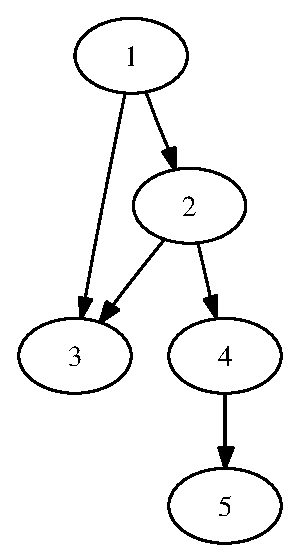
\epsfig{file=Figures/graph0,scale=0.6}

  \caption{A simple graph.}
  \label{fig:graph0}
\end{figure}



\noindent
The graph given by the relation \texttt{R} contains only the direct connections of vertices.  For example, in
the graph shown in Figure \ref{fig:graph0}, there is a direct connection from vertex $1$ to vertex $2$ and
another direct connection from vertex $2$ to vertex $4$.  Intuitively, vertex $4$ is reachable from vertex $1$,
since from vertex $1$ we can first reach vertex $2$ and from vertex $2$ we can then reach vertex $4$.  However,
there is is no direct connection between the vertices $1$ and $4$.  To make this more formal, define
a \colorbox{amethyst}{\blue{path}} 
of a graph $R$ as a list of vertices
\\[0.2cm]
\hspace*{1.3cm}
$[x_1, x_2, \cdots, x_n]$ \quad such that \quad $\pair(x_i,x_{i+1}) \in R$ \quad for all $i=1,\cdots,n-1$.
\\[0.2cm]
In this case, the path $[x_1, x_2, \cdots, x_n]$ is written as
\\[0.2cm]
\hspace*{1.3cm}
$x_1 \mapsto x_2 \mapsto \cdots \mapsto x_n$
\\[0.2cm]
and has the \blue{length} $n-1$.  It is important to note that the length of a path
$[x_1,x_2,\cdots,x_n]$ is defined as the number of edges connecting the vertices and not as the
number of vertices appearing in the path.

Furthermore,  two vertices $a$ and $b$ are said to be \colorbox{amethyst}{\blue{connected}} iff there exists a path
\\[0.2cm]
\hspace*{1.3cm}
$[x_1,\cdots,x_n]$ \quad such that \quad $a = x_1$ \quad and \quad $b = x_n$.
\\[0.2cm]
The goal of this section is to develop an algorithm that checks whether two vertices $a$ and $b$ are connected.
Furthermore, we want to be able to compute the corresponding path connecting the vertices $a$ and $b$.


\subsection{Computing the Transitive Closure of a Relation}
We have already noted that a graph can be represented as the set of its edges and hence as a \blue{relation}.
In order to decide whether there is a path connecting two vertices we have to compute the 
\href{https://en.wikipedia.org/wiki/Transitive_closure}{transitive closure} $R^+$ of a relation $R$.  
In the \href{https://github.com/karlstroetmann/Lineare-Algebra/blob/master/Script/lineare-algebra.pdf}{math lecture}
we have seen that the transitive closure $R^+$ can be computed as follows:
\\[0.2cm]
\hspace*{1.3cm}
$R^+ = \bigcup\limits_{n=1}^{\infty} R^n = R^1 \cup R^2 \cup R^3 \cup \cdots$  
\\[0.2cm]
Initially, this formula might look intimidating as it suggests an infinite computation.
Fortunately, it turns out that we do not have to compute all powers of the form $R^n$.  Let me
explain the reason that allows us to cut the computation short.  
\begin{enumerate}
\item $R$ is the set of direct connections between two vertices.
\item $R^2$ is the same as $R \circ R$ and this relational product is defined as
      \\[0.2cm]
      \hspace*{1.3cm}
       $R \circ R = \{ \pair(x,z) \mid \exists y \colon \pair(x,y) \in R \wedge \pair(y,z) \in R \}$.
      \\[0.2cm]
      Hence, $R \circ R$ contains those pairs $\pair(x,z)$ that are connected via one intermediate vertex $y$,
      i.e.~there is a path of the form $x \mapsto y \mapsto z$ that connects $x$ and $z$.  This path
      has length 2.  In general, we can show by induction that $R^n$ connect those pairs that are
      connected by a path of length $n$.  The induction step of this proof runs as follows:
\item $R^{n+1}$ is defined as $R \circ R^{n}$ and therefore we have
      \\[0.2cm]
      \hspace*{1.3cm}
      $R \circ R^n = \{ \pair(x,z) \mid \exists y \colon \pair(x,y) \in R \wedge \pair(y,z) \in R^n \}$.
      \\[0.2cm]
      As $\pair(y,z) \in R^n$, the induction hypothesis guarantees that the vertices $y$ and $z$ are
      connected by a path of length $n$.  Hence, this 
      path has the form
      \\[0.2cm]
      \hspace*{1.3cm}
      $\underbrace{y \mapsto \cdots \mapsto z}_{\mbox{\scriptsize path of length $n$.}}$
      \\[0.2cm]
      Adding $x$ at the front of this path will produce the path
      \\[0.2cm]
      \hspace*{1.3cm}
      $x \mapsto y \mapsto \cdots \mapsto z$.
      \\[0.2cm]
      This path has a length of $1 + n = n + 1$ and, furthermore, connects $x$ and $z$.  Hence $R^{n+1}$
      contains those pairs $\pair(x, z)$ that are connected by a path of length $n+1$.
\end{enumerate}
Now the important observation is the following. The set of all vertices is finite.  For the arguments sake, let
us assume there are $k$ vertices.  But then every path that has a length of  $k$ or greater must contain one
vertex that is visited at least twice and hence this path is longer than necessary, i.e.~there is a shorter path that
connects the same vertices.  Therefore, for a finite graph with $k$ vertices, the formula to compute the
transitive closure can be simplified as follows:
\\[0.2cm]
\hspace*{1.3cm} 
$\ds R^+ = \bigcup\limits_{i=1}^{k-1} R^i$.
\\[0.2cm]
While we could use this formula as its stands, it is more efficient to use a \blue{fixed-point iteration} instead.
To this end, we prove that the transitive closure $R^+$ satisfies the following equation:
\begin{equation}
  \label{fixpunkt}
  R^+ = R \cup R \circ R^+. 
\end{equation}
Let me remind you that the precedence of the operator $\circ$ 
is higher than the precedence of the operator $\cup$.  Therefore, the expression $R \cup R \circ R^+$ is parenthesized
as $R \cup (R \circ R^+)$.  Equation \ref{fixpunkt} can be proven algebraically.  We have:
\\[0.2cm]
\hspace*{1.3cm}
$
\begin{array}{cll}
    & R \cup R \circ R^+ \\[0.2cm]
  = & R \cup R \circ \bigcup\limits_{i=1}^{\infty} R^i \\[0.4cm]
  = & R \cup R \circ \bigl(R^1 \cup R^2 \cup R^3 \cup \cdots \bigr) \\[0.2cm]
  = & R \cup \bigl(R \circ R^1 \cup R \circ R^2 \cup R \circ R^3 \cup \cdots \bigr) \\[0.2cm]
  = & R \cup \bigl(R^2 \cup R^3 \cup  R^4 \cup \cdots \bigr)  \\[0.2cm]
  = & R^1 \cup \bigl(R^2 \cup R^3 \cup  R^4 \cup \cdots \bigr) \\[0.2cm]
  = & \bigcup\limits_{i=1}^{\infty} R^i \\[0.4cm]
  = & R^+.
\end{array}
$
\\[0.2cm]
Equation  \ref{fixpunkt} can now be used to compute $R^+$ via a fixed-point iteration.
To this end, let us define a sequence of relations $(T_n)_{n \in \mathbb{N}}$ by induction on $n$:
\begin{enumerate}
\item[I.A.] $n = 0$: 

            $T_0 = R$
\item[I.S.] $n \mapsto n+1$:

            $T_{n+1} = R \cup R \circ T_n$. 
\end{enumerate}
The relation  $T_n$ can be expressed via the relation $R$, we have
\begin{enumerate}
\item $T_0 = R$.
\item $T_1 = R \cup R \circ T_0 = R \cup R \circ R = R^1 \cup R^2$.
\item$\begin{array}[t]{lcl}
       T_2  & = & R \cup R \circ T_1 \\
            & = & R \cup R \circ (R^1 \cup R^2) \\
            & = & R^1 \cup R^2 \cup R^3. \\
       \end{array}
      $
\end{enumerate}
In general, we can show by induction that
\\[0.2cm]
\hspace*{1.3cm}
$T_n = \bigcup\limits_{i=1}^{n+1} R^i$
\\[0.2cm]
holds for all $n \in \mathbb{N}$.  The base case of this proof is immediate form the definition of $T_0$.
In the induction step we observe the following:
\\[0.2cm]
\hspace*{1.3cm}
$
 \begin{array}{lcll}
   T_{n+1} & = & \ds R \cup R \circ T_n & \mbox{(by definition)} \\[0.2cm]
           & = & \ds R \cup R \circ \biggl(\bigcup\limits_{i=1}^{n+1} R^i\biggr) &
                 \mbox{(by induction hypothesis)} \\[0.4cm]
           & = & \ds R \cup R \circ \left(R \cup \cdots \cup R^{n+1}\right) \\[0.2cm] 
           & = & \ds R \cup R^2 \cup \cdots \cup R^{n+2}  &
                 \mbox{(by the distributivity of $\circ$ over $\cup$)} \\[0.2cm]
           & = & \ds \bigcup\limits_{i=1}^{n+2} R^i & \Box 
   \end{array}
$
\\[0.2cm]
The sequence $(T_n)_{n\in\mathbb{N}}$ has another useful property:  It is 
\blue{monotonically increasing}.  In general, a sequence of sets $(X_n)_{n\in\mathbb{N}}$ is called
\blue{monotonically increasing} iff we have
\\[0.2cm]
\hspace*{1.3cm}
$\forall n \in \mathbb{N}: X_n \subseteq X_{n+1}$,
\\[0.2cm]
i.e.~the sets $X_n$ get bigger with growing index $n$.
The monotonicity of the sequence  $(T_n)_{n \in \mathbb{N}}$ is an immediate consequence of the equation
\\[0.2cm]
\hspace*{1.3cm}
$\ds T_n = \bigcup\limits_{i=1}^{n+1} R^i$ 
\\[0.2cm]
because we have:
\\[0.2cm]
\hspace*{1.3cm}
$
\begin{array}[t]{llcl}
                & \ds T_n \subseteq T_{n+1} \\[0.2cm]
\Leftrightarrow & \ds \bigcup\limits_{i=1}^{n+1} R^i \subseteq \bigcup\limits_{i=1}^{n+2} R^i \\[0.5cm]
\Leftrightarrow & \ds \bigcup\limits_{i=1}^{n+1} R^i \subseteq \bigcup\limits_{i=1}^{n+1} R^i \cup R^{n+2} \\
\end{array}
$
\\[0.2cm]
If the relation  $R$ is finite, then the transitive closure $R^+$ is finite, too.  The sets $T_n$ 
are all subsets of $R^+$ because we have
\\[0.2cm]
\hspace*{1.3cm}
$\ds T_n = \bigcup\limits_{i=1}^{n+1} R^i \subseteq \bigcup\limits_{i=1}^{\infty} R^i = R^+$ \quad for all $n \in \mathbb{N}$.
\\[0.2cm]
Hence the sets $T_n$ can not grow indefinitely.  Because of the monotonicity of the sequence 
$(T_n)_{n\in\mathbb{N}}$ it follows that there exists an index  $k \in \mathbb{N}$ such that the sets $T_n$ do
not grow any further once $n$ has reached $k$, i.e.~we have
\\[0.2cm]
\hspace*{1.3cm}
$\ds \forall n \in \mathbb{N}:( n \geq k \rightarrow T_n = T_k)$.
\\[0.2cm]
But this implies that
\\[0.2cm]
\hspace*{1.3cm}
$\ds T_n = \bigcup\limits_{i=1}^{n+1} R^i = \bigcup\limits_{i=1}^{\infty} R^i = R^+$ 
\quad holds for all $n \geq k$.
\\[0.2cm]
Therefore, the algorithm for computing  $R^+$ iterates the equation 
\\[0.2cm]
\hspace*{1.3cm}
$\ds T_{n+1} = R \cup R \circ T_n$
\\[0.2cm]
until the equation  $T_{n+1} = T_n$ is satisfied, since this implies that $T_n = R^+$.


\begin{figure}[!ht]
  \centering
\begin{Verbatim}[ frame         = lines, 
                  framesep      = 0.3cm, 
                  labelposition = bottomline,
                  numbers       = left,
                  numbersep     = -0.2cm,
                  xleftmargin   = 0.8cm,
                  xrightmargin  = 0.8cm,
                ]
    transClosure = procedure(R) {
        T = R;
        while (true) {
            oldT = T;
            T    = R + product(R, T);
            if (T == oldT) {
                return T;
            }
        }
    };
    product = procedure(R1, R2) {
        return { [x,z] : [x,y] in R1, [y,z] in R2 };
    };
    R = { [1,2], [2,3], [1,3], [2,4], [4,5] };
    print( "R = ", R );
    print( "Computing the transitive closure of R:" );
    T = transClosure(R);
    print( "R+ = ", T );
\end{Verbatim} 
\vspace*{-0.3cm}
\caption{Computing the transitive closure.}  
\label{fig:transitive-closure.py}
\end{figure} %\$

\noindent
The program 
\href{https://github.com/karlstroetmann/Logik/blob/master/Python/transitive-closure.py}{\texttt{transitive-closure.py}}
that is shown in Figure
\ref{fig:transitive-closure.py} on page \pageref{fig:transitive-closure.py} shows an implementation of this idea.
The program produces the following output:
\begin{verbatim}
    R = {[1, 2], [2, 3], [1, 3], [2, 4], [4, 5]}
    Computing the transitive closure of R:
    R+ = {[1, 2], [1, 3], [1, 4], [1, 5], [2, 3], [2, 4], [2, 5], [4, 5]}
\end{verbatim}
The transitive closure $R^+$ of a relation $R$ has a very intuitive interpretation:
$R^+$:  It contains all pairs $\pair(x,y)$ such that there is a path leading from 
$x$ to $y$.  
The function $\texttt{product}(R_1, R_2)$ computes the relational product $R_1\circ R_2$ 
according to the formula
\\[0.2cm]
\hspace*{1.3cm}
$R_1 \circ R_2 = \{ \langle x, z \rangle \mid \exists y: \pair(x,y) \in R_1 \wedge \pair(y,z) \in R_2 \}$.
\\[0.2cm]
The implementation of the procedure \texttt{product} shows the most general way to define a set in
\textsl{Python}.  In general, a set can be defined via an expression of the form
\\[0.2cm]
\hspace*{1.3cm}
$\{\; \textsl{expr} \;\texttt{:}\; [x^{(1)}_1, \cdots, x^{(1)}_{n(1)}] \;\texttt{in}\; s_1,
     \cdots, [x^{(k)}_1, \cdots, x^{(k)}_{n(k)}] \;\texttt{in}\; s_k \;\texttt{|}\;
     \textsl{cond} \;\}
$.
\\[0.2cm]
Here, for all $i=1, \cdots, k$ the variable $s_i$ denotes a set of lists of length $n(i)$.  When the
expression given above is evaluated, the variables $x^{(i)}_1, \cdots, x^{(i)}_{n(i)}$ are replaced
by the corresponding values in the lists from the sets  $s_i$.  For example, if we define
\begin{verbatim}
    s1 = { [ 1, 2, 3 ], [ 5, 6, 7 ] };
    s2 = { [ "a", "b" ], [ "c", "d" ] };
    m = { [ x1, x2, x3, y1, y2 ] : [ x1, x2, x3 ] in s1, [ y1, y2 ] in s2 };
\end{verbatim}
then the set  \texttt{m} has the following value:
\begin{verbatim}
    { [1, 2, 3, "a", "b"], [5, 6, 7, "c", "d"],  
      [1, 2, 3, "c", "d"], [5, 6, 7, "a", "b"] }
\end{verbatim}


\subsection{Computing the Paths}
So far, given a graph represented by a relation $R$ and two vertices $x$ and $y$, we can only check
whether there is a path leading from $x$ to $y$, but we cannot compute this path.  In this
subsection we will extend the procedure \texttt{transClosure} so that it will also compute the
corresponding path.  The main idea is to extend the notion of a relational product to the notion of
a \blue{path product}, where a \blue{path product} is defined on sets of paths.  In order to do so,
we introduce three functions for lists.
\begin{enumerate}
\item Given a list $p$, the function $\texttt{first}(p)$ returns the first element of $p$: 
      \\[0.2cm]
      \hspace*{1.3cm}
      $\texttt{first}\bigl([x_1,\cdots,x_m]\bigr) = x_1$.
\item Given a list $p$, the function $\texttt{last}(p)$ returns the last element of $p$: 
      \\[0.2cm]
      \hspace*{1.3cm}
      $\texttt{last}\bigl([x_1,\cdots,x_m]\bigl) = x_m$.
\item If $p = [ x_1, \cdots, x_m ]$ and $q =[ y_1, \cdots, y_n ]$ are two path such that
      $\texttt{first}(q) = \texttt{last}(p)$, we define the \blue{join} of $p$ and $q$ as \\[0.2cm]
      \hspace*{1.3cm}
      $p \oplus q = [x_1, \cdots, x_m, y_2, \cdots, y_n ]$.
\end{enumerate}
If $P_1$ and $P_2$ are sets of paths, we define the  \blue{path product} of
$P_1$ and $P_2$ as follows: \\[0.2cm]
\hspace*{1.3cm} 
$P_1 \bullet P_2 = 
\bigl\{\; p_1 \oplus p_2 \mid p_1 \in P_1 \wedge p_2 \in P_2 \wedge \texttt{last}(p_1) =
\texttt{first}(p_2) \;\bigr\}
$.

\begin{figure}[!ht]
  \centering
\begin{Verbatim}[ frame         = lines, 
                  framesep      = 0.3cm, 
                  labelposition = bottomline,
                  numbers       = left,
                  numbersep     = -0.2cm,
                  xleftmargin   = 0.8cm,
                  xrightmargin  = 0.8cm,
                ]
    transClosure = procedure(R) {
        P = R;
        while (true) {
            oldP = P;
            P    = R + pathProduct(R, P);
            print(P);
            if (P == oldP) {
                return P;
            }
        }
    };
    pathProduct = procedure(P, Q) {
        return { join(x, y) : x in P, y in Q | x[-1] == y[1] };
    };    
    join = procedure(p, q) {
        return p + q[2..];
    };
    R = { [1,2], [2,3], [1,3], [2,4], [4,5] };
    print( "R = ", R );
    print( "computing all paths" );
    P = transClosure(R);
    print( "P = ", P );
\end{Verbatim} 
\vspace*{-0.3cm}
\caption{Computing all connections.}  \label{fig:path.py}
\end{figure} %\$

\begin{figure}[!ht]
  \centering
  \vspace*{-9cm}

  \epsfig{file=Figures/graph-zykl,scale=0.5}
  \vspace*{-1cm}

  \caption{A graph with a cycle.}
  \label{fig:graph-zykl}
\end{figure}

Using the notion of a \blue{path product} we are able to extend the program shown in Figure
\ref{fig:transitive-closure.py} such that it computes all paths between two vertices.
The resulting program
\href{https://github.com/karlstroetmann/Logik/blob/master/Python/path.py}{\texttt{path.py}}
is shown in Figure \ref{fig:path.py} on page \pageref{fig:path.py}.
Unfortunately, the program does not work any more if the graph is \blue{cyclic}.  A graph is defined
to be \blue{cyclic} if there is a path of length greater than $1$ that starts and ends at the same
vertex.  This path is then called a \blue{cycle}.
Figure \ref{fig:graph-zykl} on page \pageref{fig:graph-zykl} shows a cyclic graph.  This graph is
cyclic because it contains the path
\\[0.2cm]
\hspace*{1.3cm}
\texttt{[1, 2, 4, 1]}
\\[0.2cm]
and this path is a cycle.
The problem with this graph is that it contains an infinite number of paths that connect the vertex
1 with the vertex 2: \\[0.2cm]
\hspace*{1.3cm}
$[ 1, 2 ]$, $[ 1, 2, 4, 1, 2 ]$, 
$[ 1, 2, 4, 1, 2, 4, 1, 2 ]$, 
$[ 1, 2, 4, 1, 2, 4, 1, 2, 4, 1, 4 ]$, $\cdots$
\\[0.2cm]
Of course, there is no point in computing a path that visits a vertex more than once as these paths
contain cycles.  Our goal is to eliminate all those paths that contain cycles.


\begin{figure}[!ht]
  \centering
\begin{Verbatim}[ numbers       = left,
                  numbersep     = -0.2cm,
                  frame         = lines, 
                  framesep      = 0.3cm, 
                  labelposition = bottomline,
                  xleftmargin   = 0.0cm,
                  xrightmargin  = 0.0cm,
                ]
    pathProduct = procedure(P, Q) {
        return { join(x,y) : x in P, y in Q | x[-1] == y[1] && noCycle(x, y) };
    };
    noCycle = procedure(L1, L2) {
        return #({ x : x in L1 } * { x : x in L2 }) == 1;
    };
\end{Verbatim} 
\vspace*{-0.3cm}
\caption{Computing the connections in a cyclic graph.}  
\label{fig:path-cyclic.py}
\end{figure} %\$

Figure \ref{fig:path-cyclic.py} on page shows how the implementation of the function
\texttt{pathProduct} has to be changed so that the resulting program
\href{https://github.com/karlstroetmann/Logik/blob/master/Python/path-cyclic.py}{\texttt{path-cyclic.py}}
works also for cyclic graphs. 
\begin{enumerate}
\item In line 2, we compute only those paths that are not cyclic.
\item Line 5 tests, whether the join  $\texttt{L1} \oplus \texttt{L2}$ is cyclic.  The join
      of \texttt{L1} and \texttt{L2} is cyclic iff the lists \texttt{L1} and \texttt{L2} have more
      than one common element. 
      The lists \texttt{L1} and \texttt{L2} will always have at least one common element, as we join
      these lists only if the last element of \texttt{L1} is equal to the first element of  \texttt{L2}.
      If there would be an another vertex common to \texttt{L1} and \texttt{L2}, then the path
      $\texttt{L1} \oplus \texttt{L2}$ would be cyclic.
\end{enumerate}

In general, we are not really interested to compute all possible paths between two given vertices
\texttt{x} and \texttt{y}.  Instead, we just want to compute the shortest path leading from \texttt{x} to \texttt{y}.
Figure \ref{fig:find-path.py} on page \pageref{fig:find-path.py} shows the procedure \texttt{reachable}. 
This procedure takes three arguments:
\begin{enumerate}
\item \texttt{x} and \texttt{y} are vertices of a graph.
\item \texttt{R} is a binary relation representing a directed graph.
\end{enumerate}
The call  \texttt{reachable(x, y, R)} checks whether \texttt{x} and \texttt{y} are connected and, furthermore,
computes the shortest path from \texttt{x} to \texttt{y}, provided such a path exists.
The complete program can be found in the file
\href{https://github.com/karlstroetmann/Logik/blob/master/Python/find-path.py}{\texttt{find-path.py}}.
Next, we discuss the implementation of the procedure  \texttt{reachable}.
\begin{enumerate}
\item Line 2 initializes the set \texttt{P}.  After $n$ iterations, this set will contain all paths
      that start in the vertex \texttt{x} and that have a length of at most $n$.

      Initially, there is just the trivial path \texttt{[x]} that starts in \texttt{x} and has
      length $0$.
\item Line 5 tries to extend all previously computed paths by one step.
      If we are lucky, the set \texttt{P} is increased in this step.
\item Line 6 selects all those paths from the set \texttt{P} that lead to the vertex \texttt{y}.
      These paths are stored in the set \texttt{Found}.
\item Line 7 checks whether we have indeed found a path ending at \texttt{y}.  This is the case if
      the set \texttt{Found} is not empty.  
      In this case, we return any of these paths.
\item If we have not yet found the vertex \texttt{y} and, furthermore, we have not been able to find
      any new paths during this iteration,  the procedure returns in line 11.
      As the \texttt{return} statement in line 11 does not return a value, the procedure will
      instead return the undefined value $\Omega$.
\end{enumerate}
The procedure call \texttt{reachable(x,y R)} will compute the \textbf{shortest} path connecting
\texttt{x} and \texttt{y} because it computes path with increasing length.  The first iteration
computes all paths starting in \texttt{x} that have a length of at most 1, the second iteration
computes all paths starting in \texttt{x} that have a length of at most 2, and in general the $n$-th
iteration computes all paths starting in \texttt{x} that have a length of at most $n$.  Hence, if
there is a path of length $n$, then this path will be found in the $n$-iteration unless a shorter path has
already been found in a previous iteration.  

\remarkEng
The algorithm described above is known as 
\href{https://en.wikipedia.org/wiki/Breadth-first_search}{breadth first search}. \eox 



\begin{figure}[!ht]
  \centering
\begin{Verbatim}[ frame         = lines, 
                  framesep      = 0.3cm, 
                  labelposition = bottomline,
                  numbers       = left,
                  numbersep     = -0.2cm,
                  xleftmargin   = 0.8cm,
                  xrightmargin  = 0.8cm,
                ]
    reachable = procedure(x, y, R) {
        P = { [x] };
        while (true) {
            oldP  = P;
            P     = P + pathProduct(P, R);
            Found = { l : l in P | l[-1] == y };
            if (Found != {}) {
                return arb(Found);
            }
            if (P == oldP) {
                return;
            }
        }
    };
\end{Verbatim} 
\vspace*{-0.3cm}
\caption{Finding the shortest path between two vertices.}  
\label{fig:find-path.py}
\end{figure}

\subsection{The Wolf, the Goat, and the Cabbage}
Next, we present an application of the theory developed so far.  We solve a problem from that has puzzled
the greatest agricultural economists for centuries.  The puzzle we want to solve is known as the 
\href{http://jeux.lulu.pagesperso-orange.fr/html/anglais/loupChe/loupChe1.htm}{wolf-goat-cabbage puzzle}:  
\vspace*{0.3cm}

\begin{minipage}[c]{14cm}
{\sl
An agricultural economist has to sell a wolf, a goat, and a cabbage on a market place.  In order to
reach the market place, she has to cross a river.  The boat that she can use is so small that it can
only accommodate either the goat, the wolf, or the cabbage in addition to the agricultural economist.
Now if the agricultural economist leaves the wolf alone with the goat, the wolf will eat the goat.
If, instead, the agricultural economist leaves the goat with the cabbage, the goat will eat the cabbage.
Is it possible for the agricultural economist to develop a schedule that allows her to cross the river
without either the goat or the cabbage being eaten?
}
\end{minipage}
\vspace*{0.3cm}

\noindent
In order to compute a schedule, we first have to model the problem.  The various \blue{states} of the problem will
be regarded as \blue{vertices} of a graph and this graph will be represented as a binary relation.
To this end we define the set
\\[0.2cm]
\hspace*{1.3cm} 
$\texttt{All} = \{ \squote{farmer}, \squote{wolf}, \squote{goat},\squote{cabbage} \}$.
\\[0.2cm]
Every node will be represented as a subset \texttt{S} of the set \texttt{All}.  The idea is that the set \texttt{S}
specifies those objects that are on the left side of the river.  We assume that initially the farmer
is on the left side of the river. 
Therefore, the set of all possible states can be defined as the set
\begin{verbatim}
        P = { S : S in 2 ** All | !problem(S) && !problem(All - S) };
\end{verbatim}
Here, we have used the procedure \texttt{problem} to check whether a given set \texttt{S} has a problem. 
Note that since \texttt{S} is the set of objects on the left side, the expression $\texttt{All - S}$
computes the set of objects on the right side of the river.

Next, a set \texttt{S} of objects has a problem if both of the following conditions
are satisfied:
\begin{enumerate}
\item The farmer is not an element of \texttt{S} and
\item either \texttt{S} contains both the goat and the cabbage or \texttt{S} contains both the wolf and the goat.
\end{enumerate}
Therefore, we can implement the function \texttt{problem} as follows:

\begin{verbatim}
    problem = procedure(S) {
        return !("farmer" in S)                                     && 
               ({"goat", "cabbage"} <= S || {"wolf", "goat"} <= S);
    };
\end{verbatim}
We proceed to compute the relation \texttt{R} that contains all possible transitions between
different states.  We will compute \texttt{R} using the formula:
\\[0.2cm]
\hspace*{0.75cm}
\texttt{R = R1 + R2;}
\\[0.2cm]
Here \texttt{R1} describes the transitions that result from the farmer crossing the river from left
to right, while \texttt{R2} describes the transitions that result from the farmer crossing the river
from right to left.  We can define the relation \texttt{R1} as follows:
\begin{verbatim}
    R1  = { [S, S - B]: S in P, B in 2 ** S
                       | S - B in P && "farmer" in B && #B <= 2
           };
\end{verbatim}
Let us explain this definition in detail:
\begin{enumerate}
\item Initially, \texttt{S} is the set of objects on the left side of the river.  Hence, \texttt{S}
      is an element of the set of all states that we have defined as \texttt{P}.
\item \texttt{B} is the set of objects that are put into the boat and that do cross the river.  Of
      course, for an object to go into the boat is has to be on the left side of the river to begin
      with.  Therefore, \texttt{B} is a subset of \texttt{S} and hence an element of the power set
      of \texttt{S}. 
\item Then  \texttt{S-B} is the set of objects that are left on the left side of the river after
      the boat has crossed.  Of course, the new state \texttt{S-B} has to be a state that does not
      have a problem.  Therefore, we check that \texttt{S-B} is an element of \texttt{P}.
\item Furthermore, the farmer has to be in the boat.  This explains the condition 
      \\[0.2cm]
      \hspace*{1.3cm}
      \texttt{\symbol{39}farmer\symbol{39} in B}.
\item Finally, the boat can only have two passengers.  Therefore, we have added the condition
      \\[0.2cm]
      \hspace*{1.3cm}
      \texttt{\#B <= 2}.
\end{enumerate}
Next, we have to define the relation \texttt{R2}.  However, as crossing the river from right to left
is just the reverse of crossing the river from left to right, \texttt{R2} is just the inverse of
\texttt{R1}.   Hence we define:
\\[0.2cm]
\hspace*{1.3cm}
\texttt{R2  = \{ [y, x] : [x, y] in R1 \};}
\\[0.2cm]
Finally, the start state has all objects on the left side.  Therefore, we have
\\[0.2cm]
\hspace*{1.3cm}
\texttt{start = All;}
\\[0.2cm]
In the end, all objects have to be on the right side of the river.  That means that nothing is left
on the left side.  Therefore, we define
\\[0.2cm]
\hspace*{1.3cm}
\texttt{goal = \{\};}
\\[0.2cm]
Figure \ref{fig:wolf-ziege} on page \pageref{fig:wolf-ziege} shows the program
\href{https://github.com/karlstroetmann/Logik/blob/master/Python/wolf-goat-cabbage.py}{\texttt{wolf-goat-cabbage.py}}
that combines the statements shown so far.  The solution computed by this program is shown in Figure
 \ref{fig:wolf-ziege-solution}.

\begin{figure}[!ht]
  \centering
\begin{Verbatim}[ codes         = {\catcode`$=3\catcode`_=8\catcode`^=7},
                  frame         = lines, 
                  framesep      = 0.3cm, 
                  labelposition = bottomline,
                  numbers       = left,
                  numbersep     = -0.2cm,
                  xleftmargin   = 0.8cm,
                  xrightmargin  = 0.8cm,
                ]
    problem = procedure(S) {
        return !("farmer" in S)                                     && 
               ({"goat", "cabbage"} <= S || {"wolf", "goat"} <= S);
    };
    
    All = { "farmer", "wolf", "goat", "cabbage" };
    P   = { S : S in 2 ** All | !problem(S) && !problem(All - S) };
    R1  = { [S, S - B]: S in P, B in 2 ** S
                       | S - B in P && "farmer" in B && #B <= 2
           };
    R2  = { [y, x] : [x, y] in R1 };
    R   = R1 + R2;
    
    start = All;
    goal  = {};
    
    path  = reachable(start, goal, R);
\end{Verbatim} 
\vspace*{-0.3cm}
\caption{Solving the wolf-goat-cabbage problem.}  
\label{fig:wolf-ziege}
\end{figure}


\begin{figure}[!ht]
  \centering
\begin{Verbatim}[ codes         = {\catcode`$=3\catcode`_=8\catcode`^=7},
                  frame         = lines, 
                  framesep      = 0.3cm, 
                  labelposition = bottomline,
                  numbers       = left,
                  numbersep     = -0.2cm,
                  xleftmargin   = 0.8cm,
                  xrightmargin  = 0.8cm,
                ]
    {"cabbage", "farmer", "goat", "wolf"}                                 {}
                             >>>> {"farmer", "goat"} >>>> 
    {"cabbage", "wolf"}                                   {"farmer", "goat"}
                             <<<< {"farmer"} <<<< 
    {"cabbage", "farmer", "wolf"}                                   {"goat"}
                             >>>> {"farmer", "wolf"} >>>> 
    {"cabbage"}                                   {"farmer", "goat", "wolf"}
                             <<<< {"farmer", "goat"} <<<< 
    {"cabbage", "farmer", "goat"}                                   {"wolf"}
                             >>>> {"cabbage", "farmer"} >>>> 
    {"goat"}                                   {"cabbage", "farmer", "wolf"}
                             <<<< {"farmer"} <<<< 
    {"farmer", "goat"}                                   {"cabbage", "wolf"}
                             >>>> {"farmer", "goat"} >>>> 
    {}                                 {"cabbage", "farmer", "goat", "wolf"}
\end{Verbatim} 
\vspace*{-0.3cm}
\caption{A schedule for the agricultural economist.}  
\label{fig:wolf-ziege-solution}
\end{figure}


\section{Terms and Matching}
So far we have seen the basic data structures of \setlx\ like numbers, string, sets, and lists.
There is one more data structure that is supported by \setlx.  This is the data structure of
\colorbox{amethyst}{\blue{terms}}.  
This data structure is especially useful when we develop programs that deal with mathematical formulas.
For example, in this section we will develop a program that reads a string like 
\\[0.2cm]
\hspace*{1.3cm}
``\texttt{x * exp(x)}'',
\\[0.2cm]
interprets this string as describing the real valued function 
\\[0.2cm]
\hspace*{1.3cm}
$x \mapsto x \cdot \exp(x)$, 
\\[0.2cm]
and then takes the derivative of this function with respect to the variable $x$.  This program is
easy to implement if real valued functions are represented as terms.  The reason is that \setlx\ provides 
\colorbox{amethyst}{\blue{matching}} for terms.  We will define this notion later.  Matching
is one of the main ingredients of the programming language \href{https://en.wikipedia.org/wiki/Prolog}{Prolog}.
This programming language was quite popular in artificial intelligence during the eighties and has
inspired the matching that is available in \textsl{Python}.


\subsection{Constructing and Manipulating Terms}
In order to build terms, we first need \colorbox{amethyst}{\blue{functors}}.  It is important not to confuse functors with
function symbols.  Therefore, functors have to be preceded by the character  
``\texttt{@}''.
For example, the following strings can be used as functors:
\\[0.2cm]
\hspace*{1.3cm}
\texttt{@f}, \quad \texttt{@FabcXYZ}, \quad \texttt{@sum}, \quad \texttt{@Hugo\_}.
\\[0.2cm]
However, in the expression ``\texttt{@f}'', the string ``\texttt{f}'' is the functor.  The
character ``\texttt{@}'' is only used as an escape character that tells us that ``\texttt{f}'' is
not a function symbol but rather a functor.  Next, we define \colorbox{amethyst}{\blue{terms}}.  If $F$ is a functor and 
$t_1$, $t_2$, $\cdots$, are any values, i.e.~they could be number, strings, lists, sets, or terms
themselves, then
\\[0.2cm]
\hspace*{1.3cm}
$\texttt{@}F(t_1, t_2, \cdots, t_n)$
\\[0.2cm]
is a term.  Syntactically, terms look very similar to function calls.  The only difference between a function call
and a term is the following: 
\begin{enumerate}
\item A function call starts with a function symbol. 
\item A term starts with a functor. 
\end{enumerate}


\examplesEng
\begin{enumerate}
\item \texttt{@Address(\symbol{39}Coblitzallee 1-9\symbol{39}, 68163, \symbol{39}Mannheim\symbol{39})}

      is a term that represents an address.
\item \texttt{@product(@variable(\symbol{39}x\symbol{39}), @exp(@variable(\symbol{39}x\symbol{39})))}

      is a term that represents the  function $x \mapsto x \cdot \exp(x)$.  
      \eox
\end{enumerate}
At this point you might ask how terms are evaluated.  The answer is that terms
\colorbox{amethyst}{are not evaluated!}  
Terms are used to represent data in a way that is both concise and readable.  Hence, terms are values like
numbers, sets or strings.  As terms are values, they don't need to be evaluated.

Let us demonstrate a very simple application of terms.  Imagine that \setlx\ wouldn't provide lists as a native data
type.  Then, we could implement lists via terms.  First, we would use a functor to represent the empty list.
Let us choose the functor \texttt{nil} for this purpose.  Hence, we have
\\[0.2cm]
\hspace*{1.3cm}
$\texttt{@nil()} \;\widehat{=}\; \texttt{[]}$,
\\[0.2cm]
where we read the symbol ``$\widehat{=}$'' as ``corresponds to''.
Note that the parentheses after the functor  \texttt{nil} are \colorbox{amethyst}{necessary!}  Next, in order to represent
a list with first element $x$ and a list $r$ of remaining elements we use the functor \texttt{cons}.
Then we have the correspondence
\\[0.2cm]
\hspace*{1.3cm}
$\texttt{@cons}(x, r) \;\widehat{=}\; \texttt{[}x\texttt{]} + r$. 
\\[0.2cm]
Concretely, the list \texttt{[1,2,3]} is represented as the term
\\[0.2cm]
\hspace*{1.3cm}
\texttt{@cons(1, @cons(2, @cons(3, @nil())))}.
\\[0.2cm]
The programming language \textsl{Prolog} represents lists internally in a similar form.

\setlx\ provides two functions that allow us to extract the components of a term.  Furthermore, there is a
function for constructing terms.  These functions are described next.
\begin{enumerate}
\item The function \texttt{fct} returns the functor of a given term.
      If  $t$ is a term of the form $\at F(s_1,\cdots,s_n)$, then the result returned by the expression
      \\[0.2cm]
      \hspace*{1.3cm}
      $\texttt{fct}(\at F(s_1,\cdots,s_n))$
      \\[0.2cm]
      is the functor $F$ of this term.  For example the expression
      \\[0.2cm]
      \hspace*{1.3cm}
      \texttt{fct(@cons(1, @cons(2, @cons(3, @nil()))))}
      \\[0.2cm]
      returns the string  \texttt{\symbol{39}cons\symbol{39}} as its result.
\item The function \texttt{args} returns the arguments of a term.
      If  $t$ is a term of the form $\at F(s_1,\cdots,s_n)$, then
      \\[0.2cm]
      \hspace*{1.3cm}
      $\mathtt{args}(\at F(s_1,\cdots,s_n))$
      \\[0.2cm]
      returns the list $[s_1, \cdots, s_n]$. For example, the expression
      \\[0.2cm]
      \hspace*{1.3cm}
      \texttt{args(\at cons(1, \at cons(2, \at cons(3, \at nil()))))}
      \\[0.2cm]
      is evaluated as
      \\[0.2cm]
      \hspace*{1.3cm}
      \texttt{[1, \at cons(2, \at cons(3, \at nil()))]}.
\item If $f$ is the name of a functor and  $l$ is a list, then the function \texttt{makeTerm} can be invoked as
      \\[0.2cm]
      \hspace*{1.3cm}
      $t \;\mathtt{=}\; \texttt{makeTerm}(f,l)$.
      \\[0.2cm]
      This expression generates a term $t$ such that $f$ is the functor and $l$ is the list of its
      arguments.  Therefore we have
      \\[0.2cm]
      \hspace*{1.3cm}
      $\mathtt{fct}(t) = f$  \quad und \quad $\mathtt{args}(t) = l$.
      \\[0.2cm]
      For example, the expression
      \\[0.2cm]
      \hspace*{1.3cm}
      \texttt{makeTerm(\symbol{39}cons\symbol{39}, [ 1, \at nil() ])}
      \\[0.2cm]
      returns the result
      \\[0.2cm]
      \hspace*{1.3cm}
      \texttt{\at cons(1, \at nil())}.
\end{enumerate}

\begin{figure}[!ht]
\centering
\begin{Verbatim}[ frame         = lines, 
                  framesep      = 0.3cm, 
                  firstnumber   = 1,
                  labelposition = bottomline,
                  numbers       = left,
                  numbersep     = -0.2cm,
                  xleftmargin   = 0.8cm,
                  xrightmargin  = 0.8cm,
                ]
    append = procedure(l, x) {
        if (fct(l) == "nil") {
            return @cons(x, @nil());  
        }
        [head, tail] = args(l);
        return @cons(head, append(tail, x));
    };
    l = @cons(1, @cons(2, @cons(3, @nil()))); // corresponds to [1,2,3]
    print(append(l, 4));
\end{Verbatim}
\vspace*{-0.3cm}
\caption{Appending an element at the end of a list.}
\label{fig:append.py}
\end{figure}

Figure \ref{fig:append.py} on page \pageref{fig:append.py} shows the
program \href{https://github.com/karlstroetmann/Logik/blob/master/Python/append.py}{\texttt{append.py}}.
This program implements the function \texttt{append}.  As its first arguments, this function takes a list \texttt{l}
that is represented as a term.  As its second argument,  it takes an object \texttt{x}.  The purpose of the expression
\\[0.2cm]
\hspace*{1.3cm}
$\texttt{append}(\texttt{l}, \texttt{x})$
\\[0.2cm]
is to append the object \texttt{x} at the end of the list \texttt{l}.  The implementation of the function \texttt{append}
assumes that the list \texttt{l} is represented as a term using the functors ``\texttt{cons}'' and ``\texttt{nil}''.
\begin{enumerate}
\item Line 2 checks whether the list  \texttt{l} is empty. The list \texttt{l} is empty iff we have
      $\texttt{l} = \texttt{\at nil()}$.  In the program we merely check the functor of the term \texttt{l}.  If the name of this functor is
      \texttt{\symbol{39}nil\symbol{39}}, then \texttt{l} is the empty list.
\item If \texttt{l} is not empty, then it must be a term of the form
      \\[0.2cm]
      \hspace*{1.3cm}
      $\texttt{l} = \texttt{\at cons(\textsl{head}, \textsl{tail})}$.
      \\[0.2cm]     
      Then, conceptually \texttt{head} is the first element of the list \texttt{l} and \texttt{tail} is the list of
      the remaining elements.  In this case, we need to recursively append \texttt{t} at the end of the list \texttt{tail}.
      Finally, the first element of the list \texttt{l}, which is called \texttt{head} in line 5, needs
      to be prepended to the list that is returned from the recursive invocation of \texttt{append}.
      This is done in line 6 by constructing the term 
      \\[0.2cm]
      \hspace*{1.3cm}
      \texttt{@cons(head, append(tail, x))}.
\end{enumerate}

\subsection{Matching}
It would be quite tedious if the functions \texttt{fct} and \texttt{args} were the only means to extract the
components of a term.  Figure \ref{fig:append-match.py} on page \pageref{fig:append-match.py}
shows the program
\href{https://github.com/karlstroetmann/Logik/blob/master/Python/append-match.py}{\texttt{append-match.py}}, 
that uses \blue{matching} to implement the function \texttt{append}.  
Line 3 checks, whether the list  \texttt{l} is empty, i.e.~whether \texttt{l} is identical to the term 
\texttt{@nil()}.  Line 4 is more interesting, as it combines two actions.
\begin{enumerate}
\item It checks, whether the list \texttt{l} is a term that starts with the functor \texttt{cons}.
\item If \texttt{l} does indeed starts with the functor \texttt{cons}, the arguments of this functor are
      extracted and assigned to the variables \texttt{head} and \texttt{tail}.
\end{enumerate}
Hence, if the \texttt{match} statement in line 4 is successful, the equation
\\[0.2cm]
\hspace*{1.3cm}
$\texttt{l} = \texttt{@cons(head, tail)}$
\\[0.2cm]
holds afterwards.


\begin{figure}[!ht]
\centering
\begin{Verbatim}[ frame         = lines, 
                  framesep      = 0.3cm, 
                  firstnumber   = 1,
                  labelposition = bottomline,
                  numbers       = left,
                  numbersep     = -0.2cm,
                  xleftmargin   = 0.8cm,
                  xrightmargin  = 0.8cm,
                ]
    append = procedure(l, x) {
        match (l) {
            case @nil():            return @cons(x, @nil());
            case @cons(head, tail): return @cons(head, append(tail, x));
        }
    };
\end{Verbatim}
\vspace*{-0.3cm}
\caption{Implementing \texttt{append} using a \texttt{match} statement.}
\label{fig:append-match.py}
\end{figure}
In general, a \texttt{match} statement has the structure that is shown in Figure \ref{fig:match}.
Here, $e$ is any expression that yields a term when evaluated.  The expressions 
$t_1$, $\cdots$, $t_n$ are so called \blue{patterns} that contain variables.  When the \texttt{match} statement
is executed, \textsl{Python} tries to bind the variables occurring in the pattern $t_1$ such that the resulting
expression is equal to $e$.  If this succeeds, the statements in  $\textsl{body}_1$ are executed and the
execution of the \texttt{match} statement ends.
Otherwise, the patterns $t_2$, $\cdots$, $t_n$ are tried one by one.  If the pattern $t_i$ is successfully
matched to $e$, the statements in $\textsl{body}_i$ are executed and the execution of the \texttt{match}
statement end.  If none of the patterns $t_1$, $\cdots$, $t_n$ can be matched with $e$, the statements in
$\textsl{body}_{n+1}$ are executed.


\begin{figure}[!ht]
  \centering
\begin{Verbatim}[ codes         = {\catcode`_=8\catcode`^=7},
                  frame         = lines, 
                  framesep      = 0.3cm, 
                  labelposition = bottomline,
                  numbers       = left,
                  numbersep     = -0.2cm,
                  commandchars  = \\\{\},
                  xleftmargin   = 0.8cm,
                  xrightmargin  = 0.8cm
                ]
      \texttt{\underline{match} (\(e\)) \{}
          \texttt{\underline{case}} \(t_1\) : \textsl{body}\(_1\) 
          \vdots
          \texttt{\underline{case}} \(t_n\) : \textsl{body}\(_n\)
          \texttt{\underline{default}:} \textsl{body}\(_{n+1}\)
      \texttt{\}}
\end{Verbatim}
\vspace*{-0.3cm}
\caption{Struktur eines \texttt{Match}-Blocks}  \label{fig:match}
\end{figure} 


\begin{figure}[!ht]
\centering
\begin{Verbatim}[ frame         = lines, 
                  framesep      = 0.3cm, 
                  firstnumber   = 1,
                  labelposition = bottomline,
                  numbers       = left,
                  numbersep     = -0.2cm,
                  xleftmargin   = 0.8cm,
                  xrightmargin  = 0.8cm,
                ]
    loadLibrary("termUtilities");  

    diff = procedure(t, x) {
        match (t) {
            case a + b :
                return diff(a, x) + diff(b, x);
            case a - b :
                return diff(a, x) - diff(b, x);
            case a * b :
                return diff(a, x) * b + a * diff(b, x);
            case a / b :
                return ( diff(a, x) * b - a * diff(b, x) ) / b * b;
            case a ** b :
                return diff( @exp(b * @ln(a)), x);
            case @ln(a) :
                return diff(a, x) / a;
            case @exp(a) :
                return diff(a, x) * @exp(a);
            case v | v == x :
                return 1;
            case y | isVariable(y) :  // must be different from x
                return 0;
            case n | isNumber(n):   
                return 0;  
         }
    };
    test = procedure(s) {
        t = parseTerm(s);
        v = parseTerm("x");
        d = diff(t, v);
        print("d/dx($s$) = $d$\n");
    };
    test("x ** x");
\end{Verbatim}
\vspace*{-0.3cm}
\caption{A function to perform symbolic differentiation.}
\label{fig:diff.py}
\end{figure}

\noindent
We close this section by showing an example that demonstrates the power of matching.
The function \texttt{diff} that is shown in Figure \ref{fig:diff.py} on page \pageref{fig:diff.py} is part
of the program
\href{https://github.com/karlstroetmann/Logik/blob/master/Python/diff.py}{\texttt{diff.py}}.
This function is called with two arguments.
\begin{enumerate}
\item The first argument \texttt{t} is a term that represents an arithmetical expression.
\item The second argument \texttt{x} is a term that represents a variable.
\end{enumerate}
The function \texttt{diff} interprets its argument \texttt{t} as a function of the variable
\texttt{x}.  We take the \href{https://en.wikipedia.org/wiki/Derivative}{derivative} of this
function with respect to the variable \texttt{x}.  For example, in order to compute the derivative of
the function
\\[0.2cm]
\hspace*{1.3cm}
$x \mapsto x^x$,
\\[0.2cm]
we can call the function  \texttt{diff} as follows:
\\[0.2cm]
\hspace*{1.3cm}
\texttt{diff(parseTerm(\symbol{39}x ** x\symbol{39}), parseTerm(\symbol{39}x\symbol{39}));}
\\[0.2cm]
Here, the function \texttt{parseTerm} is a function that is defined in the library \texttt{termUtilities}.
This function takes a string as input and converts this string into a term.  In order to use the function
\texttt{parseTerm}, we have to load the library that defines it.  This happens in line 1 of Figure
\ref{fig:diff.py}. 

Let us now discuss the implementation of the function \texttt{diff} in more detail.  
\begin{enumerate}
\item Line 5 makes use of the fact that the operator ``\texttt{+}'' can be applied to terms.
      The result is a term that has the functor ``\texttt{@@@sum}''.  However, this functor is hidden from the
      user and becomes only visible when we use the function \texttt{fct} to expose it.  For example, we can
      define a term \texttt{t} as follows:
      \\[0.2cm]
      \hspace*{1.3cm}
      \texttt{t = @f(1) + @g(2);}
      \\[0.2cm]
      Then \texttt{t} is a term that is displayed as ``\texttt{@f(1) + @g(2)}'', but the expression
      \texttt{fct(t)} returns the string
      \\[0.2cm]
      \hspace*{1.3cm}
      \texttt{"@@@sum"}.
      \\[0.2cm]
      There is no need to remember that the internal representation of the operator ``\texttt{+}'' as a functor
      is given as the string ``\texttt{@@@sum}'''.  The only thing that you have to keep in mind is
      the fact, that the operator ``\texttt{+}'' can be applied to terms.  The same is true for the
      other arithmetical operators ``\texttt{+}'', ``\texttt{-}'', ``\texttt{*}'', ``\texttt{/}'',
      ``\texttt{\symbol{37}}'', and ``\texttt{**}''.  Similarly, the logical operators
      ``\texttt{\&\&}'', ``\texttt{||}'', ``\texttt{!}'', ``\texttt{=>}'', and ``\texttt{<==>}'' can
      be used as functors.  Note, however, that the relational operators ``\texttt{<}'',
      ``\texttt{>}'', ``\texttt{<=}'', ``\texttt{>=}'' \colorbox{amethyst}{can not be used} to
      combine terms.  Finally, the operators ``\texttt{==}'' and ``\texttt{!=}'' can be used to
      check whether two terms are identical or different, respectively.  Hence, while these
      operators can be applied to terms, they return a Boolean value, not a term!
      
      As the operator ``\texttt{+}'' can be used as a functor, it can also be used in a pattern.  The
      pattern 
      \\[0.2cm]
      \hspace*{1.3cm}
      \texttt{a + b}
      \\[0.2cm]
      matches any term that can be written as a sum.  The derivative of a sum is computed by summing the
      derivatives of the components of the sum, i.e.~we have
      \\[0.2cm]
      \hspace*{1.3cm}
      $\ds \diff\bigl(f(x) + g(x)\bigr) = \diff f(x) + \diff g(x)$.
      \\[0.2cm]
      Therefore, the case where the term \texttt{t} has the form \texttt{a + b} can be dealt with by
      recursively computing the derivatives of \texttt{a} and \texttt{b} and adding them.  This
      happens in line 6.
\item Line 7 deals with the case where \texttt{t} is a difference.  Mathematically, the rule to take the
      derivative of a difference is
      \\[0.2cm]
      \hspace*{1.3cm}
      $\ds \diff\bigl(f(x) - g(x)\bigr) = \diff f(x) - \diff g(x)$.
      \\[0.2cm]
      This rule is implemented in line 8.
\item Line 9 deals with the case where \texttt{t} is a product.  The 
      \href{https://en.wikipedia.org/wiki/Product_rule}{product rule} is
      \\[0.2cm]
      \hspace*{1.3cm}
      $\ds \diff\bigl(f(x) \cdot g(x)\bigr) = \left(\diff f(x)\right)\cdot g(x) + f(x) \cdot \left(\diff g(x)\right)$.
      \\[0.2cm]
      This rule is implemented in line 10.
\item Line 11 deals with the case where \texttt{t} is a quotient.  The
      \href{https://en.wikipedia.org/wiki/Quotient_rule}{quotient rule} is 
      \\[0.2cm]
      \hspace*{1.3cm}
      $\ds \diff\left(\frac{f(x)}{g(x)}\right) = \frac{\left(\diff f(x)\right)\cdot g(x) - f(x)
        \cdot \left(\diff g(x)\right)}{g(x) \cdot g(x)}$.
      \\[0.2cm]
      This rule is implemented in line 12.
\item Line 13 deals with the case where \texttt{t} is a power.  Now in order to take the derivative of an
      expression of the form
      \\[0.2cm]
      \hspace*{1.3cm}
      $\ds f(x)^{g(x)}$
      \\[0.2cm]
      we first need to rewrite it using the following trick:
      \\[0.2cm]
      \hspace*{1.3cm}
      $\ds f(x)^{g(x)} = \exp\bigl(\ln\bigl(f(x)^{g(x)}\bigr)\bigr) = \exp\bigl(g(x) \cdot \ln(f(x))\bigr)$,
      \\[0.2cm]
      Then, we can recursively call \texttt{diff} for this expression.  This works, because the function
      \texttt{diff} can deal with both the exponential function $x \mapsto \exp(x)$ and with the natural
      logarithm $x \mapsto \ln(x)$.  This rewriting is done in line 14.
\item Line 15 deals with the case where \texttt{t} has the form $\ln\bigl(f(x)\bigr)$.  
      In order to take the derivative of this expression, we first need to know the derivative of the natural
      logarithm.  This derivative is given as 
      \\[0.2cm]
      \hspace*{1.3cm}
      $\ds \diff \ln(x) = \frac{1}{x}$.
      \\[0.2cm]
      Then, using the \href{https://en.wikipedia.org/wiki/Chain_rule}{chain rule} we have that
      \\[0.2cm]
      \hspace*{1.3cm}
      $\ds \diff \ln\bigl(f(x)\bigr) = \frac{\diff f(x)}{f(x)}$.
      \\[0.2cm]
      This rule is used in line 16.
\item Line 17 deals with the case where \texttt{t} has the form $\exp\bigl(f(x)\bigr)$.  
      In order to take the derivative of this expression, we first need to know the derivative of the 
      \href{https://en.wikipedia.org/wiki/Exponential_function}{exponential function}.  This derivative is given as 
      \\[0.2cm]
      \hspace*{1.3cm}
      $\ds \diff \exp(x) = \exp(x)$.
      \\[0.2cm]
      Then, using the \href{https://en.wikipedia.org/wiki/Chain_rule}{chain rule} we have that
      \\[0.2cm]
      \hspace*{1.3cm}
      $\ds \diff \exp\bigl(f(x)\bigr) = \left(\diff f(x)\right) \cdot \exp\bigl(f(x)\bigr)$.
      \\[0.2cm]
      This rule is used in line 18.
\item Line 19 deals with the case where \texttt{t} is a variable and happens to be the same variable as
      \texttt{x}.  This is checked using the condition
      \\[0.2cm]
      \hspace*{1.3cm}
      \texttt{v == x}
      \\[0.2cm]
      that is attached using the \blue{condition operator} ``\texttt{|}''.   Since we have
      \\[0.2cm]
      \hspace*{1.3cm}
      $\ds \frac{\mathrm{d}x}{\mathrm{d}x} = 1$,
      \\[0.2cm]
      the function \texttt{diff} returns \texttt{1} in this case.
\item Line 21 deals with the case where \texttt{t} is a variable.  As line 19 has already covered the case that
      \texttt{t} and \texttt{x} are the same variable, in this case the variable \texttt{x} must be different
      from \texttt{t}.  Therefore, with respect to \texttt{x} the term \texttt{t} can be seen as a constant and
      the derivative is \texttt{0}.
\item Line 23 covers the case where \texttt{t} is a number.  Note how we call \texttt{isNumber}
      after the condition operator ``\texttt{|}''.  As a number is a constant, the derivative is \texttt{0}.
\item Line 27 defines the procedure \texttt{test}.  This procedure takes a string \texttt{s} and transforms it
      into the term \texttt{t} via the function \texttt{parseTerm} defined in the library
      \texttt{termUtilities}.  Similarly, the string \texttt{"x"} is transformed into the term \texttt{v} that
      represents this variable.\footnote{Internally, this variable is represented as the term
      ``\texttt{@@@variable("x")}''.}
      Line 30 call the function \texttt{diff} using the term \texttt{t} and the variable \texttt{v}
      as arguments.  The resulting term is printed in line 31.
\item Line 33 shows how the function \texttt{test} can be called to compute the derivative $\diff x^x$.
\end{enumerate}


\section{Outlook}
This introductory chapter covers only a small part of the programming language  \textsl{Python}.  There are some
additional features of \setlx\ that will be discussed in the following chapters as we need them.
Furthermore,  \textsl{Python} is discussed in depth in the tutorial that can be found at the following address:
\\[0.2cm]
\hspace*{1.3cm}
\href{http://download.randoom.org/setlX/tutorial.pdf}{\texttt{http://download.randoom.org/setlX/tutorial.pdf}}


\remarkEng
Most of the algorithm that were presented in this chapter are not very efficient.  The main purpose of these
algorithms is to serve as examples that were presented for two reasons:
\begin{enumerate}
\item My first intention was to make the abstract notions introduced in set theory more accessible.  For
      example, the program to compute the transitive closure serves to illustrate both the notion of the
      relational product and the transitive closure.  Furthermore, it shows how these notions are useful in
      solving real world problems.
\item Second, these programs serve to introduce the programming language \setlx.
\end{enumerate}
Later, the lecture on
\href{https://github.com/karlstroetmann/Algorithms/blob/master/Lecture-Notes/algorithms.pdf}{algorithms}
will show how to develop efficient algorithms that are more efficient.
\vspace*{0.3cm}


\section{Reflection}
After having completed this chapter, you should be able to answer the following questions.
\begin{enumerate}
\item Which data types are supported in \textsl{Python}?
\item What are the different methods to define a set in \textsl{Python}?
\item Do you understand how to construct lists via iterator? 
\item How can lists be defined in \textsl{Python}?
\item How does \textsl{Python} support binary relations?
\item How does list slicing and list indexing work?
\item How does \textsl{Python} support terms?
\item How does a fixed-point algorithm work?
\item What type of control structures are supported in \textsl{Python}?
\item How can terms be defined and how does matching for terms work?
\end{enumerate}

%%% Local Variables: 
%%% mode: latex
%%% TeX-master: "logic"
%%% End: 


%\chapter{Applications and Case Studies}
This chapter contains a number of case studies designed to deepen our understanding of \textsl{Python}.

\section{Solving Equations via Fixed-Point Algorithms}
\blue{Fixed-Point iterations} are very important, both in computer science and in mathematics.  As a first
example, we show how to solve an equation via a fixed point iteration.  Suppose we want to solve the equation  
\\[0.2cm]
\hspace*{1.3cm} $x = \cos(x)$. \\[0.2cm]
Here, $x$ is a real number that we seek to compute.  Figure \ref{fig:xEqualsCosX.pdf} on page
\pageref{fig:xEqualsCosX.pdf} shows the graphs of the two functions  
\\[0.2cm]
\hspace*{1.3cm}
$y = x$  \quad and \quad $y = \cos(x)$.
\\[0.2cm]
Since the graphs of these functions intersect, it is obvious that there exists a value $x$ such that $x = \cos(x)$. 
Furthermore, from Figure \ref{fig:xEqualsCosX.pdf} it is obvious that this value of $x$ is bigger than $0.6$
and less than $0.8$. 

\begin{figure}[!ht]
  \hspace*{-3.0cm}
  \epsfig{file=Figures/xEqualsCosX.pdf,scale=0.6}

  \caption{The functions $y = x$ and $y = cos(x)$.}
  \label{fig:xEqualsCosX.pdf}
\end{figure}



A simple approach that lets us compute the exact value of $x$ is to use a
\href{https://en.wikipedia.org/wiki/Fixed-point_iteration}{fixed-point iteration}.  To this end, we
define the sequence $\bigl(x_n\bigr)_{n\in\mathbb{N}}$ inductively as follows:
\\[0.2cm]
\hspace*{1.3cm} 
$x_0 = 0$ \quad and \quad $x_{n+1} = \mathtt{cos}(x_n)$ \quad for all $n \in \mathbb{N}$. 
\\[0.2cm]
With the help of the 
\href{https://en.wikipedia.org/wiki/Banach_fixed-point_theorem}{Banach fixed-point theorem}\footnote{
  The Banach fixed-point theorem is discussed in the lecture on
  \href{https://en.wikipedia.org/wiki/Differential_calculus}{differential calculus}.  This lecture is part of the
  second semester.
}
it can be shown that this sequence converges to a solution of the equation $x = \cos(x)$, i.e.~if we define
\\[0.2cm]
\hspace*{1.3cm}
$\bar{x} = \lim\limits_{n\rightarrow\infty} x_n$,
\\[0.2cm]
then we have
\\[0.2cm]
\hspace*{1.3cm}
$\cos\bigl(\bar{x}\bigr) = \bar{x}$.
\\[0.2cm]
Figure \ref{fig:solve.py} on page \pageref{fig:solve.py} shows the program
\href{https://github.com/karlstroetmann/Logic/blob/master/Python/solve.py}{\texttt{solve.py}}
that uses this approach to solve the equation $x = \cos(x)$.


\begin{figure}[!ht]
  \centering
\begin{Verbatim}[ frame         = lines, 
                  framesep      = 0.3cm, 
                  labelposition = bottomline,
                  numbers       = left,
                  numbersep     = -0.2cm,
                  xleftmargin   = 0.8cm,
                  xrightmargin  = 0.8cm,
                ]
    import math
    
    x     = 1.0
    old_x = 0.0
    i     = 1
    while abs(x - old_x) >= 4.0E-16:
        old_x = x
        x = math.cos(x)
        print(f'{i} : {x}')
        i += 1
\end{Verbatim} 
\vspace*{-0.3cm}
\caption{Solving the equation $x = \cos(x)$ via fixed-point iteration.}  \label{fig:solve.py}
\end{figure} %\$

In this program, the iteration stops as soon as the difference between the variables \texttt{x} and 
\texttt{old\_x} is less that $4 \cdot 10^{-16}$.  Here, \texttt{x} corresponds to $x_{n+1}$, while \texttt{old\_x}
corresponds to $x_n$.  Once the values of $x_{n+1}$ and $x_n$ are sufficiently close, the execution of the \texttt{while} loop
terminates.
\href{https://github.com/karlstroetmann/Logic/blob/master/Python/Fixed-Point-Iteration.ipynb}{Fixed-Point-Iteration.ipynb}
shows a \textsl{Jupyter} notebook that implements fixed point iteration.


\begin{figure}[!ht]
\centering
\begin{Verbatim}[ frame         = lines, 
                  framesep      = 0.3cm, 
                  firstnumber   = 1,
                  labelposition = bottomline,
                  numbers       = left,
                  numbersep     = -0.2cm,
                  xleftmargin   = 0.8cm,
                  xrightmargin  = 0.8cm,
                ]
    from math import cos
    
    def solve(f, x0):
        """
        Solve the equation f(x) = x using a fixed point iteration.
        x0 is the start value.
        """
        x = x0
        for n in range(10000):  # at most 10000 iterations
            oldX = x;
            x    = f(x);
            if abs(x - oldX) < 1.0e-15: 
                return x;
    
    print("solution to x = cos(x): ", solve(cos, 0));
    print("solution to x = 1/(1+x):", solve(lambda x: 1/(1+x), 0));
\end{Verbatim}
\vspace*{-0.3cm}
\caption{A generic implementation of the fixed-point algorithm.}
\label{fig:fixpoint.py}
\end{figure}

Figure \ref{fig:fixpoint.py} on page \pageref{fig:fixpoint.py} shows the program
\href{https://github.com/karlstroetmann/Logic/blob/master/Python/fixpoint.py}{\texttt{fixpoint.py}}.
In this program we have implemented a function \texttt{solve} that takes two arguments.
\begin{enumerate}
\item \texttt{f} is a unary function.  The purpose of the \texttt{solve} is to compute the solution of the equation
      \\[0.2cm]
      \hspace*{1.3cm}
      $f(x) = x$.
      \\[0.2cm]
      This equation is solved with the help of a fixed-point algorithm.
\item \texttt{x0} is used as the initial value for the fixed-point iteration.
\end{enumerate}
Line 11 calls \texttt{solve} to compute the solution of the equation $x = \cos(x)$.
Line 12 solves the equation 
\\[0.2cm]
\hspace*{1.3cm}
$\ds x = \bruch{1}{1+x}$. 
\\[0.2cm]
This equation is equivalent to the quadratic equation $x^2 + x = 1$.  Note that we have defined the function
 $\ds x \mapsto \frac{1}{1+x}$ via the expression
 \\[0.2cm]
\hspace*{1.3cm}
\texttt{lambda x: 1/(1+x)}.
\\[0.2cm]
This expression is called an \blue{anonymous function} since we haven't given a name to the function.  

\remarkEng
The function \texttt{solve} is only able to solve the equation $f(x) = x$ if the function $f$ is a 
\href{https://en.wikipedia.org/wiki/Contraction_mapping}{contraction mapping}.  A function 
$f:\mathbb{R} \rightarrow \mathbb{R}$
is called a \blue{contraction mapping} iff 
\\[0.2cm]
\hspace*{1.3cm}
$|f(x) - f(y)| < |x - y|$ \quad for all $x,y \in \mathbb{R}$.
\\[0.2cm]
This notion will be discussed in more detail in the lecture on 
\href{https://github.com/karlstroetmann/Analysis/blob/master/Skript/analysis.pdf}{analysis} in the second
semester. \eox  

\section{Case Study: Computation of Poker Probabilities}
In this short section we are going to show how to compute probabilities for the
\href{https://en.wikipedia.org/wiki/Texas_hold_%27em}{\textsl{Texas Hold'em}} variation of 
\href{https://en.wikipedia.org/wiki/Poker}{poker}.   Texas Hold'em poker is played with a deck of 52
cards.  Every card has a \blue{value}.  This value is an element of the set
\\[0.2cm]
\hspace*{1.3cm} 
$\textsl{Values} = \{ 2, 3, 4, 5, 6, 7, 8, 9, 10, \textsl{Jack}, \textsl{Queen}, \textsl{King}, \textsl{Ace} \}$.
\\[0.2cm]
Furthermore, every card has a \blue{suit}.  This suit is an element of the set
\\[0.2cm]
\hspace*{1.3cm} 
$\textsl{Suits} = \{ \club, \mbox{$\color{red}{\heart}$}, \mbox{$\color{red}{\diamondsuit}$}, \spade \}$.
\\[0.2cm]
These suits are pronounced \blue{club}, \blue{heart}, \blue{diamond}, and \blue{spade}.
As a card is determined by its value and its suit, a card can be represented as a pair $\pair(v,s)$, where $v$
denotes the value while $s$ is the suit of the card.  Hence, the set of all cards can be represented as the set
\\[0.2cm]
\hspace*{1.3cm} 
$\textsl{Deck} = \bigl\{ \pair(v,s) \mid v \in \textsl{Values} \wedge \textsl{s} \in \textsl{Suits} \bigr\}$.
\\[0.2cm]
At the start of a game of Texas Hold'em, every player receives two cards.  These two cards are known
as the \blue{preflop} or the \blue{hole}.  Next, there is a \blue{bidding phase} where players can bet on their
cards.   After this bidding phase, the dealer puts three cards open on the table.  These three cards are
known as \blue{flop}.  Let us assume that a player has been dealt the set of cards
\\[0.2cm]
\hspace*{1.3cm}
$\{ \pair(3, \club), \pair(3, \spade) \}$.
\\[0.2cm]
This set of cards is known as a \blue{pocket pair}.  Then the player would like to know the probability
that the flop will contain another card with value $3$, as this would greatly increase her chance of
winning the game.  In order to compute this probability we have to compute the number of possible
flops that contain a card with the value $3$ and we have to divide this number by the number of all
possible flops:
\\[0.2cm]
\hspace*{1.3cm}
$\ds \frac{\;\mbox{number of flops containing a card with value $3$}\;}{\mbox{number of all possible flops}}$
\\[0.2cm]
The program
\href{https://github.com/karlstroetmann/Logic/blob/master/Python/poker-triple.py}{poker-triple.py}
shown in Figure \ref{fig:poker-triple.py} performs this computation.  We proceed to discuss this
program line by line.


\begin{figure}[!ht]
\centering
\begin{Verbatim}[ frame         = lines, 
                  framesep      = 0.3cm, 
                  labelposition = bottomline,
                  numbers       = left,
                  numbersep     = -0.2cm,
                  xleftmargin   = 0.0cm,
                  xrightmargin  = 0.0cm,
                ]
    Values = { "2", "3", "4", "5", "6", "7", "8", "9", "T", "J", "Q", "K", "A" } 
    Suits  = { "c", "h", "d", "s" }
    Deck   = { (v, s) for v in Values for s in Suits }
    Hole   = { ("3", "c"), ("3", "s") }
    Rest   = Deck - Hole
    Flops  = { (k1, k2, k3) for k1 in Rest for k2 in Rest for k3 in Rest 
                            if  len({ k1, k2, k3 }) == 3 
             }
    Trips  = { f for f in Flops if ("3", "d") in f or ("3", "h") in f }
    print(len(Trips) / len(Flops))
\end{Verbatim}
\vspace*{-0.3cm}
\caption{Computing a probability in poker.}
\label{fig:poker-triple.py}
\end{figure}

\begin{enumerate}
\item In line 1 the set \texttt{Values} is defined to be the set of all possible values that a card
      can take.  In defining this set we have made use of the following abbreviations:
      \begin{enumerate}
      \item ``\texttt{T}'' is short for ``\blue{Ten}'',
      \item ``\texttt{J}'' is short for ``\blue{Jack}'',
      \item ``\texttt{Q}'' is short for ``\blue{Queen}'',
      \item ``\texttt{K}'' is short for ``\blue{King}'', and
      \item ``\texttt{A}'' is short for ``\blue{Ace}''.
      \end{enumerate}
\item In line 2 the set \texttt{Suits} represents the possible suits of a card.  Here, we have used
      the following abbreviations:
      \begin{enumerate}
      \item ``\texttt{c}'' is short for $\club$ (\underline{c}lub), 
      \item ``\texttt{h}'' is short for \mbox{\color{red}{$\heart$}} (\underline{h}earts), 
      \item ``\texttt{d}'' is short for \mbox{\color{red}{$\diamondsuit$}} (\underline{d}iamonds), and 
      \item ``\texttt{s}'' is short for $\spade$ (\underline{s}pades). 
      \end{enumerate} 
\item Line 3 defines the set of all cards.  This set is stored as the variable \texttt{Deck}.  Every
      card is represented as a pair of the form $(v,s)$. Here, $v$ is the value of the card, while $s$ is its suit.
\item Line 4 defines the set \texttt{Hole}.  This set represents the two cards that have been given to our player.
\item The remaining cards are defined as the variable  \texttt{Rest} in line 5.
\item Line 6 computes the set of all possible flops.  Since the order of the cards in the flop does
      not matter, we use sets to represent these flops.  However, we have to take care that the flop
      does contain three \colorbox{amethyst}{different} cards.  Hence, we have to ensure that the three
      cards \texttt{k1}, \texttt{k2}, and \texttt{k3} that make up the flop satisfy the inequalities 
      \\[0.2cm]
      \hspace*{1.3cm}
      $\mathtt{k1} \not= \mathtt{k2}$, \quad $\mathtt{k1} \not= \mathtt{k3}$,  \quad and \quad $\mathtt{k2} \not= \mathtt{k3}$.
      \\[0.2cm]
      These inequalities are satisfied if and only if the set 
      $\{ \mathtt{k1}, \mathtt{k2}, \mathtt{k3} \}$ contains exactly three elements.  Hence, when
      choosing \texttt{k1}, \texttt{k2}, and \texttt{k3} we have to make sure that the condition
      \\[0.2cm]
      \hspace*{1.3cm}
      $\texttt{len}\bigl({\{ \mathtt{k1}, \mathtt{k2}, \mathtt{k3} \} \;\mathtt{==}\; 3 }\bigr)$
      \\[0.2cm]
      holds.
\item Line 9 computes the subset \texttt{Trips} of those flops that contain at least one card with a value of 3.
      As the 3 of clubs and the 3 of spades have already been dealt to our player, the only cards
      with value 3 that are left in the deck are the 3 of diamonds and the 3 of hearts.  Therefore, we are looking for
      those flops that contain one of these two cards.
\item Finally, the probability for obtaining another card with a value of 3 in the flop is computed as
      the ratio of the number of flops containing a card with a value of 3 to the number of all possible flops.
\end{enumerate}
When we run the program we see that the probability of improving a \blue{pocket pair} on the flop to \blue{trips} or better
is about  $11.8\%$.  A \textsl{Jupyter} notebook showcasing this computation outlined above can be fount at
\href{https://github.com/karlstroetmann/Logic/blob/master/Python/Poker.ipynb}{Poker.ipynb}.

\remarkEng
The method to compute probabilities that has been sketched above only works if the sets that have to
be computed are small enough to be retained in memory.  If this condition is
not satisfied we can use the \href{https://en.wikipedia.org/wiki/Monte_Carlo_method}{\emph{Monte Carlo method}} 
to compute the probabilities instead.  This method will be discussed in the lecture on 
\href{https://github.com/karlstroetmann/Algorithms/blob/master/Lecture-Notes/algorithms.pdf}{algorithms}.


\section{Finding a Path in a Graph}
In the following section, I will present an application that is more interesting since it is practically
relevant.  In order to prepare for this, we will now discuss the problem of finding a \blue{path} in a
\href{https://en.wikipedia.org/wiki/Directed_graph}{directed graph}. 
Abstractly, a \emph{directed graph} consists of \blue{vertices} and \blue{edges} that connect these vertices.  In an application, the
vertices could be towns and villages, while the edges would be interpreted as one-way streets connecting these
villages.  To simplify matters, let us assume for now that the vertices are given as natural numbers.  As the
edges represent connections between vertices,  the edges are represented as pairs of natural numbers.  Then,
the graph can be represented as the set of its edges, as the set of vertices is implicitly given once the edges
are known.  To make things concrete, let us consider an example.  In this case, the set of edges is called
\texttt{R} and is defined as follows:  
\\[0.2cm]
\hspace*{1.3cm}
$\texttt{R}\; \mathtt{=}\; \bigl\{ \pair(1,2), \pair(2,3), \pair(1,3), \pair(2,4), \pair(4,5) \bigr\}$.
\\[0.2cm]
In this graph, the set of vertices is given as
\\[0.2cm]
\hspace*{1.3cm}
$\{ 1, 2, 3, 4, 5 \}$.
\\[0.2cm]
This graph is shown in Figure \ref{fig:graph0} on page \pageref{fig:graph0}.  You should note that the
connections between vertices that are given in this graph are \blue{unidirectional}:  While there is a connection from
vertex $1$ to vertex $2$, there is no connection from vertex $2$ to vertex $1$.

 
\begin{figure}[!ht]
  \centering
  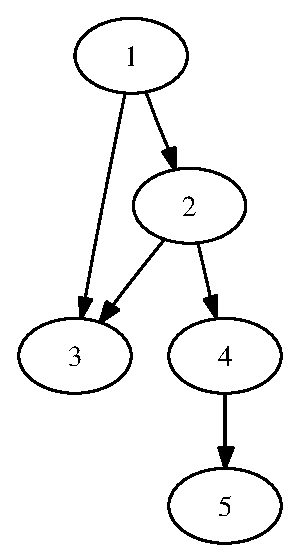
\epsfig{file=Figures/graph0,scale=0.6}

  \caption{A simple graph.}
  \label{fig:graph0}
\end{figure}



\noindent
The graph given by the relation \texttt{R} contains only the direct connections of vertices.  For example, in
the graph shown in Figure \ref{fig:graph0}, there is a direct connection from vertex $1$ to vertex $2$ and
another direct connection from vertex $2$ to vertex $4$.  Intuitively, vertex $4$ is reachable from vertex $1$,
since from vertex $1$ we can first reach vertex $2$ and from vertex $2$ we can then reach vertex $4$.  However,
there is is no direct connection between the vertices $1$ and $4$.  To make this more formal, define
a \blue{path} of a graph $R$ as a list of vertices
\\[0.2cm]
\hspace*{1.3cm}
$[x_1, x_2, \cdots, x_n]$ \quad such that \quad $\pair(x_i,x_{i+1}) \in R$ \quad for all $i=1,\cdots,n-1$.
\\[0.2cm]
In this case, the path $[x_1, x_2, \cdots, x_n]$ is written as
\\[0.2cm]
\hspace*{1.3cm}
$x_1 \mapsto x_2 \mapsto \cdots \mapsto x_n$
\\[0.2cm]
and has the \blue{length} $n-1$, since there are $n-1$ direct connections of the form $\pair(x_i,x_{i+1})$ that
make up this path.
To put it differently,  the length of a path
$[x_1,x_2,\cdots,x_n]$ is defined as the number of edges connecting the vertices and not as the
number of vertices appearing on the path.

Furthermore,  two vertices $a$ and $b$ of a graph are said to be \blue{connected} iff there exists a path
\\[0.2cm]
\hspace*{1.3cm}
$[x_1,\cdots,x_n]$ \quad such that \quad $a = x_1$ \quad and \quad $b = x_n$.
\\[0.2cm]
The goal of this section is to develop an algorithm that checks whether two vertices $a$ and $b$ are connected.
Furthermore, we want to be able to compute the corresponding path connecting the vertices $a$ and $b$.


\subsection{Computing the Transitive Closure of a Relation}
We have already noted that a graph can be represented as the set of its edges and hence as a \blue{binary relation}.
We have previously defined a \blue{binary relation} as a set of pairs.  We also need the notion of a \blue{relational product}:
If $Q$ and $R$ are binary relations, then the \blue{relational product} $Q \circ R$ of $Q$ and $R$ is defined as
\\[0.2cm]
\hspace*{1.3cm}
$Q \circ R := \Bigl\{ \pair(x, z) \Bigm| \exists y:\bigl(\pair(x,y) \in Q \wedge \pair(y,z) \in R\bigr) \Bigr\}$.
\\[0.2cm]
Furthermore, for any $n \in \mathbb{N}^*$ we can define the $n$-th power $R^n$ of the relation $R$ by induction.
\begin{description}
\item[Base Case:] $n = 1$.

             $R^1 := R$
\item[Induction Step:] $n \mapsto n+1$ 

             $R^{n+1} := R^n \circ R$.
\end{description}
The idea behind this definition is that if $\pair(x, z) \in R^n$, then there is a path of length $n$ that
starts in $x$ and ends in $z$.

In order to decide whether there is a path connecting two vertices we have to compute the 
\href{https://en.wikipedia.org/wiki/Transitive_closure}{transitive closure} $R^+$ of a relation $R$.  
To understand this notion, we first need to define the concept of \blue{transitivity}:  A relation $R$ is
transitive if and only if the following holds:
\\[0.2cm]
\hspace*{1.3cm}
$\pair(x,y) \in T \wedge \pair(y, z) \in T \rightarrow \pair(x, z) \in T$ \quad for all $x,y,z$. 
\\[0.2cm]
Now the \blue{transitive closure} $R^+$ of a binary relation $R$ is the \blue{smallest} relation $T$ such that the following
conditions hold:
\begin{itemize}
\item $R$ is a subset of $T$, i.e. we have $R \subseteq T$.
\item $T$ is transitive.
\end{itemize}
The lecture on
\href{https://github.com/karlstroetmann/Lineare-Algebra/blob/master/Skript/lineare-algebra.pdf}{Lineare Algebra} 
gives a prove that the transitive closure $R^+$ of a binary relation can be computed as follows:
\\[0.2cm]
\hspace*{1.3cm}
$R^+ = \bigcup\limits_{n=1}^{\infty} R^n = R^1 \cup R^2 \cup R^3 \cup \cdots$  
\\[0.2cm]
Initially, this formula might look intimidating as it suggests an infinite computation.
Fortunately, it turns out that we do not have to compute the powers $R^n$ for every $n \in \mathbb{N}$.  Let me
explain the reason that allows us to cut the computation short.  
\begin{enumerate}
\item $R$ is the set of direct connections between two vertices.
\item $R^2$ is the same as $R \circ R$ and this relational product is defined as
      \\[0.2cm]
      \hspace*{1.3cm}
       $R \circ R = \bigl\{ \pair(x,z) \bigm| \exists y \colon(\pair(x,y) \in R \wedge \pair(y,z)) \in R \bigr\}$.
      \\[0.2cm]
      Hence, $R \circ R$ contains those pairs $\pair(x,z)$ that are connected via one intermediate vertex $y$,
      i.e.~there is a path of the form $x \mapsto y \mapsto z$ that connects $x$ and $z$.  This path
      has length 2.  In general, we can show by induction on $n$ that $R^n$ connect those pairs that are
      connected by a path of length $n$.  The induction step of this proof runs as follows:

      $R^{n+1}$ is defined as $R^n \circ R$ and therefore we have
      \\[0.2cm]
      \hspace*{1.3cm}
      $R^n \circ R = \{ \pair(x,z) \mid \exists y \colon \pair(x,y) \in R^n \wedge \pair(y,z) \in R \}$.
      \\[0.2cm]
      As $\pair(x,y) \in R^n$, the induction hypothesis guarantees that the vertices $x$ and $y$ are
      connected by a path of length $n$.  Hence, this 
      path has the form
      \\[0.2cm]
      \hspace*{1.3cm}
      $\underbrace{x \mapsto \cdots \mapsto y}_{\mbox{\scriptsize path of length $n$.}}$
      \\[0.2cm]
      Adding $z$ at the end of this path will produce the path
      \\[0.2cm]
      \hspace*{1.3cm}
      $\underbrace{\underbrace{x \mapsto \cdots \mapsto y}_{\mbox{\scriptsize path of length $n$.}} \mapsto z}_{\mbox{\scriptsize path of length $n+1$.}}$.
      \\[0.2cm]
      This path has a length of $n + 1$ and, furthermore, connects $x$ and $z$.  Hence $R^{n+1}$
      contains those pairs $\pair(x, z)$ that are connected by a path of length $n+1$.
\end{enumerate}
Now the important observation is the following. The set of all vertices is finite.  For the arguments sake, let
us assume there are $k$ different vertices.  But then every path that has a length of $k$ or greater must
contain at least one vertex that is visited more than once and hence this path is longer than necessary,
i.e.~there is a shorter path that connects the same vertices.  Therefore, for a finite graph with $k$ vertices,
the formula to compute the transitive closure can be simplified as follows:
\\[0.2cm]
\hspace*{1.3cm} 
$\ds R^+ = \bigcup\limits_{i=1}^{k-1} R^i$.
\\[0.2cm]
While we could use this formula as its stands, it is more efficient to use a \blue{fixed-point iteration} instead.
To this end, we prove that the transitive closure $R^+$ satisfies the following equation:
\begin{equation}
  \label{fixpunkt}
  R^+ = R \cup R^+ \circ R. 
\end{equation}
The precedence of the operator $\circ$ 
is higher than the precedence of the operator $\cup$.  Therefore, the expression $R \cup R^+ \circ R$ is
equivalent to the expression $R \cup (R^+ \circ R)$.  In order to prove equation \ref{fixpunkt} we first note
that the following  \blue{law of distributivity} holds:
\\[0.2cm]
\hspace*{1.3cm}
$\ds (P \cup Q) \circ R = (P \circ R) \cup (Q \circ R)$.
\\[0.2cm]
(A proof of this equation can be found in my lecture notes on
\href{https://github.com/karlstroetmann/Lineare-Algebra/blob/master/Skript/lineare-algebra.pdf}{linear algebra}
on page 42.)  Using this law, we can prove equation \ref{fixpunkt} algebraically.  We have:
\\[0.2cm]
\hspace*{1.3cm}
$
\begin{array}{cll}
    & R \cup R^+ \circ R \\[0.2cm]
  = & R \cup \Bigl(\bigcup\limits_{i=1}^{\infty} R^i \Bigr) \circ R \\[0.4cm]
  = & R \cup \bigl(R^1 \cup R^2 \cup R^3 \cup \cdots \bigr) \circ R \\[0.2cm]
  = & R \cup \bigl(R^1 \circ R \cup R^2 \circ R \cup R^3 \circ R \cup \cdots \bigr) \\[0.2cm]
  = & R \cup \bigl(R^2 \cup R^3 \cup  R^4 \cup \cdots \bigr)  \\[0.2cm]
  = & R^1 \cup R^2 \cup R^3 \cup  R^4 \cup \cdots  \\[0.2cm]
  = & \bigcup\limits_{i=1}^{\infty} R^i \\[0.4cm]
  = & R^+.
\end{array}
$
\\[0.2cm]
Equation  \ref{fixpunkt} can now be used to compute $R^+$ via a fixed-point iteration.
To this end, let us define a sequence of relations $(T_n)_{n \in \mathbb{N}}$ by induction on $n$:
\begin{enumerate}
\item[I.A.] $n = 0$: 

            $T_0 = R$
\item[I.S.] $n \mapsto n+1$:

            $T_{n+1} = R \cup T_n \circ R $. 
\end{enumerate}
The relation  $T_n$ can be expressed via the relation $R$, we have
\begin{enumerate}
\item $T_0 = R$.
\item $T_1 = R \cup T_0 \circ R = R \cup R \circ R = R^1 \cup R^2$.
\item$\begin{array}[t]{lcl}
       T_2  & = & R \cup T_1 \circ R \\
            & = & R \cup (R^1 \cup R^2) \circ R \\
            & = & R^1 \cup R^2 \cup R^3. \\
       \end{array}
      $
\end{enumerate}
In general, we can show by induction that
\\[0.2cm]
\hspace*{1.3cm}
$\ds T_n = \bigcup\limits_{i=1}^{n+1} R^i$
\\[0.2cm]
holds for all $n \in \mathbb{N}$.  As $R^1 = R$, the base case $n=0$ of this proof is immediate from the definition of $T_0$.
In the induction step we observe the following:
\\[0.2cm]
\hspace*{1.3cm}
$
 \begin{array}{lcll}
   T_{n+1} & = & \ds R \cup T_n \circ R & \mbox{(by definition)} \\[0.2cm]
           & = & \ds R \cup \biggl(\bigcup\limits_{i=1}^{n+1} R^i\biggr) \circ R &
                 \mbox{(by induction hypothesis)} \\[0.4cm]
           & = & \ds R \cup \left(R \cup \cdots \cup R^{n+1}\right) \circ R \\[0.2cm] 
           & = & \ds R^1 \cup R^2 \cup \cdots \cup R^{n+2}  &
                 \mbox{(by the distributivity of $\circ$ over $\cup$)} \\[0.2cm]
           & = & \ds \bigcup\limits_{i=1}^{n+2} R^i & \Box 
   \end{array}
$
\\[0.2cm]
The sequence $(T_n)_{n\in\mathbb{N}}$ has another useful property:  It is 
\blue{monotonically increasing}.  In general, a sequence of sets $(X_n)_{n\in\mathbb{N}}$ is called
\blue{monotonically increasing} iff we have
\\[0.2cm]
\hspace*{1.3cm}
$\forall n \in \mathbb{N}: X_n \subseteq X_{n+1}$,
\\[0.2cm]
i.e.~the sets $X_n$ get bigger with growing index $n$.
The monotonicity of the sequence  $(T_n)_{n \in \mathbb{N}}$ is an immediate consequence of the equation
\\[0.2cm]
\hspace*{1.3cm}
$\ds T_n = \bigcup\limits_{i=1}^{n+1} R^i$ 
\\[0.2cm]
because we have:
\\[0.2cm]
\hspace*{1.3cm}
$
\begin{array}[t]{llcl}
                & \ds T_n \subseteq T_{n+1} \\[0.2cm]
\Leftrightarrow & \ds \bigcup\limits_{i=1}^{n+1} R^i \subseteq \bigcup\limits_{i=1}^{n+2} R^i \\[0.5cm]
\Leftrightarrow & \ds \bigcup\limits_{i=1}^{n+1} R^i \subseteq \left(\bigcup\limits_{i=1}^{n+1} R^i\right) \cup R^{n+2} \\
\end{array}
$
\\[0.2cm]
If the relation  $R$ is finite, then the transitive closure $R^+$ is finite, too.  All of the sets $T_n$ 
are subsets of $R^+$ because we have
\\[0.2cm]
\hspace*{1.3cm}
$\ds T_n = \bigcup\limits_{i=1}^{n+1} R^i \subseteq \bigcup\limits_{i=1}^{\infty} R^i = R^+$ \quad for all $n \in \mathbb{N}$.
\\[0.2cm]
Hence the sets $T_n$ can not grow indefinitely.  Because of the monotonicity of the sequence 
$(T_n)_{n\in\mathbb{N}}$ it follows that there exists an index  $k \in \mathbb{N}$ such that the sets $T_n$ do
not grow any further once $n$ has reached $k$, i.e.~we have
\\[0.2cm]
\hspace*{1.3cm}
$\ds \forall n \in \mathbb{N}:( n \geq k \rightarrow T_n = T_k)$.
\\[0.2cm]
But this implies that
\\[0.2cm]
\hspace*{1.3cm}
$\ds T_n = \bigcup\limits_{i=1}^{n+1} R^i = \bigcup\limits_{i=1}^{\infty} R^i = R^+$ 
\quad holds for all $n \geq k$.
\\[0.2cm]
Therefore, the algorithm for computing  $R^+$ iterates the equation 
\\[0.2cm]
\hspace*{1.3cm}
$\ds T_{n+1} = R \cup T_n \circ R$
\\[0.2cm]
until the equation  $T_{n+1} = T_n$ is satisfied, since this implies that $T_n = R^+$.


\begin{figure}[!ht]
  \centering
\begin{Verbatim}[ frame         = lines, 
                  framesep      = 0.3cm, 
                  labelposition = bottomline,
                  numbers       = left,
                  numbersep     = -0.2cm,
                  xleftmargin   = 0.8cm,
                  xrightmargin  = 0.8cm,
                ]
    def product(R1, R2):
        'Compute the relational product of R1 and R2.'
        return { (x, z) for (x, y1) in R1 for (y2, z) in R2 if y1 == y2 }
    
    def transClosure(R):
        'Compute the transitive closure of the binary relation R.'
        T = R
        while True:
            oldT = T
            T    = product(R,T) | R
            if T == oldT:
                return T
    
    R = { (1,2), (2,3), (1,3), (2,4), (4,5) }
    print( 'R  = ', R );
    print( 'Computing the transitive closure of R:' );
    T = transClosure(R);
    print( 'R+ = ', T );
\end{Verbatim} 
\vspace*{-0.3cm}
\caption{Computing the transitive closure.}  
\label{fig:transitive-closure.py}
\end{figure} %\$

\noindent
The program 
\href{https://github.com/karlstroetmann/Logic/blob/master/Python/transitive-closure.py}{\texttt{transitive-closure.py}}
that is shown in Figure
\ref{fig:transitive-closure.py} on page \pageref{fig:transitive-closure.py} shows an implementation of this idea.
The program produces the following output:
\begin{verbatim}
    R  = {(1, 2), (1, 3), (4, 5), (2, 3), (2, 4)}
    Computing the transitive closure of R:
    R+ = {(1, 2), (1, 3), (4, 5), (1, 4), (1, 5), (2, 3), (2, 5), (2, 4)}
\end{verbatim}
The transitive closure $R^+$ of a relation $R$ has a very intuitive interpretation:
It contains all pairs $\pair(x,y)$ such that there is a path leading from 
$x$ to $y$.  
The function $\texttt{product}(R_1, R_2)$ computes the relational product $R_1\circ R_2$ 
according to the formula
\\[0.2cm]
\hspace*{1.3cm}
$R_1 \circ R_2 = \Bigl\{ \langle x, z \rangle \Bigm| \exists y:\bigl(\pair(x,y) \in R_1 \wedge \pair(y,z) \in R_2\bigr) \Bigr\}$.


\subsection{Computing the Paths}
So far, given a graph represented by a relation $R$ and two vertices $x$ and $y$, we can only check
whether there is a path leading from $x$ to $y$, but we cannot compute this path.  In this
subsection we will extend the procedure \texttt{transClosure} so that it will also compute the
corresponding path.  The main idea is to extend the notion of a relational product to the notion of
a \blue{path product}, where a \blue{path product} is defined on sets of paths.  In order to do so,
we introduce three functions for tuples.
\begin{enumerate}
\item Given a tuple $T$, the function $\texttt{first}(T)$ returns the first element of $T$: 
      \\[0.2cm]
      \hspace*{1.3cm}
      $\texttt{first}\bigl(\langle x_1,\cdots,x_m\rangle\bigr) = x_1$.
\item Given a tuple $T$, the function $\texttt{last}(T)$ returns the last element of $T$: 
      \\[0.2cm]
      \hspace*{1.3cm}
      $\texttt{last}\bigl(\langle x_1,\cdots,x_m\rangle\bigl) = x_m$.
\item If $S = \langle x_1, \cdots, x_m\rangle$ and $T = \langle y_1, \cdots, y_n \rangle$ are two tuples  such that
      $\texttt{first}(S) = \texttt{last}(S)$, we define the \blue{join} $S \oplus T$ of $S$ and $T$ as \\[0.2cm]
      \hspace*{1.3cm}
      $S \oplus T = \langle x_1, \cdots, x_m, y_2, \cdots, y_n \rangle$.
\end{enumerate}
If $\mathcal{P}_1$ and $\mathcal{P}_2$ are sets of tuples representing paths, we define the \blue{path product} of
$\mathcal{P}_1$ and $\mathcal{P}_2$ as follows: \\[0.2cm]
\hspace*{1.3cm} 
$\mathcal{P}_1 \bullet \mathcal{P}_2 = 
\bigl\{\; T_1 \oplus T_2 \mid T_1 \in \mathcal{P}_1 \wedge T_2 \in \mathcal{P}_2 \wedge \texttt{last}(T_1) = \texttt{first}(T_2) \;\bigr\}
$.

\begin{figure}[!ht]
  \centering
\begin{Verbatim}[ frame         = lines, 
                  framesep      = 0.3cm, 
                  labelposition = bottomline,
                  numbers       = left,
                  numbersep     = -0.2cm,
                  xleftmargin   = 0.8cm,
                  xrightmargin  = 0.8cm,
                ]
    def findPaths(R):
        P = R;
        while True:
            oldP = P
            P    = R | pathProduct(P, R)
            if P == oldP:
                return P

    def pathProduct(P, Q):
        return { join(S, T) for S in P for T in Q if S[-1] == T[0] }
    
    def join(S, T):
        return S + T[1:]
    
    R = { (1,2), (2,3), (1,3), (2,4), (4,5) }
    print('R = ', R)
    print('Computing all paths:' )
    P = findPaths(R)
    print('P = ', P)
\end{Verbatim} 
\vspace*{-0.3cm}
\caption{Computing all connections.}  \label{fig:path.py}
\end{figure} %\$

\begin{figure}[!ht]
  \centering
  \vspace*{-9cm}

  \epsfig{file=Figures/graph-zykl,scale=0.5}
  \vspace*{-1cm}

  \caption{A graph with a cycle.}
  \label{fig:graph-zykl}
\end{figure}

Using the notion of a \blue{path product} we are able to extend the program shown in Figure
\ref{fig:transitive-closure.py} such that it computes all paths between two vertices.
The resulting program
\href{https://github.com/karlstroetmann/Logic/blob/master/Python/path.py}{\texttt{path.py}}
is shown in Figure \ref{fig:path.py} on page \pageref{fig:path.py}.
Unfortunately, the program does not work any more if the graph is \blue{cyclic}.  A graph is defined
to be \blue{cyclic} if there is a path of length greater than $1$ that starts and ends at the same
vertex.  This path is then called a \blue{cycle}.
Figure \ref{fig:graph-zykl} on page \pageref{fig:graph-zykl} shows a cyclic graph.  This graph is
cyclic because it contains the path
\\[0.2cm]
\hspace*{1.3cm}
$\langle 1, 2, 4, 1 \rangle$
\\[0.2cm]
and this path is a cycle.
The problem with this graph is that it contains an infinite number of paths that connect the vertex
1 with the vertex 2: \\[0.2cm]
\hspace*{1.3cm}
$\langle 1, 2 \rangle$, $\langle 1, 2, 4, 1, 2 \rangle$, 
$\langle 1, 2, 4, 1, 2, 4, 1, 2 \rangle$, 
$\langle 1, 2, 4, 1, 2, 4, 1, 2, 4, 1, 2 \rangle$, $\cdots$
\\[0.2cm]
Of course, there is no point in computing a path that visits a vertex more than once as these paths
contain cycles.  Our goal is to eliminate all those paths that contain cycles.


\begin{figure}[!ht]
  \centering
\begin{Verbatim}[ numbers       = left,
                  numbersep     = -0.2cm,
                  frame         = lines, 
                  framesep      = 0.3cm, 
                  labelposition = bottomline,
                  xleftmargin   = 0.0cm,
                  xrightmargin  = 0.0cm,
                ]
    def pathProduct(P, Q):
        return { join(S, T) for S in P for T in Q
                            if S[-1] == T[0] and noCycle(S, T)
               }
    
    def noCycle(T1, T2):
        return len({ x for x in T1 }.intersection({ x for x in T2 })) == 1
\end{Verbatim} 
\vspace*{-0.3cm}
\caption{Computing the connections in a cyclic graph.}  
\label{fig:path-cyclic.py}
\end{figure} %\$

Figure \ref{fig:path-cyclic.py} on page shows how the implementation of the function
\texttt{pathProduct} has to be changed so that the resulting program
\href{https://github.com/karlstroetmann/Logic/blob/master/Python/path-cyclic.py}{\texttt{path-cyclic.py}}
works also for cyclic graphs. 
\begin{enumerate}
\item In line 2 and 3, we compute only those paths that are not cyclic.
\item Line 6 defines a function \texttt{noCycle} that tests, whether the join  $\texttt{T1} \oplus \texttt{T2}$ is cyclic.  The join
      of \texttt{T1} and \texttt{T2} is cyclic iff the tuples \texttt{T1} and \texttt{T2} have more
      than one common element.  The tuples \texttt{T1} and \texttt{T2} will always have at least one common element, as we join
      these tuples only if the last element of \texttt{T1} is equal to the first element of  \texttt{T2}.
      If there would be an another vertex common to both \texttt{T1} and \texttt{T2}, then the path
      $\texttt{T1} \oplus \texttt{T2}$ would be cyclic.
\end{enumerate}

In general, we are not really interested to compute all possible paths between two given vertices
\texttt{x} and \texttt{y}.  Instead, we just want to compute the shortest path leading from \texttt{x} to \texttt{y}.
Figure \ref{fig:find_path.py} on page \pageref{fig:find_path.py} shows the procedure \texttt{reachable}. 
This procedure takes three arguments:
\begin{enumerate}
\item \texttt{start} and \texttt{goal} are vertices of a graph.
\item \texttt{R} is a binary relation representing a directed graph.
\end{enumerate}
The call  \texttt{reachable(start, goal, R)} checks whether \texttt{start} and \texttt{goal} are connected and, furthermore,
computes the shortest path from \texttt{start} to \texttt{goal}, provided such a path exists.
The complete program can be found in the file
\href{https://github.com/karlstroetmann/Logic/blob/master/Python/find\_path.py}{\texttt{find\_path.py}}.
Next, we discuss the implementation of the procedure  \texttt{reachable}.
\begin{enumerate}
\item Line 2 initializes the set \texttt{P}.  After $n$ iterations, this set will contain all paths
      that start with the vertex \texttt{start} and that have a length of at most $n$.

      Initially, there is just the trivial path $\langle\texttt{start}\rangle$ that starts with vertex
      \texttt{start} and has length $0$.
\item Line 5 tries to extend all previously computed paths by one step.
\item Line 6 selects all those paths from the set \texttt{P} that lead to the vertex \texttt{goal}.
      These paths are stored in the set \texttt{Found}.
\item Line 7 checks whether we have indeed found a path ending at \texttt{goal}.  This is the case if
      the set \texttt{Found} is not empty.  
      In this case, we return any of these paths.
\item If we have not yet found the vertex \texttt{goal} and, furthermore, we have not been able to find
      any new paths during this iteration,  the procedure returns in line 10.
      As the \texttt{return} statement in line 11 does not return a value, the procedure will
      instead return the value \texttt{None}.
\end{enumerate}
The procedure call \texttt{reachable(start,goal R)} will compute the \textbf{shortest} path connecting
\texttt{start} and \texttt{goal} because it computes path with increasing length.  The first iteration
computes all paths starting in \texttt{start} that have a length of at most 1, the second iteration
computes all paths starting in \texttt{start} that have a length of at most 2, and in general the $n$-th
iteration computes all paths starting in \texttt{start} that have a length of at most $n$.  Hence, if
there is a path of length $n$, then this path will be found in the $n$-iteration unless a shorter path has
already been found in a previous iteration.  

\remarkEng
The algorithm described above is known as 
\href{https://en.wikipedia.org/wiki/Breadth-first_search}{breadth first search}. \eox 

\begin{figure}[!ht]
  \centering
\begin{Verbatim}[ frame         = lines, 
                  framesep      = 0.3cm, 
                  labelposition = bottomline,
                  numbers       = left,
                  numbersep     = -0.2cm,
                  xleftmargin   = 0.8cm,
                  xrightmargin  = 0.8cm,
                ]
    def reachable(start, goal, R):
        P = { (start,) }
        while True:
            oldP  = P
            P     = P | path_product(P, R)
            Found = { T for T in P if T[-1] == goal }
            if Found != set():
                return Found.pop()
            if P == oldP:
                return
                
    def path_product(P, R):
        return set( add(T1, T2) for T1 in P for T2 in R
                             if T1[-1] == T2[0] and noCycle(T1, T2)
                  )
    
    def noCycle(T1, T2):
        return len(set(T1).intersection(set(T2))) == 1
    
    def add(T, P):
        return T + (P[-1],)
\end{Verbatim} 
\vspace*{-0.3cm}
\caption{Finding the shortest path between two vertices.}  
\label{fig:find_path.py}
\end{figure}

\subsection{The Wolf, the Goat, and the Cabbage}
Next, we present an application of the theory developed so far.  We solve a problem that has puzzled
the greatest agricultural economists for centuries.  The puzzle we want to solve is known as the 
\href{http://jeux.lulu.pagesperso-orange.fr/html/anglais/loupChe/loupChe1.htm}{wolf-goat-cabbage puzzle}:  
\vspace*{0.3cm}

\begin{minipage}[c]{16cm}
{\sl
An agricultural economist has to sell a wolf, a goat, and a cabbage on a market place.  In order to
reach the market place, she has to cross a river.  The boat that she can use is so small that it can
only accommodate either the goat, the wolf, or the cabbage in addition to the agricultural economist.
Now if the agricultural economist leaves the wolf alone with the goat, the wolf will eat the goat.
If, instead, the agricultural economist leaves the goat with the cabbage, the goat will eat the cabbage.
Is it possible for the agricultural economist to develop a schedule that allows her to cross the river
without either the goat or the cabbage being eaten?
}
\end{minipage}
\vspace*{0.3cm}

\noindent
In order to compute a schedule, we first have to model the problem.  The various \blue{states} of the problem will
be regarded as \blue{vertices} of a graph and this graph will be represented as a binary relation.
To this end we define the set
\begin{verbatim}
  All = {'farmer', 'wolf, 'goat', 'cabbage'}
\end{verbatim}
Every node will be represented as a subset \texttt{S} of the set \texttt{All}.  The idea is that the set \texttt{S}
specifies those objects that are on the left side of the river.  We assume that initially the farmer and his goods
are on the left side of the river. 
Therefore, the set of all possible states can be defined as the set
\begin{verbatim}
  States = {S for S in power(All) if not problem(S) and not problem(All-S)}
\end{verbatim}
Here, we have used the procedure \texttt{problem} to check whether a given set \texttt{S} has a problem. 
Note that since \texttt{S} is the set of objects on the left side, the expression $\texttt{All-S}$
computes the set of objects on the right side of the river.

Next, a set \texttt{S} of objects has a problem if both of the following conditions
are satisfied:
\begin{enumerate}
\item The farmer is not an element of \texttt{S} and
\item either \texttt{S} contains both the goat and the cabbage or \texttt{S} contains both the wolf and the goat.
\end{enumerate}
Therefore, we can implement the function \texttt{problem} as follows:
\begin{verbatim}
  def problem(S):
      return ('farmer' not in S) and             \
             (('goat' in S and 'cabbage' in S) or   # goat eats cabbage
              ('wolf' in S and 'goat'    in S)   )  # wolf eats goat
\end{verbatim}
We proceed to compute the relation \texttt{R} that contains all possible transitions between
different states.  We will compute \texttt{R} using the formula:
\\[0.2cm]
\hspace*{0.75cm}
\texttt{R = R1 + R2;}
\\[0.2cm]
Here \texttt{R1} describes the transitions that result from the farmer crossing the river from left
to right, while \texttt{R2} describes the transitions that result from the farmer crossing the river
from right to left.  We can define the relation \texttt{R1} as follows:
\begin{verbatim}
  R1 = { (S, S-B) for S in States for B in power(S)
                  if S-B in States and 'farmer' in B and len(B) <= 2
       }
\end{verbatim}
Let us explain this definition in detail:
\begin{enumerate}
\item Initially, \texttt{S} is the set of objects on the left side of the river.  Hence, \texttt{S}
      is an element of the set of all states that we have defined as \texttt{P}.
\item \texttt{B} is the set of objects that are put into the boat and that do cross the river.  Of
      course, for an object to go into the boat is has to be on the left side of the river to begin
      with.  Therefore, \texttt{B} is a subset of \texttt{S} and hence an element of the power set
      of \texttt{S}. 
\item Then  \texttt{S-B} is the set of objects that are left on the left side of the river after
      the boat has crossed.  Of course, the new state \texttt{S-B} has to be a state that does not
      have a problem.  Therefore, we check that \texttt{S-B} is an element of \texttt{States}.
\item Furthermore, the farmer has to be inside the boat.  This explains the condition 
      \\[0.2cm]
      \hspace*{1.3cm}
      \texttt{\symbol{39}farmer\symbol{39} in B}.
\item Finally, the boat can only have two passengers.  Therefore, we have added the condition
      \\[0.2cm]
      \hspace*{1.3cm}
      \texttt{len(B) <= 2}.
\end{enumerate}
Next, we have to define the relation \texttt{R2}.  However, as crossing the river from right to left
is just the reverse of crossing the river from left to right, \texttt{R2} is just the \blue{inverse} of
\texttt{R1}.   Hence we define:
\begin{verbatim}
  R2 = { (S2, S1) for (S1, S2) in R1 }
\end{verbatim}
Next, the relation \texttt{R} is the union of \texttt{R1} and \texttt{R2}:
\begin{verbatim}
  R = R1 | R2
\end{verbatim}
Finally, the start state has all objects on the left side.  Therefore, we have
\begin{verbatim}
  start = All
\end{verbatim}
In the end, all objects have to be on the right side of the river.  That means that nothing is left
on the left side.  Therefore, we define
\begin{verbatim}
  goal = {}
\end{verbatim}


\begin{figure}[h]
  \centering

  \epsfig{file=Figures/wolf-goat-cabbage, scale=0.4}

  \caption{The relation \texttt{R} shown as a directed graph.}
  \label{fig:wolf-goat-cabbage.pdf}
\end{figure}




Figure \ref{fig:wolf-ziege} on page \pageref{fig:wolf-ziege} shows the program
\href{https://github.com/karlstroetmann/Logic/blob/master/Python/wolf-goat-cabbage.py}{\texttt{wolf-goat-cabbage.py}}
that combines the statements shown so far.  The solution computed by this program is shown in Figure
 \ref{fig:wolf-ziege-solution}.

\begin{figure}[!ht]
  \centering
\begin{Verbatim}[ codes         = {\catcode`$=3\catcode`_=8\catcode`^=7},
                  frame         = lines, 
                  framesep      = 0.3cm, 
                  labelposition = bottomline,
                  numbers       = left,
                  numbersep     = -0.2cm,
                  xleftmargin   = 0.3cm,
                  xrightmargin  = 0.3cm,
                ]
    def problem(S):
        return ('farmer' not in S) and             \
               (('goat' in S and 'cabbage' in S) or   # goat eats cabbage
                ('wolf' in S and 'goat'    in S)   )  # wolf eats goat
    
    All   = frozenset( {'farmer', 'wolf', 'goat', 'cabbage'} )
    R1    = { (S, S - B) for S in States for B in power(S)
                         if S - B in States and 'farmer' in B and len(B) <= 2
            }
    R2    = { (S2, S1) for (S1, S2) in R1 }
    R     = R1 | R2
    start = All
    goal  = frozenset()
    Path  = findPath(start, goal, R)
\end{Verbatim} 
\vspace*{-0.3cm}
\caption{Solving the wolf-goat-cabbage problem.}  
\label{fig:wolf-ziege}
\end{figure}


\begin{figure}[!ht]
  \centering
\begin{Verbatim}[ codes         = {\catcode`$=3\catcode`_=8\catcode`^=7},
                  frame         = lines, 
                  framesep      = 0.3cm, 
                  labelposition = bottomline,
                  numbers       = left,
                  numbersep     = -0.2cm,
                  xleftmargin   = 0.8cm,
                  xrightmargin  = 0.8cm,
                ]
    {'cabbage', 'farmer', 'goat', 'wolf'}                                 {}
                             >>>> {'farmer', 'goat'} >>>> 
    {'cabbage', 'wolf'}                                   {'farmer', 'goat'}
                             <<<< {'farmer'} <<<< 
    {'cabbage', 'farmer', 'wolf'}                                   {'goat'}
                             >>>> {'farmer', 'wolf'} >>>> 
    {'cabbage'}                                   {'farmer', 'goat', 'wolf'}
                             <<<< {'farmer', 'goat'} <<<< 
    {'cabbage', 'farmer', 'goat'}                                   {'wolf'}
                             >>>> {'cabbage', 'farmer'} >>>> 
    {'goat'}                                   {'cabbage', 'farmer', 'wolf'}
                             <<<< {'farmer'} <<<< 
    {'farmer', 'goat'}                                   {'cabbage', 'wolf'}
                             >>>> {'farmer', 'goat'} >>>> 
    {}                                 {'cabbage', 'farmer', 'goat', 'wolf'}
\end{Verbatim} 
\vspace*{-0.3cm}
\caption{A schedule for the agricultural economist.}  
\label{fig:wolf-ziege-solution}
\end{figure}
\pagebreak
\vspace*{\fill}



\section{Symbolic Differentiation}
In this section we will develop a program that reads an arithmetic expression like 
\\[0.2cm]
\hspace*{1.3cm}
\texttt{\symbol{34}x * exp(x)\symbol{34}},
\\[0.2cm]
interprets this string as describing the real valued function 
\\[0.2cm]
\hspace*{1.3cm}
$x \mapsto x \cdot \exp(x)$, 
\\[0.2cm]
and then takes the derivative of this function with respect to the variable $x$.  In order to specify the input
of this program more clearly, we first define the notion of an \blue{arithmetic expression} inductively.
\begin{enumerate}
\item Every number $c \in \mathbb{R}$ is an arithmetic expression.
\item Every variable $v$ is an arithmetic expression.
\item If $s$ and $t$ are arithmetic expressions, then
      \\[0.2cm]
      \hspace*{1.3cm}
      $s + t$, \quad $s - t$, \quad $s * t$, \quad $s / t$, \quad and \quad $s \,\mathtt{**}\, t$
      \\[0.2cm]
      are arithmetic expressions.  Here $s \,\mathtt{**}\, t$ is interpreted as $s^t$.
      
\item If $e$ is an arithmetic expression, then both
      \\[0.2cm]
      \hspace*{1.3cm}
      $\exp(e)$ \quad and \quad $\ln(e)$
      \\[0.2cm]
      are arithmetic expressions.
\end{enumerate}
We want do implement a function \texttt{diff} that takes two arguments:
\begin{enumerate}
\item The first argument \texttt{expr} is an arithmetic expression.
\item The second argument \texttt{var} is the name of a variable.
\end{enumerate}
The function call \texttt{diff(expr, var)} will then compute the derivative of \texttt{expr} with respect to the variable \texttt{var}.  For example, the function call \texttt{diff(\symbol{34}x*exp(x)\symbol{34}, \symbol{34}x\symbol{34})} will compute the output
\\[0.2cm]
\hspace*{1.3cm}
\symbol{34}\texttt{1*exp(x) + x*exp(x)}\symbol{34}
\\[0.2cm]
because we have:
$$ \frac{\mathrm{d}\;}{\mathrm{d}x} \bigl( x \cdot \mathrm{e}^x \bigr) = 1 \cdot x + x \cdot \mathrm{e}^x $$
It would be very tedious to \blue{represent} arithmetic expressions as strings.  Instead, we will represent
arithmetic expressions as \blue{nested tuples}.  The notion of a \emph{nested tuple} is defined inductively:
\begin{itemize}
\item $\langle x_1, x_2, \cdots, x_n \rangle$ is a nested tuple if each of the components $x_i$ is either a
      number, a string, or is itself a nested tuple.
\end{itemize}
For example, the arithmetic expression ``\texttt{x*exp(x)}'' is represented as the nested tuple
\\[0.2cm]
\hspace*{1.3cm}
$\bigl\langle\texttt{\symbol{34}}*\texttt{\symbol{34}}, \texttt{\symbol{34}}x\texttt{\symbol{34}}, \langle \texttt{\symbol{34}}\mathtt{exp}\texttt{\symbol{34}}, \texttt{\symbol{34}}x\texttt{\symbol{34}} \rangle\bigr\rangle$.
\\[0.2cm]
In order to be able to convert string into nested tuples, we need a \blue{parser}.  A parser is a program that
takes a string as input and transforms this string into a nested tuple, which is then returned as a result.
I have implemented a parser in the file ``\texttt{exprParser.py}''.  The details of the implementation of this
parser will be discussed in the lecture on algorithms.

\noindent
The function \texttt{diff} that is shown in Figure \ref{fig:diff.py} on page \pageref{fig:diff.py} is part
of the program
\href{https://github.com/karlstroetmann/Logic/blob/master/Python/diff.py}{\texttt{diff.py}}.
This function is called with one argument:
The argument \texttt{e} is an arithmetic expression.
The function \texttt{diff} interprets its argument \texttt{e} as a function of the variable
\texttt{x}.  We take the \href{https://en.wikipedia.org/wiki/Derivative}{derivative} of this
function with respect to the variable \texttt{x}.  For example, in order to compute the derivative of
the function
\\[0.2cm]
\hspace*{1.3cm}
$x \mapsto x^x$,
\\[0.2cm]
we can call the function  \texttt{diff} as follows:
\\[0.2cm]
\hspace*{1.3cm}
\texttt{diff(\symbol{34}x ** x\symbol{34})}.
\\[0.2cm]
Let us now discuss the implementation of the function \texttt{diff} in more detail.  
\begin{enumerate}
\item The lines 3 - 6 implement the rule: 
      $$\frac{\mathrm{d}\;}{\mathrm{d}x}\bigl(f(x) + g(x)\bigr) = \frac{\mathrm{d}\;}{\mathrm{d}x} f(x) + \frac{\mathrm{d}\;}{\mathrm{d}x} g(x)$$
\item Line 7 - 10 implement the rule:
      $$\frac{\mathrm{d}\;}{\mathrm{d}x}\bigl(f(x) - g(x)\bigr) = \frac{\mathrm{d}\;}{\mathrm{d}x} f(x) - \frac{\mathrm{d}\;}{\mathrm{d}x} g(x)$$      
\item Line 11 - 14 deals with the case where \texttt{e} is a product.  The 
      \href{https://en.wikipedia.org/wiki/Product\_rule}{product rule} is      
      $$ \frac{\mathrm{d}\;}{\mathrm{d}x}\bigl(f(x) \cdot g(x)\bigr) = \left(\frac{\mathrm{d}\;}{\mathrm{d}x} f(x)\right)\cdot g(x) + f(x) \cdot \left(\frac{\mathrm{d}\;}{\mathrm{d}x} g(x)\right)
      $$
\item Line 15 - 17 deals with the case where \texttt{e} is a quotient.  The
      \href{https://en.wikipedia.org/wiki/Quotient\_rule}{quotient rule} is
      $$ \frac{\mathrm{d}\;}{\mathrm{d}x}\left(\frac{f(x)}{g(x)}\right) = 
         \frac{\displaystyle\left(\frac{\mathrm{d}\;}{\mathrm{d}x} f(x)\right)\cdot g(x) - 
         f(x) \cdot \left(\frac{\mathrm{d}\;}{\mathrm{d}x} g(x)\right)}{g(x) \cdot g(x)}
      $$      
\item Line 19 - 21 deals with the case where \texttt{e} is a power.  Now in order to take the derivative of an
      expression of the form
      $$  f(x)^{g(x)} $$
      we first need to rewrite this expression using the following trick:
      $$ f(x)^{g(x)} = \exp\bigl(\ln\bigl(f(x)^{g(x)}\bigr)\bigr) = \exp\bigl(g(x) \cdot \ln(f(x))\bigr) $$
      Then, we can recursively call \texttt{diff} for this expression.  This works, because the function
      \texttt{diff} can deal with both the exponential function $x \mapsto \exp(x)$ and with the natural
      logarithm $x \mapsto \ln(x)$.  This rewriting is done in line 21.      
\item Line 22-25 deals with the case where \texttt{e} has the form 
      $$\ln\bigl(f(x)\bigr)$$  
      In order to take the derivative of this expression, we first need to know the derivative of the natural
      logarithm.  This derivative is given as     
      $$ \frac{\mathrm{d}\;}{\mathrm{d}x} \ln(x) = \frac{1}{x}$$
      Then, using the \href{https://en.wikipedia.org/wiki/Chain\_rule}{chain rule} we have that
      $$ \frac{\mathrm{d}\;}{\mathrm{d}x} \ln\bigl(f(x)\bigr) = \frac{\frac{\mathrm{d}\;}{\mathrm{d}x} f(x)}{f(x)}$$     
\item Line 26 - 29 deals with the case where \texttt{e} has the form $\exp\bigl(f(x)\bigr)$.  
      In order to take the derivative of this expression, we first need to know the derivative of the 
      \href{https://en.wikipedia.org/wiki/Exponential\_function}{exponential function}.  
      This derivative is given as 
      $$ \frac{\mathrm{d}\;}{\mathrm{d}x} \exp(x) = \exp(x)$$    
      Then, using the \href{https://en.wikipedia.org/wiki/Chain\_rule}{chain rule} we have that
      $$\frac{\mathrm{d}\;}{\mathrm{d}x} \exp\bigl(f(x)\bigr) = \left(\frac{\mathrm{d}\;}{\mathrm{d}x} f(x)\right) \cdot \exp\bigl(f(x)\bigr) $$
\item Line 30-31 deals with the case where \texttt{e} is a variable and happens to be the same variable as
      \texttt{x}.  This is checked using the condition    
      \texttt{e == x}.  As we have
      $$\frac{\mathrm{d}x}{\mathrm{d}x} = 1,$$
      the function \texttt{diff} returns \texttt{1} in this case.  
\item Otherwise, the expression is assumed to be a constant and hence we return 0.
\end{enumerate}


\begin{figure}[!ht]
\centering
\begin{Verbatim}[ frame         = lines, 
                  framesep      = 0.3cm, 
                  firstnumber   = 1,
                  labelposition = bottomline,
                  numbers       = left,
                  numbersep     = -0.2cm,
                  xleftmargin   = 0.8cm,
                  xrightmargin  = 0.8cm,
                ]
    def diff(e):
        'differentiate the expressions e with respect to the variable x'
        if e[0] == '+':
            f , g  = e[1:]
            fs, gs = diff(f), diff(g)
            return ('+', fs, gs)
        if e[0] == '-':
            f , g  = e[1:]
            fs, gs = diff(f), diff(g)
            return ('-', fs, gs)
        if e[0] == '*':
            f , g  = e[1:]
            fs, gs = diff(f), diff(g)
            return ('+', ('*', fs, g), ('*', f, gs))
        if e[0] == '/':
            f , g  = e[1:]
            fs, gs = diff(f), diff(g)
            return ('/', ('-', ('*', fs, g), ('*', f, gs)), ('*', g, g))
        if e[0] == '**':
            f , g  = e[1:]
            return diff(('exp', ('*', g, ('ln', f))))
        if e[0] == 'ln':
            f  = e[1]
            fs = diff(f) 
            return ('/', fs, f)
        if e[0] == 'exp':
            f  = e[1]
            fs = diff(f) 
            return ('*', fs, e)
        if e == 'x':
            return '1'
        return 0                  
\end{Verbatim}
\vspace*{-0.3cm}
\caption{A function for symbolic differentiation}
\label{fig:diff.py}
\end{figure}


In order to test this function we can implement a function \texttt{test} as shown in Figure \ref{fig:test-diff.py}.
Then the expression
\\[0.2cm]
\hspace*{1.3cm}
\texttt{diff(\symbol{34}x ** x\symbol{34})}
\\[0.2cm]
yields the result:
\\[0.2cm]
\hspace*{1.3cm}
d/dx x ** x = (1*ln(x) + x*1/x)*exp(x*ln(x))
\\[0.2cm]
This shows that
\\[0.2cm]
\hspace*{1.3cm}
$\ds \frac{\mathrm{d}\;}{\mathrm{d}x} x^x = \bigl(\ln(x) + 1\bigr) \cdot \exp\bigl(x \cdot \ln(x)\bigr) =
 \bigl(\ln(x) + 1\bigr) \cdot x^x
$.


\begin{figure}[!ht]
\centering
\begin{Verbatim}[ frame         = lines, 
                  framesep      = 0.3cm, 
                  firstnumber   = 1,
                  labelposition = bottomline,
                  numbers       = left,
                  numbersep     = -0.2cm,
                  xleftmargin   = 0.8cm,
                  xrightmargin  = 0.8cm,
                ]
    import exprParser as ep

    def test(s):
        t = ep.ExprParser(s).parse()
        d = diff(t)
        print(f'd/dx {s} = {ep.toString(d)}')
\end{Verbatim}
\vspace*{-0.3cm}
\caption{Testing symbolic differentiation.}
\label{fig:test-diff.py}
\end{figure}





%%% Local Variables:
%%% mode: latex
%%% TeX-master: "logic"
%%% End:

\chapter{Grenzen der Berechenbarkeit}
\section{Das Halte-Problem}
In diesem Abschnitt werden wir eine konkrete Funktion angeben, die
nicht durch ein \texttt{C}-Programm implementiert werden kann.  Vorweg geben wir eine Definition, die
wir ben"otigen, um das Halte-Problem konkret formulieren zu k"onnen.
\begin{Definition}[Test-Funktion] {\em Ein String $t$ ist eine \emph{Test-Funktion} mit Namen $n$ wenn $t$ ein
String der Form \\[0.3cm]
\hspace*{1.3cm} {\tt int $n$(char* x) \{ $\cdots$ \}} \\[0.3cm]
ist, der sich als Definition einer $C$-Funktion parsen l"a\3t.  Die Menge der
Test-Funktionen bezeichnen wir mit $T\!F$.  Ist $t \in T\!F$ und hat den Namen $n$, so
schreiben wir $\mathtt{name}(t) = n$.} \hspace*{\fill} $\Box$
\end{Definition}

\noindent
\textbf{Beispiele}:  
\begin{enumerate}
\item $s_1$ = ``{\tt int simple(char* x) \{ return 0; \}}''

      $s_1$ ist eine (sehr einfache) Test-Funktion mit dem Namen \texttt{simple}.
\item $s_2$ = ``{\tt int loop(char* x) \{ while (1) ++x; \}}''

      $s_2$ ist eine Test-Funktion mit dem Namen \texttt{loop}. 
\item $s_3$ = ``{\tt int loop(char* x);}''

      $s_3$ ist keine Test-Funktion, denn es ist lediglich eine Deklaration einer
      \texttt{C}-Funktion und keine Definition.
\item $s_4$ = ``{\tt int hugo(char* x) begin i := 1; end;}''

      $s_4$ ist keine Test-Funktion, denn es l"a\3t sich mit einem
      \texttt{C}-Compiler nicht fehlerfrei parsen.
\item $s_5$ = ``{\tt int hugo(int x) \{ return i*i; \}}''

      $s_5$ ist auch keine Test-Funktion, denn der Typ des Arguments ist \texttt{int}
      und nicht \texttt{char*}.
\end{enumerate}
Um das Halte-Problem "ubersichtlicher formulieren zu k"onnen, f"uhren wir noch drei
zus"atzliche Notationen ein.
\begin{Notation}[$\leadsto$, $\downarrow$, $\uparrow$]
{\em
Ist $n$ der Name einer \texttt{C}-Funktion und sind $a_1$, $\cdots$, $a_n$ Argumente, die
vom Typ her der Deklaration von $n$ entsprechen, so schreiben wir \\[0.3cm]
\hspace*{1.3cm} $n(a_1, \cdots, a_n) \leadsto r$ \\[0.3cm]
wenn der Aufruf $n(a_1, \cdots, a_n)$ das Ergebnis $r$ liefert.  Sind wir an dem Ergebnis
selbst nicht interessiert, sondern wollen nur angeben, da\3 ein Ergebnis existiert, so
schreiben wir \\[0.3cm]
\hspace*{1.3cm} $n(a_1, \cdots, a_n) \,\downarrow$ \\[0.3cm]
Terminiert der Aufruf $n(a_1, \cdots, a_n)$ nicht, so schreiben wir \\[0.3cm]
\hspace*{1.3cm} $n(a_1, \cdots, a_n) \,\uparrow$ \hspace*{\fill} $\Box$
}
\end{Notation}

\noindent
\textbf{Beispiele}: Legen wir die Funktions-Definitionen zugrunde, die wir im Anschlu\3 an
die Definition des Begriffs der Test-Funktion gegeben haben, so gilt:
\begin{enumerate}
\item {\tt simple(\symbol{34}emil\symbol{34}) $\leadsto 0$}
\item {\tt simple(\symbol{34}emil\symbol{34}) $\downarrow$}
\item {\tt loop(\symbol{34}hugo\symbol{34}) $\uparrow$}
\end{enumerate}

\noindent
Wir betrachten jetzt ein \texttt{C}-Funktion \texttt{stops}, die folgende Deklaration
hat:
\begin{verbatim}
      int stops(char* t, char* a);
\end{verbatim}
Wir nehmen einmal an, dass es eine Implementierung dieser Funktion g"abe, die das Halte-Problem l"ost.  Genauer sagen wir, dass
f"ur den Aufruf \texttt{stops($t$, $a$)} folgendes gelten soll:
\begin{enumerate}
\item $t \not\in T\!F \quad\rightarrow\quad \mathtt{stops}(t, a) \leadsto 2$.

      In Worten: Wenn $t$ keine Test-Funktion ist, dann liefert der Aufruf \\
      \texttt{stops($t$, $a$)} den Wert 2 zur"uck.
\item $t \in T\!F \,\wedge\, \mathtt{name}(t) = n \,\wedge\, n(a)\downarrow \quad\rightarrow\quad
       \mathtt{stops}(t, a) \leadsto 1$.

      In Worten: Wenn $t$ eine Test-Funktion mit Namen $n$ ist und der Aufruf $n(a)$ terminiert,
      dann liefert der Aufruf \texttt{stops($t$, $a$)} den Wert 1 zur"uck.
\item $t \in T\!F \,\wedge\, \mathtt{name}(t) = n \,\wedge\, n(a)\uparrow \quad\rightarrow\quad
       \mathtt{stops}(t, a) \leadsto 0$.

      In Worten: Wenn $t$ eine Test-Funktion mit Namen $n$ ist und der Aufruf $n(a)$ \underline{nicht} terminiert,
      dann liefert der Aufruf \texttt{stops($t$, $a$)} den Wert 0 zur"uck. 
\end{enumerate}

Als n"achstes betrachten wir eine etwas seltsame Test-Funktion, die den Namen
\texttt{strange} tr"agt. Diese Funktion ist in Abbildung \ref{fig:strange} zu sehen.
Die Zeilen in der Abbildung sind numeriert.  Diese Zeilennummern sind aber nicht Teil der
\texttt{C}-Funktion und dienen nur der folgenden Erl"auterung.
\begin{figure}[!h]
\begin{verbatim}
 01   int strange(char* x) {
 02       int result;
 03       result = stops(x, x);
 04       if (result == 1) 
 05           while (1) 
 06               ++result;
 07       return result;
 08   }
\end{verbatim}
  \caption{Die Test-Funktion \texttt{strange}.}
  \label{fig:strange}
\end{figure}

Zun"achst "uberzeugen wir uns davon, dass die abgebildete Funktion sich als $C$-Funktion parsen
l"a\3t.  Dies k"onnen wir beispielsweise dadurch tun, dass wir die Funktion mit einem
\texttt{C}-Compiler "ubersetzen.  Als n"achstes bezeichnen wir den String in Abbildung 
\ref{fig:strange} mit $Strange$.  Wir definieren also \\[0.3cm]
\hspace*{1.3cm} $Strange$ = ``{\tt int strange(char* x) \{} \\
\hspace*{3.8cm}  {\tt       int result;} \\
\hspace*{3.8cm}  {\tt       result = stops(x, x);} \\
\hspace*{3.8cm}  {\tt       if (result == 1) } \\
\hspace*{4.3cm}  {\tt           while (1) } \\
\hspace*{4.8cm}  {\tt               ++result;} \\
\hspace*{3.8cm}  {\tt       return result;} \\
\hspace*{3.3cm}  {\tt   \}}'' \\[0.3cm]
und stellen fest, dass gilt: \\[0.3cm]
\hspace*{1.3cm} $Strange \in T\!F \;\wedge\; \mathtt{name}(Strange) = \mathtt{strange}$. \\[0.3cm]
Damit sind wir in der Lage, den String $Strange$ als Eingabe der Funktion \texttt{stops}
zu verwenden.  Wir betrachten nun den folgenden Aufruf: \\[0.3cm]
\hspace*{1.3cm} \texttt{stops($Strange$, $Strange$)}. \\[0.3cm]
Es k"onnen drei F"alle auftreten:
\begin{enumerate}
\item $\mathtt{stops}(Strange, Strange) \leadsto 0$. 

      Nach der Spezifikation von \texttt{stops} bedeutet dies \\[0.3cm]
      \hspace*{1.3cm} $\mathtt{strange}(Strange) \uparrow$ \\[0.3cm]
      Schauen wir nun, was wirklich beim Aufruf \texttt{strange($Strange$)} passiert:
      In Zeile 3 erh"alt die Variable \texttt{result} den Wert 0 zugewiesen.  In Zeile 4
      wird dann getestet, ob \texttt{result} den Wert 1 hat.  Dieser Test schl"agt fehl.
      Daher wird der Block der \texttt{if}-Anweisung nicht ausgef"uhrt und die Funktion liefert als
      n"achstes in Zeile 7 den Wert 0 zur"uck.  Insbesondere terminiert der Aufruf also, im
      Widerspruch zu dem, was die Funktion \texttt{stops} behauptet hat.
\item  $\mathtt{stops}(Strange, Strange) \leadsto 1$. 

      Aus der Spezifikation der Funktion \texttt{stops} folgt: \\[0.3cm]
      \hspace*{1.3cm} $\mathtt{strange}(Strange) \downarrow$ \\[0.3cm]
      Schauen wir nun, was wirklich beim Aufruf \texttt{strange($Strange$)} passiert:
      In Zeile 3 erh"alt die Variable \texttt{result} den Wert 1 zugewiesen.  In Zeile 4
      wird dann getestet, ob \texttt{result} den Wert 1 hat.  Diesmal gelingt der Test.
      Daher wird der Block der \texttt{if}-Anweisung ausgef"uhrt.  Dieser Block
      besteht aber nur aus einer Endlos-Schleife, aus der wir nie wieder zur"uck kommen.
      Das steht im Widerspruch zu dem, was die Funktion \texttt{stops} behauptet hat.
\item  $\mathtt{stops}(Strange, Strange) \leadsto 2$. 

      Dann m"u\3te aber der Programmtext $Strange$ einen Syntax-Fehler enthalten, was nicht
      der Fall ist.
\end{enumerate}
Insgesamt haben wir also in jedem Fall einen Widerspruch erhalten.  
Wir haben diesen Widerspruch aus der Annahme erhalten, dass die \texttt{C}-Funktion \texttt{stops}
das Halte-Problem l"ost.  Daher haben wir gezeigt, dass es keine \texttt{C}-Funktion
geben kann, die das Halte-Problem l"ost.

An dieser Stelle k"onnen wir uns fragen, ob es vielleicht eine andere Programmier-Sprache
gibt, in der wir das Halte-Problem dann vielleicht doch l"osen k"onnten.  
Wenn es in dieses Programmier-Sprache Unterprogramme gibt, und wenn wir dort
Programm-Texte als Argumente von Funktionen "ubergeben k"onnen, dann ist leicht zu sehen,
dass der obige Beweis der 
Unl"osbarkeit des Halte-Problems sich durch geeignete syntaktische Modifikationen auch auf
die andere Programmier-Sprache "ubertragen l"a\3t.

\section{Die Church'sche These}
In diesem Zusammenhang sollten wir noch die \emph{Church'sche These}\footnote{
Diese These wurde 1936 von Alonzo Church (1903-1995) aufgestellt.} erw"ahnen.  F"ur unsere Zwecke k"onnen wir diese wie folgt formulieren:
\begin{center}
\begin{tabular}{|l|}
 \hline
 \hline
    \rule{0pt}{14pt}
    Ist $f$ eine Funktion die wir mit einer beliebigen, geeigneten \\
    Programmier-Sprache berechnen k"onnen, so k"onnen wir $f$ \\
        auch durch ein geeignetes  \texttt{C}-Programm 
    berechnen.     
    \rule[-6pt]{0pt}{14pt}
    \\
 \hline
 \hline
\end{tabular}
\end{center}
Es kann nat"urlich durchaus sein, dass eine bestimmte Programmier-Sprache wesentlich
geeigneter ist, um ein gegebenes Problem zu l"osen.  F"ur ein gegebenes Problem ist es
leicht m"oglich, dass das \texttt{C}-Programm deutlich l"anger und komplizierter
ist, als ein Programm, das in einer geeigneteren Sprache entwickelt wird.  Nur gibt es
eben kein l"osbares Problem, das wir nicht schon in \texttt{C} l"osen k"onnen, auch wenn das
vielleicht viel m"uhsamer ist als in einer anderen Sprache.

Die Church'sche These ist ihrer Natur nach nicht formal beweisbar, weil jeder Beweis eine
irgendwie geartete Formalisierung des Berechenbarkeits-Begriffs voraussetzen w"urde.  
In der Literatur wird die Church'sche These in der Regel nicht durch Bezug auf die
Programmier-Sprache \texttt{C} formuliert. Stattdessen greift man dort auf den Begriff der
\emph{Turing-Berechenbarkeit}  zur"uck.  Diesem Begriff liegt das Konzept eines sehr
primitiven Computers zugrunde, der sogenannten \emph{Turing-Maschine}\footnote{
Dieses Modell eines Computers geht auf Alan Turing (1912-1954) zur"uck.}.
  Die Tatsache, dass es nie gelungen ist Programmier-Sprachen
zu entwickeln, die mehr berechnen k"onnen als eine Turing-Maschine berechnen kann, hat
zur allgemeinen Akzeptanz der Church'schen These gef"uhrt.

\section{Andere nicht berechenbare Funktionen}
Es gibt noch eine ganze Reihe anderer Funktionen, die nicht berechenbar sind.  In der
Regel werden wir den Nachweis, dass eine bestimmt Funktion nicht berechenbar ist dadurch f"uhren, dass
wir zun"achst annehmen, dass die gesuchte Funktion doch implementierbar ist.  Unter dieser Annahme
konstruieren wir dann eine Funktion, die das Halte-Problem l"ost, was im Widerspruch zu dem am Anfang dieses Abschnitts
bewiesen Sachverhalts steht.
Dieser Widerspruch zwingt uns zu der Folgerung, dass die gesuchte Funktion nicht implementierbar ist.
Wir werden dieses Verfahren an einem Beispiel demonstrieren. Vorweg ben"otigen wir aber
noch eine Definition.

\begin{Definition}[$\simeq$] 
{\em 
Es seien $n_1$ und $n_2$ zwei \texttt{C}-Funktionen und
  $a_1$, $\cdots$, $a_n$ seien Argumente, mit denen wir diese Funktionen f"uttern k"onnen. Wir definieren \\[0.3cm]
\hspace*{1.3cm} $n_1(a_1,\cdots,a_n) \simeq n_2(a_1,\cdots,a_n)$ \\[0.3cm]
g.d.w. einer der beiden folgen F"alle auftritt:
\begin{enumerate}
\item $n_1(a_1,\cdots,a_n)\uparrow \quad\wedge\quad n_2(a_1,\cdots,a_n)\uparrow$
\item $\exists r: \Bigl(n_1(a_1,\cdots,a_n) \leadsto r \quad\wedge\quad n_2(a_1,\cdots,a_n) \leadsto r\Bigr)$
  \hspace*{\fill} $\Box$
\end{enumerate}}
\end{Definition}

\noindent
Wir kommen jetzt zum \emph{"Aquivalenz-Problem}.  Die Funktion
\begin{verbatim}
       int equal(char* p1, char* p2, char* a)
\end{verbatim}
m"oge folgender Spezifikation gen"ugen:
\begin{enumerate}
\item $p_1 \not\in T\!F \;\vee\; p_2 \not\in T\!F \quad\rightarrow\quad \mathtt{equal}(p_1, p_2, a) \leadsto 2$.
\item Falls 
  \begin{enumerate}
  \item $p_1 \in T\!F \;\wedge\; \mathtt{name}(p_1) = n_1$,
  \item $p_2 \in T\!F \;\wedge\; \mathtt{name}(p_2) = n_2$ \quad und
  \item $n_1(a) \simeq n_2(a)$
  \end{enumerate}
    gilt, dann mu\3 gelten: \\[0.3cm]
   \hspace*{1.3cm}  $\mathtt{equal}(p_1, p_2, a) \leadsto 0$.
\item Ansonsten gilt \\[0.1cm]
      \hspace*{1.3cm} $\mathtt{equal}(p_1, p_2, a) \leadsto 1$.
\end{enumerate}
Wir sagen, dass eine Funktion, die der eben angegebenen Spezifikation gen"ugt, das
\emph{"Aquivalenz-Problem} l"ost.

Machen wir uns also an die Arbeit und zeigen, dass es keine Funktion geben kann, die das
"Aquivalenz-Problem l"ost.  Wie oben skizziert f"uhren wir den Beweis indirekt und nehmen
an, dass es doch eine Implementierung der Funktion \texttt{equal} gibt, die das
"Aquivalenz-Problem l"ost.  Wir betrachten die in Abbildung 
\ref{fig:stops} angegeben Implementierung der Funktion \texttt{stops}.
\begin{figure}[!h]
\begin{verbatim}
01 int stops(char* p, char* a) {
02    return equal("int loop(char* x) { while (1) ++x; }", p, a);
03 }
\end{verbatim}
  \caption{Eine Implementierung der Funktion \texttt{stops}.}
  \label{fig:stops}
\end{figure}

Zu beachten ist, dass in Zeile 2 die Funktion \texttt{equal} mit einem String aufgerufen
wird, der eine Test-Funktion ist, und zwar mit dem Namen \texttt{loop}.  Diese hat die
folgende Form:
\begin{verbatim}
      int loop(char* x) { while (1) ++x; }
\end{verbatim}
Es ist offensichtlich, dass die Funktion \texttt{loop} f"ur kein Ergebnis terminiert.
Ist also das Argument $p$ eine Test-Funktion mit Namen $n$, so liefert die Funktion \texttt{equal} immer dann den Wert 0,
wenn $n(a)$ nicht terminiert, andernfalls mu\3 sie den Wert 1 zur"uck geben.
Damit w"urde aber die Funktion \texttt{stops} das Halte-Problem l"osen und die Annahme,
dass \texttt{equal} das "Aquivalenz-Problem l"ost, ist widerlegt.
\pagebreak

%%% Local Variables: 
%%% mode: latex
%%% TeX-master: "informatik-script.tex"
%%% End: 

\chapter{Correctness Proofs}
In this chapter we will show two different methods that can be used to prove the correctness of a \textsl{Python}
function.
\begin{enumerate}[(a)]
\item The method of \blue{computational induction} can be used to verify the correctness of a \textsl{Python}
      function that is defined recursively.
\item In order to establish the correctness of a \textsl{Python} function that is defined iteratively we use
      \blue{symbolic execution}. 
\end{enumerate}

\section{Computational Induction}
Figure \ref{fig:power.py} shows the definition of the function $\mytt{power}(m,n)$ that computes
the value $m^n$.  We will verify the correctness of this function.

\begin{figure}[!h]
  \centering
\begin{minted}[ frame         = lines, 
                framesep      = 0.3cm, 
                numbers       = left,
                numbersep     = -0.2cm,
                bgcolor       = sepia,
                xleftmargin   = 0.8cm,
                xrightmargin  = 0.8cm
              ]{python3}
    def power(m, n):
        if n == 0:
            return 1
        p = power(m, n // 2)
        if n % 2 == 0:
            return p * p
        else:
            return p * p * m
\end{minted}
\vspace*{-0.3cm}
  \caption{Computation of $m^n$ for $m,n \in \mathbb{N}$.}
  \label{fig:power.py}
\end{figure} 

It is by no means obvious that the program shown in \ref{fig:power.py} does compute
$m^n$.  We prove this claim by  \blue{computational induction}\index{computational induction}.
Computational induction is an induction on the number of recursive invocations.
This method is the method of choice to prove the correctness of a function if this function is defined recursively.
A proof by computational induction consists of three parts:
\pagebreak

\begin{enumerate}
\item The \blue{base case}.

      In the base case we have to show that the function definition is correct in all those cases where the function
      does not invoke itself recursively.
\item The \blue{induction step}.

      In the induction step we have to prove that the function definition works in all those cases where
      the function does invoke itself recursively.  In order to carry out this proof we may
      assume that the results computed by the recursively invocations are correct.
      This assumption is called the \blue{induction hypotheses}.
\item The \blue{termination proof}.

      In this final step we have to show that the recursive definition of the function is \blue{well founded},
      i.e.~we have to prove that the recursive invocations terminate.
\end{enumerate}
Let us prove the claim 
\\[0.2cm]
\hspace*{1.3cm}
 $\mytt{power}(m,n) = m^n$
\\[0.2cm] 
by computational induction.
\begin{enumerate}
\item \textbf{Base case}:

      The only case where \mytt{power} does not invoke itself recursively is the case $n = 0$.  
      In this case, we have
      \\[0.2cm]
      \hspace*{1.3cm} 
      $\mytt{power}(m,0) = 1 =  m^0$. \mycheck
\item \textbf{Induction step}:

      The recursive invocation of $\mytt{power}$ has the form
      $\mytt{power}(m,n \dv 2)$.  By the induction hypotheses we may assume that 
      \\[0.2cm]
      \hspace*{1.3cm}
      $\displaystyle \mytt{power}(m,n \dv 2) = m^{n \dvv 2}$ 
      \\[0.2cm]
      holds.  After the recursive invocation there are two cases that have to be dealt with separately.
      \begin{enumerate}
      \item $n \;\mytt{\%}\; 2 = 0$, therefore $n$ is even.

            Then there exists a number $k \in \mathbb{N}$ such that $n = 2 \cdot k$ and therefore
            $n \dv 2 = k$.
            Hence we have:
            \\[0.2cm]
            \hspace*{1.3cm}
           $ 
            \begin{array}{lcl}
            \mytt{power}(m,n) & = & \mytt{power}(m,k) \cdot \mytt{power}(m,k) \\[0.2cm]
                                & \stackrel{\mathrm{IV}}{=} & m^k \cdot m^k  \\[0.2cm]
                                & = & m^{2\cdot k} \\[0.2cm]
                                & = & m^{n}.
            \end{array}
            $            
      \item $n \;\mytt{\%}\; 2 = 1$, therefore $n$ is odd.

            Then there exists a number $k \in \mathbb{N}$ such that $n = 2 \cdot k + 1$ and we have
            $n \dv 2 = k$.  In this case we have:
            \\[0.2cm]
            \hspace*{1.3cm}
            $ 
            \begin{array}{lcl}
            \mytt{power}(m,n) & = & \mytt{power}(m,k) \cdot \mytt{power}(m,k) \cdot m  \\[0.2cm]
                                & \stackrel{\mathrm{IV}}{=} & m^k \cdot m^k \cdot m  \\[0.2cm]
                                & = & m^{2\cdot k+1} \\[0.2cm]
                                & = & m^{n}.
            \end{array}
            $
      \end{enumerate}
      As we have shown that $\mytt{power}(m,n) = m^n$ in both cases, the induction step is finished. \mycheck
\item \textbf{Termination proof}:
      Every time the function \mytt{power} is invoked as $\mytt{power}(m, n)$ and $n > 0$, the recursive
      invocation has the form $\mytt{power}(m,n \dv 2)$ and, since $n \dv 2 < n$ for all $n > 0$, the second
      argument is decreased.  As this argument is a natural number, it must eventually reach $0$.  But if the
      second argument of the function $\mytt{power}$ is $0$, the function terminates immediately. \mycheck
      \qed
\end{enumerate}

\begin{figure}[!h]
  \centering
\begin{minted}[ frame         = lines, 
                framesep      = 0.3cm, 
                numbers       = left,
                numbersep     = -0.2cm,
                bgcolor       = sepia,
                xleftmargin   = 0.8cm,
                xrightmargin  = 0.8cm
                ]{python3}
    def div_mod(m, n):
        if m < n:
            return 0, m
        q, r = div_mod(m // 2, n)
        if 2 * r + m % 2 < n:
            return 2 * q    , 2 * r + m % 2
        else:
            return 2 * q + 1, 2 * r + m % 2 - n                
\end{minted}
\vspace*{-0.3cm}
  \caption{The function \mytt{div\_mod}.}
  \label{fig:div_mod}
\end{figure} 


\exampleEng
The function \mytt{div\_mod} that is shown in Figure \ref{fig:div_mod} satisfies the specification
\\[0.2cm]
\hspace*{1.3cm}
$\mytt{div\_mod}(m, n) = (q, r)  \rightarrow m = q \cdot n + r \;\wedge\; r < n$. \eox



\proof
Assume that $m,n \in \mathbb{N}$, where $n > 0$.  Furthermore, assume
\\[0.2cm]
\hspace*{1.3cm}
$\bar{q}, \bar{r} = \mytt{div\_mod}(m, n)$.
\\[0.2cm] 
In order to prove the correctness of \mytt{div\_mod}, we have to show two formulas:
\begin{align}
m = \bar{q} \cdot n + \bar{r} \label{divmod1} \\
\bar{r} < n \hspace*{1.1cm} \label{divmod2}
\end{align}
Since \mytt{div\_mod} is defined recursively, the proof of these formulas is done by computational induction.
\begin{enumerate}
\item[B.C.:] $m < n$

  In this case we have $\bar{q} = 0$ and $\bar{r} = m$.
  In order to prove (\ref{divmod1}) we note that 
  \begin{align*}
                    & m = \bar{q} \cdot n + \bar{r} \\
    \Leftrightarrow\quad & m = 0 \cdot n + m \quad \green{\surd}
  \end{align*}
  To prove (\ref{divmod2}) we note that
  \begin{align*}
                         & \bar{r} < n \\
    \Leftrightarrow\quad & m < n \quad\green{\surd}
  \end{align*}
  Here $m < n$ is true because this condition is the assumption of the base case.
\item[I.S.:] $m \dv 2 \mapsto m$

  By induction hypotheses we know that our claim is true for the recursive invocation of \mytt{div\_mod} in
  line 4.  Therefore we have the following:
  \begin{eqnarray}
    m \dv 2 &\!=\! & q \cdot n + r \label{divmod3} \\
          r &\!<\! & n             \label{divmod4}
  \end{eqnarray}
  In order to complete the induction step we have to perform a case distinction that is analogous to the test
  of the second \texttt{if}-statement in the implementation of \mytt{div\_mod}.
  \begin{enumerate}
  \item $2 \cdot r + m \mmod 2 < n$

    In this case we have $\bar{q} = 2 \cdot q$ and $\bar{r} = 2 \cdot r + m \mmod 2$.
    In order to prove (\ref{divmod1}) we note the following:
    \begin{align}
                           &  m = \bar{q} \cdot n + \bar{r} \\
      \Leftrightarrow\quad & m = 2 \cdot q \cdot n + 2 \cdot r + m \mmod 2 \label{divmod5}
    \end{align}
    We will derive equation (\ref{divmod5}) from equation (\ref{divmod3}).  To this end, we multiply equation
    (\ref{divmod3}) by $2$.  This yields:
    \\[0.2cm]
    \hspace*{1.3cm}
    $2 \cdot m \dv 2 = 2 \cdot q \cdot n + 2 \cdot r$.
    \\[0.2cm]
    If we add $m \mmod 2$ to this equation we get
    \\[0.2cm]
    \hspace*{1.3cm}
    $2 \cdot m \dv 2 + m \mmod 2 = 2 \cdot q \cdot n + 2 \cdot r + m \mmod 2$.
    \\[0.2cm]
    As we have $2 \cdot m \dv 2 + m \mmod 2 = m$ the last equation can be simplified to
    \\[0.2cm]
    \hspace*{1.3cm}
    $m = 2 \cdot q \cdot n + 2 \cdot r + m \mmod 2$.
    \\[0.2cm]
    However, this is just equation (\ref{divmod5}) which we had to prove. \mycheck

    Next, we show that $\bar{r} < n$.  This is equivalent to
    \\[0.2cm]
    \hspace*{1.3cm}
    $2 \cdot r + m \mmod 2 < n$.
    \\[0.2cm]
    However, this inequation is the condition of this case of the case distinction and is therefore valid. \mycheck
  \item $2 \cdot r + m \mmod 2 \geq n$

    In this case we have $\bar{q} = 2 \cdot q + 1$ and $\bar{r} = 2 \cdot r + m \mmod 2 - n$.
    We start with the proof of (\ref{divmod1}).
    \begin{align*}
                           & m = \bar{q} \cdot n + \bar{r} \\
      \Leftrightarrow\quad & m = (2 \cdot q + 1) \cdot n + 2 \cdot r + m \mmod 2 - n \\
      \Leftrightarrow\quad & m = 2 \cdot q \cdot n + 2 \cdot r + m \mmod 2 
    \end{align*}
    This last equation follows from equation (\ref{divmod3}) as follows:
    \begin{align*}
                       & m \dv 2 = q \cdot n + r \\
      \Rightarrow\quad & 2 \cdot m \dv 2 = 2 \cdot q \cdot n + 2 \cdot r \\
      \Rightarrow\quad & 2 \cdot m \dv 2 + m \mmod 2 = 2 \cdot q \cdot n + 2 \cdot r + m \mmod 2 \\
      \Rightarrow\quad & m = 2 \cdot q \cdot n + 2 \cdot r + m \mmod 2 
    \end{align*}

    Next, we show that $\bar{r} < n$. This is equivalent to
    \\[0.2cm]
    \hspace*{1.3cm}
    $2 \cdot r + m \mmod 2 - n < n$
    \\[0.2cm]
    From (\ref{divmod4}) we know that
    \begin{align*}
                       & r < n \\
      \Rightarrow\quad & r + 1 \leq n \\
      \Rightarrow\quad & 2 \cdot r + 2 \leq 2 \cdot n \\
      \Rightarrow\quad & 2 \cdot r + m \mmod 2 + 1 \leq 2 \cdot n \quad \mbox{since $m \mmod 2 \leq 1$} \\
      \Rightarrow\quad & 2 \cdot r + m \mmod 2 < 2 \cdot n \\
      \Rightarrow\quad & 2 \cdot r + m \mmod 2 - n < n \green{\surd}
    \end{align*}
  \end{enumerate}
\item[T.:] As $m \dv 2 < m$ for all $m \geq n$ and $n > 0$ it is obvious that we will eventually have
  $m  < n$. But then the function \mytt{div\_mod} terminates.
\end{enumerate}

Before we can tackle the next exercise, we need to prove the following lemma.
\begin{Lemma}[Euclid]
  Assume $a, b \in \mathbb{N}$ such that $b > 0$.  Then we have
  \\[0.2cm]
  \hspace*{1.3cm}
  $\mathtt{gcd}(a, b) = \mathtt{gcd}(b, a \mmod b)$.
\end{Lemma}

\proof
The function $\mathtt{cd}(a, b)$ computes the set of common divisors of $a$ and $b$ and is therefore defined as
\\[0.2cm]
\hspace*{1.3cm}
 $\mathtt{cd}(a, b) := \bigl\{ t \in \mathbb{N} \mid a \mmod t = 0 \wedge b \mmod t = 0 \bigr\}$.
 \\[0.2cm]
The function \texttt{gcd} is related to the function \texttt{cd} by the equation
\\[0.2cm]
\hspace*{1.3cm}
$\mathtt{gcd}(a, b) = \max\bigl(\mathtt{cd}(a, b)\bigr)$.
\\[0.2cm]
Hence it is sufficient if we can show that
\\[0.2cm]
\hspace*{1.3cm}
  $\mathtt{cd}(a, b) = \mathtt{cd}(b, a \mmod b)$.
\\[0.2cm]
This is an equation between two sets and therefore is equivalent to showing that both
\\[0.2cm]
\hspace*{1.3cm}
  $\mathtt{cd}(a, b) \subseteq \mathtt{cd}(b, a \mmod b)$ \quad and \quad $\mathtt{cd}(b, a \mmod b) \subseteq \mathtt{cd}(a, b)$
\\[0.2cm]
holds.  We show these two statements separately.
\begin{enumerate}
\item We show that $\mathtt{cd}(a, b) \subseteq \mathtt{cd}(b, a \mmod b)$.

      Assume $t \in \mathtt{cd}(a, b)$.  Then there are $u, v \in \mathbb{N}$ such that
      \\[0.2cm]
      \hspace*{1.3cm}
      $a = t \cdot u$ \quad and \quad $b = t \cdot v$.
      \\[0.2cm]
      Since $a = q \cdot b + a \mmod b$ where $q = a \dv b$ we have
      \\[0.2cm]
      \hspace*{1.3cm}
      $a \mmod b = a - q \cdot b = t \cdot u - q \cdot t \cdot v = t \cdot (u - q \cdot v)$.
      \\[0.2cm]
      This shows that $t$ divides $a \mmod b$. Since $t$ also divides $b$ we therefore have
      $t \in \mathtt{cd}(b, a \mmod b)$. \green{$\surd$}
\item We show that $\mathtt{cd}(b, a \mmod b) \subseteq \mathtt{cd}(a, b)$.

      Assume $t \in \mathtt{cd}(b, a \mmod b)$.  Then there are $u, v \in \mathbb{N}$ such that
      \\[0.2cm]
      \hspace*{1.3cm}
      $b = t \cdot u$ \quad and \quad $a \mmod b = t \cdot v$.
      \\[0.2cm]
      Since $a = q \cdot b + a \mmod b$ where $q = a \dv b$ we have
      \\[0.2cm]
      \hspace*{1.3cm}
      $a = q \cdot t \cdot u + t \cdot v = t \cdot (q \cdot u + v)$.
      \\[0.2cm]
      This shows that $t$ divides $a$. Since $t$ also divides $b$ we therefore have
      $t \in \mathtt{cd}(a, b)$. \green{$\surd$}
\end{enumerate}
This concludes the proof. \qed

\begin{figure}[!h]
  \centering
\begin{minted}[ frame         = lines, 
                framesep      = 0.3cm, 
                numbers       = left,
                numbersep     = -0.2cm,
                bgcolor       = sepia,
                xleftmargin   = 0.8cm,
                xrightmargin  = 0.8cm
                ]{python3}
    def ggt(x, y):
        if y == 0:
            return x
        return ggt(y, x % y)
\end{minted}
\vspace*{-0.3cm}
  \caption{The function \mytt{ggt}.}
  \label{fig:gcd}
\end{figure}

\exerciseEng
Prove that the function \mytt{ggt} that is shown in Figure \ref{fig:gcd} computes the greatest common divisor
of its arguments. \eox

\begin{figure}[!h]
  \centering
\begin{minted}[ frame         = lines, 
                framesep      = 0.3cm, 
                numbers       = left,
                numbersep     = -0.2cm,
                bgcolor       = sepia,
                xleftmargin   = 0.8cm,
                xrightmargin  = 0.8cm
                ]{python3}
    def root(n):
        if n == 0:
            return 0
        r = root(n // 4)
        if (2 * r + 1) ** 2 <= n:
            return 2 * r + 1
        else:
            return 2 * r
\end{minted}
\vspace*{-0.3cm}
  \caption{The function \mytt{isqrt}.}
  \label{fig:isqrt}
\end{figure} 

\exerciseEng
The \blue{integer square root} of a natural number $n$ is defined as 
\\[0.2cm]
\hspace*{1.3cm}
$\texttt{isqrt}(n) := \max\bigl(\{ r \in \mathbb{N} \mid r^2 \leq n \}\bigr)$.
\\[0.2cm]
Prove that the function \mytt{root} that is shown in Figure \ref{fig:isqrt} on page \pageref{fig:isqrt}
computes the integer square root of its argument. \eox
\pagebreak

\exerciseEng
Figure \ref{fig:square} shows a \textsl{Python} program implementing the function \texttt{square}.  Show that the equation
\\[0.2cm]
\hspace*{1.3cm}
$\mathtt{square}(n) = n^2$
\\[0.2cm]
holds for every $n \in \mathbb{N}$.  You should use computational induction to verify the claim. \eox

\begin{figure}[!ht]
\centering
\begin{minted}[ frame         = lines, 
                framesep      = 0.3cm, 
                numbers       = left,
                numbersep     = -0.2cm,
                bgcolor       = sepia,
                xleftmargin   = 0.8cm,
                xrightmargin  = 0.8cm,
              ]{python3}
    def square(n):
        if n == 0:
            return 0
        return square(n-1) + 2 * n - 1 
\end{minted}
\vspace*{-0.3cm}
\caption{The function \texttt{square}.}
\label{fig:square}
\end{figure}

\exerciseEng
The \href{https://en.wikipedia.org/wiki/Binomial_coefficient}{binomial coefficient} $\ds {n \choose k}$ is defined as follows:
\\[0.2cm]
\hspace*{1.3cm}
$\ds {n \choose k} = \frac{n!}{k! \cdot (n-k)!}$
\\[0.2cm]
Figure \ref{fig:binomial} shows a \textsl{Python} program implementing the function \texttt{binomial}.  Prove
that 
\\[0.2cm]
\hspace*{1.3cm}
$\ds \mathtt{binomial}(n, k) = {n \choose k}$
\\[0.2cm]
holds for all $n \in \mathbb{N}$ and all $k \in \{ 0, \cdots, n \}$. \eox

\begin{figure}[!ht]
\centering
\begin{minted}[ frame         = lines, 
                framesep      = 0.3cm, 
                numbers       = left,
                numbersep     = -0.2cm,
                bgcolor       = sepia,
                xleftmargin   = 0.8cm,
                xrightmargin  = 0.8cm,
                ]{python3}
    def binomial(n, k):
        if k == 0 or k == n:
            return 1
        else:
            return binomial(n - 1, k - 1) + binomial(n - 1, k)                
\end{minted}
\vspace*{-0.3cm}
\caption{The function \texttt{binomial}.}
\label{fig:binomial}
\end{figure}



\section{Symbolic Execution}
In the last chapter we have seen how to prove the correctness of a recursive function via
\blue{computational induction}.  If a function is implemented iteratively via loops instead of recursively,
then the method of computational induction is not applicable.   Instead, the method of 
\blue{symbolic execution} \index{symbolic execution} is then used.
We introduce this method via two examples.

\subsection{Iterative Squaring}
In the previous section we have implemented a recursive version of \blue{iterative squaring} and verified its
correctness via \blue{computational induction}.  In this section we implement an iterative version of
\blue{iterative squaring} and verify its correctness via \blue{symbolic execution}.
Consider the program shown in Figure \ref{fig:power-iterative-annotated.stlx}. 

\begin{figure}[!h]
\centering
\begin{Verbatim}[ frame         = lines, 
                  framesep      = 0.3cm, 
                  labelposition = bottomline,
                  numbers       = left,
                  numbersep     = -0.2cm,
                  xleftmargin   = 1.3cm,
                  xrightmargin  = 1.3cm,
                  codes         = {\catcode`_=8\catcode`$=3},
                  commandchars  = \\\{\},
                ]
    \colorbox{sepia}{\green{def} \blue{power}(x$_0$, y$_0$):}
    \colorbox{sepia}{    r$_0$ = 1}
    \colorbox{sepia}{    \green{while} y$_n$ > 0:}
    \colorbox{sepia}{        \green{if} y$_n$ % 2 == 1:}
    \colorbox{sepia}{            r$_{n+1}$ = r$_n$ * x$_n$}
    \colorbox{sepia}{        x$_{n+1}$ = x$_n$ * x$_n$}
    \colorbox{sepia}{        y$_{n+1}$ = y$_n$ // 2}
    \colorbox{sepia}{    \green{return} r$_{N}$}
\end{Verbatim}
\vspace*{-0.3cm}
\caption{An annotated programm to compute powers.}
\label{fig:power-iterative-annotated.stlx}
\end{figure} % $

The main difference between a mathematical formula and a program is that in a formula all
occurrences of a variable refer to the same value.   This is different in a program because the
variables change their values dynamically.  In order to deal with this property of program variables,
we have to be able to distinguish the different occurrences of a given variable.  To this end,  we 
\blue{index} the program variables. 
When doing this, we have to be aware of the fact that the same occurrence of a program variable can
still denote different values if the variable occurs inside  a loop.  In this case we have to index
the variables in a way such that the index includes a counter that counts the number of loop iterations.
For concreteness, consider the  program shown in 
Figure \ref{fig:power-iterative-annotated.stlx}.  
Here, in line 5 the variable \mytt{r} has the index $n$ on the right side of the assignment,
while it has the index $n+1$ on the left side of the assignment in line 5.  The index $n$ denotes 
the number of times that the test \mytt{y > 0} of the \mytt{while} loop has been executed.
After the \texttt{while}-loop finishes, the variable $\mytt{r}$ is indexed as
$\mytt{r}_N$ in line 8, where $N$ denotes the total number of times that the test \mytt{y > 0} has been executed.
We show the correctness of the given program next.  Let us define
\\[0.2cm]
\hspace*{1.3cm}
$ a := x_0, \quad b := y_0$.
\\[0.2cm]
We will show that, provided $a \geq 1$, the \mytt{while} loop satisfies the \blue{invariant}
\begin{equation}
  \label{eq:powerInv}
  \ds r_n \cdot x_n^{y_n} = a^b.
\end{equation}
This claim is proven by induction on the number of loop iterations.
\begin{enumerate}
\item[B.C.:] $n=0$.

            Since we have $r_0 = 1$, $x_0 = a$, and $y_0 = b$ we have 
            \\[0.2cm]
            \hspace*{1.3cm}
            $r_n \cdot x_n^{y_n} = r_0 \cdot x_0^{y_0} = 1 \cdot a^{b} = a^b$. \mycheck
\item[I.S.:] $n \mapsto n + 1$.

            We proof proceeds by a case distinction with respect to the expression $y_n \mmod 2$:
            \begin{enumerate}
            \item $y_n \mmod 2 = 1$.

                  Then we have $y_{n} = 2 \cdot (y_n\dv 2) + 1$ and
                  $r_{n+1} = r_n \cdot x_n$.  Hence
                  \begin{eqnarray*}
                      &   & r_{n+1} \cdot x_{n+1}^{y_{n+1}} \\[0.2cm] 
                      & = & (r_{n} \cdot x_n) \cdot (x_{n} \cdot x_{n})^{y_{n}\dvv 2} \\[0.2cm] 
                      & = & r_{n} \cdot x_n^{2 \cdot (y_{n}\dvv 2) + 1} \\[0.2cm] 
                      & = & r_{n} \cdot x_n^{y_n} \\
                      & \stackrel{i.h.}{=} & a^{b} \quad \text{\mycheck}
                  \end{eqnarray*}

            \item $y_n \mmod 2 = 0$.

                  Then we have $y_{n} = 2 \cdot (y_n\dv 2)$ and $r_{n+1} = r_n$.
                  Therefore
                  \begin{eqnarray*}
                      &   & r_{n+1} \cdot x_{n+1}^{y_{n+1}} \\[0.2cm] 
                      & = & r_{n} \cdot (x_{n} \cdot x_{n})^{y_{n}\dvv 2} \\[0.2cm] 
                      & = & r_{n} \cdot x_n^{2 \cdot (y_{n} \dvv 2)} \\[0.2cm] 
                      & = & r_{n} \cdot x_n^{y_n} \\
                      & \stackrel{i.h.}{=} & a^{b} \quad \text{\mycheck}
                  \end{eqnarray*}
            \end{enumerate}
\end{enumerate}
This shows the validity of equation (\ref{eq:powerInv}).   If the \mytt{while} loop
terminates, we must have $y_N = 0$.  If $n=N$, then equation (\ref{eq:powerInv}) yields:
\\[0.2cm]
\hspace*{1.3cm}
$$
\begin{array}[t]{cll}
                 & r_N \cdot x_N^{y_N} = a^b \\
\Leftrightarrow  & r_N \cdot x_N^{0}  = a^b \\
\Leftrightarrow  & r_N \cdot 1       = a^b  & \mbox{because $x_N \not= 0$} \\
\Leftrightarrow  & r_N               = a^b
\end{array}
$$
\\[0.2cm]
In the step from the second line to the third line we have used the fact that, since $x_0 \not= 0$, we also
have that $x_n \not= 0$ for all $n \in \{0,1, \cdots, N\}$ and therefore $x_N^0 = 1$.  Hence we have shown that $r_N = a^b$.  The
\mytt{while} loop terminates because we have 
\\[0.2cm]
\hspace*{1.3cm}
$y_{n+1} = y_n \dv 2 < y_n$ \quad as long as \quad $y_n > 0$
\\[0.2cm]
and therefore $y_n$ must eventually become $0$.  Thus we have proven that
$\mytt{power}(a,b) =a^b$ holds. \qed


\subsection{Integer Square Root}
We continue with another example that demonstrates the method of \blue{symbolic execution}.
Figure \ref{fig:Integer-Square-Root-Iterative.ipynb} shows a function that is able to compute the
\blue{integer square root} of its argument $a$ as long as $a$ is less than $2^{64}$, i.e.~if $a$ is represented as an unsigned
number, then it can be represented with 64 bits.  In the implementation of the function \texttt{root} we have
already indexed the variables.  Note that there is no 
need to index the variable \texttt{a} since this variable is never updated.  To prove the correctness of this
program, we first 
have to establish invariants for the variables $p_n$ and $r_n$.  In order to be able to formulate the invariant
for the variable \texttt{r}, we have to understand that the function \texttt{root} computes the integer square
root of its argument $a$ bit by bit starting at the most significant bit.  Let us denote the
mathematical function that computes the integer square root of a number $a$ with \texttt{isqrt}.  If we
represent $\mathtt{isqrt}(a)$ in the binary system, we have
\\[0.2cm]
\hspace*{1.3cm}
$\ds \mathtt{isqrt}(a) = \sum\limits_{i=0}^{31} b_i \cdot 2^i$, \quad where $b_i \in \{0,1\}$.
\\[0.2cm]
In order to compute $\mathtt{isqrt}(a)$ we start with the last bit $b_{31}$.  If the square of $2^{31}$ is less
than $a$, then we must have $b_{31} = 1$.  Otherwise we have $b_{31} = 0$.  Assume now that we have already computed the
bits $b_{31}$, $b_{30}$, $\cdots$, $b_{31-n)}$.  In order to compute $b_{31-(n+1)}$ we have to check whether
\\[0.2cm]
\hspace*{1.3cm}
$\ds\left(\ds 2^{32-{n+1}} + \sum\limits_{i=31-n}^{31} b_i \cdot 2^i \right)^2 \leq a$.
\\[0.2cm]
If it is, then  $b_{31-{n+1}} = 1$, else $b_{31-(n+1)} = 0$.
With this in mind, we can state the invariants that hold when the \texttt{while} loop in line 4 is entered:
\begin{enumerate}
\item $\ds p_n = 2^{31 - n}$ \quad for $n=0,\cdots,31$ and $p_{32} = 0$.
\item $\ds r_n = \sum\limits_{i=32-n}^{31} b_i \cdot 2^i$ \quad where the $b_i$ are the bits of
      $\mathtt{isqrt}(a)$ in the binary representation.
\end{enumerate}

\begin{figure}[!h]
\centering
\begin{Verbatim}[ frame         = lines, 
                  framesep      = 0.3cm, 
                  labelposition = bottomline,
                  numbers       = left,
                  numbersep     = -0.2cm,
                  xleftmargin   = 1.3cm,
                  xrightmargin  = 1.3cm,
                  codes         = {\catcode`_=8\catcode`$=3},
                  commandchars  = \\\{\},
                ]
    \colorbox{sepia}{\green{def} \blue{root}(a):}
    \colorbox{sepia}{    r$_0$ = 0}
    \colorbox{sepia}{    p$_0$ = 2 ** 31}
    \colorbox{sepia}{    \green{while} p$_n$ > 0:}
    \colorbox{sepia}{        \green{if} a >= (r$_n$ + p$_n$) ** 2:}
    \colorbox{sepia}{            r$_{n+1}$ = r$_n$ + p$_n$}
    \colorbox{sepia}{        p$_{n+1}$ = p$_n$ // 2}
    \colorbox{sepia}{    \green{return} r$_N$}
\end{Verbatim}
\vspace*{-0.3cm}
\caption{An annotated programm to compute powers.}
\label{fig:Integer-Square-Root-Iterative.ipynb}
\end{figure} % $

We proceed to prove the first invariant by induction.  
\begin{enumerate}
\item[B.C.:] $n = 0$

             $p_0 = 2^{31} = 2^{31-0}$. 
\item[I.S.:] $n \mapsto n + 1$

   $p_{n+1} = p_n \;\mathtt{/\!/}\; 2 \;\stackrel{IV}{=}\; 2^{31-n} \;\mathtt{/\!/}\; 2 \;=\; 2^{31-n-1} \;=\; 2^{31-(n+1)}$.

   This holds as long as $n+1 \leq 32$.  Since we have $p_{31} = 2^{31-31} = 2^0 = 1$ it follows that
   \\[0.2cm]
   \hspace*{1.3cm}
   $p_{32} \;=\; p_{31} \;\mathtt{/\!/}\; 2 = 1 \;\mathtt{/\!/}\; 2 = 0$.
   \\[0.2cm]
   This shows that the body of the \texttt{while} loop is executed $32$ times.  This was to be expected, as
   each execution of this loop computes one bit of the result.
\end{enumerate}
We proceed to prove the second invariant by induction.
\begin{enumerate}
\item[B.C.:] $n = 0$

  We have $r_0 = 0$ and also $\sum\limits_{i=32-0}^{31} b_i \cdot 2^i = \sum\limits_{i=32}^{31} b_i \cdot 2^i =  0$,
  since the last sum is empty.
\item[I.S.:] $n \mapsto n+1$

  Now we need to perform a case distinction with respect to the test $a \geq (r_n + p_n)^2$.
  \begin{enumerate}
  \item $a \geq (r_n + p_n)^2$.

    In this case we have that $r_n + p_n \leq \mathtt{isqrt}(a)$ and since $p_n = 2^{31-n}$ this shows that
    \\[0.2cm]
    \hspace*{1.3cm}
    $r_n + 2^{31-n} \leq \mathtt{isqrt}(a)$.
    \\[0.2cm]
    This implies that $b_{31-n} = 1$.  Therefore we have
    \\[0.2cm]
    \hspace*{1.3cm}
    $
    \begin{array}[t]{lcl}
      r_{n+1} & = & r_n + p_n \\[0.2cm] 
              & \stackrel{IV}{=} & \sum\limits_{i=32-n}^{31} b_i \cdot 2^i + 2^{31-n} \\[0.5cm]
              & = & \sum\limits_{i=32-n}^{31} b_i \cdot 2^i + b_{32-(n+1)} \cdot 2^{32-(n+1)} \\[0.5cm]
              & = & \sum\limits_{i=32-(n+1)}^{31} b_i \cdot 2^i 
    \end{array}
    $
  \item $a < (r_n + p_n)^2$. 

    In this case we have that $r_n + p_n > \mathtt{isqrt}(a)$ and since $p_n = 2^{31-n}$ this shows that
    \\[0.2cm]
    \hspace*{1.3cm}
    $r_n + 2^{31-n} > \mathtt{isqrt}(a)$.
    \\[0.2cm]
    This implies that $b_{31-n} = 0$.  Since $b_{32-(n+1)} = b_{31-n}$ we have
    \\[0.2cm]
    \hspace*{1.3cm}
    $
    \begin{array}[t]{lcl}
      r_{n+1} & = & r_n  \\[0.2cm] 
              & \stackrel{IV}{=} & \sum\limits_{i=32-n}^{31} b_i \cdot 2^i \\[0.5cm]
              & = & \sum\limits_{i=32-n}^{31} b_i \cdot 2^i + 0 \cdot 2^{32-(n+1)} \\[0.5cm]
              & = & \sum\limits_{i=32-n}^{31} b_i \cdot 2^i + b_{32-(n+1)} \cdot 2^{32-(n+1)} \\[0.5cm]
              & = & \sum\limits_{i=32-(n+1)}^{31} b_i \cdot 2^i 
    \end{array}
    $
  \end{enumerate}
\end{enumerate}
Since the program terminates when $n=32$ we have
\\[0.2cm]
\hspace*{1.3cm}
$\ds \mathtt{root}(a) = r_N = r_{32} = \sum\limits_{i=32-32}^{31} b_i \cdot 2^i = \sum\limits_{i=0}^{31} b_i \cdot 2^i = \mathtt{isqrt}(a)$. \qed
\pagebreak

\exerciseEng
Use the method of symbolic program execution to prove the correctness of the implementation of the
\href{https://en.wikipedia.org/wiki/Euclidean_algorithm}{Euclidean algorithm} that is shown in Figure
\ref{fig:gcd.stlx} on page \pageref{fig:gcd.stlx}.  During the proof 
you should make use of the fact that for all positive natural numbers $x$ and $y$ the function $\mytt{gcd}$
that computes the greatest common divisor of $x$ and $x$ satisfies the equation
\\[0.2cm]
\hspace*{1.3cm}
$\mytt{gcd}(x, y) = \mytt{gcd}(y, x \,\mytt{\%}\, y)$.
\\[0.2cm]
Furthermore, the invariant of the \mytt{while} loop is
\\[0.2cm]
\hspace*{1.3cm}
$\mytt{ggt}(x_n, y_n) = \mytt{ggt}(a, b)$ \quad where $a := x_0$ and $b := y_0$.
\\[0.2cm]
Using this invariant you should be able to prove that $\mytt{ggt}(a, b) = \mytt{gcd}(a, b)$ for all
$a, b \in \mathbb{N}$ such that $a > 0$.  Note that in order to carry out the proof you have to distinguish
between the mathematical function \mytt{gcd} that computes the greatest common divisor and the \textsl{Python}
function \mytt{ggt} that is implemented in Figure \ref{fig:gcd.stlx}.
\eox

\begin{figure}[!ht]
\centering
\begin{Verbatim}[ frame         = lines, 
                  framesep      = 0.3cm, 
                  firstnumber   = 1,
                  labelposition = bottomline,
                  numbers       = left,
                  numbersep     = -0.2cm,
                  xleftmargin   = 0.8cm,
                  xrightmargin  = 0.8cm,
                  codes         = {\catcode`_=8\catcode`$=3},
                  commandchars  = \\\{\},
                ]
\colorbox{sepia}{    \green{def} \blue{ggt}(x$_0$, y$_0$):               }
\colorbox{sepia}{        \green{while} y$_n$ != 0:                       }
\colorbox{sepia}{            x$_{n+1}$, y$_{n+1}$ = y$_n$, x$_n$ % y$_n$ }
\colorbox{sepia}{        \green{return} x$_N$                            }
\end{Verbatim}
\vspace*{-0.3cm}
\caption{An iterative implementation of the Euclidean algorithm.}
\label{fig:gcd.stlx}
\end{figure}

\exerciseEng
Figure \ref{fig:square-iterative} shows a \textsl{Python} program implementing the function \texttt{square}.  Show that the equation
\\[0.2cm]
\hspace*{1.3cm}
$\mathtt{square}(s) = s^2$
\\[0.2cm]
holds for every $s \in \mathbb{N}$.  You should use symbolic execution to verify the claim.
\eox

\begin{figure}[!ht]
\centering
\begin{Verbatim}[ frame         = lines, 
                  framesep      = 0.3cm, 
                  firstnumber   = 1,
                  numbers       = left,
                  numbersep     = -0.2cm,
                  xleftmargin   = 0.8cm,
                  xrightmargin  = 0.8cm,
                  codes         = {\catcode`_=8\catcode`$=3},
                  commandchars  = \\\{\},
                ]
    def square(s$_0$):
        r$_0$ = 0
        u$_0$ = 1
        while s$_n$ > 0:
            r$_{n+1}$ += u$_n$
            u$_{n+1}$ += 2
            s$_{n+1}$ -= 1
        return r$_N$
\end{Verbatim}
\vspace*{-0.3cm}
\caption{The function \texttt{square} with annotations.}
\label{fig:square-iterative}
\end{figure}

\pagebreak

\section{Check Your Understanding}
\begin{enumerate}[(a)]
\item Explain the method of \blue{computational induction}.  
\item What are the three steps that have to be executed to prove the correctness of the implementation of a
      \textsl{Python} function via computational induction?
\item What are the two properties of \href{https://en.wikipedia.org/wiki/Euclidean_division}{Euclidean division} of natural numbers?
\item Are you able to prove the correctness of a recursive implementation of Euclid's algorithm?
\item What is the difference between a variable occurring in a mathematical formula and a variable occurring in
      a \textsl{Python} program?
\item How do we transform a variable occurring in a \textsl{Python} program into a mathematical variable?
\item Explain the method of \blue{symbolic execution}.
\item Are you able to prove the correctness of an iterative implementation of Euclid's algorithm?
\item When would you use computational induction and when would you choose symbolic execution instead?
\end{enumerate}

%%% Local Variables:
%%% mode: latex
%%% TeX-master: "logic"
%%% End:

%\include{hoare}
\chapter{Propositional Logic}
\emph{Propositional logic}, which is also known as \emph{propositional calculus},
is the restriction of logic that is concerned with {formul\ae} build up from the following 
\emph{sentential connectives}:  
\begin{enumerate}
\item ``\emph{and}'' (denoted as $\wedge$),
\item ``\emph{or}''  (denoted as $\vee$),
\item ``\emph{not}'' (denoted as $\neg$),
\item ``\emph{if $\cdots$ then}'' (denoted as $\rightarrow$), and
\item ``\emph{if and only if}'' (denoted as $\leftrightarrow$). 
\end{enumerate}
In order to build {formul\ae} using these sentential connectives, we start with a set of
so called propositional variables $\mathcal{P}$.  These propositional variables denote atomic propositions
that are either true or false.  Given a set of propositional variables $\mathcal{P}$, the set of
propositional {formul\ae} $\mathcal{F}$ is defined inductively as follows:
\begin{enumerate}
\item $\verum$ is a propositional formula.  This formula is interpreted as always being true.
\item $\falsum$ is a propositional formula.  This formula is interpreted as always being false.
\item Every propositional variable $p \in \mathcal{P}$ is a propositional formula.
\item If $f$ is a propositional formula, then
      \\[0.2cm]
      \hspace*{1.3cm}
      $\neg f$
      \\[0.2cm]
      is a propositional formula, too.
\item If $f$ and $g$ are propositional {formul\ae}, then 
      \begin{enumerate}
      \item $(f \wedge g)$,
      \item $(f \vee g)$,
      \item $(f \rightarrow g)$, and
      \item $(f \leftrightarrow g)$
      \end{enumerate}
      are propositional {formul\ae}.
\end{enumerate}
The set of propositional {formul\ae} will be denoted as $\mathcal{F}$.

\example 
Assume the set of propositional variables is given as $\mathcal{P} = \{ p, q, r \}$.  Then the
following strings are propositional {formul\ae}:
\begin{enumerate}
\item $p$,
\item $(p \wedge q)$,
\item $((\neg p \rightarrow q) \vee (q \rightarrow \neg p))$.  \qed
\end{enumerate}

\noindent
In order to simplify the notation, we omit parenthesis in the following cases:
\begin{enumerate}
\item The outermost parenthesis are always omitted.  Therefore, we write \\[0.2cm]
      \hspace*{1.3cm} $p \wedge q$ \quad instead of \quad $(p \wedge q)$.
\item The connectives ``$\vee$'' and ``$\wedge$'' are left associative, therefore we write
      \\[0.2cm]
      \hspace*{1.3cm} $p \wedge q \wedge r$ \quad instead of \quad $(p \wedge q) \wedge r$.
\item The connective ``$\rightarrow$'' is right-associative, therefore we write \\[0.2cm]
      \hspace*{1.3cm} $p \rightarrow q \rightarrow r$ \quad instead of 
      \quad $p \rightarrow (q \rightarrow r)$.
\item The connectives  ``$\vee$'' and ``$\wedge$'' have a higher precedence than ``$\rightarrow$'', 
      therefore we write
      \\[0.2cm]
      \hspace*{1.3cm} $p \wedge q \rightarrow r$ \quad instead of \quad $(p \wedge q) \rightarrow r$.
\item The connective ``$\rightarrow$'' has a higher precedence than ``$\leftrightarrow$'', 
      therefore we write \\[0.2cm]
      \hspace*{1.3cm} 
      $p \rightarrow q \leftrightarrow r$ \quad instead of \quad 
      $(p \rightarrow q) \leftrightarrow r$.
\end{enumerate}
\textbf{Remark:}  Not that the connectives ``$\wedge$'' and ``$\vee$'' have the \underline{same}
precedence.  Therefore, the string
\\[0.2cm]
\hspace*{1.3cm}
$p \wedge q \vee r$
\\[0.2cm]
cannot be regarded as a propositional formula.  You will find some books that use a different
convention.  In some books, the connective ''$\vee$'' has a higher precedence than ``$\wedge$'',
while others use the opposite convention so that ``$\wedge$'' has a higher precedence than
``$vee$''.  In order to avoid any confusion, both operators have the same precedence in these
lecture notes.


\section{Applications of Propositional Logic}
Before diving deeper into the subject, let us motivate our investigations by 
listing some industrial applications of propositional logic.   The following list is by no means 
complete, I have just listed those applications of propositional logic that I have seen in my own
professional career.

\begin{enumerate}
\item Analysis and design of digital circuits.

      Today, complex digital circuits can easily consist of millions of logical gates
      \footnote{
        For example, the Pentium$^\mathrm{TM}$ \texttt{IV} processor that is equipped with
        the \textsl{Northwood} kernel consists of about  55 million logical gates.}.  
      A logical gate is a unit that implements one of the logical connectives
      ``\emph{and}'', ``\emph{or}'', or ``\emph{not}''.
  
      The complexity of modern circuits is unmanageable without the use of computer aided design
      tools.  These tools implement algorithms that are applications of propositional logic.

      On such tool that is often used in the verification of circuits is a tool for
      \emph{circuit comparison}.  In circuit comparison, two digital
      circuits are represented as propositional {formul\ae}.  The goal of circuit comparison is to
      prove the equivalence of these {formul\ae}.
\item Airline crew scheduling.

      When creating the time tables for crew personal, an international airline company
      has to comply with a number of compulsory restrictions regarding the idle time of a 
      crew.  In order to be competitive, these idle times have to be minimized in a way that the
      compulsory restrictions are satisfied.  This is an optimization problem that can be expressed
      as a propositional {formul\ae}.
\item Railway signaling control.

      In a big train station, hundreds of switch points and signals have to be controlled in order
      to guarantee that trains do not collide.  This control can be described using propositional
      {formul\ae}.
\item There are a lot of puzzles that can be mapped to propositional {formul\ae}.
      As an example, we will discuss the so called ``\emph{eight queens problem}''.
      This problem asks to put eight queens on a chess board in a way that no queen can attack
      another queen.
\end{enumerate}


\section{Semantics of Propositional {Formul\ae}}
We have defined the structure of propositional {formul\ae} in the introduction of this chapter, but we
haven't yet defined the \emph{truth} of a formula.  In general, without further provisions, we can
not speak of the truth of a formula.   For example, depending on the truth of $p$ and $q$, the formula
\\[0.2cm]
\hspace*{1.3cm}
$p \vee q$
\\[0.2cm]
might be either true or false.  In order to formally define the truth value of a formula, we define
the set $\mathbb{B}$ of truth values:  \\[0.2cm] 
\hspace*{1.3cm} $\mathbb{B} := \{ \mathtt{true}, \mathtt{false} \}$. \\[0.2cm]
Using $\mathbb{B}$, we define the notion of a \emph{valuation}.

\begin{Definition}[Propositional Valuation]
A  \emph{propositional valuation} is a function 
\\[0.2cm]
\hspace*{1.3cm} 
$\mathcal{I}:\mathcal{P} \rightarrow \mathbb{B}$ \\[0.2cm]
assigning a truth value  $\mathcal{I}(p) \in \mathbb{B}$ to every propositional variable
 $p\in \mathcal{P}$.
 \qed
\end{Definition}
A propositional variable is sometimes called an  \emph{interpretation} of the propositional variables.

In order to evaluate a propositional formula we need an interpretation of the propositional connectives
``$\neg$'', ``$\wedge$'', ``$\vee$'', ``$\rightarrow$'', and
``$\leftrightarrow$''.   To this end we define the functions
$\circneg$, $\circwedge$, $\circvee$, $\circright$, and $\circleftright$
on the set $\mathbb{B}$.  These functions have the following signatures:
\begin{enumerate}
\item $\circneg: \mathbb{B} \rightarrow \mathbb{B}$
\item $\circwedge: \mathbb{B} \times \mathbb{B} \rightarrow \mathbb{B}$
\item $\circvee: \mathbb{B} \times \mathbb{B} \rightarrow \mathbb{B}$
\item $\circright: \mathbb{B} \times \mathbb{B} \rightarrow: \mathbb{B}$
\item $\circleftright: \mathbb{B} \times \mathbb{B} \rightarrow: \mathbb{B}$
\end{enumerate}
In set theory, we have seen that functions can be regarded as binary relations.
The function $\circneg$ swaps the truth values and can therefore be defined as follows:
\[ \circneg = \bigl\{ \pair(\texttt{true},\texttt{false}), \pair(\texttt{false},\texttt{true}) \bigr\}. \]
However, defining the interpretation of the other logic connectives this way is not very intuitive.
It is easier to define these interpretations via a table.  This table is shown below. 

\begin{table}[!ht]
  \centering
\framebox{
  \begin{tabular}{|l|l|l|l|l|l|l|}
\hline
   $p$            & $q$            & $\circneg\;(p)$ & $\circvee\;(p, q)$ & $\circwedge\;(p, q)$ & $\circright\;(p, q)$ & $\circleftright\;(p, q)$
   \\
\hline
\hline
   \texttt{true}  & \texttt{true}  & \texttt{false} & \texttt{true}  & \texttt{true}  & \texttt{true}     & \texttt{true}  \\
\hline
   \texttt{true}  & \texttt{false} & \texttt{false} & \texttt{true}  & \texttt{false} & \texttt{false}    & \texttt{false}  \\
\hline
   \texttt{false} & \texttt{true}  & \texttt{true}  & \texttt{true}  & \texttt{false} & \texttt{true}     & \texttt{false} \\
\hline
   \texttt{false} & \texttt{false} & \texttt{true}  & \texttt{false} & \texttt{false} & \texttt{true}     & \texttt{true}  \\
\hline
  \end{tabular}}
  \caption{Interpretation of the logical connectives.}
  \label{tab:aussagen-logik}
\end{table}
With the help of this table we are now able to define the truth value of a propositional formula
with respect to a propositional valuation $\mathcal{I}$.  Let us denote this value as 
$\widehat{\mathcal{I}}(f)$.  The definition of $\widehat{\mathcal{I}}(f)$ is given by induction on $f$.
\begin{enumerate}
\item $\widehat{\mathcal{I}}(\falsum) := \mathtt{false}$.
\item $\widehat{\mathcal{I}}(\verum) := \mathtt{true}$.
\item $\widehat{\mathcal{I}}(p) := \mathcal{I}(p)$ for all $p \in \mathcal{P}$.
\item $\widehat{\mathcal{I}}(\neg f) := \circneg\;\bigl(\widehat{\mathcal{I}}(f)\bigr)$ for all $f \in \mathcal{F}$.
\item $\widehat{\mathcal{I}}(f \wedge g) := \circwedge\;\bigl(\widehat{\mathcal{I}}(f), \widehat{\mathcal{I}}(g)\bigr)$ 
      for all $f, g \in \mathcal{F}$.
\item $\widehat{\mathcal{I}}(f \vee g) := \circvee\;\bigl(\widehat{\mathcal{I}}(f), \widehat{\mathcal{I}}(g)\bigr)$ 
      for all $f, g \in \mathcal{F}$.
\item $\widehat{\mathcal{I}}(f \rightarrow g) := \circright\;\bigl(\widehat{\mathcal{I}}(f), \widehat{\mathcal{I}}(g)\bigr)$ 
      for all $f, g \in \mathcal{F}$.
\item $\widehat{\mathcal{I}}(f \leftrightarrow g) := \circleftright\;\bigl(\widehat{\mathcal{I}}(f), \widehat{\mathcal{I}}(g)\bigr)$ 
      for all $f, g \in \mathcal{F}$.
\end{enumerate}
In order to avoid unnecessary clutter in our notation we will not distinguish between
$\widehat{\mathcal{I}}$ and $\mathcal{I}$, that is we will just write $\mathcal{I}(f)$ instead of
the more formal $\widehat{\mathcal{I}}(f)$.

\noindent
\textbf{Example}: Let us demonstrate how the truth value of the formula
$$  (p \rightarrow q) \rightarrow (\neg p \rightarrow q) \rightarrow q $$
can be calculated for the propositional valuation $\mathcal{I}$ that is defined as
\\[0.2cm]
\hspace*{1.3cm}
$\mathcal{I} = \bigl\{ \pair(p, \mathtt{true}), \pair(q,\mathtt{false}) \bigr\}$.
\\[0.2cm]
We have: 
\[
  \begin{array}{lcl}
   \mathcal{I}\Bigl( (p \rightarrow q) \rightarrow (\neg p \rightarrow q) \rightarrow q  \Bigr) 
   & = &  \circright\Bigl( \mathcal{I}\bigl( (p \rightarrow q) \bigr),\, \mathcal{I}\bigl((\neg p \rightarrow q) \rightarrow q\bigr) \Bigr) \\[0.2cm]
   & = & \circright\Bigl( \circright\bigl( \mathcal{I}(p), \mathcal{I}(q) \bigr),\, \mathcal{I}\bigl((\neg p \rightarrow q) \rightarrow q\bigr) \Bigr) \\[0.2cm]
   & = & \circright\Bigl( \circright\bigl( \mathtt{true}, \mathtt{false} \bigr),\, \mathcal{I}\bigl((\neg p \rightarrow q) \rightarrow q\bigr) \Bigr) \\[0.2cm]
   & = & \circright\Bigl( \mathtt{false}, \, \mathcal{I}\bigl((\neg p \rightarrow q) \rightarrow q\bigr) \Bigr) \\[0.2cm]
   & = & \mathtt{true} \\
 \end{array}
\]
Note that in the calculation above I did only evaluate those parts of the formula that needed to be
evaluated.  Nevertheless, the approach sketched above is to tedious.  The easiest way to evaluate
a propositional formula is using the table \ref{tab:aussagen-logik} on page
\pageref{tab:aussagen-logik}.  We show how the formula
$$  (p \rightarrow q) \rightarrow (\neg p \rightarrow q) \rightarrow q $$
can be evaluated for arbitrary valuations $\mathcal{I}$ using this table.  In order to do this,
we construct a table that has a column for every sub-formula occurring in our formula.
Table \ref{tab:tautologie} on page \pageref{tab:tautologie} shows the resulting table.
\begin{table}[!ht]
  \centering
\framebox{
  \begin{tabular}{|l|l|l|l|l|l|l|}
\hline
   $p$ & $q$ & $\neg p$ & $p \rightarrow q$ & $\neg p \rightarrow q$ & $(\neg p \rightarrow q) \rightarrow q$ & $ (p \rightarrow q) \rightarrow (\neg p \rightarrow q) \rightarrow q$
   \\
\hline
\hline
   \texttt{true}  & \texttt{true}  & \texttt{false} & \texttt{true}  & \texttt{true}  & \texttt{true}     & \texttt{true}  \\
\hline
   \texttt{true}  & \texttt{false} & \texttt{false} & \texttt{false}  & \texttt{true} & \texttt{false}    & \texttt{true}  \\
\hline
   \texttt{false} & \texttt{true}  & \texttt{true}  & \texttt{true}  & \texttt{true} & \texttt{true}     & \texttt{true} \\
\hline
   \texttt{false} & \texttt{false} & \texttt{true}  & \texttt{true} & \texttt{false} & \texttt{true}     & \texttt{true}  \\
\hline
  \end{tabular}}
  \caption{Evaluation of $(p \rightarrow q) \rightarrow (\neg p \rightarrow q) \rightarrow q$.}
  \label{tab:tautologie}
\end{table}

Looking at the last column of table \ref{tab:tautologie} we see that it always contains the value
\texttt{true}.  Therefore, we see that the evaluation of
$(p \rightarrow q) \rightarrow (\neg p \rightarrow q) \rightarrow q$
yields \texttt{true} for every propositional valuation $\mathcal{I}$.  
A propositional formula that evaluates as \texttt{true} for any evaluation is called a
\emph{tautology}. 

For complex {formul\ae} the evaluation has to be automated.  We will show how to do this later.

\subsection{Extensional Interpretation of Implication}
The interpretation of the propositional connective ``$\rightarrow$'' is purely  \emph{extensional}:
In order to compute the truth value of the formula
\\[0.2cm]
\hspace*{1.3cm}
$f \rightarrow g$ 
\\[0.2cm]
we only have to know the truth values  $\mathcal{I}(f)$ and  $\mathcal{I}(g)$
 of the sub-formula  $f$ and $g$, we do not need to know anything
about the structure of the formula $f$ and $g$.  This leads to an interpretation of the connective
``$\rightarrow$'' that is different from the colloquial use of the connective
``\emph{if $\cdots$ then}''.  The reason is, that in colloquial use, the connective
``\emph{if $\cdots$ then}'' often denotes \emph{causation}.
Using the mathematical definition of ``$\rightarrow$'', the statement
\\[0.2cm]
\hspace*{1.3cm}
$3 \cdot 3 = 8 \rightarrow \mathrm{``it\ is\ raining''}$
\\[0.2cm]
is true because the precondition ``$3 \cdot 3 = 8$ is obviously false.  In colloquial use, the sentence
\\[0.2cm]
\hspace*{1.3cm}
``If $3 \cdot 3 = 8$, then it is raining.''
\\[0.2cm]
is regarded as meaningless.  Therefore, you have to keep in mind that the connective
``$\rightarrow$'' is not exactly the same as ``\emph{if $\cdots$, then}''.  Rather, the connective
``$\rightarrow$'' has to be regarded as the extensional abstraction of the colloquial  
``\emph{if $\cdots$, then}''.


\subsection{Implementation in \textsc{Setl2}} 
In order to improve our understanding of the notions discussed so far we will develop
a \textsc{Setl} program that can be used to evaluate a propositional formula.
Every time we develop a program we have to decide how to represent the arguments and results.
Therefore, we have to decide how to represent a propositional formula in \textsc{Setl2}.
In \textsc{Setl}, compound data structures are best represented as lists.  Formally, we define
the representation of a propositional formula using the function
\\[0.2cm]
\hspace*{1.3cm}
$\textsl{rep}: \mathcal{F} \rightarrow \textsc{Setl}$.
\\[0.2cm]
The formal definition is by induction on $f$.
\begin{enumerate}
\item $\verum$ will be represented a the number 1:
      \\[0.2cm]
      \hspace*{1.3cm}
      $\textsl{rep}(\verum) := 1$.
\item $\falsum$   will be represented a the number 0:
      \\[0.2cm]
      \hspace*{1.3cm}
      $\textsl{rep}(\falsum) := 0$.
\item A propositional variable $p \in \mathcal{P}$ is represented as a string giving the name
      of a variable.  As the propositional variables are strings to begin with, we have
      \\[0.2cm]
      \hspace*{1.3cm}
      $\textsl{rep}(p) := p$ \quad for all $p \in \mathcal{P}$.
\item If $f$ is a propositional formula, then  $\neg f$ is represented as a list of length 2.
      The first element of this list is the string ``\texttt{-}'', the second element
      is the representation of $f$: \\[0.2cm]
      \hspace*{1.3cm} 
      $\textsl{rep}(\neg f) := \texttt{[ \symbol{34}-\symbol{34}, $\textsl{rep}(f)$ ]}$.
\item If  $f_1$ and $f_2$ are propositional {formul\ae}, then we represent $f_1 \vee f_2$ 
      as a list of three elements.  The second element of this list will be the string 
      ``\texttt{+}'', while the first element is the representation of $f$ and the last element is
      the representation of $g$: \\[0.2cm]
      \hspace*{1.3cm} 
      $\textsl{rep}(f \vee g) :=\texttt{[ $\textsl{rep}(f)$, \symbol{34}+\symbol{34}, $\textsl{rep}(g)$ ]}$.
\item If  $f_1$ and $f_2$ are propositional {formul\ae} we represent  $f_1 \wedge f_2$ as
      a list of three elements where the second element is the string  ``\texttt{*}'': \\[0.2cm]
      \hspace*{1.3cm} 
      $\textsl{rep}(f \wedge g) := \texttt{[ $\textsl{rep}(f)$, \symbol{34}*\symbol{34}, $\textsl{rep}(g)$ ]}$.
\item In order to represent  $f_1 \rightarrow f_2$ we define: \\[0.2cm]
      \hspace*{1.3cm} 
      $\textsl{rep}(f \rightarrow g) := \texttt{[ $\textsl{rep}(f)$, \symbol{34}->\symbol{34}, $\textsl{rep}(g)$ ]}$.
\item In order to represent $f_1 \leftrightarrow f_2$ we define: \\[0.2cm] 
      \hspace*{1.3cm} 
      $\textsl{rep}(f \leftrightarrow g) := 
      \texttt{[ $\textsl{rep}(f)$, \symbol{34}<->\symbol{34}, $\textsl{rep}(g)$ ]}$.
\end{enumerate}
The representation given above is by no means unique and we could have used any other 
representation. In order for a representation to be considered appropriate
it should be as intuitive as possible and, furthermore, should provide easy access to the components
of a formula.

Next, we discuss how a propositional valuation can be represented in \textsc{Setl2}.
Now a propositional valuation is a function  \\[0.2cm]
\hspace*{1.3cm} ${\cal I}: {\cal P} \rightarrow \mathbb{B}$ \\[0.2cm]
mapping the set of propositional variables  ${\cal P}$ to the set of truth values $\mathbb{B}$.  
Therefore, we will represent a propositional interpretation ${\cal I}$ as a binary
relation that is left-total and right-unique:
\\[0.2cm]
\hspace*{1.3cm}
$\textsl{rep}(\mathcal{I}) := \bigl\{ \langle p, \mathcal{I}(p)\rangle: p \in \mathcal{P} \bigl\}$.
\\[0.2cm]
Using this representation we can implement a simple procedure that evaluates
a given propositional formula $f$ using a given propositional valuation ${\cal I}$.  The
procedure is shown in  figure \ref{fig:eval} on page \pageref{fig:eval}.

\begin{figure}[!ht]
  \centering
\begin{Verbatim}[ frame         = lines, 
                  framesep      = 0.3cm, 
                  labelposition = bottomline,
                  numbers       = left,
                  numbersep     = -0.2cm,
                  commandchars  = \\\{\},
                  xleftmargin   = 0.3cm,
                  xrightmargin  = 0.3cm
                ]
    procedure eval(f, I);
        case
            when f  = 1       =>  return TRUE;
            when f  = 0       =>  return FALSE;
            when is_string(f) =>  return I(f);
            when f(1) = "-"   =>  return not eval(f(2), I);
            when f(2) = "*"   =>  return eval(f(1), I) and  eval(f(3), I);
            when f(2) = "+"   =>  return eval(f(1), I) or   eval(f(3), I);
            when f(2) = "->"  =>  return not eval(f(1), I) or eval(f(3), I);
            when f(2) = "<->" =>  return eval(f(1), I) = eval(f(3), I);
            otherwise => print("eval: syntax error: ", f);
        end case;
    end eval;
\end{Verbatim}
\vspace*{-0.3cm}
  \caption{Evaluating a propositional formula.}
  \label{fig:eval}
\end{figure} 

\noindent
Let us discuss the details of this implementation:
\begin{enumerate}
\item If the argument  $f$ is 1, then  $f$ represents  the formula $\verum$.
      Therefore, the evaluation of $f$ is always  \texttt{true}. 
\item If the argument  $f$ is 0, then  $f$ represents  the formula $\falsum$.
      Therefore, the evaluation of $f$ is always  \texttt{false}. 
\item Line 5 deals with the case that the argument  $f$ represents a propositional
      variable.   This is the case if $f$ is a string.  This can be checked with the help
      of the library function \texttt{is\_string()}.  In this case, we can apply the
      propositional valuation  $\mathcal{I}$ on the variable $f$.  This works, because
      $\mathcal{I}$ is represented as a binary relation and in \textsl{Setl} a binary
      relation can be used as a function.
\item Line 6 deals with the case that $f$ has the form
      \texttt{[ \symbol{34}-\symbol{34}, $g$ ]} and therefore represents the formula $\neg g$.
      in this case, we first evaluate $g$ using $\mathcal{I}$ and then negate the result.
\item Line 7 deals with the case that  $f$ has the form
      \texttt{[ $g_1$, \symbol{34}*\symbol{34}, $g_2$ ]} and therefore represents
      the formula $g_1 \wedge g_2$.  In this case,
      we first evaluate  $g_1$ and $g_2$ recursively.  Next, the results are combined
      with the \texttt{and}-operator provided by \textsc{Setl}.
\item Line 8 deals with the case that $f$ has the form
      \texttt{[ $g_1$, \symbol{34}+\symbol{34}, $g_2$ ]} and represents the formula
      $g_1 \vee g_2$.  This case is reduced to an application of the \texttt{or}-operator
      of \textsc{Setl}.
\item Line 9 deals with the case that  $f$ has the form
      \texttt{[ $g_1$, \symbol{34}->\symbol{34}, $g_2$ ]} and represents the formula
      $g_1 \rightarrow g_2$.   In this case we make use of the following equivalence: \\[0.2cm]
      \hspace*{1.3cm} 
      $(p \rightarrow q) \;\leftrightarrow\; \neg p \vee q$.
\item In order to understand line 10 we note that the logical connective ``$\leftrightarrow$''
      denotes the equality of truth values.  Therefore, the evaluation of 
      $g_1 \leftrightarrow g_2$  can be reduced to a comparison of the truth values of
      $g_1$ and $g_2$.
\item Finally, if we reach line 11 there must be a syntax error.
\end{enumerate}


\subsection{An Application}
We take a look at a hands-on application of the theory discussed so far.
 Inspector Watson is called to a jewelry that has been robbed.  Three suspects,
Austin, Brian, and Colin have been arrested.
After all facts are evaluated, the following is known:
\begin{enumerate}
\item At least one of the three suspects is guilty:
      \\[0.2cm]
      \hspace*{1.3cm} 
      $f_1 := a \vee b \vee c$.
\item If  Austin is guilty, then he has exactly one accomplice.

      In order to represent this fact, we break this statement up into two statements:
      \begin{enumerate}
      \item If Austin has done it, then he has at least one accomplice: \\[0.2cm]
            \hspace*{1.3cm} $f_2 := a \rightarrow b \vee c$ 
      \item If Austin has done it, then he has at most one accomplice: \\[0.2cm]
           \hspace*{1.3cm} $f_3 := a \rightarrow \neg (b \wedge c)$
      \end{enumerate}
\item If  Brian is not guilty, then Colin is not guilty either: \\[0.2cm]
      \hspace*{1.3cm} $f_4 :=  \neg b \rightarrow \neg c$ 
\item If exactly two of the suspects are guilty, then Colin is one of them.

      It is not easy to see how this statement can be translated into a propositional
      formula.  Let us therefore consider the negation of this formula.
      Now the statement above is wrong if  Colin is not guilty  and at the same time 
       Austin and Brian are guilty.  Therefore, the statement above can be formalized as
       follows: 
       \\[0.2cm]
      \hspace*{1.3cm} $f_5 := \neg ( \neg c  \wedge a \wedge b )$ 
\item If  Colin is not guilty, then  Austin is guilty. \\[0.2cm]
      \hspace*{1.3cm} $f_6 := \neg c \rightarrow a$
\end{enumerate}
We now have a set $F = \{ f_1, f_2, f_3, f_4, f_5, f_6 \}$ of {formul\ae}.
We are looking for a propositional valuation $\mathcal{I}$ such that all furthermore from
$f$ are true when evaluated with $\mathcal{I}$.  If there is exactly one such
propositional valuation, then this valuation uniquely determines the culprits.
For example, if we had
 \\[0.2cm]
\hspace*{1.3cm} 
$\mathcal{I} = \bigl\{ \pair(a,\mathtt{false}), \pair(b,\mathtt{false}), \pair(c,\mathtt{true}) \bigr\}$,
\\[0.2cm]
then Colin would be the sole culprit.  This propositional valuation doesn't solve the
problem because it violates the third fact:  As Brian would be
innocent, Colin would have to be innocent too.
As it would be too time consuming to try all possible evaluations manually we will
implement a short program that does the necessary computations.
Figure \ref{fig:watson} shows this program.

\begin{figure}[!ht]
  \centering
\begin{Verbatim}[ frame         = lines, 
                  framesep      = 0.3cm, 
                  labelposition = bottomline,
                  numbers       = left,
                  numbersep     = -0.2cm,
                  commandchars  = \\\{\},
                  xleftmargin   = 0.8cm,
                  xrightmargin  = 0.8cm
                ]
    program main;
        -- \( f1 := a\;\vee\;b\;\vee\;c \)
        f1 := [ [ "a", "+", "b" ], "+", "c" ];
        -- \( f2 := a\;\rightarrow\;b\;\vee\;c \)
        f2 := [ "a", "->", [ "b", "+", "c" ] ];          
        -- \( f3 := a\;\rightarrow\;\neg\,(b\;\wedge\;c) \)
        f3 := [ "a", "->", [ "-", [ "b", "*", "c" ] ] ]; 
        -- \( f4 := \neg\,b\;\rightarrow\;\neg\,c \)
        f4 := [ [ "-", "b" ], "->", [ "-", "c" ] ]; 
        -- \( f5 := \neg\,(\neg\,c\;\wedge\;a\;\wedge\;b) \)
        f5 := [ "-", [ [ "a", "*", "b" ], "*", [ "-", "c" ] ] ]; 
        -- \( f6 := \neg\,c\;\rightarrow\;a \)
        f6 := [ [ "-", "c" ], "->", "a"  ];
    
        FS := \{ f1, f2, f3, f4, f5, f6 \};
    
        A  := \{ "a", "b", "c" \};
        P  := pow A;
        print("P = ", P);
        -- B is the set of all propositional valuations.
        B  := \{ createValuation(M, A) : M in P \};
        S  := \{ I in B | forall f in FS | eval(f, I) \};
        print("Set of all valuations satisfying all facts:", S);
        if #S = 1 then
            I := arb S;
            Culprits := \{ x in A | I(x) \};
            print("Set of culprits: ", Culprits);
        end if;
    
        -- This procedure turns a subset M of A into a propositional 
        -- valuation I, such that I(x) is true iff x is an element of M.
        procedure createValuation(M, A);
            return \{ [ x, x in M ] : x in A \};
        end createValuation;
    
        procedure eval(f, I);
            \(\vdots\)
        end eval;
    end main;
\end{Verbatim}
\vspace*{-0.3cm}
  \caption{Who has done it?}
  \label{fig:watson}
\end{figure}

\noindent
Let us discuss the details of this program.
\begin{enumerate}
\item Lines  2 -- 13 define the {formul\ae}  $f_1$, $\cdots$, $f_6$.
      We have to put these formula into their  \textsc{Setl2} representation.
\item Next, we have to decide how we can enumerate all possible propositional valuations.
      We have already noticed that the propositional valuations correspond to the possible
      sets of culprits.  However, these sets are subsets of the set
      \\[0.2cm]
      \hspace*{1.3cm} $\{ \mathtt{a}, \mathtt{b}, \mathtt{c} \}$. \\[0.2cm]
      Therefore, in line 18 we compute the set of all these subsets.
\item Now we need a way to transform a subset of propositional variables into a
      propositional valuation. In lines 32 -- 34 we have implemented a procedure
      that takes a subset and converts it into a valuation.
      In order to understand how this procedure works we examine an example and assume
      that the subset to be converted is given as \\[0.2cm]
      \hspace*{1.3cm} $M = \{\mathtt{a}, \mathtt{c} \}$. \\[0.2cm]
      The result is \\[0.2cm]
      \hspace*{1.3cm} 
      $\mathcal{I} = \{ \pair(a,\mathtt{true}), \pair(b,\mathtt{false}),\pair(c,\mathtt{true}) \bigr\}$. 
      \\[0.2cm]
      The idea is, that for a propositional variable
      $x$ the pair $\pair(x,\mathtt{true})$ is a member of the valuation $\mathcal{I}$
      if $x \el M$, otherwise we have $\pair(x,\mathtt{false})$ in $\mathcal{I}$.  
      Therefore, the valuation that yields true for an element $x$ iff $x$ is a member of $M$ 
      is given as follows:
      \\[0.2cm]
      \hspace*{1.3cm}      
      \texttt{\{ [ x, true ] : x in M \} + \{ [ x, false ] : x in A | not x in M \}}
      \\[0.2cm]
      We can unify these two cases by requiring that the pair $\pair(x, x \el M)$ is an
      element of the valuation $\mathcal{I}$.  This is what line 33 is about.

      Observe that we had to supply the set $A$ of all propositional variables as a second
      argument, for otherwise this variable would have been unknown in the procedure.
\item Line 21 collects the set $B$ of all possible valuations.
\item Line 22 collects the set $S$ those valuations that evaluate every formula from $F$ as true.
\item If there is exactly one valuation that evaluates every formula from $f$ as true,
      then our problem is solved.  In this case, we select an arbitrary valuation 
      (well, its not really arbitrary as there is only one) and transform this valuation
      into a set.
\end{enumerate}
When we run the program, we get the following result:
\begin{verbatim}
    Set of culprits: {"b", "c"}
\end{verbatim}
Therefore Brian and Colin are guilty.
\pagebreak

\hspace*{\fill}
\pagebreak

\section{Tautologies}
Table  \ref{tab:tautologie} shows that the formula
$$  (p \rightarrow q) \rightarrow (\neg p \rightarrow q) \rightarrow q $$
is true for every propositional valuation.  This example motivates the following definition.

\begin{Definition}
If $f$ is a propositional formula and we have  \\[0.2cm]
\hspace*{1.3cm} 
$\mathcal{I}(f) = \mathtt{true}$ \quad for every propositional valuation $\mathcal{I}$, 
\\[0.2cm]
then $f$ is called a \emph{tautology}.  In this case we write \\[0.2cm]
\hspace*{1.3cm} $\models f$.
\qed
\end{Definition}


\noindent
\textbf{Examples}:
\begin{enumerate}
\item $\models p \vee \neg p$
\item $\models p \rightarrow p$
\item $\models p \wedge q \rightarrow p$
\item $\models p \rightarrow p \vee q$
\item $\models (p \rightarrow \falsum) \;\leftrightarrow\; \neg p$
\item $\models p \wedge q \;\leftrightarrow\; q \wedge p$
\end{enumerate}
The fact, that these {formul\ae} are tautologies can be proved by building tables in the same
way as done in table \ref{tab:tautologie} on page \pageref{tab:tautologie}.  Although this
approach is conceptually straightforward, it is inefficient if the number of propositional
variables is big.  The reason is that the table necessary to establish a formula $f$ containing $n$
variables as a tautology has $2^n$ rows.  One aim of this chapter is to develop an
algorithm that does much better in many cases.

The last two examples give rise to the following definition.
\begin{Definition}[Equivalent]
{\em
  Two {formul\ae}  $f$ and $g$ are \emph{equivalent} iff \\[0.2cm]
\hspace*{1.3cm} $\models f \leftrightarrow g$ 
} \qed
\end{Definition}

\noindent
\textbf{Examples}:  \\[0.3cm]
\hspace*{0.3cm} 
$\begin{array}{lll}
\models \neg \falsum \leftrightarrow \verum & \models \neg \verum \leftrightarrow \falsum &  \\[0.2cm]
 \models p \vee   \neg p \leftrightarrow \verum & \models p \wedge \neg p \leftrightarrow
 \falsum & \mbox{tertium non datur} \\[0.2cm]
 \models p \vee   \falsum \leftrightarrow p & \models p \wedge \verum  \leftrightarrow p & \mbox{neutral element}\\[0.2cm]
 \models p \vee   \verum  \leftrightarrow \verum & \models p \wedge \falsum \leftrightarrow \falsum &  \\[0.2cm]
 \models p \wedge p \leftrightarrow p  & \models p \vee p \leftrightarrow p &  \mbox{idempotency} \\[0.2cm]
 \models p \wedge q \leftrightarrow q \wedge p & \models p \vee   q \leftrightarrow q \vee p & \mbox{commutativity} \\[0.2cm]
 \models (p \wedge q) \wedge r \leftrightarrow p \wedge (q \wedge r) & \models (p \vee   q) \vee r \leftrightarrow p \vee   (q \vee r)  &
 \mbox{associativity} \\[0.2cm]
 \models \neg \neg p \leftrightarrow p & & \mbox{elimination of $\neg \neg$} \\[0.2cm]
 \models p \wedge (p \vee q)   \leftrightarrow p & \models p \vee   (p \wedge q) \leftrightarrow p &  \mbox{absorption} \\[0.2cm]
 \models p \wedge (q \vee r)   \leftrightarrow (p \wedge q) \vee   (p \wedge r) & 
 \models p \vee   (q \wedge r) \leftrightarrow (p \vee q)   \wedge (p \vee   r) & \mbox{distributivity} \\[0.2cm]
 \models \neg (p \wedge q) \leftrightarrow  \neg p \vee   \neg q &  \models \neg (p \vee   q) \leftrightarrow  \neg p \wedge \neg q &
 \mbox{DeMorgan rules}  \\[0.2cm]
 \models (p \rightarrow q) \leftrightarrow \neg p \vee q & &  \mbox{elimination of $\rightarrow$} \\[0.2cm]
 \models (p \leftrightarrow q) \leftrightarrow (\neg p \vee q) \wedge (\neg q \vee p) & &
 \mbox{elimination of $\leftrightarrow$}
\end{array}$ \\[0.3cm]
We can establish these equivalences by constructing tables that test every possible
valuation.  We demonstrate this approach for the first of the DeMorgan rules.

\begin{table}[!ht]
  \centering
\framebox{
  \begin{tabular}{|l|l|l|l|l|l|l|}
\hline
   $p$            & $q$            &  $\neg p$      &  $\neg q$    & $p \wedge q$   & $\neg (p \wedge q)$ & $\neg p \vee \neg q$ \\
\hline
\hline
   \texttt{true}  & \texttt{true}  & \texttt{false} & \texttt{false}  & \texttt{true}  & \texttt{false}  & \texttt{false}  \\
\hline
   \texttt{true}  & \texttt{false} & \texttt{false} & \texttt{true}  & \texttt{false} & \texttt{true}    & \texttt{true}  \\
\hline
   \texttt{false} & \texttt{true}  & \texttt{true}  & \texttt{false}  & \texttt{false} & \texttt{true}     & \texttt{true} \\
\hline
   \texttt{false} & \texttt{false} & \texttt{true}  & \texttt{true} & \texttt{false} & \texttt{true}     & \texttt{true}  \\
\hline
  \end{tabular}}
  \caption{Proof of the first DeMorgan law.}
  \label{tab:deMorgan}
\end{table}
Obviously, the last two columns of table \ref{tab:deMorgan} have identical entries.  Therefore the
{formul\ae} corresponding to these columns are equivalent.

\subsection{Checking Tautologies with \textsc{Setl}}
\noindent
In this section we develop a  \textsc{Setl2} program that is able to check whether a given formula
is a tautology.  The idea is to evaluate a given formula using all possible propositional valuations.
In order to do so, we first have to compute the set of all possible propositional valuations.  We
have already seen that the propositional valuations correspond to sets of propositional {formul\ae}:
If $M$ is a set of propositional variables, then we can define the propositional valuation
$\mathcal{I}(M)$ as the valuation that evaluates a propositional variable $p$ as \texttt{true}
iff $p$ is an element of $M$, that is we define
\\[0.2cm]
\hspace*{1.3cm}
$\mathcal{I}(M)(p) := \left\{
\begin{array}[c]{ll}
  \mathtt{true}  & \mbox{if $p \in M$;} \\
  \mathtt{false} & \mbox{if $p \notin M$.}
\end{array}
\right.
$
\\[0.2cm]
On the other hand, given a propositional valuation $\mathcal{I}$, we can define a set
$\mathcal{M}(\mathcal{I})$ of propositional variables as
\\[0.2cm]
\hspace*{1.3cm}
$\mathcal{M}(\mathcal{I}) := \bigl\{ p \in \mathcal{P} \mid \mathcal{I}(p) = \mathtt{true} \bigr\}$.
\\[0.2cm]
The two mappings  $M \mapsto \mathcal{I}(M)$ and 
$\mathcal{I} \mapsto \mathcal{M}(\mathcal{I})$ are inverses of each other, we have 
\\[0.2cm]
\hspace*{1.3cm}
$\mathcal{I}(\mathcal{M}(\mathcal{I})) = \mathcal{I}$ \quad for every propositional valuation $\mathcal{I}$
\\[0.2cm]
and also
\\[0.2cm]
\hspace*{1.3cm}
$\mathcal{M}(\mathcal{I}(M)) = M$ \quad for all $M \subseteq \mathcal{P}$.
\\[0.2cm]
Therefore, we can compute the set of all propositional valuations of a formula $f$ by computing the
power set of all propositional variables occurring in $f$ and then transforming the elements of this
set into propositional valuations.

\begin{figure}[!ht]
  \centering
\begin{Verbatim}[ frame         = lines, 
                  framesep      = 0.3cm, 
                  labelposition = bottomline,
                  numbers       = left,
                  numbersep     = -0.2cm,
                  xleftmargin   = 0.0cm,
                  xrightmargin  = 0.0cm
                ]
    procedure tautology(f);
        P := collectVars(f);
        -- A is the set of all propositional valuations.
        A := { { [x, x in M] : x in P } : M in pow P };
        if forall I in A | eval(f, I) then
            return true;
        else
            return arb { I in A | not eval(f, I) };
        end if;
    end tautology;

    procedure collectVars(f);
        case
            when f = 1        =>  return {};
            when f = 0        =>  return {};
            when is_string(f) =>  return { f };
            when f(1) = "-"   =>  return collectVars( f(2) );
            when f(2) in { "*", "+", "->", "<->" } 
                 => return collectVars( f(1) ) + collectVars( f(3) );
            otherwise => print("malformed formula: ", f);
        end case;
    end collectVars;
\end{Verbatim}
\vspace*{-0.3cm}
  \caption{Testing whether a formula is a tautology.}
  \label{fig:tautology}
\end{figure} 

\noindent
The procedure shown in figure \ref{fig:tautology} on page \pageref{fig:tautology} makes use of these
considerations and is able to check whether a given formula  $f$ is a tautology.
This procedure uses the procedure $\texttt{eval}()$ that has been shown in figure
\ref{fig:eval} on page \pageref{fig:eval}.
\begin{enumerate}
\item Line 2 collects all propositional variables occurring in the formula f.
      This is done with the help of the procedure $\texttt{collectVars}(f)$, which is shown
      in lines 12 -- 21.  This procedure is defined by induction on the propositional formula $f$.      
\item Line 4 computes the set of all propositional valuations.
      We have seen a similar computation already in the program shown in figure \ref{fig:watson} on
      page \pageref{fig:watson}.
\item Line 5 checks whether the given formula does indeed evaluate as \texttt{true} for all
      of the possible valuations.  If this is the case, the procedure returns \texttt{true}.
      Otherwise, a counterexample is returned.  This enables us to understand why the formula isn't
      a tautology.
\end{enumerate}

\subsection{Conjunctive Normal Form}
Instead of using a table to check that a formula is a tautology we can also try to simplify the
formula using algebraic manipulations.  If we are able to show that a formula $f$ is equivalent to
the formula $\verum$, then we have shown that $f$ is a tautology.  We demonstrate the idea with the formula
\\[0.2cm]
\hspace*{1.3cm}
$(p \rightarrow q) \rightarrow (\neg p \rightarrow q) \rightarrow q$ \\[0.2cm]
by using a chain of equivalences:
\\[0.2cm]
\hspace*{1.3cm} 
$ 
\begin{array}[c]{lcr}
                 & (p \rightarrow q) \rightarrow (\neg p \rightarrow q) \rightarrow q  &
                 \quad(\mbox{elimination of $\rightarrow$}) \\    
 \leftrightarrow & (\neg p \vee q) \rightarrow (\neg p \rightarrow q) \rightarrow q    & \quad(\mbox{elimination of $\rightarrow$})\\     
 \leftrightarrow & (\neg p \vee q) \rightarrow (\neg \neg p \vee q) \rightarrow q      &
 \quad(\mbox{elimination of double negation})\\    
 \leftrightarrow & (\neg p \vee q) \rightarrow (p \vee q) \rightarrow q                & \quad(\mbox{elimination of $\rightarrow$})\\     
 \leftrightarrow & \neg(\neg p \vee q) \vee ((p \vee q) \rightarrow q)                 & \quad(\mbox{DeMorgan})\\                          
 \leftrightarrow & (\neg\neg p \wedge \neg q) \vee ((p \vee q) \rightarrow q)          &
 \quad(\mbox{elimination of double negation})\\    
 \leftrightarrow & (p \wedge \neg q) \vee ((p \vee q) \rightarrow q)                   & \quad(\mbox{elimination of $\rightarrow$})\\     
 \leftrightarrow & (p \wedge \neg q) \vee (\neg(p \vee q) \vee q)                      & \quad(\mbox{DeMorgan})\\                          
 \leftrightarrow & (p \wedge \neg q) \vee ((\neg p \wedge \neg q) \vee q)              & \quad(\mbox{distributivity}) \\
 \leftrightarrow & (p \wedge \neg q) \vee ((\neg p \vee q) \wedge (\neg q \vee q))     & \quad(\mbox{Tertium-non-Datur})\\               
 \leftrightarrow & (p \wedge \neg q) \vee ((\neg p \vee q) \wedge \verum)                & \quad(\mbox{neutral element})\\                 
 \leftrightarrow & (p \wedge \neg q) \vee (\neg p \vee q)                              & \quad(\mbox{distributivity})\\                   
 \leftrightarrow & (p \vee (\neg p \vee q)) \wedge (\neg q \vee (\neg p \vee q))       & \quad(\mbox{associativity}) \\                   
 \leftrightarrow & ((p \vee \neg p) \vee q) \wedge (\neg q \vee (\neg p \vee q))       & \quad(\mbox{Tertium-non-Datur})\\               
 \leftrightarrow & (\verum \vee q) \wedge (\neg q \vee (\neg p \vee q))                  & \quad(\mbox{neutral element}) \\                
 \leftrightarrow & \verum \wedge (\neg q \vee (\neg p \vee q))                           & \quad(\mbox{neutral element}) \\                
 \leftrightarrow & \neg q \vee (\neg p \vee q)                                         & \quad(\mbox{associativity})\\                    
 \leftrightarrow & (\neg q \vee \neg p) \vee q                                         & \quad(\mbox{commutativity})\\                    
 \leftrightarrow & (\neg p \vee \neg q) \vee q                                         & \quad(\mbox{associativity})\\                    
 \leftrightarrow & \neg p \vee (\neg q  \vee q)                                        & \quad(\mbox{Tertium-non-Datur})\\               
 \leftrightarrow & \neg p \vee \verum                                                    & \quad(\mbox{neutral element}) \\                
 \leftrightarrow & \verum \\
\end{array}
$

\noindent
The algebraic manipulations  shown above have a system.  In order to explain this system, we need
some definitions.

\begin{Definition}[Literal]
{\em
  A propositional formula  $f$ is called a  \emph{literal} iff we have either of the following cases:
  \begin{enumerate}
  \item $f = \verum$ or $f = \falsum$.
  \item $f = p$, where $p$ is a propositional variable.

        In this case, $f$ is called a  \emph{positive} literal.
  \item $f = \neg p$, where $p$ is a propositional variable.

        In this case, $f$ is called a  \emph{negative} literal.
  \end{enumerate}
  The set of all literals will be denoted as $\mathcal{L}$.
  \qed
} 
\end{Definition}

Later we need the notion of the \emph{complement} of a literal.
If $l$ is a literal, the complement of  $l$ is denoted as $\komplement{\,l\,}$.
It is defined via a case distinction:
\begin{enumerate}
\item $\komplement{\verum} = \falsum$ \quad and \quad $\komplement{\falsum} = \verum$. 
\item $\komplement{p} := \neg p$ \quad if $p \in \mathcal{P}$.
\item $\komplement{\neg p} := p$ \quad if $p \in \mathcal{P}$.
\end{enumerate}


\begin{Definition}[Clause]
   A propositional formula $k$ is a \emph{clause} iff $k$ has the form \\[0.2cm]
\hspace*{1.3cm} $k = l_1 \vee \cdots \vee l_r$ \\[0.2cm]
where $l_i$ is a literal for all $i=1,\cdots,r$.  Therefore, a clause is a disjunction of literals.
The set of all clauses is denoted as $\mathcal{C}$.
\qed
\end{Definition}

We will regard clauses as sets of literals.  When regarding clauses as sets we abstract
from the order of the literals.  This is possible because of the associativity, commutativity, and
idempotency of the connective  ``$\vee$''.  Therefore, the clause $l_1 \vee \cdots \vee l_r$ will be
written as 
\\[0.2cm]
\hspace*{1.3cm} $\{ l_1, \cdots, l_r \}$.
\\[0.2cm]
The following example illustrates the utility of the set notation of clauses.
Consider the clauses
\\[0.2cm]
\hspace*{1.3cm}
$p \vee q \vee \neg r \vee p$ \quad and \quad $\neg r \vee q \vee \neg r \vee p$. 
\\[0.2cm]
Both clauses are equivalent, but the respective {formul\ae} are different.
If we use the set notation instead, we write these {formul\ae} as
\\[0.2cm]
\hspace*{1.3cm}
$\{p, q, \neg r \}$ \quad and \quad $\{ \neg r, q, \neg r, p \}$. 
\\[0.2cm]
However, these sets are identical!  
If we transform the equivalence
\\[0.2cm]
\hspace*{1.3cm}
$l_1 \vee \cdots \vee l_r \vee \falsum \leftrightarrow l_1 \vee \cdots \vee l_r$
\\[0.2cm]
into set notation we arrive at
\\[0.2cm]
\hspace*{1.3cm}
$\{ l_1, \cdots, l_r, \falsum \} \leftrightarrow \{ l_1, \cdots, l_r \}$.
\\[0.2cm]
This shows that the element $\falsum$ can be safely dropped from a clause.
If we set $r=0$ in the last equivalence, we arrive at the identity
\\[0.2cm]
\hspace*{1.3cm}
$\{\falsum \} \leftrightarrow \{\}$.
\\[0.2cm]
This shows that the empty set of literals has to be interpreted as $\falsum$.

\begin{Definition}
{\em 
A clause $c$ is \emph{trivial} iff we have one of the following cases:
\begin{enumerate}
\item $\verum \in c$.
\item There exists a $p \in \mathcal{P}$ such that both $p \in c$ and $\neg p \in c$.

      In this case,  $p$ and $\neg p$ are called \emph{complementary literals}.
 \qed
\end{enumerate}
} 
\end{Definition}

\begin{Proposition} \label{satz:trivial}
{\em
A clause $c$ is a tautology iff $c$ is trivial.}
\end{Proposition}
\textbf{Proof}:  Let us first assume that  $c$ is trivial.
If  $\verum \el c$, then, because of the tautology
\\[0.2cm]
\hspace*{1.3cm}
$f \vee \verum \leftrightarrow \verum$,
\\[0.2cm]
we know that $c \leftrightarrow \verum$.   If $p$ is a propositional variable such that we have both
$p \in c$ and $\neg p \in c$, then the tautology 
\\[0.2cm]
\hspace*{1.3cm}
 $p \vee \neg p \leftrightarrow \verum$ .
\\[0.2cm]
shows  $c \leftrightarrow \verum$.

Let us now assume that  $c$ is a tautology.  In order to show that $c$ is trivial we assume
that $c$ is not trivial and we will derive a contradiction from this assumption.
If $c$ is not trivial, we have $\verum \notin c$ and
$c$ can not contain any complementary literals.
Therefore, $c$ has the form
\\[0.2cm]
\hspace*{1.3cm} 
$c = \{ \neg p_1, \cdots, \neg p_m, q_1, \cdots, q_n \}$ \quad with $p_i
\not= q_j$ for all $i \in \{ 1,\cdots,m\}$ and $j \in \{1, \cdots, n\}$.
\\[0.2cm]
Let us define a propositional valuation $\mathcal{I}$ as follows:
\begin{enumerate}
\item $\mathcal{I}(p_i) = \mathtt{true}$ for all $i = 1, \cdots, m$ and
\item $\mathcal{I}(q_j) = \mathtt{false}$ for all $j = 1, \cdots, n$,
\end{enumerate}
Using this valuation we obviously have $\mathcal{I}(c) = \mathtt{false}$.  But then $c$ is not a
tautology.  This contradiction shows that, in order to be a tautology, $c$ has to be trivial.
\hspace*{\fill}  $_\Box$

\begin{Definition}[conjunctive normal form]  
A formula $f$ is  in \emph{conjunctive normal form} (abbreviated as cnf)
iff $f$ is a conjunction of clauses, that is if $f$ has the form \\[0.2cm]
\hspace*{1.3cm} $f = c_1 \wedge \cdots \wedge c_n$, \\[0.2cm]
where  $c_i$ is a clause for all $i=1,\cdots,n$. \qed
\end{Definition}

\noindent
\begin{Corollary} \label{korollar:knf}
{\em
If $f = k_1 \wedge \cdots \wedge k_n$ is in conjunctive normal form, then we have \\[0.2cm]
\hspace*{1.3cm} $\models f$ \quad iff \quad $\models k_i$ \quad for all $i=1,\cdots,n$. \qed
}
\end{Corollary}

\noindent
As the connective $\wedge$ is associative, commutative, and idempotent it is
advantageous to use a set notation for clauses.  Therefore, if a formula
\\[0.2cm]
\hspace*{1.3cm} $f = k_1 \wedge \cdots \wedge k_n$
\\[0.2cm]
is in connective normal form, we will write \\[0.2cm]
\hspace*{1.3cm} $f = \{ k_1, \cdots, k_n \}$. 
\\[0.2cm]
We provide an example:  If $p$, $q$, and $r$ are propositional variables, the formula
\\[0.2cm]
\hspace*{1.3cm}
$(p \vee q \vee \neg r) \wedge (q \vee \neg r \vee p \vee q)\wedge (\neg r \vee p \vee \neg q)$
\\[0.2cm]
is in conjunctive normal form.  In set notation this is written as
\\[0.2cm]
\hspace*{1.3cm}
$\bigl\{ \{p, q, \neg r \},\, \{ p, \neg q, \neg r \} \bigr\}$.
\vspace*{0.2cm}

If  $f = c_1 \wedge \cdots \wedge c_n$ is a formula in cnf then, according to proposition
 \ref{satz:trivial} and corollary \ref{korollar:knf} $f$ is a tautology iff all clauses $c_i$  
are trivial.  We present an algorithm capable of transforming any formula $F$ into cnf.
According to the argument given above, this algorithm can then be used to check if a formula is a
tautology. 

\begin{enumerate}
\item Eliminate all occurrences of the connective ``$\leftrightarrow$'' using the equivalence \\[0.2cm]
      \hspace*{1.3cm} $\models (f \leftrightarrow g) \leftrightarrow (f \rightarrow g) \wedge (g \rightarrow f)$
\item Eliminate all occurrences of the connective ``$\rightarrow$'' using the equivalence \\[0.2cm]
      \hspace*{1.3cm} $\models (f \rightarrow g) \leftrightarrow \neg f \vee g$
\item Simplify the formula using the following equivalences:
      \begin{enumerate}
      \item $\models \neg \falsum \leftrightarrow \verum$
      \item $\models \neg \verum \leftrightarrow \falsum$
      \item $\models \neg \neg f \leftrightarrow f$
      \item $\models \neg (f \wedge g) \leftrightarrow  \neg f \vee   \neg g$ 
      \item $\models \neg (f \vee   g) \leftrightarrow  \neg f \wedge \neg g$ 
      \end{enumerate}
      After this step, the negation symbol ``$\neg$'' will only appear in front of a propositional
      variable.  A formula with the property that the negation symbol is only applied to a
      propositional variable is said to be in \emph{negation normal form}.
\item Next, the formula is expanded using the following laws of distributivity: \\[0.2cm]
      \hspace*{1.3cm} 
      $\models f \vee (g \wedge h) \leftrightarrow (f \vee g) \wedge (f \vee h)$ \quad and \quad
      $\models (f \wedge g) \vee h \leftrightarrow (f \vee h) \wedge (g \vee h)$. 
      \\[0.2cm]
      This will push the connective ``$\vee$'' inside the formula so that it no longer appears on top
      of the connective ``$\wedge$''.
\item In the last step we transform the formula into set notation by first writing the clauses
      as sets and then collecting the sets of clauses.
\end{enumerate}
It should be noted that the size of the formula can  grow in the expansion step.
This is due to the fact that in the equivalence
\\[0.2cm]
\hspace*{1.3cm}
$f \vee (g \wedge h) \leftrightarrow (f \vee g) \wedge (f \vee h)$
\\[0.2cm]
the formula $f$ occurs twice on the right hand side but only once on the left hand side.
 

We illustrate the algorithm using the formula \\[0.2cm]
\hspace*{1.3cm} $(p \rightarrow q) \rightarrow (\neg p \rightarrow \neg q)$.
\begin{enumerate}
\item As the formula does not contain the connective ``$\leftrightarrow$'',
      the first step can be skipped.
\item Eliminating the connective ``$\rightarrow$'' results in the formula \\[0.2cm]
      \hspace*{1.3cm} $\neg (\neg p \vee q) \vee (\neg \neg p \vee \neg q)$.
\item Transforming this into negation normal form we arrive at
      \\[0.2cm]
      \hspace*{1.3cm} $(p \wedge \neg q) \vee (p \vee \neg q)$.
\item Expanding this we arrive at \\[0.2cm]
      \hspace*{1.3cm} $(p \vee (p \vee \neg q)) \wedge (\neg q \vee (p \vee \neg q))$.
\item In order to transform this into set notation we first transform the clauses 
       $p \vee (p \vee \neg q)$ and $\neg q \vee (p \vee \neg q)$ into the sets
      \\[0.2cm]
      \hspace*{1.3cm} $\{p, p, \neg q\}$ \quad and \quad $\{\neg q,  p,  \neg q\}$. \\[0.2cm]
      Now these sets are equal and therefore the conjunctive normal form is
      \\[0.2cm]
      \hspace*{1.3cm} $\bigl\{ \{p, \neg q\} \bigr\}$. \\[0.2cm]
      You should note that the conversion to set notation has simplified the 
      formula considerably.
\end{enumerate}

\subsection{Implementing the Algorithm}
In this section, we develop a number of functions that can be used to transform a propositional
formula $f$ into conjunctive normal form.  We start with the function
\\[0.2cm]
\hspace*{1.3cm}
$\texttt{elimIff}: \mathcal{F} \rightarrow \mathcal{F}$
\\[0.2cm]
that takes a propositional formula  $f$ and eliminates the connective ``$\leftrightarrow$''.  The expression
$\texttt{elimIff}(f)$ is defined by induction on the formula $f$ as follows:
\begin{enumerate}
\item If $f = \verum$, or $f = \falsum$, or if $f$ is a propositional variable $p$, then there is
      nothing to do:
      \begin{enumerate}
      \item $\mathtt{elimIff}(\verum) = \verum.$
      \item $\mathtt{elimIff}(\falsum) = \falsum$.
      \item $\mathtt{elimIff}(p) = p$ \quad for all $p \in \mathcal{P}$.
      \end{enumerate}
\item If  $f$ has the form $f = \neg g$, then we have to eliminate the connective
      ``$\leftrightarrow$'' from $g$ recursively: \\[0.2cm]
      \hspace*{1.3cm} 
      $\mathtt{elimIff}(\neg g) = \neg \mathtt{elimIff}(g)$.
\item If $f$ has the form $f = g_1 \wedge g_2$, then we have to eliminate the connective
      ``$\leftrightarrow$'' from  $g_1$ and $g_2$: \\[0.2cm]
      \hspace*{1.3cm} 
      $\mathtt{elimIff}(g_1 \wedge g_2) = \mathtt{elimIff}(g_1) \wedge \mathtt{elimIff}(g_2)$.
\item If $f$ has the form $f = g_1 \vee g_2$, then we have to eliminate the connective
      ``$\leftrightarrow$'' from  $g_1$ and $g_2$: \\[0.2cm]
      \hspace*{1.3cm} 
      $\mathtt{elimIff}(g_1 \vee g_2) = \mathtt{elimIff}(g_1) \vee \mathtt{elimIff}(g_2)$.
\item If $f$ has the form $f = g_1 \rightarrow g_2$, then we have to eliminate the connective
      ``$\leftrightarrow$'' from $g_1$ and $g_2$: \\[0.2cm]
      \hspace*{1.3cm} 
      $\mathtt{elimIff}(g_1 \rightarrow g_2) = \mathtt{elimIff}(g_1) \rightarrow
      \mathtt{elimIff}(g_2)$.

      observe that the last three cases are very similar.  We will make use of this fact in the
      implementation. 
\item If  $f$ has the form $f = g_1 \leftrightarrow g_2$, then we will use the equivalence
      \\[0.2cm]
      \hspace*{1.3cm} 
      $(g_1 \leftrightarrow g_2) \leftrightarrow \bigl( (g_1 \rightarrow g_2) \wedge (g_2 \rightarrow g_1)\bigr)$.
      \\[0.2cm]
      However, we have to be aware that the connective ``$\leftrightarrow$'' might still
      occur in $g_1$ or $g_2$.  Therefore, we have
      \\[0.2cm]
      \hspace*{1.3cm} 
      $\mathtt{elimIff}(g_1 \leftrightarrow g_2) = 
       \mathtt{elimIff}\bigl( (g_1 \rightarrow g_2) \wedge (g_2 \rightarrow g_1)\bigr)$. 
\end{enumerate}
Figure
\ref{fig:eliminate-gdw} on page \pageref{fig:eliminate-gdw} shows the procedure \texttt{elimIff}.
We were able to  combine the cases $f = g_1 \wedge g_2$, $f = g_1 \vee g_2$, and $f = g_1
\rightarrow g_2$, as in all these cases we just have to apply the function recursively to the
components $g_1$ and $g_2$.


\begin{figure}[!ht]
  \centering
\begin{Verbatim}[ frame         = lines, 
                  framesep      = 0.3cm, 
                  labelposition = bottomline,
                  numbers       = left,
                  numbersep     = -0.2cm,
                  xleftmargin   = 0.0cm,
                  xrightmargin  = 0.0cm
                ]
    procedure elimIff(f);
        case
            when f = 1        => return 1;
            when f = 0        => return 0;
            when is_string(f) => return f;
            when f(1) = "-"   => return [ "-", elimIff( f(2) ) ];
            when f(2) in { "*", "+", "->" } 
                              => return [ elimIff( f(1) ), f(2), elimIff( f(3) ) ];
            when f(2) = "<->" => return 
                 elimIff( [ [ f(1), "->", f(3) ], "*", [ f(3), "->", f(1) ] ] );
            otherwise         => print("error in elimIff( ", f, ")" );
        end case;
    end elimIff;
\end{Verbatim}
\vspace*{-0.3cm}
  \caption{Elimination of ``$\leftrightarrow$''.}
  \label{fig:eliminate-gdw}
\end{figure} 

Next, we study the elimination of the connective  ``$\rightarrow$''. 
Figure \ref{fig:eliminate-folgt} on page \pageref{fig:eliminate-folgt} provides the implementation.
The idea is the same as when eliminating the connective ``$\leftrightarrow$''.  
The only difference is  that we use the equivalence
 \\[0.2cm]
\hspace*{1.3cm} $(g_1 \rightarrow g_2) \leftrightarrow (\neg g_1 \vee g_2)$. \\[0.2cm]
Furthermore, we can make use of the fact that we have already eliminated the connective  ``$\leftrightarrow$''.


\begin{figure}[!ht]
  \centering
\begin{Verbatim}[ frame         = lines, 
                  framesep      = 0.3cm, 
                  labelposition = bottomline,
                  numbers       = left,
                  numbersep     = -0.2cm,
                  xleftmargin   = 0.0cm,
                  xrightmargin  = 0.0cm
                ]
    procedure elimImp(f);
        case
            when f = 1        =>  return 1;
            when f = 0        =>  return 0;
            when is_string(f) =>  return f;
            when f(1) = "-"   =>  return [ "-", elimImp(f(2)) ];
            when f(2) in { "*", "+" } 
                              =>  return [ elimImp(f(1)), f(2), elimImp(f(3)) ];
            when f(2) = "->"  =>  return elimImp( [ [ "-", f(1) ], "+", f(3) ] );
            otherwise         =>  print("error in elimImp( ", f, ")" );
        end case;
    end elimImp;
\end{Verbatim}
\vspace*{-0.3cm}
  \caption{Elimination of ``$\rightarrow$''.}
  \label{fig:eliminate-folgt}
\end{figure}
 
Next, we show how to transform a formula into negation normal form.
Figure \ref{fig:nnf} on page \pageref{fig:nnf} shows the implementation.
We have defined two mutually recursive functions  \texttt{nnf} and
\texttt{neg}.  The function \texttt{neg($f$)}
computes the negation normal form of  $\neg f$, while  \texttt{nnf($f$)} computes the negation
normal form of $f$, we have
\\[0.2cm]
\hspace*{1.3cm}
$\mathtt{neg}(f) = \mathtt{nnf}(\neg f)$.
\\[0.2cm]
Most of the work is done in the function \texttt{neg}, as this function implements the DeMorgan laws 
\\[0.2cm]
\hspace*{1.3cm} $\neg (f \wedge g) \leftrightarrow (\neg f \vee \neg g)$ \quad and \quad $\neg (f
\vee g) \leftrightarrow (\neg f \wedge \neg g)$.
 \\[0.2cm]
Conceptually, the transformation into negation normal form is described by the following equations:
\begin{enumerate}
\item $\texttt{nnf}(\verum) = \verum$,
\item $\texttt{nnf}(\falsum) = \falsum$,
\item $\texttt{nnf}(\neg f) = \mathtt{neg}(f)$,
\item $\texttt{nnf}(f_1 \wedge f_2) = \mathtt{nnf}(f_1) \wedge \mathtt{nnf}(f_2)$,
\item $\texttt{nnf}(f_1 \vee f_2) = \mathtt{nnf}(f_1) \vee \mathtt{nnf}(f_2)$.
\end{enumerate}
The auxiliary function \texttt{neg} is specified as follows:
\begin{enumerate}
\item $\texttt{neg}(\verum) = \mathtt{nnf}(\neg \verum) = \falsum$,
\item $\texttt{neg}(\falsum) = \mathtt{nnf}(\neg \falsum) = \verum$,
\item $\texttt{neg}(p) = \mathtt{nnf}(\neg p) = \neg p$ for all propositional variables $p$,
\item $\texttt{neg}(\neg f) = \mathtt{nnf}(\neg \neg f) = \mathtt{nnf}(f)$,
\item $\begin{array}[t]{cl}
         & \texttt{neg}\bigl(f_1 \wedge f_2 \bigr) \\[0.1cm]
       = & \mathtt{nnf}\bigl(\neg(f_1 \wedge f_2)\bigr) \\[0.1cm]
       = & \mathtt{nnf}\bigl(\neg f_1 \vee \neg f_2\bigr) \\[0.1cm]
       = & \mathtt{nnf}\bigl(\neg f_1\bigr) \vee \mathtt{nnf}\bigl(\neg f_2\bigr) \\[0.1cm]
       = & \mathtt{neg}(f_1) \vee \mathtt{neg}(f_2),
       \end{array}
      $
\item $\begin{array}[t]{cl}
         & \texttt{neg}\bigl(f_1 \vee f_2 \bigr)        \\[0.1cm]
       = & \texttt{nnf}\bigl(\neg(f_1 \vee f_2) \bigr)  \\[0.1cm]
       = & \texttt{nnf}\bigl(\neg f_1 \wedge \neg f_2 \bigr)  \\[0.1cm]
       = & \texttt{nnf}\bigl(\neg f_1\bigr) \wedge \mathtt{nnf}\bigl(\neg f_2 \bigr)  \\[0.1cm]
       = & \mathtt{neg}(f_1) \wedge \mathtt{neg}(f_2). 
       \end{array}
      $
\end{enumerate}

\begin{figure}[!ht]
  \centering
\begin{Verbatim}[ frame         = lines, 
                  framesep      = 0.3cm, 
                  labelposition = bottomline,
                  xleftmargin   = 0.0cm,
                  xrightmargin  = 0.0cm,
                  numbers       = left,
                  numbersep     = -0.2cm,
                ]
    procedure nnf(f);
        case
            when f = 1        =>  return 1;
            when f = 0        =>  return 0;
            when is_string(f) =>  return f;
            when f(1) = "-"   =>  return neg( f(2) );
            when f(2) = "*"   =>  return [ nnf( f(1) ), "*", nnf( f(3) ) ];
            when f(2) = "+"   =>  return [ nnf( f(1) ), "+", nnf( f(3) ) ];
            otherwise         => print("error in nnf( ", f, ")" );
        end case;
    end nnf;

    procedure neg(f);
        case
            when f = 1        => return 0;
            when f = 0        => return 1;
            when is_string(f) => return [ "-", f ];
            when f(1) = "-"   => return nnf( f(2) );
            when f(2) = "*"   => return [ neg( f(1) ), "+", neg( f(3) ) ];
            when f(2) = "+"   => return [ neg( f(1) ), "*", neg( f(3) ) ];
            otherwise         => print("error in neg( ", f, ")" );
        end case;
    end neg;
\end{Verbatim}
\vspace*{-0.3cm}
  \caption{Computing the negation normal form.}
  \label{fig:nnf}
\end{figure}


As the last step we implement the procedure to expand a formula using the equivalence
\\[0.2cm]
\hspace*{1.3cm}
$f \vee (g \wedge h) \leftrightarrow (f \vee g) \wedge (f \vee h)$
\\[0.2cm]
This procedure will also transform the formula into set notation, so that a formula will be 
represented as set of sets of literals.  The procedure is given in figure \ref{fig:cnf}
on page \ref{fig:cnf}.  We explain the details of this implementation below:
\begin{enumerate}
\item To begin with, we reflect how we can represent  $\verum$ in set notation.
      As  $\verum$ is the neutral element of the connective ``$\wedge$'' we have
      \\[0.2cm]
      \hspace*{1.3cm} 
      $k_1 \wedge \cdots \wedge k_n \wedge \verum \leftrightarrow  k_1 \wedge \cdots \wedge k_n$.
      \\[0.2cm]
      If  $k_1$, $\cdots$, $k_n$ are clauses, the equivalence given above can be transformed into
      set notation as follows: \\[0.2cm]
      \hspace*{1.3cm} 
      $\{ k_1, \cdots, k_n, \verum \} \leftrightarrow \{ k_1, \cdots, k_n \}$
      \\[0.2cm]
      We agree that this equivalence also holds for  $n = 0$.  Then we have
      \\[0.2cm]
      \hspace*{1.3cm} $\{\verum \} \leftrightarrow \{\}$ \\[0.2cm]
      and therefore we interpret the empty set of clauses as $\verum$.

      These considerations explain line 3 of the procedure \texttt{cnf}.
\item Next, we have to think how to represent  $\falsum$ in set notation.
      As $\falsum$ is the neutral element of the connective ``$\vee$'', we have the following
      equivalence: \\[0.2cm]
      \hspace*{1.3cm} 
      $L_1 \vee \cdots \vee L_n \vee \falsum \leftrightarrow  L_1 \vee \cdots \vee L_n$.
      \\[0.2cm]
      If  $L_1$, $\cdots$, $L_n$ are literals, this equivalence takes the following form in set
      notation: 
      \\[0.2cm]
      \hspace*{1.3cm} 
      $\{ L_1, \cdots, L_n, \falsum \} \leftrightarrow \{ L_1, \cdots, L_n \}$
      \\[0.2cm]
      We agree that this equivalence is also true for $n = 0$.  Therefore we have
      \\[0.2cm]
      \hspace*{1.3cm} $\{\falsum \} \leftrightarrow \{\}$. \\[0.2cm]
      Hence, an empty set of literals is interpreted as $\falsum$.  This empty set is to be regarded
      as a single clause.  Therefore, In order to represent the formula  $\falsum$ in cnf in set
      notation, we have to use the set $\bigl\{ \{\} \bigr\}$ since a formula is a set of clauses.

      This explains line 4 of the procedure \texttt{cnf}.
\item If the formula that is to be transformed in cnf is a propositional variable $p$,
      we have to first transform the propositional variable into a clause in set notation.
      That yields the set $\{p\}$.  As a formula in cnf is a set of clauses, the transformation
      to cnf yields then the set  $\bigl\{\{f\}\bigr\}$.
      This result is returned in line  5.
\item If the formula  $f$ that is to be turned into cnf set notation has the form \\[0.2cm]
      \hspace*{1.3cm} $f = \neg g$, \\[0.2cm]
      then $g$ has to be a propositional variable, as we always start with a formula in negation
      normal form.   Therefore, $f$ is a literal and the cnf of $F$ in set notation is given as  
      $\bigl\{\{f\}\bigr\}$.  This result is returned in line 6.
\item If $f= f_1 \wedge f_2$, then we first transform  $f_1$ and $f_2$ in cnf in set notation.
      This way we get something like the following: \\[0.2cm]
      \hspace*{1.3cm} 
      $\mathtt{cnf}(f_1) = \{ h_1, \cdots, h_m \}$ \quad and \quad
      $\mathtt{cnf}(f_2) = \{ k_1, \cdots, k_n \}$. \\[0.2cm]
      Here,  $h_i$ and $k_j$ are clauses represented as sets.  In oder to build the  cnf of $f_1 \wedge f_2$ 
      it is sufficient to build the union of these two sets.  After all, in set notation a set of
      clauses is interpreted as the conjunction of clauses.
      \\[0.2cm]
      \hspace*{1.3cm} $\mathtt{cnf}(f_1 \wedge f_2) = \mathtt{cnf}(f_1) \cup  \mathtt{cnf}(f_2)$.
      \\[0.2cm]
      This explain line  7 of our implementation.
\item If $F$ has the form 
      \\[0.2cm]
      \hspace*{1.3cm}
      $f= f_1 \vee f_2$ 
      \\[0.2cm]
      we begin our computation by transforming  $f_1$ and $f_2$ into  cnf in set notation.
      Doing this we obtain results of the following form: \\[0.2cm]
      \hspace*{1.3cm} 
      $\mathtt{cnf}(f_1) = \{ h_1, \cdots, h_m \}$ \quad and \quad
      $\mathtt{cnf}(f_2) = \{ k_1, \cdots, k_n \}$. \\[0.2cm]
      Here the  $h_i$ and $k_j$ are clauses represented in set notation.  In order to compute the
      cnf of $f_1 \vee f_2$ we calculate as follows: 
      $$
      \begin{array}[c]{ll}
        & f_1 \vee f_2  \\[0.2cm]
      \leftrightarrow & (h_1 \wedge \cdots \wedge h_m) \vee (k_1 \wedge \cdots \wedge k_n) \\[0.2cm]
      \leftrightarrow & (h_1 \vee k_1) \quad \wedge \quad \cdots \quad \wedge \quad (h_m \vee k_1) \quad \wedge \\ 
                      & \qquad \vdots     \hspace*{4cm} \vdots                \\
                      & (h_1 \vee k_n) \quad \wedge \quad \cdots \quad \wedge \quad (h_m \vee k_n) \\[0.2cm] 
      \leftrightarrow & \bigl\{ h_i \vee k_j : i \in \{ 1, \cdots, m\}, j \in \{ 1, \cdots, n \} \bigr\} \\ 
      \end{array}
      $$
      If we bear in mind that a clause in set notation is regarded as a disjunction of its literals,
      then we can rewrite $h_i \vee k_j$ into $h_i \cup k_j$.  Then we have \\[0.2cm]
      \hspace*{1.3cm} 
      $\mathtt{cnf}(f_1 \vee f_2) = \bigl\{ h \cup k \mid h \in \mathtt{cnf}(f_1) \;\wedge\; k \in \mathtt{cnf}(f_2) \bigr\}$.
      \\[0.2cm]
      This explain line 8 of the procedure \texttt{cnf}.
\end{enumerate}

\begin{figure}[!ht]
  \centering
\begin{Verbatim}[ frame         = lines, 
                  framesep      = 0.3cm, 
                  labelposition = bottomline,
                  numbers       = left,
                  numbersep     = -0.2cm,
                  xleftmargin   = 0.0cm,
                  xrightmargin  = 0.0cm
                ]
    procedure cnf(f);
        case
            when f = 1        =>  return { };
            when f = 0        =>  return { {} };
            when is_string(f) =>  return { { f } };
            when f(1) = "-"   =>  return { { f } };
            when f(2) = "*"   =>  return cnf( f(1) ) + cnf( f(3) );
            when f(2) = "+"   =>  return { k1 + k2 : k1 in cnf(f(1)), k2 in cnf(f(3)) };
            otherwise  => print("error in cnf( ", f, ")" );
        end case;
    end cnf;
\end{Verbatim}
\vspace*{-0.3cm}
  \caption{Computing the conjunctive normal form.}
  \label{fig:cnf}
\end{figure}

Finally, figure   \ref{fig:normalize} on page \pageref{fig:normalize} shows how all the procedures
discussed so far can be combined into a single procedures that takes an arbitrary propositional
formula $f$ and transforms this formula into cnf in set notation.

\begin{figure}[!ht]
  \centering
\begin{Verbatim}[ frame         = lines, 
                  framesep      = 0.3cm, 
                  labelposition = bottomline,
                  numbers       = left,
                  numbersep     = -0.2cm,
                  commandchars  = \\\{\},
                  xleftmargin   = 0.0cm,
                  xrightmargin  = 0.0cm
                ]
    procedure normalize(f);
        n1 := elimIff(f);
        n2 := elimFolgt(n1);
        n3 := nnf(n2);
        n4 := cnf(n3);
        return n4;
    end normalize;
\end{Verbatim}
\vspace*{-0.3cm}
  \caption{Normalizing a formula.}
  \label{fig:normalize}
\end{figure}
\vspace*{\fill}


%\section{Der Kompaktheits-Satz der Aussagen-Logik}
Das Ziel dieses Abschnittes ist der Beweis des Kompaktheits-Satzes der Aussagen-Logik.  
Dieser Satz liegt tiefer als alle bisher behandelten S\"{a}tze.  Wir ben\"{o}tigen den Kompaktheits-Satz
sp\"{a}ter, um die Widerlegungs-Vollst\"{a}ndigkeit der Pr\"{a}dikaten-Logik beweisen zu k\"{o}nnen.
Wir folgen bei unserer Darstellung des Kompaktheits-Satzes dem Artikel von Jon Barwise
\cite{barwise:1991a} aus dem Handbuch der mathematischen Logik \cite{barwise:1991}.

\begin{Definition}[endlich erf\"{u}llbar, maximal endlich erf\"{u}llbar]
  {\em Eine Menge $M$ von aussagenlogischen Formeln hei\3t \emph{endlich erf\"{u}llbar} (abgek\"{u}rzt: e.e.) genau
    dann, wenn jede endliche Teilmenge von $M$ erf\"{u}llbar ist:
    \\[0.2cm]
    \hspace*{1.3cm} 
    $M$ e.e. \quad g.d.w. \quad 
    $\forall E \subseteq M: \textsl{card}(E) < \infty \rightarrow 
    \exists \mathcal{I} \in \textsc{Ali}: \forall f \in E: \mathcal{I}(f) = \mathtt{true}$
    \\[0.2cm]
    Eine Menge $M$ von aussagenlogischen Formeln hei\3t \emph{maximal endlich erf\"{u}llbar}
    (abgek\"{u}rzt m.e.e.) genau dann, wenn $M$ endlich erf\"{u}llbar ist und wenn au\3erdem f\"{u}r
    jede aussagenlogische Formel $f$ entweder $f$ oder die Negation $\neg f$ ein Element von $M$ ist:
    \\[0.2cm]
    \hspace*{1.3cm}
    $M$ m.e.e. \quad g.d.w. \quad 
    $M$ e.e.$\;$ und $\;\forall f \el \mathcal{F}: f \el M \,\vee\, (\neg f) \el M$. \qed
  }
\end{Definition}

\begin{Satz} \label{satz28}
{\em
  Es sei $M$ maximal endlich erf\"{u}llbar.  Dann gilt 
  \\[0.2cm]
  \hspace*{1.3cm}
  $(f \wedge g) \el M$ \quad g.d.w. \quad $f \el M$ und $g \el M$.
}
\end{Satz}

\noindent
\textbf{Beweis}: Wir beweisen beide Richtungen des ``g.d.w.'' getrennt.
\begin{description}
\item[``$\Rightarrow$''] Sei $(f \wedge g) \el M$.  Wir f\"{u}hren den Beweis indirekt und
  nehmen an, es gelte $f \notel M$. Da
  $M$ maximal endlich erf\"{u}llbar ist, muss dann die Formel $\neg f$ ein Element der Menge
  $M$ sein.  Damit enth\"{a}lt $M$ aber die endliche Teilmenge 
  \\[0.2cm]
  \hspace*{1.3cm}
  $E := \{ f \wedge g, \neg f\}$, 
  \\[0.2cm]
  die offenbar nicht erf\"{u}llbar ist, denn jede Belegung, die $f \wedge g$ wahr macht, macht
  sicher auch $f$ wahr und damit $\neg f$ falsch.  Die Unerf\"{u}llbarkeit von $E$ steht im
  Widerspruch zur endlichen Erf\"{u}llbarkeit von $M$.  Damit muss die Annahme $f \notel M$
  falsch sein und wir haben $f \el M$ gezeigt. 

  Der Nachweis von $g \el M$ kann analog gef\"{u}hrt werden.
\item[``$\Leftarrow$''] Sei nun $f \el M$ und $g \el M$.  
  Wir f\"{u}hren den Beweis indirekt und nehmen an, dass $(f \wedge g) \notel M$ gelte.  Da $M$
  maximal endlich erf\"{u}llbar ist, muss dann die Formel $\neg (f \wedge g)$ ein Element der
  Menge $M$ sein.  Dann enth\"{a}lt $M$ aber die endliche Teilmenge
  \\[0.2cm]
  \hspace*{1.3cm}
  $E := \{ \neg (f \wedge g), f, g \}$
  \\[0.2cm]
  die offensichtlich nicht erf\"{u}llbar ist, denn jede Belegung, die $f$ und $g$ wahr macht,
  macht auch die Formel $f \wedge g$ wahr und muss damit die Formel $\neg (f \wedge g)$
  falsch machen.  Die Unerf\"{u}llbarkeit von $E$ steht im Widerspruch zur endlichen
  Erf\"{u}llbarkeit von $M$.  Damit muss die Annahme $(f \wedge g) \notel M$ falsch sein und
  es gilt $(f \wedge g) \el M$. \qed
\end{description}

\begin{Satz} \label{satz29}
{\em
  Es sei $M$ maximal endlich erf\"{u}llbar. Dann gilt:
  \begin{enumerate}
  \item $(\neg f) \el M$ \quad g.d.w. $f \notel M$.
  \item $(f \vee g) \el M$ \quad g.d.w. $f \el M$ oder $g \el M$.
  \item $(f \rightarrow g) \el M$ \quad g.d.w. $(\neg f) \el M$ oder $g \el M$.
  \item $(f \leftrightarrow g) \el M$ \quad g.d.w. 
        $(f \rightarrow g) \el M$ und $(g \rightarrow f) \el M$.
  \end{enumerate}
}
\end{Satz}

\noindent
\textbf{Beweis}:  Der Beweis der einzelnen Behauptungen verl\"{a}uft ganz analog zu dem Beweis
von Satz \ref{satz28}.  Exemplarisch zeigen wir den Beweis der vierten Behauptung.
Wir beweisen beide  Richtungen des ``g.d.w.'' getrennt.
\begin{description}
\item[``$\Rightarrow$''] Sei $(f \leftrightarrow g) \el M$.  Wir f\"{u}hren den Beweis indirekt und
  nehmen an, es gelte $(f \rightarrow g) \notel M$. Da
  $M$ maximal endlich erf\"{u}llbar ist, muss dann die Formel $\neg (f \rightarrow g)$ ein Element der Menge
  $M$ sein.  Damit enth\"{a}lt $M$ aber die endliche Teilmenge 
  \\[0.2cm]
  \hspace*{1.3cm}
  $E := \{ f \leftrightarrow g, \neg (f \rightarrow g)\}$, 
  \\[0.2cm]
  die offenbar nicht erf\"{u}llbar ist, denn jede Belegung, die $f \leftrightarrow g$ wahr macht, macht
  sicher auch $f \rightarrow g$ wahr und damit $\neg (f \rightarrow g)$ falsch.  Die
  Unerf\"{u}llbarkeit von $E$ steht im 
  Widerspruch zur endlichen Erf\"{u}llbarkeit von $M$.  Damit muss die Annahme $(f \rightarrow g) \notel M$
  falsch sein und wir haben $(f \rightarrow g) \el M$ gezeigt. 

  Der Nachweis von $(g \rightarrow f) \el M$ kann analog gef\"{u}hrt werden.
\item[``$\Leftarrow$''] Sei nun $(f \rightarrow g) \el M$ und $(g \rightarrow f) \el M$.  
  Wir f\"{u}hren den Beweis indirekt und nehmen an, dass $(f \leftrightarrow g) \notel M$ gelte.  Da $M$
  maximal endlich erf\"{u}llbar ist, muss dann die Formel $\neg (f \leftrightarrow g)$ ein Element der
  Menge $M$ sein.  Dann enth\"{a}lt $M$ aber die endliche Teilmenge
  \\[0.2cm]
  \hspace*{1.3cm}
  $E := \{ \neg (f \leftrightarrow g), f \rightarrow g, g \rightarrow f \}$
  \\[0.2cm]
  die offensichtlich nicht erf\"{u}llbar ist, denn jede Belegung, die $f \rightarrow g$ und $g
  \rightarrow f$ wahr macht,
  macht auch die Formel $f \leftrightarrow g$ wahr und muss damit die Formel $\neg (f \leftrightarrow g)$
  falsch machen.  Die Unerf\"{u}llbarkeit von $E$ steht im Widerspruch zur endlichen
  Erf\"{u}llbarkeit von $M$.  Damit muss die Annahme $(f \leftrightarrow g) \notel M$ falsch sein und
  es gilt $(f \leftrightarrow g) \el M$. \qed
\end{description}

\begin{Satz} \label{satz30}
{\em
  Jede maximal endlich erf\"{u}llbare Menge $M$ ist erf\"{u}llbar.
}
\end{Satz}

\noindent
\textbf{Beweis}:
Die Menge $M$ sei maximal endlich erf\"{u}llbar.  Wir konstruieren eine Variablen-Belegung
$\mathcal{I}$ wie folgt:
\\[0.2cm]
\hspace*{1.3cm}
$\mathcal{I} := \bigl\{ \pair(p, \mathtt{true})  \mid p \el M \bigr\} \cup
                \bigl\{ \pair(p, \mathtt{false}) \mid p \notel M \bigr\}$.
\\[0.2cm]
Wir behaupten, dass diese Belegung  jede Formel $f\el M$ wahr und jede Formel $f \notel M$
falsch macht und beweisen diese
Behauptung durch Induktion nach dem Aufbau der Formel $f$. Wir beweisen also
\\[-0.2cm]
\hspace*{1.3cm}
$f \el M$ \quad g.d.w. \quad $\mathcal{I}(f) = \mathtt{true}$
\\[0.2cm]
durch Induktion nach $f$.
\begin{enumerate}
\item $f = p \el \mathcal{P}$, \ $f$ ist also eine aussagenlogische Variable.
    
      Falls $p \el M$ ist, dann folgt $\mathcal{I}(f) = \mathtt{true}$ aus der Definition
      von $\mathcal{I}$.   Falls $p \notel M$ ist, folgt aus der Definition von
      $\mathcal{I}$ sofort $\mathcal{I}(p) = \mathtt{false}$.
      
\item $f = \neg g$.  

      Sei zun\"{a}chst $f \el M$. Nach Satz \ref{satz29} folgt aus $(\neg g) \el M$ sofort
      $g \notel M$.  Nach Induktions-Voraussetzung gilt dann $\textsl{I}(g) = \mathtt{false}$ und
      daraus folgt sofort $\textsl{I}(f) = \textsl{I}(\neg g) = \mathtt{true}$.
      
      Sei nun $f \notel M$. Wieder nach Satz \ref{satz29} folgt aus $(\neg g) \notel M$ sofort
      $g \el M$.  Nach Induktions-Voraussetzung gilt dann $\textsl{I}(g) = \mathtt{true}$ und
      daraus folgt sofort $\textsl{I}(f) = \textsl{I}(\neg g) = \mathtt{false}$.
\item $f = (g \wedge h)$.

      Sei zun\"{a}chst $f \el M$.  Nach Satz \ref{satz29} folgt aus $(g \wedge h) \el M$ sofort
      $g \el M$ und $h \el M$.  Wenden wir die Induktions-Voraussetzung auf $g$ und $h$ an, so sehen
      wir, dass $\textsl{I}(g) = \mathtt{true}$ und
      $\textsl{I}(h) = \mathtt{true}$ gelten muss, woraus sofort
      $\textsl{I}(f) = \textsl{I}(g \wedge h) = \mathtt{true}$ folgt.
      
      Sei nun $f \notel M$. Nach Satz \ref{satz29} folgt aus $(g \wedge h) \notel M$, dass
      entweder $g \notel M$ oder $h \notel M$ ist.  Wir betrachten nur den Fall $g \notel M$, 
      der Fall $h \notel M$ ist analog.  Aus $g \notel M$ folgt mit der Induktions-Voraussetzung,
      dass $\mathcal{I}(g) = \mathtt{false}$ gilt.  Dass impliziert aber die Behauptung 
      $\textsl{I}(g \wedge h) = \mathtt{false}$, womit wir $\mathcal{I}(f) = \mathtt{false}$ haben.
\item $f = (g \vee h)$,
      $f = (g \rightarrow h)$,
      $f = (g \leftrightarrow h)$.
      
      Da der Beweis dieser F\"{a}lle ganz analog zum Beweis des Falles $f = (f \wedge g)$ verl\"{a}uft,
      k\"{o}nnen wir auf einen expliziten Beweis dieser F\"{a}lle verzichten. \qed
\end{enumerate}

\begin{Satz}[Kompaktheits-Satz]
{\em
  Die Menge $M$ sei endlich erf\"{u}llbar.  Dann ist $M$ erf\"{u}llbar, es gibt also eine aussagenlogische
  Belegung $\mathcal{I}$, so dass gilt:
  \\[0.2cm]
  \hspace*{1.3cm}
  $\forall f \in M: \mathcal{I}(f) = \mathtt{true}$.
} 
\end{Satz}

\noindent
\textbf{Beweis}:  Wir werden $M$ so zu einer maximal endlich erf\"{u}llbaren Menge $\widehat{M}$
erweitern, dass 
\\[0.2cm]
\hspace*{1.3cm}
$M \subseteq \widehat{M}$
\\[0.2cm]
gilt.  Da die Menge $\widehat{M}$ nach Satz \ref{satz30} erf\"{u}llbar ist, ist $M$ als Teilmenge von
$\widehat{M}$ dann erst recht erf\"{u}llbar.
Zu diesem Zweck definieren wir eine Folge $(M_n)_{n\in \mathbb{N}}$ von Mengen, die alle endlich
erf\"{u}llbar sind und die in einem gewissen Sinne gegen die Menge $\widehat{M}$ konvergieren.
Die Definition der Mengen $M_n$ verl\"{a}uft durch Induktion nach der Zahl $n$.  Bevor wir diese
Induktion durchf\"{u}hren k\"{o}nnen, ben\"{o}tigen wir eine \emph{Aufz\"{a}hlung} aller aussagenlogischen Formeln.
Darunter verstehen wir eine Folge aussagenlogischer Formeln $(g_n)_{n \in \mathbb{N}}$, in der jede
aussagenlogische Formel mindestens einmal vorkommt, es soll also gelten:
\\[0.2cm]
\hspace*{1.3cm}
$\forall f \in \mathcal{F}: \exists n \in \mathbb{N}: f = g_n$.
\\[0.2cm]
Falls die Menge der Aussagen-Variablen endlich ist, so kann eine solche Folge zum Beispiel dadurch konstruiert
werden, dass wir erst alle Formeln der L\"{a}nge 1, dann die Formeln der L\"{a}nge 2 und so weiter
aufz\"{a}hlen.  

Die induktive Definition der Mengen $M_n$ verl\"{a}uft nun wie folgt.
\begin{enumerate}
\item[I.A.] $n = 0$:  Wir setzen
  \\[0.2cm]
  \hspace*{1.3cm}
  $M_0 := M$.
  \\[0.2cm]
  Dann ist die Menge $M_0$ nach Voraussetzung endlich erf\"{u}llbar.
\item[I.S.] $n \mapsto n + 1$:  Die Definition von $M_{n+1}$ erfolgt \"{u}ber eine Fall-Unterscheidung:
  \\[0.2cm]
  \hspace*{1.3cm}
  $M_{n+1} := \left\{
  \begin{array}[c]{ll}
    M_n \cup \{ f_n \}      & \mbox{falls $M_n \cup \{ f_n \}$ endlich erf\"{u}llbar ist;} \\[0.2cm]
    M_n \cup \{ \neg f_n \} & \mbox{sonst.}
  \end{array}
  \right.
  $
  \\[0.2cm]
  Wir m\"{u}ssen zeigen, dass $M_{n+1}$ endlich erf\"{u}llbar ist.  Es gibt zwei F\"{a}lle.
  \begin{enumerate}
  \item $M_n \cup \{ f_n \}$ ist endlich erf\"{u}llbar.

        Dann gilt $M_{n+1} = M_n \cup \{ f_n \}$ und die Behauptung ist trivial.
  \item $M_n \cup \{ f_n \}$ ist nicht endlich erf\"{u}llbar.

        Da $M_n$ alleine nach Induktions-Voraussetzung endlich erf\"{u}llbar ist, muss es dann eine
        endliche Teilmenge $E = \{ e_1, \cdots, e_k \} \subseteq M_n$ geben, so dass
        \\[0.2cm]
        \hspace*{1.3cm}
        $E \cup \{ f_n \}$
        \\[0.2cm]
        nicht erf\"{u}llbar ist.  Damit gilt dann
        \\[0.2cm]
        \hspace*{1.3cm}
        $\{ e_1, \cdots, e_m, f_n \} \models \falsum$
        \\[0.2cm]
        und daraus folgt
        \\[0.2cm]
        \hspace*{1.3cm}
        $ \models e_1 \wedge \cdots \wedge e_n \rightarrow \neg f_n$.
        \\[0.2cm]
        Wir f\"{u}hren den Beweis nun indirekt und nehmen an, dass die Menge
        \\[0.2cm]
        \hspace*{1.3cm}
        $M_n \cup \{ \neg f_n \}$ 
        \\[0.2cm]
        nicht endlich erf\"{u}llbar w\"{a}re.  Dann gibt es eine endliche Menge 
        $G = \{ g_1, \cdots, g_k \} \subseteq M_n$,
        so dass gilt:
        \\[0.2cm]
        \hspace*{1.3cm}
        $\{ g_1, \cdots, g_k, \neg f_n \} \models \falsum$.
        \\[0.2cm]
        Daraus folgt aber
        \\[0.2cm]
        \hspace*{1.3cm}
        $\models g_1 \wedge \cdots \wedge g_k \rightarrow f_n$.
        \\[0.2cm]
        Insgesamt haben wir damit aber sowohl
        \\[0.2cm]
        \hspace*{1.3cm}
        $\models e_1 \wedge \cdots \wedge e_m \wedge g_1 \wedge \cdots \wedge g_k \rightarrow f_n$
        \\
        als auch 
        \\[-0.2cm]
        \hspace*{1.3cm}
        $\models e_1 \wedge \cdots \wedge e_m \wedge g_1 \wedge \cdots \wedge g_k \rightarrow \neg f_n$.
        \\[0.2cm]
        Zusammengenommen zeigt dies, dass die Menge $G := \{ e_1, \cdots, e_m, g_1, \cdots, g_k \}$
        nicht erf\"{u}llbar ist:
        \\[0.2cm]
        \hspace*{1.3cm}
        $\{ e_1, \cdots, e_m, g_1, \cdots, g_k \} \models \falsum$.
        \\[0.2cm]
        Dies steht im Widerspruch dazu, dass diese Menge eine endliche Teilmenge von $M_n$ ist und
        $M_n$ ist nach Induktions-Voraussetzung endlich erf\"{u}llbar.  Daher haben wir die Annahme,
        dass $M_n \cup \{ \neg f_n \}$ nicht endlich erf\"{u}llbar ist, widerlegt. 
  \end{enumerate}
  Nach Konstruktion der Mengen $M_n$ gilt offenbar
  \\[0.2cm]
  \hspace*{1.3cm}
  $M_0 \subseteq M_1 \subseteq M_2 \subseteq \cdots \subseteq M_n \subseteq M_{n+1} \subseteq \cdots$.
  \\[0.2cm]
  Daher definieren wir die Menge $\widehat{M}$ nun als den Grenzwert der Folge $(M_n)_{n \in \mathbb{N}}$:
  \\[0.2cm]
  \hspace*{1.3cm}
  $\widehat{M} = \bigcup\limits_{n \in \mathbb{N}} M_n$.
  \\[0.2cm]
  Wir zeigen zun\"{a}chst, dass $\widehat{M}$ endlich erf\"{u}llbar ist.  Sei also $E$ eine endliche
  Teilmenge von $\widehat{M}$:
  \\[0.2cm]
  \hspace*{1.3cm}
  $E = \{ e_1, \cdots, e_m \} \subseteq \bigcup\limits_{n \in \mathbb{N}} M_n$.
  \\[0.2cm]
  Dann gibt es f\"{u}r jedes $i \in \{ 1, \cdots, m \}$ eine Zahl $n(i)$, so dass
  \\[0.2cm]
  \hspace*{1.3cm}
  $e_i \in M_{n(i)}$ 
  \\[0.2cm]
  ist.  Wir definieren
  \\[0.2cm]
  \hspace*{1.3cm}
  $\widehat{n} := \max\bigl(\bigl\{n(1), \cdots, n(m) \bigr\}\bigr)$
  \\[0.2cm]
  Daraus folgt aber sofort $E \subseteq M_{\widehat{n}}$ und da $M_{\widehat{n}}$ endlich erf\"{u}llbar
  ist, muss die Menge $E$ als endliche Teilmenge von $M_{\widehat{n}}$ erf\"{u}llbar sein.
  Damit haben wir gezeigt, dass $\widehat{M}$ endlich erf\"{u}llbar ist.

  Als n\"{a}chstes zeigen wir, dass $\widehat{M}$ maximal endlich erf\"{u}llbar ist.  Betrachten wir eine
  beliebige aussagenlogische Formel $f$.  Wir m\"{u}ssen zeigen, dass entweder $f \el \widehat{M}$ oder 
  $(\neg f) \el \widehat{M}$ gilt.  Wir hatten vorausgesetzt, dass die Folge $(f_n)_{n \in \mathbb{N}}$ 
  die Menge aller aussagenlogischen Formeln aufz\"{a}hlt.  Also gibt es ein $n$, so dass $f = f_n$ ist.
  Nach Definition gilt dann aber 
  \\[0.2cm]
  \hspace*{1.3cm}
  $M_{n+1} = M_n \cup \{ f_n \}$ \quad oder \quad 
  $M_{n+1} = M_n \cup \{ \neg f_n \}$
  \\[0.2cm]
  und da $M_{n+1} \subseteq \widehat{M}$ ist, folgt
  \\[0.2cm]
  \hspace*{1.3cm}
  $f_n \el \widehat{M}$ \quad oder \quad
  $(\neg f_n) \el \widehat{M}$.
  \\[0.2cm]
  Also ist $\widehat{M}$ maximal endlich erf\"{u}llbar und daher ist $\widehat{M}$ nach Satz \ref{satz30} erf\"{u}llbar. \qed
\end{enumerate}

%%% Local Variables: 
%%% mode: latex
%%% TeX-master: "logik"
%%% End: 


%%% Local Variables: 
%%% mode: latex
%%% TeX-master: "logic"
%%% End: 

\chapter{First-Order Logic}
In \textcolor{blue}{propositional logic}, we have studied the combination of atomic propositions using
the propositional \textcolor{blue}{connectives} ``$\neg$'', ``$\vee$'', ``$\wedge$'', ``$\rightarrow$" and
``$\leftrightarrow$''.  In \blue{first-order logic}\index{first-order logic} we additionally 
examine the structure of these atomic propositions. The following additional concepts are introduced in
first-order logic: 
\begin{enumerate}
\item \textcolor{blue}{Terms} are used as designations for objects.
\item These terms are composed of \textcolor{blue}{object variables} and \textcolor{blue}{function symbols}.
      In the following examples, ``$x$'' is an object variable\index{Object variable}, while
      ``\textsl{father}'' and ``\textsl{mother}'' are unary function symbols\index{function symbol} and
      ``\textsl{isaac}'' is a nullary function symbol:
      \\[0.2cm]
      \hspace*{1.3cm}
      $\textsl{father}(x),\quad \textsl{mother}(\textsl{isaac})$.
      \\[0.2cm]
      Nullary function symbols are also referred to as \textcolor{blue}{constants}\index{constant}
      and instead of object variables we simply talk about variables.
\item Different objects are related by \textcolor{blue}{predicate symbols}\index{Predicate symbols}.
      In the following example, we use the predicate symbols ``\textsl{isBrother}'' and ``$<$''.
      Additionally, ``\textsl{albert}'' and ``\textsl{bruno}'' are constants:
      \\[0.2cm]
      \hspace*{1.3cm}
      $\textsl{isBrother}\bigl(\textsl{albert}, \textsl{father}(\textsl{bruno})\bigr),\quad x+7 < x\cdot 7$.
      \\[0.2cm]
      The resulting formulas are referred to as \textcolor{blue}{atomic formulas} \index{atomic formulas},
      since they do not contain subformulas. 
\item Atomic formulas can be combined using the propositional connectives as shown the following example:
      \\[0.2cm]
      \hspace*{1.3cm}
      $x > 1 \rightarrow x + 7 < x \cdot  7$.
\item Finally, the \textcolor{blue}{quantifiers}\index{quantifiers} ``$\forall$'' (\emph{for all}) and
      ``$\exists$'' (\emph{there exists}) are introduced to distinguish between variables that are
      \textcolor{blue}{existentially} quantified and those variables that are \textcolor{blue}{universally}
      quantified.  For example, the formula 
      \\[0.2cm]
      \hspace*{1.3cm}
      $\forall x \in \mathbb{R}: \exists n \in \mathbb{N}: x < n$
      \\[0.2cm]
      is read as: ``\textsl{For all real numbers $x$ there exists a natural number $n$ such that $x$ is less
        than $n$.}''
\end{enumerate}
This chapter is structured as follows:
\begin{enumerate}[(a)]
\item In the next section, we will define the \href{https://en.wikipedia.org/wiki/Syntax}{syntax} of
      first-order logic formulas, i.e., we will specify those strings that are regarded as first-order
      formulas.
\item In the following section, we deal with the
      \href{https://en.wikipedia.org/wiki/Semantics}{semantics} of these formulas, that is we specify the 
      meaning of first-order formulas.
\item After that, we show how to implement syntax and semantics in \textsl{Python}.
\item As an application of first-order logic we discuss \textcolor{blue}{constraint programming}.
      In constraint programming, a given problem is described using first-order logic formulas.
      To solve the problem, a so-called \textcolor{blue}{constraint solver} is used.
\item We develop a simple constraint solver that works by the means of \blue{backtracking}.
\item Then we discuss the constraint solver \texttt{Z3}, which is a state-of-the-art constraint solver
      developed by Microsoft Corporation.
\item Furthermore, we consider normal forms of first-order logic formulas and show how formulas
      can be transformed into first-order logic clauses.
\item We also discuss a \textcolor{blue}{first-order logic calculus}, which is the basis
      of automatic reasoning in first-order logic.
\item To conclude the chapter, we discuss the automatic theorem prover \textsl{Vampire}.
\end{enumerate}

\section{Syntax of First-Order Logic}
First, we define the concept of a \textcolor{blue}{signature}\index{signature}. Essentially, this is a
structured summary of variables, function symbols, and predicate symbols, along with a specification of the
arity of these symbols. 

\begin{Definition}[Signature]
  A \textcolor{blue}{signature} is a 4-tuple \\[0.2cm]
  \hspace*{1.3cm} $\Sigma = \langle \mathcal{V}, \mathcal{F}, \mathcal{P}, \textsl{arity} \rangle$, \\[0.2cm]
  such that the following holds:
  \begin{enumerate}
  \item $\mathcal{V}$ is the set of \textcolor{blue}{object variables},\index{Object variables} which we often simply refer to as
        \textcolor{blue}{variables} for brevity.
  \item $\mathcal{F}$ is the set of \textcolor{blue}{function symbols}.\index{Function symbols}
  \item $\mathcal{P}$ is the set of \textcolor{blue}{predicate symbols}.\index{Predicate symbols}
  \item $\textsl{arity}$ is a function that assigns each function and predicate symbol its
        \textcolor{blue}{arity}\index{Arity}: \\[0.2cm]
        \hspace*{1.3cm} $\textsl{arity}: \mathcal{F} \cup \mathcal{P} \rightarrow \mathbb{N}$. \\[0.2cm]
        We say that the function or predicate symbol $f$ is an
        $n$-ary symbol if $\textsl{arity}(f) = n$.
        
        A function symbol $c$ such that $\textsl{arity}(c) = 0$ is called a \blue{constant}. \index{constant}
        
        A predicate symbol $p$ such that $\textsl{arity}(p) = 0$ is called a \blue{propositional variable}.
        \index{propositional variable}
  \item Since we need to be able to distinguish between variables, function symbols, and predicate symbols,
        we agree that the sets $\mathcal{V}$, $\mathcal{F}$, and $\mathcal{P}$ have to be pairwise disjoint: \\[0.2cm] 
        \hspace*{1.3cm} $\mathcal{V} \cap \mathcal{F} = \{\}$, \quad
                        $\mathcal{V} \cap \mathcal{P} = \{\}$, \quad and \quad
                        $\mathcal{F} \cap \mathcal{P} = \{\}$. \eox
  \end{enumerate}
\end{Definition}

\exampleEng
Next, we define the signature $\Sigma_G$ of group theory. Let
\begin{enumerate}
\item $\mathcal{V} := \{ x, y, z \}$ be the set of variables,
\item $\mathcal{F} := \{ \mathtt{e}, \circ \}$ be the set of function symbols,
\item $\mathcal{P} := \{\mathtt{=} \}$ be the set of predicate symbols,
\item $\textsl{arity} := \bigl\{ \mathtt{e} \mapsto 0, \mathtt{\circ} \mapsto 2, = \mapsto 2 \bigr\}$
      specifes the arities of function and predicate symbols.
\end{enumerate}
Then the signature $\Sigma_G$ of group theory is defined as follows:
\\[0.2cm]
\hspace*{1.3cm}
$\Sigma_G := \langle \mathcal{V}, \mathcal{F}, \mathcal{P}, \textsl{arity} \rangle$.
\eox
\vspace{0.3cm}

\noindent
We use expressions built from variables and function symbols as identifiers for objects. These expressions are
called \textcolor{blue}{terms}.\index{terms} The formal definition follows.

\begin{Definition}[Terms, $\mathcal{T}_\Sigma$] \hspace*{\fill} \\
  If $\Sigma = \langle \mathcal{V}, \mathcal{F}, \mathcal{P}, \textsl{arity} \rangle$ is a signature, then we
  define the set \textcolor{blue}{$\mathcal{T}_\Sigma$} \index{$\mathcal{T}_\Sigma$}  of
  \textcolor{blue}{$\Sigma$-terms}, 
  inductively:
  \begin{enumerate}
  \item For every variable $x \in \mathcal{V}$, we have that $x \in \mathcal{T}_\Sigma$. Thus, every variable is also a term.
  \item If $c \in \mathcal{F}$ is a $0$-ary function symbol,
        i.e.~$\textsl{arity}(c) = 0$, then $c \in \mathcal{T}_\Sigma$.

        Therefore, every constant is a term.
  \item If $f \in \mathcal{F}$ is an $n$-ary function symbol such that $n > 0$ and 
        $t_1,\cdots,t_n \in \mathcal{T}_\Sigma$, then 
        \\[0.2cm]
        \hspace*{1.3cm} $f(t_1,\cdots,t_n) \in \mathcal{T}_\Sigma$,
        \\[0.2cm]
        thus the expression $f(t_1,\cdots,t_n) \in \mathcal{T}_\Sigma$ is a term.
        \eox
  \end{enumerate}
\end{Definition}

\exampleEng
Let
\begin{enumerate}
\item $\mathcal{V} := \{ x, y, z \}$ be the set of variables,
\item $\mathcal{F} := \{ 0, 1, \mathtt{+}, \mathtt{-}, * \}$ be the set of function symbols,
\item $\mathcal{P} := \{\mathtt{=}, \leq\}$ be the set of predicate symbols,
\item $\textsl{arity} := \bigl\{ 0 \mapsto 0, 1 \mapsto 0, \mathtt{+} \mapsto 2, \mathtt{-} \mapsto 2,
                                 * \mapsto 2, = \mapsto 2, \leq \mapsto 2 \bigr\}$
      specify the arity of function and predicate symbols, and
\item $\Sigma_\mathrm{arith} := \langle \mathcal{V}, \mathcal{F}, \mathcal{P}, \textsl{arity} \rangle$
      be a signature.
\end{enumerate}
Then we can construct $\Sigma_{\mathrm{arith}}$-terms as follows:
\begin{enumerate}
\item $x, y, z \in \mathcal{T}_{\Sigma_{\mathrm{arith}}}$, \\[0.2cm]
      since all variables are also $\Sigma_{\mathrm{arith}}$-terms.
\item $0, 1 \in \mathcal{T}_{\Sigma_{\mathrm{arith}}}$,  \\[0.2cm]
      since $0$ and $1$ are nullary function symbols.
\item $\mathtt{+}(0,x) \in \mathcal{T}_{\Sigma_{\mathrm{arith}}}$, \\[0.2cm]
      since $0 \in \mathcal{T}_{\Sigma_{\mathrm{arith}}}$, $x \in \mathcal{T}_{\Sigma_{\mathrm{arith}}}$ and 
      $\mathtt{+}$ is a binary function symbol.
\item $*(\mathtt{+}(0,x),1) \in \mathcal{T}_{\Sigma_{\mathrm{arith}}}$, \\[0.2cm]
      since $\mathtt{+}(0,x) \in \mathcal{T}_{\Sigma_{\mathrm{arith}}}$, $1 \in \mathcal{T}_{\Sigma_{\mathrm{arith}}}$ and
      $*$ is a binary function symbol.
\end{enumerate}
In practice, for certain binary functions, we use an \textcolor{blue}{infix notation},
i.e., we write binary function symbols between their arguments. For example,
we write $x+y$ instead of $+(x,y)$. The infix notation is then to be understood as an abbreviation for the
above-defined representation. This, of course, works only if we also set precedence levels for the various operators.
\eox

Next, we define the concept of \textcolor{blue}{atomic formulas}.\index{Atomic Formulas} These are formulas
that cannot be decomposed into smaller formulas: atomic formulas thus contain neither propositional connectives
nor quantifiers. 
\begin{Definition}[Atomic Formulas, $\mathcal{A}_\Sigma$]
  Given a signature $\Sigma = \langle \mathcal{V}, \mathcal{F}, \mathcal{P}, \textsl{arity} \rangle$. 
  The set of atomic $\Sigma$-formulas $\mathcal{A}_\Sigma$ \index{$\mathcal{A}_\Sigma$}
  is defined as follows:
  \begin{enumerate}
  \item $\verum \in \mathcal{A}_\Sigma$ and  $\falsum \in \mathcal{A}_\Sigma$.
  \item If $p \in \mathcal{P}$ and $\textsl{arity}(p)= 0$, then $p \in \mathcal{A}_\Sigma$.

        Therefore, propositional variables are atomic formulas.
  \item If $p \in \mathcal{P}$ is an $n$-ary predicate symbol such that $n > 0$ and, furthermore,  $n$ $\Sigma$-terms
        $t_1$, $\cdots$, $t_n$ are given, then  $p(t_1,\cdots,t_n)$ is an \textcolor{blue}{atomic $\Sigma$-formula}: \\[0.2cm]
        \hspace*{1.3cm} $p(t_1,\cdots,t_n) \in \mathcal{A}_\Sigma$.  \qed
  \end{enumerate}
\end{Definition}

\exampleEng
Continuing from the last example, we can see that \\[0.2cm]
\hspace*{1.3cm} $\mathtt{=}(*(\mathtt{+}(0,x),1),0)$ \\[0.2cm]
is an atomic $\Sigma_\mathrm{arith}$-formula. Note that we have not yet discussed the truth value of such
formulas. The question of whether a formula is considered true or false
will be explored in the next section.

In practice we will often use infix notation for binary predicate symbols.  The atomic formula given above is then
written as
\\[0.2cm]
\hspace*{1.3cm}
$(0 + x) * 1 = 0$.
\eox


\subsection{Bound Variables and Free Variables}
In defining first-order logic formulas, it is necessary
to distinguish between so-called \textcolor{blue}{bound}\index{bound variable} and \textcolor{blue}{free}
variables\index{free variable}.
We introduce these concepts informally using an example from calculus.
Consider the following equation: \\[0.2cm]
\hspace*{1.3cm}
$\ds\int_{0}^{x} y \cdot t\, dt = \frac{1}{2} \cdot x^2 \cdot y$
\\[0.2cm]
In this equation, the variables $x$ and $y$ occur \textcolor{blue}{free}, while the variable $t$ is \textcolor{blue}{bound} by the integral.
This means the following: We can substitute arbitrary values for $x$ and $y$ in this equation without
changing the validity of the formula. For example, substituting $2$ for $x$, we get \\[0.2cm]
\hspace*{1.3cm}
$\ds\int_{0}^{2} y \cdot t\, dt = \frac{1}{2} \cdot 2^2 \cdot y$ \\[0.2cm]
and this equation is also valid. Conversely, it makes no sense to substitute a number for the bound variable
$t$.
The left side of the resulting equation would simply be undefined. We can only replace $t$
with another variable.
For example, replacing variable $t$ with $u$, we get \\[0.2cm]
\hspace*{1.3cm}
$\ds\int_{0}^{x} y \cdot u\, du = \frac{1}{2} \cdot x^2 \cdot y$
\\[0.2cm]
and this is effectively the same statement as above. However, this does not work with every variable. If we
substitute the variable $y$ for $t$, we get \\[0.2cm]
\hspace*{1.3cm}
$\ds\int_{0}^{x} y \cdot y\, dy = \frac{1}{2} \cdot x^2 \cdot y$. \\[0.2cm]
This statement is incorrect! The problem is that the previously free variable
$y$ becomes bound during the substitution.

A similar problem arises when we substitute arbitrary terms for $y$. As long as these terms do not contain the variable $t$,
everything is fine. For example, if we substitute the term $x^2$ for $y$, we get \\[0.2cm]
\hspace*{1.3cm}
$\ds\int_{0}^{x} x^2 \cdot t\, dt = \frac{1}{2} \cdot x^2 \cdot x^2$
\\[0.2cm]
and this formula is valid. However, if we substitute the term $t^2$ for $y$, we get \\[0.2cm]
\hspace*{1.3cm}
$\ds\int_{0}^{x} t^2 \cdot t\, dt = \frac{1}{2} \cdot x^2 \cdot t^2$
\\[0.2cm]
and this formula is no longer valid.  These examples show that we have to distinguish between bound and free
variables. 

In first-order logic, the quantifiers ``$\forall$'' (\textcolor{blue}{for all}) and ``$\exists$''
(\textcolor{blue}{there exists}) bind variables in a similar way as the integral operator
``$\int \cdot\; \mathtt{d}t$''. The above explanations show that there are two different types of 
variables: \textcolor{blue}{free variables} and \textcolor{blue}{bound variables}.
To clarify these concepts, we first define for a
$\Sigma$-term $t$ the set of variables contained in $t$.

\begin{Definition}[$\var(t)$]
  \index{$\var(t)$}
  Given a signature $\Sigma = \langle \mathcal{V}, \mathcal{F}, \mathcal{P}, \textsl{arity} \rangle$ and
  $t$ a $\Sigma$-term, we define the set \textcolor{blue}{$\var(t)$} of variables that occur in $t$
  by induction on the structure of the term:
  \begin{enumerate}
    \item $\var(x) := \{ x \}$ \quad for all $x \in \mathcal{V}$,
    \item $\var(c) := \{ \}$ \quad for all $c \in \mathcal{F}$ such that $\textsl{arity}(c) = 0$,
    \item $\var\bigl(f(t_1,\cdots,t_n)\bigr) := \var(t_1) \cup \cdots \cup \var(t_n)$.
          \eox
  \end{enumerate}
\end{Definition}

\subsection{$\Sigma$-Formulas}
\begin{Definition}[$\Sigma$-Formula, $\mathbb{F}_\Sigma$, bound and free variables, $\textsl{BV}(F)$, $\textsl{FV}(F)$]
\label{predicate-formula} \hspace*{\fill}
\index{$\Sigma$-Formula} \index{$\mathbb{F}_\Sigma$}\index{bound variables}\index{free
  variables}\index{$\textsl{BV}(F)$}\index{$\textsl{FV}(F)$} \\
Let $\Sigma = \langle \mathcal{V}, \mathcal{F}, \mathcal{P}, \textsl{arity} \rangle$ be a signature.
    We denote the set of \textcolor{blue}{$\Sigma$-\emph{Formulas}} by $\mathbb{F}_\Sigma$.
    We define this set inductively.
    Simultaneously, for each formula $F \in \mathbb{F}_\Sigma$, we define the set $\textsl{BV}(F)$ of variables
    that occur \textcolor{blue}{bound} in $F$ and the set $\textsl{FV}(F)$ of variables that occur
    \textcolor{blue}{free} in $F$. 
    \begin{enumerate}
    \item $\falsum \in \mathbb{F}_\Sigma$ and $\verum \in \mathbb{F}_\Sigma$, and we define \\[0.2cm]
          \hspace*{1.3cm} $\FV(\falsum) := \FV(\verum) := \BV(\falsum) := \BV(\verum) := \{\}$.
    \item If $p \in \mathcal{A}_\Sigma$ and $\textsl{arity}(p)= 0$, then $p \in \mathbb{F}_\Sigma$ and    
          \\[0.2cm]
          \hspace*{1.3cm}
          \hspace*{1.3cm} $\FV(p) := \{\}$ \quad and \quad $\BV(p) := \{\}$.
    \item If $F = p(t_1,\cdots,t_n)$ is an atomic $\Sigma$-formula, then $F \in \mathbb{F}_\Sigma$.
          Furthermore, we have
          \begin{enumerate}
          \item $\FV\bigl(p(t_1,\cdots,t_n) \bigr) := \var(t_1) \cup \cdots \cup \var(t_n)$,
          \item $\BV\bigl(p(t_1,\cdots,t_n) \bigr) := \{\}$.
          \end{enumerate}
    \item If $F \in \mathbb{F}_\Sigma$, then $\neg F \in \mathbb{F}_\Sigma$.  Furthermore, we have
          \begin{enumerate}
          \item $\FV\bigl( \neg F \bigr) := \FV(F)$,
          \item $\BV\bigl( \neg F \bigr) := \BV(F)$.
          \end{enumerate}
    \item If $F, G \in \mathbb{F}_\Sigma$ and additionally \\[0.2cm]
          \hspace*{1.3cm}
          $\bigl(\FV(F) \cup \FV(G)\bigr) \cap \bigl(\BV(F) \cup \BV(G)) = \{\}$,
          \\[0.2cm]
          then it also holds that
          \begin{enumerate}
          \item $(F \wedge G) \in \mathbb{F}_\Sigma$,
          \item $(F \vee G) \in \mathbb{F}_\Sigma$,
          \item $(F \rightarrow G) \in \mathbb{F}_\Sigma$,
          \item $(F \leftrightarrow G) \in \mathbb{F}_\Sigma$.
          \end{enumerate}
          Furthermore, we define for all propositional connectives $\odot \in \{ \wedge, \vee, \rightarrow, \leftrightarrow \}$:
          \begin{enumerate}
          \item $\FV\bigl((F \odot G) \bigr) := \FV(F) \cup \FV(G)$.
          \item $\BV\bigl((F \odot G) \bigr) := \BV(F) \cup \BV(G)$.
          \end{enumerate}
    \item Let $x \in \mathcal{V}$ and $F \in \mathbb{F}_\Sigma$ with $x \not\in \BV(F)$. Then:
          \begin{enumerate}
          \item $(\forall x : F) \in \mathbb{F}_\Sigma$,
          \item $(\exists x : F) \in \mathbb{F}_\Sigma$.
          \end{enumerate}
          Furthermore, we define
          \begin{enumerate}
          \item $\FV\bigl( (\forall x : F) \bigr) := \FV\bigl( (\exists x : F) \bigr) := \FV(F) \backslash \{x\}$,
          \item $\BV\bigl( (\forall x : F) \bigr) := \BV\bigl( (\exists x : F) \bigr) := \BV(F) \cup \{x\}$.  
          \end{enumerate}
    \end{enumerate}
    If the signature $\Sigma$ is clear from the context or irrelevant, we may also write
    $\mathbb{F}$ instead of $\mathbb{F}_\Sigma$ and simply refer to formulas instead of $\Sigma$-formulas.
    \eox
\end{Definition}

In the definition given above, we have taken care that a variable cannot appear both free and bound in a
formula simultaneously, because a straightforward induction on the structure of the formulas shows that for all 
$F \in \mathbb{F}_\Sigma$ the following holds:  
\\[0.2cm]
\hspace*{1.3cm}
$ \FV(F) \cap \BV(F) = \{\}$. 

\exampleEng
Continuing the example started above, we see that \\[0.2cm]
\hspace*{1.3cm} $(\exists x \colon\, \leq\!(\mathtt{+}(y, x),y))$ \\[0.2cm]
is a formula from $\mathbb{F}_{\Sigma_{\mathrm{arith}}}$. 
The set of bound variables is $\{x\}$, the set of free variables is 
$\{ y \}$. \eox

If we would always write formulas in the prefix notation defined above, then readability would suffer
disproportionately.  
To abbreviate, we agree that in first-order logic the same rules for saving parentheses apply that we have
already used in propositional logic. In addition, the same quantifiers are combined: for example, we write   
\\[0.2cm]
\hspace*{1.3cm}
$\forall x, y \colon p(x, y)  \quad \text{instead of} \quad \forall x \colon ( \forall y \colon p(x,y))$.
\\[0.2cm]
Moreover, we agree that we may also indicate binary predicate and function symbols in infix notation.
In order to guarantee a unique readability, we must then define the precedence and the associativity of the
function symbols.  For example, we write \\[0.2cm]
\hspace*{1.3cm} $\mathtt{n}_1 = \mathtt{n}_2$  \quad instead of \quad $=(\mathtt{n}_1, \mathtt{n}_2)$. \\[0.2cm]
The formula $(\exists x \colon \leq(\mathtt{+}(y, x),y))$ becomes more readable as \\[0.2cm]
\hspace*{1.3cm} $\exists x \colon y + x \leq y$ \\[0.2cm]
Moreover, in the literature, you will often find expressions of the form
\\[0.2cm]
\hspace*{1.3cm}
$\forall x \in M: F$ \quad or \quad $\exists x \in M: F$.
\\[0.2cm]
These are abbreviations defined as
\\[0.2cm]
\hspace*{1.3cm}
$\ds \bigl(\forall x \in M: F\bigr) \stackrel{\mathrm{def}}{\Longleftrightarrow} \forall x: \bigl(x \in M \rightarrow F\bigr)$
\quad and \quad 
$\ds\bigl(\exists x \in M: F\bigr) \stackrel{\mathrm{def}}{\Longleftrightarrow} \exists x: \bigl(x \in M \wedge F\bigr)$.
\\[0.2cm]
Finally, we agree that quantifiers bind more tightly than the operators $\wedge$, $\vee$, $\rightarrow$, and
$\leftrightarrow$. 

\exerciseEng
\noindent \textbf{Consider the following signature for formalizing family relationships:}
\begin{itemize}
    \item \textbf{Variables:} $\{ u, v, w, x, y, z \}$.
    \item \textbf{Function Symbols:}
    \begin{itemize}
        \item $\texttt{mother}(x)$: the mother of $x$.
        \item $\texttt{father}(x)$: the father of $x$.
    \end{itemize}
    \item \textbf{Unary Predicates:}
    \begin{itemize}
        \item $\texttt{female}(x)$: $x$ is female.
        \item $\texttt{male}(x)$: $x$ is male.
    \end{itemize}
    \item \textbf{Binary Predicates:}
    \begin{itemize}
    \item $\texttt{brother}(x,y)$: $x$ is a brother of $y$.
    \item $\texttt{sister}(x,y)$: $x$ is a sister of $y$.
    \item $\texttt{sibling}(x,y)$: $x$ is a sibling of $y$.
    \item $\texttt{married}(x,y)$: $x$ is married to $y$.
    \item $\texttt{grandmother}(x,y)$: $x$ is a grandmother of $y$.
    \item $\texttt{grandfather}(x,y)$: $x$ is a grandfather of $y$.
    \item $\texttt{grandchild}(x, y)$: $x$ is a grandchild of $y$,
    \item $\texttt{uncle}(x,y)$: $x$ is an uncle of $y$.
    \item $\texttt{aunt}(x,y)$: $x$ is an aunt of $y$.
    \item $\texttt{cousin}(x,y)$: $x$ is a cousin of $y$.
    \end{itemize}
\end{itemize}
In the following, your task is to \blue{define} certain predicates. In general, a \blue{definition} of an
$n$-ary predicate $p$ has the form 
\\[0.2cm]
\hspace*{1.3cm}
$\forall x_1, \cdots, x_n: \bigl(p(x_1,\cdots,x_n) \leftrightarrow F\bigr)$,
\\[0.2cm]
where $F$ is a formula that does not contain the predicate $p$.  In this exercise, this formula
may only contain the function symbols \texttt{mother} and \texttt{father} and the predicate symbols \texttt{male} and
\texttt{female}.  For the purpose of this exercise we make the simplifying assumption that
every person is either femal or male.

As an example, to \texttt{define} the predicate \texttt{brother} we can use the following formula:
\\[0.2cm]
\hspace*{1.3cm}
$\forall x, y:\bigl(\mathtt{brother}(x, y) \leftrightarrow \mathtt{male}(x) \wedge \mathtt{father}(x)
= \mathtt{father}(y) \wedge \mathtt{mother}(x) = \mathtt{mother}(y)\bigr)$
\\[0.2cm]
Define the following predicates:
\begin{enumerate}[(a)]
\item $\texttt{sister}(x, y)$,
\item $\texttt{aunt}(x, y)$,
\item $\mathtt{uncle}$,
\item $\texttt{sibling}(x, y)$,
\item $\texttt{grandfather}(x, y)$,
\item $\texttt{grandmother}(x, y)$,
\item $\texttt{grandchild}(x, y)$,
\item $\texttt{cousin}(x, y)$.
  \eox
\end{enumerate}


\section{Semantics of First-Order Logic \label{sec:semantik}}
Next, we define the \blue{meaning} of the formulas. For this purpose, we introduce the concept of a
\blue{$\Sigma$-structure}. \index{$\Sigma$-structure} This kind of structure specifies how the
function and predicate symbols of the signature $\Sigma$ are to be interpreted.

\begin{Definition}[Structure]
    Let a signature \\[0.2cm]
    \hspace*{1.3cm} $\Sigma = \langle \mathcal{V}, \mathcal{F}, \mathcal{P}, \textsl{arity} \rangle$ \\[0.2cm]
    be given. A \blue{$\Sigma$-structure} $\struct$ is a
    pair $\langle \mathcal{U}, \mathcal{J} \rangle$, such that the following holds:
    \begin{enumerate}
        \item $\mathcal{U}$ is a non-empty set. This set is also called the
              \blue{universe} \index{universe} of the $\Sigma$-structure. This universe contains the values,
              which will later result from the evaluation of terms.
        \item $\mathcal{J}$ is the \blue{interpretation} \index{interpretation} of the function and predicate symbols.
              Formally, we define $\mathcal{J}$ as a mapping with the following properties:
        \begin{enumerate}
        \item Every function symbol $c \in \mathcal{F}$ with $\textsl{arity}(f) = 0$ is mapped to an element
              of $\mathcal{U}$, i.e.~we have $\mathcal{J}(c) \in \mathcal{U}$.  Instead of writing
              $\mathcal{J}(c)$ we will write $c^{\mathcal{J}}$.
        \item Every function symbol $f \in \mathcal{F}$ with $\textsl{arity}(f) = m$ and $m > 0$ is mapped to
              an $m$-ary function \\[0.2cm]
              \hspace*{1.3cm}
              $f^\mathcal{J}\colon \mathcal{U}^m \rightarrow \mathcal{U}$ \\[0.2cm]
              that maps $m$-tuples of the universe $\mathcal{U}$ into the universe $\mathcal{U}$.
        \item Every predicate symbol $p \in \mathcal{P}$ with $\textsl{arity}(p) = 0$ is mapped to
              the set $\mathbb{B}$ of truth values, i.e.~$p^{\mathcal{J}} \in \{ \mathtt{True}, \mathtt{False}\}$.
        \item Every predicate symbol $p \in \mathcal{P}$ with $\textsl{arity}(p) = n$ such that $n > 0$ is mapped to
              a subset \\[0.2cm]
              \hspace*{1.3cm} 
              $p^\mathcal{J} \subseteq \mathcal{U}^n$. \\[0.2cm]
              The idea is that an atomic formula of the form $p(t_1, \cdots, t_n)$
              is interpreted as $\texttt{True}$ exactly if the interpretation of the tuple
              $\langle t_1, \cdots, t_n \rangle$ is an element of the set $p^\mathcal{J}$.
        \item If the symbol ``$=$'' is a member of the set of predicate symbols $\mathcal{P}$, then the
              interpretation of  the equality symbol ``$=$'' has to be \blue{canonical}, i.e.~we must have
              \\[0.2cm]
              \hspace*{1.3cm}  
              $=^\mathcal{J} \;=\; \bigl\{ \langle u, u \rangle \mid u \in \mathcal{U} \bigr\}$.
              \\[0.2cm]
              A formula of the type $s = t$ is thus interpreted as true 
              exactly when the interpretation of the term $s$ yields the same value as the interpretation of
              the term $t$. 
              \eox
        \end{enumerate}
    \end{enumerate}
\end{Definition}

\exampleEng
The signature $\Sigma_G$ of group theory is defined as \\[0.2cm]
\hspace*{1.3cm} $\Sigma_G = \langle \mathcal{V}, \mathcal{F}, \mathcal{P},\textsl{arity}\rangle$ 
\quad with
\begin{enumerate}
\item $\mathcal{V} := \{ x, y, z \}$
\item $\mathcal{F} := \{ \mathrm{e}, * \}$
\item $\mathcal{P} := \{ \mathtt{=} \}$
\item $\textsl{arity} = \bigl\{ \pair(\mathrm{e},0), \pair(*,2), \pair(\mathtt{=},2)\bigr\}$
\end{enumerate}
We can then define a $\Sigma_G$ structure $\mathcal{Z} = \langle \{0,1\},\mathcal{J}\rangle$ 
by defining the interpretation $\mathcal{J}$ 
as follows:
\begin{enumerate}
\item $\mathrm{e}^\mathcal{J} := 0$,
\item $*^\mathcal{J} := \Bigl\{ \pair(0,0) \mapsto 0,\;
                                 \pair(0,1) \mapsto 1,\;
                                 \pair(1,0) \mapsto 1,\;
                                 \pair(1,1) \mapsto 0 \Bigr\}$,
\item $=^\mathcal{J} \;:=\; \bigl\{ \pair(0,0), \pair(1,1) \bigr\}$.
                                 
      Note that we have no leeway in the interpretation of the equality symbol! \eox
\end{enumerate}

If we want to evaluate terms that contain variables, we have to substitute values from the universe 
for these variables. Which values we substitute is determined by a \blue{variable
  assignment}\index{variable assignment}.  We define this concept next. 

\begin{Definition}[Variable Assignment]
    Assume a signature \\[0.2cm]
    \hspace*{1.3cm} $\Sigma = \langle \mathcal{V}, \mathcal{F}, \mathcal{P}, \textsl{arity} \rangle$ \\[0.2cm]
    is given.  Furthermore,  $\struct = \langle \mathcal{U}, \mathcal{J} \rangle$ is a  $\Sigma$-structure.
    Then a function of the form \\[0.2cm]
    \hspace*{1.3cm} $\mathcal{I}: \mathcal{V} \rightarrow \mathcal{U}$ \\[0.2cm]
    is called an {\color{blue}$\struct$ \emph{variable assignment}}.

    If  $\mathcal{I}$ is an $\struct$ variable assignment, 
    $x \in \mathcal{V}$ and $c \in \mathcal{U}$, then \blue{$\mathcal{I}[x/c]$} denotes the variable assignment
    that maps the variable  $x$ to the value $c$ and that otherwise agrees with $\mathcal{I}$: \\[0.2cm]
    \hspace*{1.3cm} 
    $\mathcal{I}[x/c](y) := \left\{
    \begin{array}{ll}
    c               & \mbox{if}\; y = x;  \\
    \mathcal{I}(y)  & \mbox{otherwise}.          \\
    \end{array}
    \right.$ \eox
\end{Definition}


\begin{Definition}[Interpretation of Terms]
  If $\Sigma = \langle \mathcal{V}, \mathcal{F}, \mathcal{P}, \textsl{arity} \rangle$ is a signature
  $\struct = \pair(\mathcal{U},\mathcal{J})$ is a  $\Sigma$-structure and $\mathcal{I}$ is an  $\struct$
    variable assignment, then for every term $t$ the \blue{value} \blue{$\struct(\mathcal{I}, t)$}
    \index{$\struct(\mathcal{I}, t)$} is defined by induction on $t$:
    \begin{enumerate}
    \item If $x \in \mathcal{V}$ we define: \\[0.2cm]
          \hspace*{1.3cm} $\struct(\mathcal{I}, x) := \mathcal{I}(x)$.
    \item If $c \in \mathcal{F}$ and $\textsl{arity}(c) = 0$, then $\mathcal{S}(\mathcal{I}, c) := c^\mathcal{J}$.
    \item If $t$ is a term of the form $f(t_1,\cdots,t_n)$, then we define \\[0.2cm]
          \hspace*{1.3cm} $\struct\bigl(\mathcal{I}, f(t_1,\cdots,t_n)\bigr) := 
                           f^\mathcal{J}\bigl( \struct(\mathcal{I}, t_1), \cdots, \struct(\mathcal{I}, t_n) \bigr)$.
                           \eox
    \end{enumerate}
\end{Definition}

\exampleEng
Given the $\Sigma_G$-structure
$\mathcal{Z}$ we define a $\mathcal{Z}$ variable assignment $\mathcal{I}$ as follows:
\\[0.2cm]
\hspace*{1.3cm} $\mathcal{I} := \bigl\{ x \mapsto 0,\; y \mapsto 1,\; z \mapsto 0\bigr\}$.
\\[0.2cm]
The previous line is interpreted as follows:
\\[0.2cm]
\hspace*{1.3cm} $\mathcal{I}(\mathtt{x}) := 0$, \quad $\mathcal{I}(\mathtt{y}) := 1$, \quad and \quad $\mathcal{I}(\mathtt{z}) := 0$.
\\[0.2cm]
Then we have  \\[0.2cm]
\hspace*{1.3cm}  $\mathcal{Z}\bigl(\mathcal{I}, \mathtt{x} * \mathtt{y} \bigr) = 1$. \eox



\exampleEng
If we continue our previous example we have
\\[0.2cm]
\hspace*{1.3cm} 
$\mathcal{Z}(\mathcal{I},x * y = y * x) = \mathtt{True}$.
\eox

To define the semantics of arbitrary $\Sigma$-formulas, we assume that we have the following functions
available, just like in propositional logic: 
\begin{enumerate}
\item $\circneg: \mathbb{B} \rightarrow \mathbb{B}$,
\item $\circvee: \mathbb{B} \times \mathbb{B} \rightarrow \mathbb{B}$,
\item $\circwedge: \mathbb{B} \times \mathbb{B} \rightarrow \mathbb{B}$,
\item $\circright: \mathbb{B} \times \mathbb{B} \rightarrow \mathbb{B}$,
\item $\circleftright: \mathbb{B} \times \mathbb{B} \rightarrow \mathbb{B}$.
\end{enumerate}
The definitions of these functions have been given by the table in Figure \ref{tab:aussagen-logik} on page
\pageref{tab:aussagen-logik}.

\begin{Definition}[Semantics of $\Sigma$-formulas]
    Let $\struct = \langle \mathcal{U}, \mathcal{J} \rangle$ be a $\Sigma$-structure and $\mathcal{I}$ a $\struct$-variable assignment.  
    For each $\Sigma$-formula $F$ the value \blue{$\struct(\mathcal{I},F)$} is defined
    by induction:
    \begin{enumerate}
    \item $\struct(\mathcal{I},\verum) := \mathtt{True}$ and $\struct(\mathcal{I},\falsum) := \mathtt{False}$.
    \item If $p$ is a propositional variable, then we define the value of $p$ as follows:
          \\[0.2cm]
          \hspace*{1.3cm}
          $\mathcal{S}(\mathcal{I}, p) := p^\mathcal{J}$.
    \item For each atomic $\Sigma$-formula of the form $p(t_1, \cdots, t_n)$ we define the value  as follows: \\[0.2cm]
          \hspace*{1.3cm}
          $\struct\bigl(\mathcal{I}, p(t_1,\cdots,t_n)\bigr) := 
          \Bigl(\bigl\langle \struct(\mathcal{I}, t_1), \cdots, \struct(\mathcal{I}, t_n) \bigr\rangle \in p^\mathcal{J}\Bigr)$.
    \item $\struct(\mathcal{I}, \neg F) := \circneg\bigl(\struct(\mathcal{I}, F)\bigr)$.
    \item $\struct(\mathcal{I}, F \wedge G) := \circwedge\bigl(\struct(\mathcal{I}, F), \struct(\mathcal{I}, G)\bigr)$.
    \item $\struct(\mathcal{I}, F \vee G) := \circvee\bigl(\struct(\mathcal{I}, F), \struct(\mathcal{I}, G)\bigr)$.
    \item $\struct(\mathcal{I}, F \rightarrow G) := \circright\bigl(\struct(\mathcal{I}, F), \struct(\mathcal{I}, G)\bigr)$.
    \item $\struct(\mathcal{I}, F \leftrightarrow G) := \circleftright\bigl(\struct(\mathcal{I}, F), \struct(\mathcal{I}, G)\bigr)$.
    \item $\struct\bigl(\mathcal{I}, \forall x\colon F\bigr) := \left\{
      \begin{array}{ll}
         \mathtt{True}  & \mbox{if}\; \struct(\mathcal{I}[x/c], F) = \mathtt{True}\quad \mbox{for all}\; c\in \mathcal{U}\;\mbox{holds}; \\
         \mathtt{False} & \mbox{otherwise}.
      \end{array}
      \right.$
    \item $\struct\bigl(\mathcal{I}, \exists x \colon F\bigr) := \left\{
      \begin{array}{ll}
         \mathtt{True}  & \mbox{if}\; \struct(\mathcal{I}[x/c], F) = \mathtt{True}\quad \mbox{for some}\; c\in \mathcal{U}\;\mbox{holds}; \\
         \mathtt{False} & \mbox{otherwise}.
      \end{array}
      \right.$\eox    
    \end{enumerate}
\end{Definition}

\exampleEng
Continuing from the above example, we have \\[0.2cm]
\hspace*{1.3cm}  $\mathcal{Z}\bigl(\mathcal{I}, \forall \mathtt{x}: \mathrm{e} * x = x \bigr) = \mathtt{True}$.
\eox

\begin{Definition}[Universally valid] \index{Universally valid}
    If $F$ is a $\Sigma$-formula such that for every $\Sigma$-structure $\struct$ and for every
    $\struct$-variable assignment $\mathcal{I}$ \\[0.2cm]
    \hspace*{1.3cm} $\struct(\mathcal{I}, F) = \mathtt{True}$ \\[0.2cm]
    holds, we call $F$ \blue{universally valid}. In this case, we write \\[0.2cm]
    \hspace*{1.3cm} $\models F$. 
    \eox
\end{Definition}

If $F$ is a formula such that $\FV(F) = \{\}$, then the value $\struct(\mathcal{I}, F)$ 
obviously does not depend on the interpretation $\mathcal{I}$. We also refer to such formulas as 
\blue{closed} formulas.\index{closed formula} In this case, we write $\struct(F)$
instead of $\struct(\mathcal{I}, F)$. If additionally $\struct(F) = \mathtt{True}$, 
we also say that $\struct$ is a \blue{model} \index{model} of $F$.
This is written as \\[0.2cm]
\hspace*{1.3cm} $\mathcal{S} \models F$. \index{$\mathcal{S} \models F$}
\vspace{0.1cm}

The definitions of the terms ``\blue{satisfiable}'' and
``\blue{equivalent}'' can now be transferred from propositional logic. 
To avoid unnecessary complexity in the definitions, we assume a
fixed signature $\Sigma$ as given. Hence, in the following definitions
when we talk about terms, formulas, structures, etc., we mean $\Sigma$-terms,
$\Sigma$-formulas, and $\Sigma$-structures.

\begin{Definition}[Equivalent] \index{equivalent}
  Two formulas $F$ and $G$, in which the variables $x_1$, $\cdots$, $x_n$ appear free, are called
  \blue{equivalent} if and only if  
  \\[0.2cm] 
  \hspace*{1.3cm}
  $\models \forall x_1: \cdots\, \forall x_n: (F \leftrightarrow G)$
  \\[0.2cm] 
  holds. If no variables appear free in $F$ and $G$, then $F$ is equivalent to $G$ if and only if
  \\[0.2cm]
  \hspace*{1.3cm}
  $\models F \leftrightarrow G$
  \\[0.2cm]
  holds.  If $F$ and $G$ are equivalent, then this will be written as
  \\[0.2cm]
  \hspace*{1.3cm}
  $F \;\Leftrightarrow\; G$.
  \eox
\end{Definition}

\remarkEng
All propositional logic equivalences are also first-order logic equivalences.
\eox

\begin{Definition}[Satisfiable]
    A set $M \subseteq \mathbb{F}_\Sigma$ is \blue{satisfiable},\index{satisfiable}
    if there exists a structure $\struct$ and a variable assignment $\mathcal{I}$ such that 
    \\[0.2cm]
    \hspace*{1.3cm}
    $\struct(\mathcal{I},F) = \mathtt{True}$ \quad for all $F \in M$ 
    \\[0.2cm]
    holds. Otherwise, $M$ is called \blue{unsatisfiable} or \blue{contradictory}.\index{contradictory}
    This is written as \\[0.2cm]
    \hspace*{1.3cm} $M \models \falsum$ \index{$M \models \falsum$}
    \eox
\end{Definition}

\noindent
Our goal is to provide a method that allows us to check
whether a set $M$ of formulas is \blue{contradictory}, i.e., whether 
$M \models \falsum$ holds. It turns out that this is generally not
possible; the question of whether $M \models \falsum$ holds is \red{undecidable}. A proof
of this fact is based on the unsolvability of the halting problem but the details are beyond the scope of
this lecture. 
However, as in propositional logic, it is possible
to specify a \blue{calculus} $\vdash$ such that: \\[0.2cm]
\hspace*{1.3cm} $M \vdash \falsum$ \quad iff \quad $M \models \falsum$. \\[0.2cm]
This calculus can then be used to implement a
\blue{semi-decision procedure}: To check if
$M \models \falsum$ holds, we try to derive the formula $\falsum$
from the set $M$.
If we proceed systematically by trying all possible proofs,
if indeed $M \models \falsum$ holds, we will eventually find a proof
that demonstrates $M \vdash \falsum$. However, if $M$ is satisfiable, i.e.~if we have  \\[0.2cm]
\hspace*{1.3cm}  $M \not\models \falsum$ \\[0.2cm]
we generally will not be able to detect this, because the set of all possible proofs is infinite
and we can never try all proofs. We can only ensure that
we attempt every proof eventually. But if there is no proof, we can
never be certain of this fact, because at any given time we have only tried a part of the
possible proofs.

The situation is similar to that in verifying certain number-theoretical
questions. Consider the following specific example: A number $n$ is called 
a \href{https://en.wikipedia.org/wiki/Perfect_number}{perfect number},
if the sum of all proper divisors of $n$ equals $n$ itself. For example, the number $6$ is perfect, since the set of proper divisors of $6$ is $\{1,2,3\}$ and 
\\[0.2cm]
\hspace*{1.3cm}
$1 + 2 + 3 = 6$.
\\[0.2cm]
So far, all known perfect numbers are divisible by $2$. The question of whether there are
odd numbers that are perfect is an open  problem. To solve this
problem, we could write a program that sequentially checks whether each
odd number is perfect. Figure \ref{fig:Find-Perfect.ipynb}
on page \pageref{fig:Find-Perfect.ipynb} shows such a program. If there is an odd perfect number,
then this program will eventually find it. However, if no
odd perfect number exists, then the program will run indefinitely and
we will never know for sure that there are no odd perfect numbers.

\begin{figure}[!ht]
  \centering
\begin{minted}[ frame         = lines, 
                framesep      = 0.3cm, 
                bgcolor       = sepia,
                numbers       = left,
                numbersep     = -0.2cm,
                xleftmargin   = 0.3cm,
                xrightmargin  = 0.3cm
              ]{python3}
    def perfect(n):
        return sum({ x for x in range(1, n) if n % x == 0 }) == n
    
    def findOddPerfect():
        n = 1
        while True:
            if perfect(n):
                return n
            n += 2
    
    findOddPerfect()
\end{minted}
\vspace*{-0.3cm}
  \caption{The search for an odd perfect number.}
  \label{fig:Find-Perfect.ipynb}
\end{figure} 

\section{Implementing $\Sigma$-Structures in \textsl{Python}}
The concept of a $\Sigma$-structure that has been presented in the last section is quite abstract. In this
section, we implement $\Sigma$-structures in \textsl{Python}. This helps to illustrate the concept. As a
concrete example, we will consider $\Sigma$-structures related to
\href{https://en.wikipedia.org/wiki/Group_theory}{group theory}. 
We proceed in four steps:
\begin{enumerate}
\item First, we define the concept of a \href{https://en.wikipedia.org/wiki/Group_(mathematics)}{group}.
\item Then, we discuss how the formulas of group theory are represented in \textsl{Python}.
\item Next, we define a $\Sigma$-structure in which the formulas of group theory are valid.
\item Finally, we show how to evaluate formulas from first-order logic in \textsl{Python}.
\end{enumerate}

\subsection{Group Theory}
In mathematics, a group $\mathcal{G}$ \index{Group} is defined as a triple of the form
\\[0.2cm]
\hspace*{1.3cm}
$\mathcal{G} = \langle G, \mathrm{e}, \circ \rangle$
\\[0.2cm]
where:
\begin{enumerate}
\item $G$ is a set,
\item $\mathrm{e}$ is an element of the set $G$, and
\item $\circ: G \times G \rightarrow G$ is a binary function on $G$, which we henceforth refer to as the
      \textcolor{blue}{multiplication} of the group.
\item Moreover, the following three axioms hold:
      \begin{enumerate}
      \item $\forall x: \mathrm{e} \circ x = x$,
        
            $\mathrm{e}$ is a \textcolor{blue}{left-neutral} element with respect to multiplication.
      \item $\forall x: \exists{y}: y \circ x = \mathrm{e}$

            for every $x \in G$ there is a \textcolor{blue}{left-inverse} element.
      \item $\forall x: \forall y: \forall z: (x \circ y) \circ z = x \circ (y \circ z)$

            the operator $\circ$ is \blue{associative}.

      \item The group $\mathcal{G}$ is a \textcolor{blue}{commutative} group if and only if additionally the
            following axiom holds: 
        
            $\forall x: \forall y: x \circ y = y \circ x$

            This is know as the law of \blue{commutativity}.
            \eox
      \end{enumerate}
      Note that the law of commutativity does not have to hold in a group.  It is only required for
      \blue{commutative groups}. 
\end{enumerate}

\subsection{Representation of Formulas in \textsl{Python}}
In the last section, we have defined the signature $\Sigma_G$ of
group theory as follows:
\\[0.2cm]
\hspace*{1.3cm}
$\Sigma_G = 
   \bigl\langle \{x,y,z\},\; \{\mathrm{e},\circ\},\; \{=\},\; \{ \pair(\mathrm{e},0), \pair(\circ,2), \pair(=,2) \} \bigr\rangle 
$.
\\[0.2cm]
Here, ``$\mathrm{e}$'' is a 0-arity function symbol representing the identity element, ``$\circ$'' is
the binary function symbol representing the group multiplication, and ``$=$'' is the binary predicate symbol to 
denote equality. 
We will use a parser for first-order logic formulas that does not support binary infix operators like
``$\circ$'' or ``$=$''. With this parser, terms can only be written in prefix form, i.e. as
\\[0.2cm]
\hspace*{1.3cm}
$f(t_1,\cdots,t_n)$
\\[0.2cm]
where $f$ is a function symbol and $t_1$, $\cdots$, $t_n$ are terms. Similarly, atomic formulas have to be
represented by expressions in the form 
\\[0.2cm]
\hspace*{1.3cm}
$p(t_1,\cdots,t_n)$
\\[0.2cm]
where $p$ is a predicate symbol.  Variables are distinguished from function and predicate symbols
by the fact that variables begin with a lowercase letter, while function and
predicate symbols begin with an uppercase letter. To be able to represent the formulas of group theory, we
therefore agree on the following: 
\begin{enumerate}
\item The neutral element $\mathrm{e}$ is written as $\mytt{E}()$.

      The parser we use requires that  a constant is followed by parentheses.
\item For the operator $\circ$, we use the binary function symbol $\mytt{Multiply}$.
      Thus, the expression $x \circ y$ is written as $\mytt{Multiply}(x, y)$.
\item The equality sign ``$=$'' is represented by the binary predicate symbol
      $\mytt{Equals}$. Thus, for example, the formula $x = y$ is written as $\mytt{Equals}(x, y)$.
\end{enumerate}
Figure \ref{fig:group-theory} shows the formulas of group theory as strings.
We can transform the formulas into nested tuples using the function $\mytt{parse}(s)$ shown in Figure
\ref{fig:fol-parse.py}. The result of this transformation is displayed in Figure \ref{fig:group-theory-tupel}. 


\begin{figure}[!ht]
\centering
\begin{minted}[ frame         = lines, 
                framesep      = 0.3cm, 
                firstnumber   = 1,
                bgcolor       = sepia,
                numbers       = left,
                numbersep     = -0.2cm,
                xleftmargin   = 0.3cm,
                xrightmargin  = 0.3cm,
              ]{python3}
    G1 = '∀x:Equals(Multiply(E(),x),x)'                  
    G2 = '∀x:∃y:Equals(Multiply(x,y),E())'
    G3 = '∀x:∀y:∀z:Equals(Multiply(Multiply(x,y),z), Multiply(x,Multiply(y,z)))'
    G4 = '∀x:∀y:Equals(Multiply(x,y), Multiply(y,x))'
\end{minted}
\vspace*{-0.3cm}
\caption{The string representation of the formulas of group theory.}
\label{fig:group-theory}
\end{figure}

\begin{figure}[!ht]
\centering
\begin{minted}[ frame         = lines, 
                framesep      = 0.3cm, 
                firstnumber   = 1,
                bgcolor       = sepia,
                numbers       = left,
                numbersep     = -0.2cm,
                xleftmargin   = 0.8cm,
                xrightmargin  = 0.8cm,
               ]{python3}
    % run FOL-Parser.ipynb
               
    def parse(s):
        p = LogicParser(s)
        return p.parse()    

    F1 = parse(G1)
    F2 = parse(G2)
    F3 = parse(G3)
    F4 = parse(G4)
\end{minted}
\vspace*{-0.3cm}
\caption{The function  \mytt{parse}}
\label{fig:fol-parse.py}
\end{figure}

\begin{figure}[!ht]
\centering
\begin{minted}[ frame         = lines, 
                framesep      = 0.3cm, 
                firstnumber   = 1,
                bgcolor       = sepia,
                numbers       = left,
                numbersep     = -0.2cm,
                xleftmargin   = 0.8cm,
                xrightmargin  = 0.8cm,
              ]{python3}
    F1 = ('∀', 'x', ('Equals', ('Multiply', ('E',), 'x'), 'x'))
    F2 = ('∀', 'x', ('∃', 'y', ('Equals', ('Multiply', 'x', 'y'), ('E',))))
    F3 = ('∀', 'x', ('∀', 'y', ('∀', 'z',
              ('Equals', ('Multiply', ('Multiply', 'x', 'y'), 'z'),
                         ('Multiply', 'x', ('Multiply', 'y', 'z'))
              )
         )))
    F4 = ('∀', 'x', ('∀', 'y',
              ('Equals', ('Multiply', 'x', 'y'),
                         ('Multiply', 'y', 'x')
              )
         ))        
\end{minted}
\vspace*{-0.3cm}
\caption{Die Axiome einer kommutativen Gruppe als geschachtelte Tupel}
\label{fig:group-theory-tupel}
\end{figure}


\subsection{Representation of $\Sigma$-Structures in \textsl{Python}}
In the section definining  the semantics of first-order logic in Section \ref{sec:semantik}, we
have already specied  a $\Sigma$-structure $\mathcal{Z}$ for group theory.  The universe of $\mathcal{Z}$
consists of the set $\{ 0, 1 \}$. In \textsl{Python}, we can 
implement this structure using the code shown in Figure \ref{fig:Group.ipynb} on page
\pageref{fig:Group.ipynb}. 

\begin{figure}[!ht]
\centering
\begin{minted}[ frame         = lines, 
                  framesep      = 0.3cm, 
                  bgcolor       = sepia,
                  numbers       = left,
                  numbersep     = -0.2cm,
                  xleftmargin   = 0.0cm,
                  xrightmargin  = 0.0cm,
                ]{python3}
    U = { 0, 1 }  
    NeutralElement = { (): 0 }
    Product        = { (0, 0): 0,  (0, 1): 1,  (1, 0): 1,  (1, 1): 0 }
    Identity       = { (0, 0), (1, 1) }
    J = { "E": NeutralElement, "Multiply": Product, "Equals": Identity }
    S = (U, J)
    I = { "x": 0, "y": 1, "z": 0 }
\end{minted}
\vspace*{-0.3cm}
\caption{Implementierung einer Struktur zur Gruppen-Theorie}
\label{fig:Group.ipynb}
\end{figure}
\begin{enumerate}
\item The universe $U$ defined in line 1 consists of the two numbers $0$ and $1$.
      
\item In line 2, we define the interpretation of the zero-arity function symbol $\mytt{E}$
      as the \textsl{Python} dictionary that maps the empty tuple to the number $0$.
\item In line 3, we define a function $\mytt{Product}$ as a \textsl{Python} dictionary.  We have
      \\[0.2cm]
      \hspace*{1.3cm}
      $\mathtt{Product}(0,0) = 0$, \quad
      $\mathtt{Product}(0,1) = 1$, 
      \\[0.2cm]
      \hspace*{1.3cm}
      $\mathtt{Product}(1,0) = 1$, \quad
      $\mathtt{Product}(1,1) = 0$.
      \\[0.2cm]  
      We use this function later as the interpretation $\mytt{Multiply}^\mathcal{J}$ of the function symbol ``$\mytt{Multiply}$''.
\item In line 4, we have defined the interpretation $\mytt{Equals}^\mathcal{J}$ of
      the predicate symbol ``$\mytt{Equals}$'' as the set $\{ \pair(0,0), \pair(1,1)\}$.
\item In line 5, we combine the interpretations of the function symbols ``$\mytt{E}$'' and
      ``$\mytt{Multiply}$'' and the predicate symbol ``$\mytt{Equals}$'' into the dictionary $\mytt{J}$,
      so that for a function or predicate symbol $f$, the interpretation $f^\mathcal{J}$ is given by
      the value $\mytt{J}[f]$.
\item The interpretation $\mytt{J}$ is then combined with the
      universe $\mytt{U}$ into the structure $\mytt{S}$, which is simply represented as
      a pair in \textsl{Python}.
\item Finally, line 7 shows that a
      variable assignment can also be represented as a dictionary. The keys
      are the variables, and the values are the objects from the universe to which these variables
      are mapped.
\end{enumerate}



\begin{figure}[!ht]
\centering
\begin{minted}[ frame         = lines, 
                framesep      = 0.3cm, 
                firstnumber   = 1,
                bgcolor       = sepia,
                numbers       = left,
                numbersep     = -0.2cm,
                xleftmargin   = 0.8cm,
                xrightmargin  = 0.8cm,
              ]{python3}
    def evalTerm(t, S, I):
        if isinstance(t, str):  # t is a variable
            return I[t]
        _, J     = S      # J is the dictionary of interpretations
        f, *Args = t      # function symbol and arguments
        fJ       = J[f]   # interpretation of function symbol
        ArgVals  = tuple(evalTerm(arg, S, I) for arg in Args)
        return fJ[ArgVals]
\end{minted}
\vspace*{-0.3cm}
\caption{Evaluation of a term.}
\label{fig:evalTerm.ipynb}
\end{figure}

Next, we consider how we can evaluate terms within  a $\Sigma$-structure.
Figure \ref{fig:evalTerm.ipynb} shows the implementation of the procedure
$\mytt{evalTerm}(t, \mathcal{S}, \mathcal{I})$, which takes as arguments a term $t$, a
 $\Sigma$-structure $\mathcal{S}$, and a variable assignment $\mathcal{I}$. The term
$t$ is represented in \textsl{Python} as a nested tuple.
\begin{enumerate}
\item In line 2, we check whether the term $t$ is a variable.  This can be done by noting that variables
      are represented as strings, while all other terms are represented as tuples. If $t$ is a variable, then 
      we return the value stored in the variable assignment $\mathcal{I}$ for this variable.
\item Otherwise, in line 4, we extract the dictionary $\mathcal{J}$ that contains the interpretations of the function and
      predicate symbols from the structure $\mathcal{S}$.
\item The function symbol $f$ of the term $t$ is the first component of the tuple $t$,
      the arguments are collected in the list \mytt{Args}.
\item The interpretation $f^\mathcal{J}$ of this function symbol is looked up in line 6 in the dictionary
      $\mathcal{J}$.
\item The arguments of $f$ are recursively evaluated in line 7.
      As a result, we obtain a tuple of values.
\item This tuple then serves in line 8 as the argument for the dictionary $f^\mathcal{J}$. The value stored in this
      dictionary for the given tuple of arguments is the result of evaluating the term $t$.
\end{enumerate}


\begin{figure}[!ht]
\centering
\begin{minted}[ frame         = lines, 
                  framesep      = 0.3cm, 
                  firstnumber   = 1,
                  bgcolor       = sepia,
                  numbers       = left,
                  numbersep     = -0.2cm,
                  xleftmargin   = 0.8cm,
                  xrightmargin  = 0.8cm,
                ]{python3}
    def evalAtomic(a, S, I):
        _, J     = S     # J is the dictionary of interpretations
        p, *Args = a     # predicate symbol and arguments
        pJ       = J[p]  # interpretation of predicate symbol
        ArgVals  = tuple(evalTerm(arg, S, I) for arg in Args)
        return ArgVals in pJ
\end{minted}
\vspace*{-0.3cm}
\caption{Evaluation of an atomic formula.}
\label{fig:evalAtomic.ipynb}
\end{figure}

Figure \ref{fig:evalAtomic.ipynb} shows the evaluation of an atomic formula. An atomic formula $a$ 
is represented in Python as a tuple of the form
\\[0.2cm]
\hspace*{1.3cm}
$a = (p, t_1,\cdots,t_n)$.
\\[0.2cm]
We can decompose this tuple into its components by the assignment
\\[0.2cm]
\hspace*{1.3cm}
\mytt{$p$, *Args = $a$}
\\[0.2cm]
where \mytt{Args} is then the list $[t_1,\cdots,t_n]$.
To verify whether the atomic formula $a$ is true, we need to check whether
\\[0.2cm]
\hspace*{1.3cm}
$\bigl(\mytt{evalTerm}(t_1,\mathcal{S}, \mathcal{I}), \cdots, \mytt{evalTerm}(t_n,\mathcal{S},\mathcal{I})\bigr)\in p^\mathcal{J}$
\\[0.2cm]
holds. This test is conducted in line 6. Note that the implementation of the function
$\mytt{evalAtomic}$ is very similar to the implementation of the function $\mytt{evalTerm}$.



\begin{figure}[!ht]
\centering
\begin{minted}[ frame         = lines, 
                framesep      = 0.3cm, 
                firstnumber   = 1,
                bgcolor       = sepia,
                numbers       = left,
                numbersep     = 0.3cm,
                xleftmargin   = 0.0cm,
                xrightmargin  = 0.0cm,
              ]{python3}
def evalFormula(F, S, I):
    U, _ = S # U is the universe
    match F:
        case ('⊤', ):     return True
        case ('⊥', ):     return False
        case ('¬', G):    return not evalFormula(G, S, I)
        case ('∧', G, H): return evalFormula(G, S, I) and evalFormula(H, S, I)
        case ('∨', G, H): return evalFormula(G, S, I) or evalFormula(H, S, I)
        case ('→', G, H): return not evalFormula(G, S, I) or evalFormula(H, S, I)
        case ('↔', G, H): return evalFormula(G, S, I) == evalFormula(H, S, I)
        case ('∀', x, G): return all(evalFormula(G, S, modify(I, x, c)) for c in U)
        case ('∃', x, G): return any(evalFormula(G, S, modify(I, x, c)) for c in U)
    return evalAtomic(F, S, I)
\end{minted}
\vspace*{-0.3cm}
\caption{The function \mytt{evalFormula}.}
\label{fig:evalFormula.ipynb}
\end{figure}
Figure \ref{fig:evalFormula.ipynb} on page \pageref{fig:evalFormula.ipynb} shows the implementation of the
function $\mytt{evalFormula}(F, \mathcal{S}, \mathcal{I})$, which receives as arguments a first-order formula
$F$, a $\Sigma$-structure $\mathcal{S}$, and a variable assignment $\mathcal{I}$.  The function computes
the result $\mathcal{S}(\mathcal{I}, F)$.
The evaluation of the formula $F$ proceeds analogously to the evaluation of propositional logic formulas shown
in Figure \ref{fig:evaluate.py} on page \pageref{fig:evaluate.py}. The novelty here is the
handling of quantifiers. In line 11, we deal with the evaluation of universally quantified formulas.
If $F$ is a formula of the form $\forall x: G$, then the formula $F$ is represented by the tuple
\\[0.2cm]
\hspace*{1.3cm}
$F = (\mytt{'∀'}, x, G)$.
\\[0.2cm]
The evaluation of $\forall x\colon G$ implements the formula
\\[0.2cm]
\hspace*{1.3cm}
$\struct\bigl(\mathcal{I}, \forall x\colon G\bigr) \;:=\; \left\{
      \begin{array}{ll}
         \mathtt{True}  & \mbox{if}\; \struct(\mathcal{I}[x/c], G) = \mathtt{True}\quad \mbox{for all}\; c\in \mathcal{U}\;\mbox{holds}; \\
         \mathtt{False} & \mbox{otherwise}.
      \end{array}
      \right.
$
\\[0.2cm]
To implement this, we use the procedure $\mytt{modify}()$, which modifies the
variable assignment $\mathcal{I}$ at position $x$ to return $c$, hence
\\[0.2cm]
\hspace*{1.3cm}
$\mytt{modify}(\mathcal{I},x,c) = \mathcal{I}[x/c]$. 
\\[0.2cm]
The implementation of this procedure is shown in Figure \ref{fig:modify.ipynb} on page \pageref{fig:modify.ipynb}.
In the evaluation of a universal quantifier, we can take advantage of the fact that the \textsl{Python} language
supports the quantifier ``$\forall$'' through the function \mytt{all}. Thus, we can directly test whether the 
formula is true for all possible values $c$ that we can substitute for the variable $x$.
For a set $S$ of truth values, the expression
\\[0.2cm]
\hspace*{1.3cm}
$\mytt{all}(S)$
\\[0.2cm]
is true exactly when all elements of $S$ are \mytt{True}.

The evaluation of $\exists x\colon G$ implements the formula
\\[0.2cm]
\hspace*{1.3cm}
$\struct\bigl(\mathcal{I}, \exists x\colon G\bigr) \;:=\; \left\{
      \begin{array}{ll}
         \mathtt{True}  & \mbox{if}\; \struct(\mathcal{I}[x/c], G) = \mathtt{True}\quad \mbox{for any}\; c\in \mathcal{U}\;\mbox{holds}; \\
         \mathtt{False} & \mbox{otherwise}.
      \end{array}
      \right.
$
\\[0.2cm]
The evaluation of $\exists x\colon G$ is then similar to the evaluation of $\forall x\colon G$, except for the
fact that we now have to use the function \mytt{any} instead of the function \mytt{all}.  For a list, set,
tuple, or indeed any iterable $L$ the expression $\mytt{any(L)}$ is true iff \mytt{True} is an element of $L$.

In the implementation of the procedure $\mytt{modify}(\textsl{I},x,c)$, which calculates the result as the variable assignment $\mathcal{I}[x/c]$, we take advantage of the fact that
for a function stored as a dictionary, the value assigned to an argument $x$ can be changed by an assignment of the form
\\[0.2cm]
\hspace*{1.3cm}
$\mathcal{I}[x] \;\mytt{=}\; c$.
\\[0.2cm]
However, we must not change the variable assignment $\mathcal{I}$.  Instead, we must return a new variable assignment
$\mathcal{J}$ that returns the same values as the variable assignment $\mathcal{I}$, except for the argument
$x$, where it should return $c$ instead of $\mathcal{I}[x]$.  Therefore, we have to create a copy of $\mathcal{I}$ in  
line 2.  This copy is then modified in line 3 and returned in line 4.


\begin{figure}[!ht]
\centering
\begin{minted}[ frame         = lines, 
                  framesep      = 0.3cm, 
                  firstnumber   = 1,
                  bgcolor       = sepia,
                  numbers       = left,
                  numbersep     = -0.2cm,
                  xleftmargin   = 0.8cm,
                  xrightmargin  = 0.8cm,
                ]{python3}
    def modify(I, x, c):
        J = I.copy() # do not modify I       
        J[x] = c
        return J
\end{minted}
\vspace*{-0.3cm}
\caption{Implementation of the function \mytt{modify}.}
\label{fig:modify.ipynb}
\end{figure}



The  script shown in Figure \ref{fig:isGroup.ipynb} can check whether the $\Sigma$-structure defined in
\ref{fig:isGroup.ipynb} on page \pageref{fig:isGroup.ipynb} is a group. The output shown in Figure
\ref{fig:isGroup.out} allows us to conclude that this structure is indeed a commutative group. 


\begin{figure}[!ht]
\centering
\begin{minted}[ frame         = lines, 
                  framesep      = 0.3cm, 
                  firstnumber   = 1,
                  bgcolor       = sepia,
                  numbers       = left,
                  numbersep     = -0.2cm,
                  xleftmargin   = 0.8cm,
                  xrightmargin  = 0.8cm,
                ]{python3}
    f"evalFormula({G1}, S, I) = {evalFormula(F1, S, I)}"
    f"evalFormula({G2}, S, I) = {evalFormula(F2, S, I)}"
    f"evalFormula({G3}, S, I) = {evalFormula(F3, S, I)}"
    f"evalFormula({G4}, S, I) = {evalFormula(F4, S, I)}"
\end{minted}
\vspace*{-0.3cm}
\caption{Checking whether the $\Sigma$-structure shown in Figure \ref{fig:Group.ipynb} is a group.}
\label{fig:isGroup.ipynb}
\end{figure}

\begin{figure}[!ht]
\centering
\begin{Verbatim}[ frame         = lines, 
                  framesep      = 0.3cm, 
                  firstnumber   = 1,
                  numbers       = none,
                  numbersep     = -0.2cm,
                  xleftmargin   = -0.5cm,
                  xrightmargin  = -0.5cm,
                ]
 evalFormula(∀x:Equals(Multiply(E(),x),x), S, I) = True
 evalFormula(∀x:∃y:Equals(Multiply(x,y),E()), S, I) = True
 evalFormula(∀x:∀y:∀z:Equals(Multiply(Multiply(x,y),z), Multiply(x,Multiply(y,z))), S, I)
 = True
 evalFormula(∀x:∀y:Equals(Multiply(x,y), Multiply(y,x)), S, I) = True
\end{Verbatim}
\vspace*{-0.3cm}
\caption{Output of the script shown in Figure \ref{fig:isGroup.ipynb}.}
\label{fig:isGroup.out}
\end{figure}
\noindent
\textbf{Remark}: The program shown above is available as a Jupyter Notebook on GitHub at the address:
\\[0.2cm]
\hspace*{0.0cm}
\href{https://github.com/karlstroetmann/Logic/blob/master/Python/Chapter-5/01-FOL-Evaluation.ipynb}{\mytt{github.com/karlstroetmann/Logic/blob/master/Python/Chapter-5/01-FOL-Evaluation.ipynb}}
\\[0.2cm]
With this program we can check, whether a
first-order formula is satisfied in a given finite structure. However, we cannot use it to check whether a
formula is universally valid because, on one hand, we cannot apply the program if the $\Sigma$-structure has an
infinite universe, and on the other hand, even the number of different finite $\Sigma$-structures we would need
to test is infinitely large. \eox 

\exerciseEng
In the following exercises, you are given a number of different closed $\Sigma$-formulas $F$. For each of these
formulas $F$ your task is to show that $F$ is \underline{not} universally valid.  In order to do so,
you have to construct a $\Sigma$-structure $\mathcal{S}$ such that $\mathcal{S}(F) = \mathtt{False}$.
\begin{enumerate}[(a)]
\item $\forall x: \exists y: p(x,y) \rightarrow \exists y: \forall x: p(x,y)$
\item $\forall x: \bigl(p(x) \lor q(x)\bigr) \rightarrow \bigl(\forall x: p(x) \lor \forall x: q(x)\bigr)$
\item $\bigl(\exists x: p(x) \land \exists x: q(x)\bigr) \rightarrow \exists x: \bigl(p(x) \land q(x)\bigr)$
\item $\exists x: \bigl(p(x) \rightarrow q(x)\bigr) \rightarrow \exists x: p(x) \rightarrow \exists x: q(x)$
\end{enumerate}
In each of these cases you should use the program shown previously in order to verify your claim
that $\mathcal{S}(F) = \mathtt{False}$.

\exerciseEng
\begin{enumerate}[(a)]
\item How many different structures exist for the signature of group theory if we assume that the
      universe is of the form $\{1, \cdots, n\}$.
\item Provide a \underline{satisfiable} first-order formula $F$ that is always false in a 
      $\Sigma$-structure $\mathcal{S} = \pair(\mathcal{U},\mathcal{J})$ if  the universe $\mathcal{U}$ is finite.

      \textbf{Hint}: Let $f: U \rightarrow U$ be a function. Think about how the statements
      ``\emph{$f$ is injective}'' and ``\emph{$f$ is surjective}'' are related when the universe is finite.
      \exend  
\end{enumerate}

\section{Constraint Programing}
It is time to see a practical application of first order logic.  One of these practical applications is \blue{constraint programming}.  
\href{https://en.wikipedia.org/wiki/Constraint_programming}{Constraint programming} is an example of the
\blue{declarative programming} \index{declarative programming} paradigm.  In declarative programming, the idea is that 
in order to solve a given problem, this problem is \blue{specified} and this \blue{specification} is
given as input to a problem solver which will then compute a solution to the problem.  Hence, the task of the
programmer is much easier than it normally is: Instead of \blue{implementing} a program that solves a given problem,
the programmer only has to \blue{specify} the problem precisely, she does not have to explicitely code an algorithm to find the
solution.  Usually, the specification of a problem is much easier than the coding of an algorithm to solve the problem.  This approach works well for some problems
that can be specified using first order logic.  The remainder of this section is structured as follows:
\begin{enumerate}
\item We first define \blue{constraint satisfaction problems} and provide two examples:
      \begin{itemize}
      \item We introduce the map coloring problem for the case of Australia.
      \item We formulate the eight queens puzzle as a constraint satisfaction problem.  
      \end{itemize}
\item We discuss a simple constraint solver that is based on \blue{backtracking}.

      More efficient constraint solvers will be discussed in the lecture on artificial intelligence in the
      $6^{\mathrm{th}}$ semester.  Furthermore, later in this chapter we will introduce
      \href{https://www.microsoft.com/en-us/research/project/z3-3/}{Z3}, which is a very powerful
      constraint solver developed by Microsoft.
\item Finally, we demonstrate a number of puzzles that can be solved using constraint programming.
\end{enumerate}

\subsection{Constraint Satisfaction Problems}
Conceptually, a constraint satisfaction problem is given by a set of first order logic formulas that contain a
set of free variables.  Furthermore, a $\Sigma$-structure $\mathcal{S} = \langle \mathcal{U},
\mathcal{J}\rangle $
consisting of a universe $\mathcal{U}$ and the interpretation $\mathcal{J}$ of the function and predicate 
symbols used in these formulas is assumed to be specified by the context of the problem.  The goal is 
to find a variable assignment such that the given first-order formulas are evaluated as true.  The formal
definition follows.

\begin{Definition}[CSP] \index{CSP} \hspace*{\fill} \linebreak
A \blue{constraint satisfaction problem} \index{constraint satisfaction problem} (abbreviated as
\textsc{Csp}) is defined as a triple
\\[0.2cm]
\hspace*{1.3cm}
$\mathbb{P} := \langle \Sigma, \mathcal{S}, \mathcal{C} \rangle$
\\[0.2cm]
where
\begin{enumerate}
\item $\Sigma = \langle \mathcal{V}, \mathcal{F}, \mathcal{P}, \textsl{arity} \rangle$ is signature,
\item $\mathcal{S} = \langle \mathcal{U}, \mathcal{J} \rangle$ is $\Sigma$-structure,
\item $\mathcal{C} \subseteq \mathbb{F}_\Sigma$, i.e.~$\mathcal{C}$ is a set of $\Sigma$-formulas from
      \blue{first order logic}.  These formulas are called the \blue{constraints}\index{constraints} of $\mathbb{P}$.  \eox
\end{enumerate}
\end{Definition}
\vspace*{-0.3cm}

In the following, we will often specify a constraint satisfaction problem by just specifying the variables
$\mathcal{V}$,  the set of values $\mathcal{U}$ that these variables can take, and the set $\mathcal{C}$ of
constraints.  In this case, we assume that the sets $\mathcal{F}$ and $\mathcal{P}$ of function and predicate
symbols and their interpretation $\mathcal{J}$ are implicitly given.  In this case the constraint satisfaction
problem is given as the triple 
\\[0.2cm]
\hspace*{1.3cm}
$\mathbb{P} = \langle \mathcal{V}, \mathcal{U}, \mathcal{C} \rangle$.
\\[0.2cm]
Given a \textsc{Csp}
\\[0.2cm]
\hspace*{1.3cm}
 $\mathbb{P} = \langle \mathcal{V}, \mathcal{U}, \mathcal{C} \rangle$, 
\\[0.2cm]
a \blue{variable assignment} for $\mathbb{P}$ is a function
\\[0.2cm]
\hspace*{1.3cm}
$\mathcal{I}: \mathcal{V} \rightarrow \mathcal{U}$.
\\[0.2cm]
A variable assignment $\mathcal{I}$ is a \blue{solution} of the \textsc{Csp}
$\mathbb{P}= \langle \mathcal{V}, \mathcal{U}, \mathcal{C} \rangle$ \index{solution of a \textsc{Csp}}
if, given the assignment $\mathcal{I}$, all constraints from $\mathcal{C}$ are satisfied, i.e.~we have
\\[0.2cm]
\hspace*{1.3cm}
$\mathcal{S}(\mathcal{I}, f) = \mathtt{True}$ \quad for all $f \in \mathcal{C}$.
\\[0.2cm]
Finally, a \blue{partial variable assignment} \index{partial variable assignment} $\mathcal{B}$ for $\mathcal{P}$ is a function
\\[0.2cm]
\hspace*{1.3cm}
$\mathcal{B}: \mathcal{V} \rightarrow \mathcal{U} \cup \{ \Omega \}$ \quad where $\Omega$ denotes the undefined value.
\\[0.2cm]
Hence, a partial variable assignment does not assign values to all variables.  Instead, it assigns values only
to a subset of the set $\mathcal{V}$.  The \blue{domain} $\mathtt{dom}(\mathcal{B})$ \index{domain} of a partial variable assignment $\mathcal{B}$ is the
set of those variables that are assigned a value different from $\Omega$, i.e.~we define
\\[0.2cm]
\hspace*{1.3cm}
$\mathtt{dom}(\mathcal{B}) := \bigl\{ x \in \mathcal{V} \mid \mathcal{B}(x) \not= \Omega \bigr\}$.
\\[0.2cm]
We proceed to illustrate the definitions given so far by presenting two examples.


\begin{figure}[!ht]
  \centering
  \framebox{\epsfig{file=Figures/australia.pdf,scale=0.8}} 
  \caption{A map of Australia.}
  \label{fig:australia.pdf}
\end{figure}

\subsection{Example: Map Colouring}
In \href{https://en.wikipedia.org/wiki/Four_color_theorem}{map colouring} \index{map colouring} a map showing
different state 
borders is given and the task is to colour the different states such that no two states that have a common
border share the same colour.  \myFig{australia.pdf} shows a map of Australia.  There are seven different
states in Australia:
\begin{enumerate}
\item Western Australia, abbreviated as $\mathrm{WA}$,
\item Northern Territory, abbreviated as $\mathrm{NT}$,
\item South Australia, abbreviated as $\mathrm{SA}$,
\item Queensland, abbreviated as $\mathrm{Q}$,
\item New South Wales, abbreviated as $\mathrm{NSW}$,
\item Victoria, abbreviated as $\mathrm{V}$, and
\item Tasmania, abbreviated as $\mathrm{T}$.
\end{enumerate}
Figure \ref{fig:australia.pdf} would certainly look better if different states had been coloured with different
colours.  For the purpose of 
this example let us assume that we have only the three colours \red{red}, \puregreen{green}, and \blue{blue} 
available.  The question then is whether it is  
possible to colour the different states in a way that no two neighbouring states share the same colour.  This
problem can be formalized as a constraint satisfaction problem.  To this end we define:
\begin{enumerate}
\item $\mathcal{V} := \{ \mathtt{WA}, \mathtt{NT}, \mathtt{SA}, \mathtt{Q}, \mathtt{NSW}, \mathtt{V}, \mathtt{T} \}$,
\item $\mathcal{U} := \{ \mytt{red}, \mytt{green}, \mytt{blue} \}$,
\item $\mathcal{C} :=  
      \bigl\{ \mathtt{WA} \not= \mathtt{NT},\;\mathtt{WA} \not= \mathtt{SA},
                 \mathtt{NT} \not= \mathtt{SA},\;\mathtt{NT} \not= \mathtt{Q},
                 \mathtt{SA} \not= \mathtt{Q},\; \mathtt{SA} \not= \mathtt{NSW},\;\mathtt{SA} \not= \mathtt{V},\;
                 \mathtt{Q}  \not= \mathtt{NSW},\;
                 \mathtt{NSW}\not= \mathtt{V}
       \bigr\}
       $.
       \\[0.1cm]
       The constraints do not mention the variable \texttt{T} for Tasmania, as Tasmania does not share a common
       border with any of the other states.
\end{enumerate}
Then $\mathbb{P} := \langle \mathcal{V}, \mathcal{U}, \mathcal{C} \rangle$ is a constraint satisfaction problem.  
If we define the assignment $\mathcal{I}$ such that
\begin{enumerate}
\item $\mathcal{I}(\mathtt{WA}) = \mytt{red}$,
\item $\mathcal{I}(\mathtt{NT}) = \mytt{blue}$,
\item $\mathcal{I}(\mathtt{SA}) = \mytt{green}$,
\item $\mathcal{I}(\mathtt{Q}) = \mytt{red}$,
\item $\mathcal{I}(\mathtt{NSW}) = \mytt{blue}$,
\item $\mathcal{I}(\mathtt{V}) = \mytt{red}$,
\item $\mathcal{I}(\mathtt{T}) = \mytt{green}$,
\end{enumerate}
then you can check that the assignment $\mathcal{I}$ is indeed a solution to the constraint satisfaction problem $\mathcal{P}$.
Figure \ref{fig:australia-solution.png} on page \pageref{fig:australia-solution.png} shows this solution.

\begin{figure}[!ht]
  \centering
  \framebox{\epsfig{file=Figures/australia.png,scale=0.6}} 
  \caption{A map coloring for Australia.}
  \label{fig:australia-solution.png}
\end{figure}


\subsection{Example: The Eight Queens Puzzle}
\index{eight queens puzzle}
The \href{https://en.wikipedia.org/wiki/Eight_queens_puzzle}{eight queens problem} asks to put 8 queens onto a
chessboard such that no queen can attack another queen.  We have already discussed this problem in the previous
chapter.  Let us recapitulate: In \href{https://en.wikipedia.org/wiki/Chess}{chess},
a queen can attack all pieces that are either in the same row, the same column, or the same diagonal.  If we
want to put 8 queens on a chessboard such that no two queens can attack each other, we have to put exactly one
queen in every row:  If we would put more than one queen in a row, the queens in that row can attack each other.
If we would leave a row empty, then, given that the other rows contain at most one queen, there would be less
than 8 queens on the board.  Therefore, in order to model the eight queens problem as a constraint satisfaction
problem, we will use the following set of variables:
\\[0.2cm]
\hspace*{1.3cm}
$\mathcal{V} := \{ \mytt{Q}_1, \mytt{Q}_2, \mytt{Q}_3, \mytt{Q}_4, \mytt{Q}_5, \mytt{Q}_6, \mytt{Q}_7,\mytt{Q}_8 \}$,
\\[0.2cm]
where for $i \in \{1,\cdots,8\}$ the variable $\mytt{Q}_i$ specifies the column of the queen that is placed in
row $i$.   As the columns run from one to eight, we define the set $\mathcal{U}$ as
\\[0.2cm]
\hspace*{1.3cm}
$\mathcal{U} := \{1,2,3,4,5,6,7,8\}$.
\\[0.2cm]
Next, let us define the constraints.  There are two different types of constraints.
\begin{enumerate}
\item We have constraints that express that no two queens positioned in different rows share the same column.
      To capture these constraints, we define
      \\[0.2cm]
      \hspace*{1.3cm}
      $\mytt{SameColumn} := \bigl\{ \mytt{Q}_i \not= \mytt{Q}_j \bigm| i,j \in \{1,\cdots,8\} \wedge j < i \bigr\}$.
      \\[0.2cm]
      Here the condition $i < j$ ensures that, for example, we have the constraint $\mytt{Q}_2 \not= \mytt{Q}_1$
      but not the constraint  $\mytt{Q}_1 \not= \mytt{Q}_2$, as the latter constraint would be redundant if
      the former constraint has already been established.
\item We have constraints that express that no two queens positioned in different rows share the same 
      diagonal.  The queens in row $i$ and row $j$ share the same diagonal iff the equation
      \\[0.2cm]
      \hspace*{1.3cm}
      $|i - j| = |\mytt{Q}_i - \mytt{Q}_j|$
      \\[0.2cm]
      holds.  The expression $|i-j|$ is the absolute value of the difference of the rows of the queens in row
      $i$ and row $j$,  while the expression $|\mytt{Q}_i - \mytt{Q}_j|$ is the absolute value of the difference of the
      columns of these queens.  To capture these constraints, we define
      \\[0.2cm]
      \hspace*{1.3cm}
      $\mytt{SameDiagonal} := \bigl\{ |i  - j| \not= |\mytt{Q}_i - \mytt{Q}_j| \bigm| i,j \in \{1,\cdots,8\} \wedge j < i \bigr\}$.
\end{enumerate}
Then, the set of constraints is defined as 
\\[0.2cm]
\hspace*{1.3cm}
$\mathcal{C} := \mytt{SameColumn} \cup \mytt{SameDiagonal}$
\\[0.2cm]
and the eight queens problem can be stated as the constraint satisfaction problem
\\[0.2cm]
\hspace*{1.3cm}
$\mathbb{P} := \langle \mathcal{V}, \mathcal{U}, \mathcal{C} \rangle$.
\\[0.2cm]
If we define the assignment $\mathcal{I}$ such that
\\[0.2cm]
\hspace*{1.3cm}
$\mathcal{I}(\mytt{Q}_1) := 4,\; \mathcal{I}(\mytt{Q}_2) := 8,\; \mathcal{I}(\mytt{Q}_3) := 1,\;
\mathcal{I}(\mytt{Q}_4) := 2,\; \mathcal{I}(\mytt{Q}_5) := 6,\; \mathcal{I}(\mytt{Q}_6) := 2$,
\\[0.2cm]
\hspace*{1.3cm}
$\mathcal{I}(\mytt{Q}_7) := 7,\; \mathcal{I}(\mytt{Q}_8) := 5$,
\\[0.2cm]
then it is easy to see that this assignment is a solution of the eight queens problem.  This solution is shown
in \myFig{eight-queens.txt}.


\begin{figure}[!ht]
  \centering
\hspace*{0.0cm}
\vbox{\offinterlineskip
   \hrule height1pt
   \hbox{\vrule width1pt\bigchess
         \vbox{\hbox{0Z0L0Z0Z}
               \hbox{Z0Z0Z0ZQ}
               \hbox{QZ0Z0Z0Z}
               \hbox{Z0L0Z0Z0}
               \hbox{0Z0Z0L0Z}
               \hbox{ZQZ0Z0Z0}
               \hbox{0Z0Z0ZQZ}
               \hbox{Z0Z0L0Z0}}%
         \vrule width1pt}
   \hrule height1pt}

  \caption{A solution of the eight queens problem.}
  \label{fig:eight-queens.txt}
\end{figure}
Later, when we implement procedures to solve  \textsc{Csp}s, we will represent variable assignments and partial
variable assignments as dictionaries.  For example, the variable assignment $\mathcal{I}$ defined above would
then be represented in \textsl{Python} as the dictionary 
\\[0.2cm]
\hspace*{1.3cm}
$\mathcal{I} = \bigl\{ \mytt{Q}_1:4,\, \mytt{Q}_2:8,\, \mytt{Q}_3:1,\, \mytt{Q}_4:3,\, 
             \mytt{Q}_5:6,\, \mytt{Q}_6:2,\, \mytt{Q}_7:7,\, \mytt{Q}_8:5) 
     \bigr\}$.
\\[0.2cm]
If we define 
\\[0.2cm]
\hspace*{1.3cm}
$\mathcal{B} := \bigl\{ \mytt{Q}_1:4,\, \mytt{Q}_2:8,\, \mytt{Q}_3:1) \bigr\}$,
\\[0.2cm]
then $\mathcal{B}$ is a partial assignment and $\mytt{dom}(\mathcal{B}) = \{ \mytt{Q}_1, \mytt{Q}_2, \mytt{Q}_3 \}$.  This
partial assignment is shown in \myFig{eight-queens-partial.txt}.

\begin{figure}[!ht]
  \centering
\hspace*{0.0cm}
\vbox{\offinterlineskip
   \hrule height1pt
   \hbox{\vrule width1pt\bigchess
         \vbox{\hbox{0Z0L0Z0Z}
               \hbox{Z0Z0Z0ZQ}
               \hbox{QZ0Z0Z0Z}
               \hbox{Z0Z0Z0Z0}
               \hbox{0Z0Z0Z0Z}
               \hbox{Z0Z0Z0Z0}
               \hbox{0Z0Z0Z0Z}
               \hbox{Z0Z0Z0Z0}}%
         \vrule width1pt}
   \hrule height1pt}

  \caption{The partial assignment $\bigl\{ \mytt{Q}_1 \mapsto 4, \mytt{Q}_2 \mapsto 8, \mytt{Q}_3 \mapsto 1) \bigr\}$.}
  \label{fig:eight-queens-partial.txt}
\end{figure}



\myFig{queens-csp.stlx} shows a \textsl{Python} program that can be used to create the eight queens puzzle as a
\textsc{Csp}.  

\begin{figure}[!ht]
\centering
\begin{minted}[ frame         = lines, 
                framesep      = 0.3cm, 
                firstnumber   = 1,
                bgcolor       = sepia,
                numbers       = left,
                numbersep     = 0.3cm,
                xleftmargin   = 0.2cm,
                xrightmargin  = 0.2cm,
              ]{python3}
 def queensCSP():
     'Returns a CSP coding the 8 queens problem.'
     S            = range(1, 8+1)          # used as indices
     Variables    = [ f'Q{i}' for i in S ]
     Values       = { 1, 2, 3, 4, 5, 6, 7, 8 }
     SameColumn   = { f'Q{i} != Q{j}' for i in S for j in S if i < j }
     SameDiagonal = { f'abs(Q{i}-Q{j}) != {j-i}' for i in S for j in S if i < j }
     return (Variables, Values, SameColumn | SameDiagonal)
\end{minted}
\vspace*{-0.3cm}
\caption{\textsl{Python} code to create the CSP representing the eight queens puzzle.}
\label{fig:queens-csp.stlx}
\end{figure}


\subsection{A Backtracking Constraint Solver}
One approach to solve a \textsc{Csp} that is both conceptually simple and reasonable efficient is
\blue{backtracking}.\index{backtracking}  The idea is to try to build variable assignments incrementally:  We start with
an empty dictionary and pick a variable $x_1$ that needs to have a value assigned.  For this variable, we
choose a value $v_1$ and assign it to this variable.  This yields the partial assignment $\{ x_1:v_1 \}$.
Next, we evaluate all those constraints that mention only the variable $x_1$ and check whether these constraints
are satisfied.  If any of these constraints is evaluated as \mytt{False}, we try to assign another value to
$x_1$ until we find a value that satisfies all constraints that mention only $x_1$.

In general, if we have a partial variable assignment $\mathcal{B}$ of the form
\\[0.2cm]
\hspace*{1.3cm}
$\mathcal{B} = \{ x_1:v_1, \cdots, x_k:v_k \}$
\\[0.2cm]
and we already know that all constraints that mention only the variables $x_1$, $\cdots$, $x_k$ are satisfied
by $\mathcal{B}$, then in order to extend $\mathcal{B}$ we pick another variable $x_{k+1}$ and choose a
value $v_{k+1}$ such that all those constraints that mention only the variables  $x_1$, $\cdots$, $x_k$,
$x_{k+1}$ are satisfied.  If we discover that there is no such value $v_{k+1}$, then we have to undo the
assignment $x_k:v_k$ and try to find a new value $v_k$ such that, first, those constraints mentioning only 
the variables  $x_1$, $\cdots$, $x_k$ are satisfied, and, second, it is possible to find a value $v_{k+1}$ that
can be assigned to $x_{k+1}$.  This step of going back and trying to find a new value for the variable $x_k$ is
called \blue{backtracking}.  It might be necessary to backtrack more than one level and to also undo the
assignment of $v_{k-1}$ to $x_{k-1}$ or, indeed, we might be forced to undo the assignments of all variables
$x_i$, $\cdots$, $x_k$ for some $i \in \{1,\cdots, n\}$.  The details of this search procedure are best
explained by looking at its implementation. \myFig{CSP-Solver.ipynb} shows a simple \textsc{Csp} solver that
employs backtracking.  We discuss this program next.

\begin{figure}[!ht]
\centering
\begin{minted}[ frame         = lines, 
                  framesep      = 0.3cm, 
                  firstnumber   = 1,
                  bgcolor       = sepia,
                  numbers       = left,
                  numbersep     = 0.3cm,
                  xleftmargin   = 0.8cm,
                  xrightmargin  = 0.8cm,
                  ]{python3}
import ast
              
def collect_variables(expr): 
    tree = ast.parse(expr)
    return { node.id for node in ast.walk(tree) 
                     if  isinstance(node, ast.Name) 
                     if  node.id not in dir(__builtins__)
           }
              
def solve(CSP):
    'Compute a solution for the given constraint satisfaction problem.'
    Variables, Values, Constraints = CSP
    CSP = (Variables,
           Values,
           [(f, collect_variables(f) & set(Variables)) for f in Constraints]
          )
    return backtrack_search({}, CSP)
\end{minted}
\vspace*{-0.3cm}
\caption{A backtracking \textsc{Csp} solver}
\label{fig:CSP-Solver.ipynb}
\end{figure}

\begin{enumerate}
\item As we need to determine the variables occurring in a given constraint, we import the module
      \mytt{ast}.  This module implements the function $\mytt{parse}(e)$ that takes
      a \textsl{Python} expression $e$.  This expression is parsed and the resulting syntax tree is returned.
\item The function $\mytt{collect\_variables}(\mytt{expr})$ takes a \textsl{Python} expression as its input.
      It returns the set of variable names occurring in this expression.

      The details of this implementation are quite technical and are not important in the following.
\item The procedure $\mytt{solve}$ takes a constraint satisfaction problem $\mytt{CSP}$ as input and tries
      to find a solution.    
      \begin{enumerate}
      \item First, in line 11 the $\mytt{CSP}$ is split into its three components.  However, the first
            component $\mytt{Variables}$ does not have to be a set but rather can also be a list.
            If $\mytt{Variables}$ is a list, then backtracking search will assign these variables 
            in the same order as they appear in this list.  This can improve the efficiency of backtracking
            tremendously. 
      \item Next, for every constraint $\mytt{f}$ of the given $\mytt{CSP}$, we compute the set of variables that
            are used in $\mytt{f}$.  This is done using the procedure $\mytt{collect\_variables}$.
            Of these variables we keep only those variables that also occur in the set $\mytt{Variables}$
            because we assume that any other \textsl{Python} variable occurring in a constraint $f$ has already
            a value assigned to it and can therefore be regarded as a constant.

            The variables occurring in a constraint $\mytt{f}$ are then paired with the constraint $\mytt{f}$ and
            the correspondingly modified data structure is stored in $\mytt{CSP}$ and is called an
            \blue{augmented \textsc{Csp}}.

            The reason to compute and store these sets of variables is efficiency: When we later check whether
            a constraint $\mytt{f}$ is satisfied for a partial variable assignment $\mytt{Assignment}$ where $\mytt{Assignment}$ is
            stored as a dictionary, we only need to check the constraint $\mytt{f}$ iff all of the variables occurring
            in $\mytt{f}$ are elements of the domain of $\mytt{Assignment}$.   It would be wasteful to compute
            these sets of all variables occurring in a given formula every time the formula is checked.
      \item Next, we call the function $\mytt{backtrack\_search}$ to compute a solution of $\mytt{CSP}$.
   \end{enumerate}
 \end{enumerate}

 \begin{figure}[!ht]
\centering
\begin{minted}[ frame         = lines, 
                  framesep      = 0.3cm, 
                  firstnumber   = 1,
                  bgcolor       = sepia,
                  numbers       = left,
                  numbersep     = 0.3cm,
                  xleftmargin   = 0.0cm,
                  xrightmargin  = 0.0cm,
                ]{python3}          
def backtrack_search(Assignment, CSP):
    '''
    Given a partial variable assignment, this function tries to 
    complete this assignment towards a solution of the CSP.
    '''
    Variables, Values, Constraints = CSP
    if len(Assignment) == len(Variables): 
        return Assignment
    var = [x for x in Variables if x not in Assignment][0]
    for value in Values:
        if isConsistent(var, value, Assignment, Constraints):
            NewAssign      = Assignment.copy()
            NewAssign[var] = value
            Solution = backtrack_search(NewAssign, CSP)
            if Solution != None:
                return Solution
    return None 
\end{minted}
\vspace*{-0.3cm}
\caption{The function \mytt{backtrack\_search}}
\label{fig:CSP-Solver.ipynb-backtrack_search}
\end{figure}

Next, we discuss the implementation of the procedure $\mytt{backtrack\_search}$ that is shown in
\myFig{CSP-Solver.ipynb-backtrack_search}.  This procedure receives a partial assignment 
$\mytt{Assignment}$ as input together with an augmented $\mytt{CSP}$.  This partial assignment is
\blue{consistent} with $\mytt{CSP}$:  If $\mytt{f}$ is a constraint of $\mytt{CSP}$ such that
all the variables occurring in $\mytt{f}$ are assigned to in $\mytt{Assignment}$, then evaluating
$\mytt{f}$ using $\mytt{Assignment}$ yields $\mytt{True}$.  Initially, this partial assignment is empty
and hence trivially consistent.  The idea is to extend this partial assignment until it is a complete
assignment that satisfies all constraints of the given $\mytt{CSP}$.
\begin{enumerate}
\item First, the augmented $\mytt{CSP}$ is split into its components.
\item Next, if $\mytt{Assignment}$ is already a complete variable assignment, i.e.~if the dictionary
      $\mytt{Assignment}$ has as many elements as there are variables, then the fact that
      $\mytt{Assignment}$ is partially consistent implies that
      it is a solution of the $\mytt{CSP}$ and, therefore, it is returned.
\item Otherwise, we have to extend the partial $\mytt{Assignment}$.  In order to do so, we first have to
      select a variable $\mytt{var}$ that has not yet been assigned a value in $\mytt{Assignment}$ so far.
      We pick the first variable in the list \mytt{Variables} that is yet unassigned.
      This variable is called $\mytt{var}$.
\item Next, we try to assign a $\mytt{value}$ to the selected variable $\mytt{var}$.  After assigning
      a $\mytt{value}$ to $\mytt{var}$, we immediately check whether this assignment would be consistent
      with the constraints using the procedure $\mytt{isConsistent}$.
      If the partial $\mytt{Assignment}$ turns out to be consistent, the partial $\mytt{Assignment}$
      is extended to the new partial assignment \mytt{NewAssign} that satisfies
      \\[0.2cm]
      \hspace*{1.3cm}
      \mytt{NewAssign[var] = value}
      \\[0.2cm]
      and that coincides with $\mytt{Assignment}$ for all variables different from $\mytt{var}$.
      Then, the procedure $\mytt{backtrack\_search}$ is called recursively to complete this new partial assignment.
      If this is successful, the resulting assignment is a solution of the CSP and is returned.  Otherwise the
      \texttt{for}-loop in line 10 tries the next $\mytt{value}$.
      If all possible values have been tried and none was successful, the \texttt{for}-loop
      ends and the function returns $\mytt{None}$.
\end{enumerate}


\begin{figure}[!ht]
\centering
\begin{minted}[ frame         = lines, 
                framesep      = 0.3cm, 
                firstnumber   = 1,
                bgcolor       = sepia,
                numbers       = left,
                numbersep     = -0.2cm,
                xleftmargin   = 0.0cm,
                xrightmargin  = 0.0cm,
              ]{python3}  
    def isConsistent(var, value, Assignment, Constraints):
        NewAssign      = Assignment.copy()
        NewAssign[var] = value
        return all(eval(f, NewAssign) for (f, Vs) in Constraints
                                      if var in Vs and Vs <= NewAssign.keys()
                  )
\end{minted}
\vspace*{-0.3cm}
\caption{The procedure \mytt{isConsistent}}
\label{fig:CSP-Solver.ipynb-isConsistent}
\end{figure}

We still need to discuss the implementation of the auxiliary procedure $\mytt{isConsistent}$
shown in \myFig{CSP-Solver.ipynb-isConsistent}.  This procedure takes a variable $\mytt{var}$, a $\mytt{value}$, a partial 
$\mytt{Assignment}$ and a set of constraints \texttt{Constraints}.  It is assumed that $\mytt{Assignment}$ is
\blue{partially consistent} with respect to the set $\mathtt{Constraints}$, i.e.~for every formula $\mytt{f}$
occurring in $\mathtt{Constraints}$ such that
\\[0.2cm]
\hspace*{1.3cm}
$\mytt{vars}(\mytt{f}) \subseteq \mytt{dom}(\mytt{Assignment})$
\\[0.2cm]
holds, the formula $\mytt{f}$ evaluates to $\mytt{True}$ given the $\mytt{Assignment}$.  The purpose of
$\mytt{isConsistent}$ is to check, whether the extended assignment
\\[0.2cm]
\hspace*{1.3cm}
$\mytt{NewAssign} \;\mytt{:=}\;\mytt{Assignment} \cup \{ \pair(\mytt{var}, \mytt{value}) \}$
\\[0.2cm]
that assigns $\mytt{value}$ to the variable $\mytt{var}$ is still partially consistent with $\mathcal{C}$. 
To this end, the \mytt{for}-loop iterates over all $\mytt{Formula}$s in $\mathcal{C}$. 
However, we only have to check those $\mytt{Formula}$s that contain the variable $\mytt{var}$ and,
furthermore, have the property that
\\[0.2cm]
\hspace*{1.3cm}
$\mathcal{V}(\mytt{Formula}) \subseteq \mytt{dom}(\mytt{NewAssign})$,
\\[0.2cm]
i.e.~all variables occurring in $\mytt{Formula}$ need to have a value assigned in
$\mytt{NewAssign}$.  The reasoning is as follows:
\begin{enumerate}
\item If $\mytt{var}$ does not occur in $\mytt{Formula}$, then adding $\mytt{var}$ to
      $\mytt{Assignment}$ cannot change the result of evaluating $\mytt{Formula}$: As
      $\mytt{Assignment}$ is assumed to be partially consistent with respect to $\mytt{Formula}$, 
      $\mytt{NewAssign}$ is also partially consistent with respect to $\mytt{Formula}$.
\item If the formula $\mathtt{f}$ contains variables that have not been assigned yet, then \texttt{f} can not
      be evaluated anyway.
\end{enumerate}
If we use backtracking, we can solve the 8 queens puzzle in less than a second.
For the 8 queens puzzle the order in which variables are tried is not particularly important.  The reason
is that all variables are connected to all other variables.  For other problems the ordering of the variables
can be \red{very important}.  The general strategy is that variables that are strongly related to each other should
be grouped together in the list $\mytt{Variables}$.

\exerciseEng
We have already discussed the \href{https://en.wikipedia.org/wiki/Zebra_puzzle}{Zebra Puzzle} in section
\ref{section:zebra} of the previous chapter.  Your task is to reformulate this puzzle as a constraint
programming problem.  You should start from the following notebook:
\\[0.2cm]
\hspace*{1.3cm}
\href{https://github.com/karlstroetmann/Logic/blob/master/Python/Chapter-4/Prince-Tiger.ipynb}{\texttt{github.com/karlstroetmann/Logic/blob/master/Python/Chapter-5/Zebra-CSP.ipynb}}
\\[0.2cm]
While it is important to order the variables in a sensible way, you shouldn't spend to much time with this
task.
\eox

\exerciseEng
Figure \ref{fig:send-more-money.pdf} shows a
\href{https://en.wikipedia.org/wiki/Verbal_arithmetic}{cryptarithmetic puzzle}.
The idea is that the letters 
``$\texttt{S}$'', ``$\texttt{E}$'', ``$\texttt{N}$'', ``$\texttt{D}$'', ``$\texttt{M}$'', ``$\texttt{O}$'', ``$\texttt{R}$'', ``$\texttt{Y}$'' 
are interpreted as variables ranging over the set of decimal digits, i.e.~these variables can take values in
the set $\{0,1,2,3,4,5,6,7,8,9\}$.  Then, the string ``$\texttt{SEND}$'' is interpreted as a decimal number,
i.e.~it is interpreted as the number
\\[0.2cm]
\hspace*{1.3cm}
$\texttt{S} \cdot 10^3 + \texttt{E} \cdot 10^2 + \texttt{N} \cdot 10^1 + \texttt{D} \cdot 10^0$.
\\[0.2cm]
The strings ``$\texttt{MORE}$ and ``$\texttt{MONEY}$'' are interpreted similarly. To make the problem
interesting, the assumption is that different variables have different values.  Furthermore, the
digits at the beginning of a number should be different from $0$.


\begin{figure}[!ht]
\centering
\framebox{\epsfig{file=Figures/send-more-money.pdf, scale=0.4}}

\caption{A cryptarithmetic puzzle}
\label{fig:send-more-money.pdf}
\end{figure}

Your task is to reformulate this puzzle as a constraint
programming problem.  You should start from the following notebook:
\\[0.2cm]
\hspace*{0.3cm}
\href{https://github.com/karlstroetmann/Logic/blob/master/Python/Chapter-5/Crypto-Arithmetic.ipynb}{\texttt{github.com/karlstroetmann/Logic/blob/master/Python/Chapter-5/Crypto-Arithmetic.ipynb}}
\\[0.2cm]
It is importtant that you add the digits one by one as in elementary school.  This way, the addition is
separated into a number of constraints that can then be solved by backtracking.  \eox

\section{Solving Search Problems by Constraint Programming}
In this section we show how we can formulate certain \blue{search problems} as \mytt{CSP}s.
We will explain our method by solving the
\href{https://en.wikipedia.org/wiki/Missionaries_and_cannibals_problem}{missionaries and cannibals problem},
which is explained in the following:
Three missionaries and three infidels have to cross a river in order to get to a church where the infidels can
be baptized.  According to ancient catholic mythology, baptizing the infidels is necessary to save them from
the eternal tortures of hell fire. In order to cross the river, the missionaries and infidels have a small boat
available that can take at most two passengers. If at any moments at any shore there are more infidels than
missionaries, then the missionaries have a problem, since the infidels have a diet that is rather unhealthy for
the missionaries. 

In order to solve this problem via constraint programming, we first introduce the notion of a
\blue{symbolic transition system}.

\begin{Definition}[Symbolic Transition System]
  A symbolic transition system is a 6-tuple
  \\[0.2cm]
  \hspace*{1.3cm}
  $\mathcal{T} = \langle \mathcal{V}, \mathcal{U}, \mathtt{Start}, \mathtt{Goal}, \mathtt{Invariant}, \mathtt{Transition} \rangle$
  \\[0.2cm]
  such that:
  \begin{enumerate}[(a)]
  \item $\mathcal{V}$ is a set of variables.

        These variables are strings.  For every variable $x \in \mathcal{V}$ there is a \blue{primed}
        variable $x'$ which does not occur in $\mathcal{V}$.  The set of these primed variables is denoted as
        $\mathcal{V}'$.
  \item $\mathcal{U}$ is a set of values that these variables can take.
  \item \texttt{Start}, \texttt{Goal}, and \texttt{Invariant} are first-order formulas such that all free
         variables occurring in these formulas are elements from the set $\mathcal{V}$.
         \begin{itemize}
         \item \texttt{Start} describes the initial state of the transition system.
         \item \texttt{Goal} describes a state that should be reached by the transition system.
         \item \texttt{Invariant} is a formula that has to be true for every state of the transition system.
         \end{itemize}
  \item \texttt{Transition} is a first-order formula.  The free variables of this formula are elements of
        the set $\mathcal{V} \cup \mathcal{V}'$, i.e.~they are either variables from the set $\mathcal{V}$
        or they are primed variables from the set $\mathcal{V}'$.

        The formula \texttt{Transition} describes how the variables in the transition system change during a
        state transition.  The primed variables refer to the values of the original variables after the
        state transition.
  \end{enumerate}
\end{Definition}
Every \blue{state} of a transition system is a mapping of the variable to values.
The idea is that the formula \texttt{Start} describes the start state of our search problem, \texttt{Goal}
describes the state that we want to reach, while \texttt{Invariant} is a formula that must be true initially
and that has to remain true after every transition of our system.


In order to clarify this definition we show how the \emph{missionaries and cannibals} problem can be formulated as
a symbolic transition system.
\begin{enumerate}[(a)]
\item $\mathcal{V} := \{ \mathtt{M}, \mathtt{C}, \mathtt{B} \}$.

      The value of \texttt{M} is the number of missionaries on the western shore, the value of \texttt{C} is
      the number of infidels on that shore, while the value of \texttt{B} is the number of boats on the western
      shore.
\item $\mathcal{U} := \{ 0, 1, 2, 3 \}$.
\item $\texttt{Start} := (\mathtt{M} = 3 \wedge \mathtt{C} = 3 \wedge \mathtt{B} = 1)$.

      At the beginning, there are 3 missionaries, 3 infidels, and 1 boat on the western shore.
\item $\texttt{Goal}  := (\mathtt{M} = 0 \wedge \mathtt{C} = 0 \wedge B = 0)$.

      The goal is to transfer everybody to the eastern shore.  If the goal is reached, the number of
      missionaries, infidels, and boats on the western shore will be $0$.
\item $\texttt{Invariant} := \bigl((\mathtt{M} = 3 \vee \mathtt{M} = 0 \vee \mathtt{M} = \mathtt{C}) \;\wedge\; \mathtt{B} \leq 1\bigr)$.

      The first part of the invariant, i.e.~the formulas $\mathtt{M} = 3 \vee \mathtt{M} = 0 \vee \mathtt{M} = \mathtt{C}$,
      describes those states where the missionaries are not threatened by the infidels.
      \begin{itemize}
      \item $\mathtt{M} = 3$: All missionaries are on the western shore.
      \item $\mathtt{M} = 0$: All missionaries are together on the eastern shore.
      \item $\mathtt{M} = \mathtt{C}$: On both shores the numbers of missionaries and cannibals are the same.

            If neither $\mathtt{M} = 3$ nor $\mathtt{M} = 0$ holds, then the number of missionaries and
            cannibals have to be the same on the western shore, because if, for example, there were more
            missionaries on the western shore than cannibals, then there would be less missionaries than
            cannibals on the eastern shore and hence there would be a problem.
      \end{itemize}
      The condition $\mathtt{B} \leq 1$ is needed because there is just one boat, but the set $\mathcal{U}$ of
      values also includes the numbers $2$ and $3$.
\item $\texttt{Transition} :=
      \begin{array}[t]{cl}
         &  \mathtt{B}' = 1 - \mathtt{B}   \\[0.2cm]
        \wedge & \bigl(\mathtt{B} = 1 \;\rightarrow\; 1 \leq \mathtt{M} - \mathtt{M}'  + \mathtt{C} - \mathtt{C}' \leq 2 \;\wedge\;
        \mathtt{M}' \leq \mathtt{M} \;\wedge\; \mathtt{C}' \leq \mathtt{C}\bigr) \\[0.2cm]
        \wedge & \bigl(\mathtt{B} = 0 \;\rightarrow\; 1 \leq \mathtt{M}' - \mathtt{M}  + \mathtt{C}' - \mathtt{C} \leq 2 \;\wedge\;
                \mathtt{M}' \geq \mathtt{M} \;\wedge\; \mathtt{C}' \geq \mathtt{C}\bigr) 
      \end{array}
      $

      Let us explain the details of this formula:
      \begin{itemize}
      \item $\mathtt{B}' = 1 - \mathtt{B}$

            If the boat is initially on the western shore, i.e. $\texttt{B} = 1$, it will be on the eastern
            shore afterwards, i.e. we will then have $\texttt{B}' = 0$.  If, instead, the boat is initially on
            the eastern shore, i.e. $\texttt{B} = 0$, it will be on the western
            shore afterwards and then we have $\texttt{B}' = 1$.
      \item $\mathtt{B} = 1 \;\rightarrow\; 1 \leq \mathtt{M} - \mathtt{M}'  + \mathtt{C} - \mathtt{C}' \leq 2 \;\wedge\;
             \mathtt{M}' \leq \mathtt{M} \;\wedge\; \mathtt{C}' \leq \mathtt{C}$


            If the boat is initially on the western shore, then afterwards the number of missionaries and
            infidels will decrease, as they leave for the eastern shore.  In this case $\texttt{M} - \texttt{M}'$
            is the number of missionaries on the boat, while $\texttt{C} - \texttt{C}'$ is the number of
            infidels.  The sum of these numbers has to be between $1$ and $2$ because the boat can not travel
            empty and can take at most two passengers.

            The condition $\mathtt{M}' \leq \mathtt{M}$ is true because when missionaries are traveling from
            the western shore to the eastern shore, the number of missionaries on the western shore can not
            increase.  Similarly,  $\mathtt{C}' \leq \mathtt{C}$ has to be true.
      \item $\mathtt{B} = 0 \;\rightarrow\; 1 \leq \mathtt{M}' - \mathtt{M}  + \mathtt{C}' - \mathtt{C} \leq 2 \;\wedge\;
            \mathtt{M}' \geq \mathtt{M} \;\wedge\; \mathtt{C}' \geq \mathtt{C}$

            This formula describes the transition from the eastern shore to the western shore and is analogous
            to the previous formula.
      \end{itemize}
\end{enumerate}


\begin{figure}[!ht]
\centering
\begin{Verbatim}[frame         = single, 
                 framesep      = 0.3cm,
                 framerule=0.5mm,
                 rulecolor=\color{black},
                 firstnumber   = 1,
                 numbers       = left,
                 numbersep     = 0.3cm,
                 xleftmargin   = 0.8cm,
                 xrightmargin  = 0.8cm,
                 commandchars  = \\\{\},
                 codes         = {\catcode`$=3\catcode`^=7}
               ] 
\colorbox{sepia}{def start(M, C, B):                                                       }
\colorbox{sepia}{    return M == 3 and C == 3 and B == 1                                   }
\colorbox{sepia}{                                                                          }
\colorbox{sepia}{def goal(M, C, B):                                                        }
\colorbox{sepia}{    return M == 0 and C == 0 and B == 0                                   }
\colorbox{sepia}{                                                                          }
\colorbox{sepia}{def invariant(M, C, B):                                                   }
\colorbox{sepia}{    return (M == 0 or M == 3 or M == C) and B <= 1                        }
\colorbox{sepia}{                                                                          }
\colorbox{sepia}{def transition(M$\alpha$, C$\alpha$, B$\alpha$, M$\beta$, C$\beta$, B$\beta$):                                   }
\colorbox{sepia}{    if not (B$\beta$ == 1 - B$\alpha$):                                                }
\colorbox{sepia}{        return False                                                      }
\colorbox{sepia}{    if B$\alpha$ == 1:                                                           }
\colorbox{sepia}{        return 1 <= M$\alpha$ - M$\beta$ + C$\alpha$ - C$\beta$ <= 2 and M$\beta$ <= M$\alpha$ and C$\beta$ <= C$\alpha$     }
\colorbox{sepia}{    else:                                                                 }
\colorbox{sepia}{        return 1 <= M$\beta$ - M$\alpha$ + C$\beta$ - C$\alpha$ <= 2 and M$\beta$ >= M$\alpha$ and C$\beta$ >= C$\alpha$     }
\end{Verbatim}
\vspace*{-0.3cm}
\caption{Coding the \emph{missionaries and cannibals problem} as a symbolic transition system.}
\label{fig:Missionaries-STS.ipynb}
\end{figure}

%$
Figure \ref{fig:Missionaries-STS.ipynb} shows how the \emph{missionaries and cannibals problem} can be
represented as a symbolic transition system in \textsl{Python}.  In the function \texttt{transition} 
we use the following convention: Since variables cannot be primed in
\textsl{Python} we append the character $\alpha$ to the names of the original
variables from the set $\mathcal{V}$, while we append $\beta$ to these names to get the primed versions of the
corresponding variable.


\begin{figure}[!ht]
\centering
\begin{minted}[ frame         = lines, 
                framesep      = 0.3cm, 
                firstnumber   = 1,
                bgcolor       = sepia,
                numbers       = left,
                numbersep     = -0.2cm,
                xleftmargin   = 0.0cm,
                xrightmargin  = 0.0cm,
              ]{python3}
    def flatten(LoL):
        return [x for L in LoL for x in L]
                    
    def missionaries_CSP(n):
        "Returns a CSP encoding the problem."
        Lists        = [[f'M{i}', f'C{i}', f'B{i}'] for i in range(n+1)]
        Variables    = flatten(Lists)
        Values       = { 0, 1, 2, 3 }
        Constraints  = {  'start(M0, C0, B0)'      }  # start state
        Constraints |= { f'goal(M{n}, C{n}, B{n})' }  # goal state
        for i in range(n):
            Constraints.add(f'invariant(M{i}, C{i}, B{i})')
            Constraints.add(f'transition(M{i}, C{i}, B{i}, M{i+1}, C{i+1}, B{i+1})')
        return Variables, Values, Constraints
        
    def find_solution():
        n = 1
        while True:
            print(n)
            CSP = missionaries_CSP(n)
            Solution = solve(CSP)
            if Solution != None:
                return n, Solution
            n += 2
\end{minted}
\vspace*{-0.3cm}
\caption{Turning the symbolic transition system into a \textsc{Csp}.}
\label{fig:Missionaries-STS.ipynb-2}
\end{figure}

Figure \ref{fig:Missionaries-STS.ipynb-2} shows how we can turn the symbolic transition system into a
\textsc{Csp}.
\begin{enumerate}
\item The function $\texttt{flatten}(\texttt{LoL})$ receives a list of lists $\texttt{LoL}$ as its argument.
       This list has the form
       \\[0.2cm]
       \hspace*{1.3cm}
       $\texttt{LoL} = [L_1, \cdots, L_k]$
       \\[0.2cm]
       where the $L_i$ are lists for $i=1,\cdots,k$.
       
       It returns the list
       \\[0.2cm]
       \hspace*{1.3cm}
       $L_1 + \cdots + L_k$,
       \\[0.2cm]
       i.e.~it concatenates the lists that are elements of \texttt{Lol} and returns the resulting list.
\item The function $\mathtt{missionaries\_CSP}(n)$ receives a natural number $n$ as its argument.
       It returns a \textsc{Csp} that has a solution iff there is a solution of the \emph{missionaries and cannibals}
       problem that crosses the river exactly $n$ times.  It uses the variables
       \\[0.2cm]
       \hspace*{1.3cm}
       $\mathtt{M}_i$, $\mathtt{C}_i$, and $\mathtt{B}_i$, where $i=0,\cdots,n$.
       \\[0.2cm]
       $\mathtt{M}_i$ is the number of missionaries on the western shore after the boat has crossed the river
       $i$ times. The variables $\mathtt{C}_i$ and $\texttt{B}_i$ denote the number of infidels and boats
       respectively.

       Line 12 ensures that the invariant of the transition system is valid after every crossing of the boat.
       Line 13 describes the mechanics of the crossing.
\item The function \texttt{find\_solution} tries to find a natural number $n$ such that problem can be solved
       with $n$ crossings. As the number of crossings has to be odd, we increment $n$ by
       two at the end of the \texttt{while} loop.

       The function \texttt{find\_solution} needs less than 2 seconds to find the solution.
\end{enumerate}

\exerciseEng
An agricultural economist has to sell a \blue{wolf}, a \blue{goat}, and a \blue{cabbage}
on a market place.  In order to reach the market place, she has to cross a river.  The
boat that she can use is so small that it can only accommodate either the goat, the wolf,
or the cabbage in addition to the agricultural economist herself.  Now if the agricultural
economist leaves the wolf alone with the goat, the wolf will eat the goat.  If, instead,
the agricultural economist leaves the goat with the cabbage, the goat will eat the
cabbage.  Is it possible for the agricultural economist to develop a schedule that allows
her to cross the river without either the goat or the cabbage being eaten?

If you want to solve the puzzle yourself, you can do so at the following link:
\\[0.2cm]
\hspace*{1.3cm}
\href{http://www.mathcats.com/explore/river/crossing.html}{http://www.mathcats.com/explore/river/crossing.html}
\\[0.2cm]
Encode this problem as a \blue{symbolic transition system} and then solve it with the help
of the constraints solver developed earlier.  Assume that the
problem can be solved with $n\in\mathbb{N}$ crossing of the river.  Use the following
variables:
\begin{itemize}
\item $\texttt{F}i$ for $i\in\{0,\cdots,n\}$ is the number of farmers on the western shore after the 
      $i^{\textrm{th}}$ crossing.
\item $\texttt{W}i$ for $i\in\{0,\cdots,n\}$ is the number of wolves on the western shore after the 
      $i^{\textrm{th}}$ crossing.
\item $\texttt{G}i$ for $i\in\{0,\cdots,n\}$ is the number of goats on the western shore after the 
      $i^{\textrm{th}}$ crossing.
\item $\texttt{C}i$ for $i\in\{0,\cdots,n\}$ is the number of cabbages on the western shore after the 
      $i^{\textrm{th}}$ crossing.
\end{itemize}
You should start from the following notebook:
\\[0.2cm]
\hspace*{-0.5cm}
\href{https://github.com/karlstroetmann/Logic/blob/master/Python/Chapter-5/Wolf-Goat-Cabbage-STS.ipynb}{\texttt{github.com/karlstroetmann/Logic/blob/master/Python/Chapter-5/Wolf-Goat-Cabbage-STS.ipynb}}
\eox

\section{The Z3 Solver}
We proceed with a discussion of the solver
\href{https://www.microsoft.com/en-us/research/project/z3-3/}{Z3}, which has been developed
at Microsoft.  Z3 implements most of the state-of-the-art constraint solving algorithms
and is exceptionally powerful.  We introduce Z3 via a series of examples.

\subsection{A Simple Text Problem}
The following is a simple text problem from my old $8^{\textrm{th}}$ grade math book.
\textsl{
  \begin{itemize}
  \item I have as many brothers as I have sisters.
  \item My sister has twice as many brothers as she has sisters.
  \item How many children does my father have?
  \end{itemize}}
\noindent
In order to solve this puzzle we need two additional assumptions.
\begin{enumerate}
\item My father has no illegitimate children.
\item All of my fathers children identify themselves as either male or female.
\end{enumerate}
Strangely, in my old math book these assumptions have not been mentioned.

We can now infer the number of children.
If we denote the number of \blue{boys} by the variable $b$ and the number of \blue{girls}
by the variable $g$, the problem statements are equivalent to the following two equations:
\\[0.2cm]
\hspace*{1.3cm}
$b - 1 = g$ \quad and \quad $2 \cdot (g - 1) = b$.
\\[0.2cm]
Before we can start to solve this problem, we have to install \texttt{Z3} via \texttt{pip} using the following
command:  
\\[0.2cm]
\hspace*{1.3cm}
\texttt{pip install z3-solver}


\begin{figure}[!ht]
\centering
\begin{minted}[ frame         = lines, 
                 framesep      = 0.3cm, 
                 firstnumber   = 1,
                 bgcolor       = sepia,
                 numbers       = left,
                 numbersep     = -0.2cm,
                 xleftmargin   = 0.8cm,
                 xrightmargin  = 0.8cm,
               ]{python3}             
    import z3
    
    boys  = z3.Int('boys')
    girls = z3.Int('girls')
    
    S = z3.Solver()
    
    S.add(boys - 1 == girls)
    S.add(2 * (girls - 1) == boys)
    S.check()
    Solution = S.model()
    
    b = Solution[boys ].as_long()
    g = Solution[girls].as_long()
    
    print(f'My father has {b + g} children.')
\end{minted}
\vspace*{-0.3cm}
\caption{Solving a simple text problem.}
\label{fig:Brothers-and-Sisters.ipynb}
\end{figure}

\noindent
Figure \ref{fig:Brothers-and-Sisters.ipynb} on page \pageref{fig:Brothers-and-Sisters.ipynb} shows how we can
solve the given problem using the \textsl{Python}
interface of Z3.
\begin{enumerate}
\item In line 1 we import the module \texttt{z3} so that we can use the Python \textsc{Api} of Z3.
      The documentation of this \textsc{Api} is available at the following address:
      \\[0.2cm]
      \hspace*{1.3cm}
      \href{https://ericpony.github.io/z3py-tutorial/guide-examples.htm}{https://ericpony.github.io/z3py-tutorial/guide-examples.htm}
      \\[0.2cm]
      However, there is no need for you to consult this documentation as we will only use a very small part of
      the \textsc{Api} of \texttt{Z3} in this lecture. 
\item Lines 3 and 4 creates the \texttt{Z3} variables \mytt{boys} and \mytt{girls} as integer valued variables.
      The function \mytt{Int} takes one argument, which has to be a string.  This string is the name of the
      variable.  We store these variables in Python variables of the same name.  It would be possible to use
      different names for the Python variables, but that would be very confusing.
\item Line 6 creates an object of the class \texttt{Solver}.  This is the constraint solver provided by
      \texttt{Z3}.
    \item Lines 8 and 9 add the constraints expressing that
      \begin{enumerate}[(a)]
      \item the number of girls is one less than the number of boys \quad and 
      \item that my sister has twice as many brothers as she has sisters 
      \end{enumerate}
      as constraints to the solver \texttt{S}.
\item In line 10 the method \mytt{check} examines whether the given set of constraints is satisfiable.
      In general, this method returns one of the following results:
      \begin{enumerate}[(a)]
      \item \mytt{sat} is returned if the problem is solvable, (\mytt{sat} is short for \emph{satisfiable})
      \item \mytt{unsat} is returned if the problem is unsolvable,
      \item \mytt{unknown} is returned if \texttt{Z3} is not powerful enough to solve the given problem.
      \end{enumerate}
\item Since in our case the method \mytt{check} returns \texttt{sat}, we can extract the solution that is
      computed via the method \mytt{model} in line 11.  
\item In order to extract the values that have been computed by \texttt{Z3} for the variables \mytt{boys} and
      \mytt{girls}, we can use dictionary syntax and write \mytt{Solution[boys]} and
      \mytt{Solution[girls]} to extract these values.  However, these values are not stored as integers but
      rather as objects of the class \mytt{IntNumRef}, which is some internal class of \texttt{Z3} to store
      integers.  This class provides the method \mytt{as\_long} that converts its argument into an integer number.
\end{enumerate}

\exerciseEng
Solve the following text problem using \texttt{Z3}.
\textsl{
  \begin{enumerate}[(a)]
  \item A Japanese deli offers both
        \href{https://www.discovermagazine.com/health/hearty-penguin-steaks-the-old-school-explorers-salve-for-scurvy}{penguins}
        and \href{http://fancytoast.blogspot.com/2007/04/parrot-three-ways.html}{parrots}.  
  \item A parrot and a penguin together cost 666 bucks.
  \item The penguin costs 600 bucks more than the parrot.  
  \end{enumerate}}
  \noindent
  \textbf{What is the price of the parrot?} You may assume that the prizes of these
  delicacies are integer valued.
  You should start from the following notebook:
\\[0.2cm]
\hspace*{0.0cm}
\href{https://github.com/karlstroetmann/Logic/blob/master/Python/Chapter-5/Parrot-and-Penguin.ipynb}{\texttt{github.com/karlstroetmann/Logic/blob/master/Python/Chapter-5/Parrot-and-Penguin.ipynb}}
\eox

\exerciseEng
Solve the following text problem using \texttt{Z3}.
\textsl{
  \begin{enumerate}[(a)]
  \item  A train travels at a uniform speed for 360 miles.  
  \item  The train would have taken 48 minutes less to travel the same distance 
         if it had been faster by 5 miles per hour.
  \end{enumerate}}
\noindent
\textbf{Find the speed of the train!}

\noindent
\textbf{Hints:}
\begin{enumerate}[(a)]
\item As the speed is a real number you should declare this variable via the \texttt{Z3} function \texttt{Real} instead of using
      the function \texttt{Int}.
\item Be careful to not mix up different units. In particular, the time 48 minutes should be expressed as a
      fraction of an hour.
\item When you formulate the information given above, you will get a system of \textbf{non-linear} equations,
      which is equivalent to a quadratic equation.  This quadratic equation has two different solutions.
      One of these solutions is negative.  In order to exclude the negative solution you need to add a
      constraint stating that the speed of the train has to be greater than zero.
\end{enumerate}
You should start from the following notebook:
\\[0.2cm]
\hspace*{0.8cm}
\href{https://github.com/karlstroetmann/Logic/blob/master/Python/Chapter-5/Train-Z3.ipynb}{\texttt{github.com/karlstroetmann/Logic/blob/master/Python/Chapter-5/Train-Z3.ipynb}}
\eox

\subsection{The Knight's Tour}
In this subsection we will solve the puzzle \href{https://en.wikipedia.org/wiki/Knight%27s_tour}{The Knight's Tour} 
using \texttt{Z3}.  This puzzle asks whether it is possible for a knight to visit all 64 squares of a chess board
in 63 moves.  We will start the tour in the upper left corner of the board.  

In order to model this puzzle as a constraint satisfaction problem we first have to decide on the variables
that we want to use. The idea is to have 64 variables that describe the position of the knight after its
$i^{\mathrm{th}}$ move where $i=0,1,\cdots,63$.  However, it turns out that it is best to split the values of these positions up into a
row and a column.  If we do this, we end up with 128 variables of the form
\\[0.2cm]
\hspace*{1.3cm}
$\mathtt{R}_i$ and $\mathtt{C}_i$ \quad for $i \in \{0, 1, \cdots, 63\}$.
\\[0.2cm]
Here $\mathtt{R}_i$ denotes the row of the knight after its $i^{\mathrm{th}}$ move, while $\mathtt{C}_i$
denotes the corresponding column.  
Next, we have to formulate the constraints.  In this case, there are two kinds of constraints:
\begin{enumerate}
\item We have to specify that the move from the position $\langle \mathtt{R}_i, \mathtt{C}_i \rangle$
      to the position $\langle \mathtt{R}_{i+1}, \mathtt{C}_{i+1} \rangle$ is legal move for a knight.
      In chess, there are two ways for a knight to move:
      \begin{enumerate}[(a)]
      \item The knight can move two squares horizontally left or right followed by moving vertically
            one square up or down, or
      \item the knight can move two squares vertically up or down followed by moving
            one square left or right.
      \end{enumerate}
      Figure \ref{fig:knight-moves.png} shows all legal moves of a knight that is positioned in the square \texttt{e4}.
      Therefore, a formula that expresses that the $i^{\mathrm{th}}$ move is a legal move of the knight is a disjunction
      of the following eight formulas that each describe one possible way for the knight to move:
      \begin{enumerate}
      \item $\mathtt{R}_{i+1} = \mathtt{R}_{i} + 2 \;\wedge\; \mathtt{C}_{i+1} = \mathtt{C}_{i} + 1$,
      \item $\mathtt{R}_{i+1} = \mathtt{R}_{i} + 2 \;\wedge\; \mathtt{C}_{i+1} = \mathtt{C}_{i} - 1$, 
      \item $\mathtt{R}_{i+1} = \mathtt{R}_{i} - 2 \;\wedge\; \mathtt{C}_{i+1} = \mathtt{C}_{i} + 1$, 
      \item $\mathtt{R}_{i+1} = \mathtt{R}_{i} - 2 \;\wedge\; \mathtt{C}_{i+1} = \mathtt{C}_{i} - 1$, 
      \item $\mathtt{R}_{i+1} = \mathtt{R}_{i} + 1 \;\wedge\; \mathtt{C}_{i+1} = \mathtt{C}_{i} + 2$, 
      \item $\mathtt{R}_{i+1} = \mathtt{R}_{i} + 1 \;\wedge\; \mathtt{C}_{i+1} = \mathtt{C}_{i} - 2$, 
      \item $\mathtt{R}_{i+1} = \mathtt{R}_{i} - 1 \;\wedge\; \mathtt{C}_{i+1} = \mathtt{C}_{i} + 2$, 
      \item $\mathtt{R}_{i+1} = \mathtt{R}_{i} - 1 \;\wedge\; \mathtt{C}_{i+1} = \mathtt{C}_{i} - 2$. 
      \end{enumerate}
\item Furthermore, we have to specify that the position  $\langle \mathtt{R}_i, \mathtt{C}_i \rangle$ is
      different from the position  $\langle \mathtt{R}_j, \mathtt{C}_j \rangle$ if $i \not= j$.
\end{enumerate}


\begin{figure}[!ht]
  \centering
  \framebox{\epsfig{file=Figures/knight-moves.png, scale=0.5}} 
  \caption{The moves of a knight, courtesy of \href{https://www.chess.com/}{chess.com}.}
  \label{fig:knight-moves.png}
\end{figure}

\begin{figure}[!ht]
\centering
\begin{minted}[ frame         = lines, 
                 framesep      = 0.3cm, 
                 firstnumber   = 1,
                 bgcolor       = sepia,
                 numbers       = left,
                 numbersep     = -0.2cm,
                 xleftmargin   = 0.0cm,
                 xrightmargin  = 0.0cm,
               ]{python3}
    import z3
               
    def row(i): return f'R{i}'
    def col(i): return f'C{i}'
    
    def is_knight_move(row, col, rowX, colX):
        Formulas = set()
        S = {1, 2, -1, -2}
        DeltaSet = {(x, y) for x in S for y in S if abs(x) != abs(y)}
        for delta_r, delta_c in DeltaSet:
            Formulas.add(z3.And(rowX == row + delta_r, colX == col + delta_c))
        return z3.Or(Formulas)
            
    def all_different(Rows, Cols):
        Result = set()
        for i in range(62+1):
            for j in range (i+1, 63+1):
                Result.add(z3.Or(Rows[i] != Rows[j], Cols[i] != Cols[j]))
        return Result
            
    def all_constraints(Rows, Cols):
        Constraints = all_different(Rows, Cols)
        Constraints.add(Rows[0] == 0)
        Constraints.add(Cols[0] == 0)
        for i in range(62+1):
            Constraints.add(is_knight_move(Rows[i], Cols[i], Rows[i+1], Cols[i+1]))
        for i in range(63+1):
            Constraints.add(Rows[i] >= 0) 
            Constraints.add(Cols[i] >= 0) 
        return Constraints
\end{minted}
\vspace*{-0.3cm}
\caption{The Knight's Tour: Computing the constraints.}
\label{fig:Knight's Tour with Z3.ipynb-1}
\end{figure}



Figure \ref{fig:Knight's Tour with Z3.ipynb-1} shows how we can formulate the puzzle using \texttt{Z3}.
\begin{enumerate}
\item In line 1 we import the library \texttt{z3}.
 
\item We define the auxiliary functions \texttt{row} and \texttt{col} in line 3 and 4.
      Given a natural number $i$, the expression $\mathtt{row}(i)$ returns the string $\texttt{'R}i\texttt{'}$
      and  $\mathtt{col}(i)$ returns the string  $\texttt{'C}i\texttt{'}$.  These strings are the names of the
      variables $\mathtt{R}_i$ and $\mathtt{C}_i$.
\item The function \texttt{is\_knight\_move} takes four parameters:
      \begin{enumerate}
      \item \texttt{row} is a \texttt{Z3} variable that specifies the row of the position of the knight before
            the move. 
      \item \texttt{col} is a \texttt{Z3} variable that specifies the column of the position of the knight
            before the move. 
      \item \texttt{rowX} is a \texttt{Z3} variable that specifies the row of the position of the knight after
            the move. 
      \item \texttt{colX} is a \texttt{Z3} variable that specifies the column of the position of the knight
            after the move. 
      \end{enumerate}
      The function checks whether the move from position 
      $\langle \mathtt{R}_i, \mathtt{C}_i \rangle$ to the position $\langle \mathtt{R}_{i+1}, \mathtt{C}_{i+1} \rangle$
      is a legal move for a knight.  In line 13 we use the fact that the function \texttt{z3.Or}
      can take any number of arguments.  If \texttt{Formulas} is the set 
      \\[0.2cm]
      \hspace*{1.3cm}
      $\texttt{Formulas} = \{f_1, \cdots, f_n\}$,
      \\[0.2cm]
      then the notation \texttt{z3.Or(*Formulas)} is expanded into the call
      \\[0.2cm]
      \hspace*{1.3cm}
      $\texttt{z3.Or}(f_1, \cdots, f_n)$,
      \\[0.2cm]
      which computes the logical disjunction
      \\[0.2cm]
      \hspace*{1.3cm}
      $f_1 \vee \cdots \vee f_n$.
\item The function \texttt{all\_different} takes two parameters:
      \begin{enumerate}[(a)]
      \item \texttt{Rows} is a list of \texttt{Z3} variables. The \texttt{Z3} variable \texttt{Rows[i]}
            specifies the row of the position of the knight after the $i^{\textrm{th}}$ move. 
      \item \texttt{Cols} is a list of \texttt{Z3} variables. The \texttt{Z3} variable \texttt{Cols[i]}
            specifies the column of the position of the knight after the $i^{\textrm{th}}$ move. 
      \end{enumerate}
      The function computes a set of formulas that state that the positions
      $\langle \mathtt{R}_i, \mathtt{C}_i \rangle$ for $i=0,1\cdots, 63$ are all different from each other.
      Note that the position $\langle \mathtt{R}_i, \mathtt{C}_i \rangle$ is different from the position
      $\langle \mathtt{R}_j, \mathtt{C}_j \rangle$ iff $R_i$ is different from $R_j$ or $C_i$ is different from
      $C_j$. 
\item The function \texttt{all\_constraints} computes the set of all constraints.
      The parameters for this function are the same as those for the function \texttt{all\_different}.
      In addition to the constraints already discussed this function specifies that the knight starts
      its tour at the upper left corner of the board.

      Furthermore, there are constraints that the variables $\mathtt{R}_i$ and $\mathtt{C}_i$ are all
      non-negative.  These constraints are needed as we will model the variables with bit vectors of length 4.
      These bit vectors store integers in
      \href{https://en.wikipedia.org/wiki/Two%27s_complement}{two's complement} representation.
      In two's complement representation of a bit vector of length 4 we can model integers from the set
      $\{-8, \cdots, 7\}$.  If we add the number $1$ to a 4-bit bit vector $v$ that represents the number $7$,
      then an overflow will occur and the result will be $-8$ instead of $8$. This could happen in the
      additions that are performed in the formulas computed by the function \texttt{is\_knight\_move}.
      We can exclude these cases by adding the constraints that all variables are non-negative.
\end{enumerate}

\begin{figure}[!ht]
\centering
\begin{minted}[ frame         = lines, 
                 framesep      = 0.3cm, 
                 firstnumber   = 1,
                 bgcolor       = sepia,
                 numbers       = left,
                 numbersep     = -0.2cm,
                 xleftmargin   = 0.8cm,
                 xrightmargin  = 0.8cm,
               ]{python3}
    def solve():
        Rows = [z3.BitVec(row(i), 4) for i in range(63+1)]
        Cols = [z3.BitVec(col(i), 4) for i in range(63+1)]
        Constraints = all_constraints(Rows, Cols)
        S = z3.Solver()
        S.add(Constraints)
        result = str(S.check())
        if result == 'sat':
            Model    = S.model()
            Solution = (  { row(i): Model[Rows[i]] for i in range(63+1) } 
                        | { col(i): Model[Cols[i]] for i in range(63+1) })
            return Solution
        elif result == 'unsat':
            print('The problem is not solvable.')
        else:
            print('Z3 cannot determine whether the problem is solvable.')
\end{minted}
\vspace*{-0.3cm}
\caption{The function \texttt{solve}.}
\label{fig:Knight's Tour with Z3.ipynb-2}
\end{figure}

\begin{figure}[!ht]
  \centering
  \framebox{\epsfig{file=Figures/knights-problem.png, scale=0.5}} 
  \caption{A solution of the knight's problem.}
  \label{fig:knights-problem.png}
\end{figure}

Finally, the function \texttt{solve} that is shown in Figure \ref{fig:Knight's Tour with Z3.ipynb-2} on page
\pageref{fig:Knight's Tour with Z3.ipynb-2} can be used to solve the puzzle.
The purpose of the function \texttt{solve} is to construct a \textsc{Csp} encoding the puzzle and to find a
solution of this \textsc{Csp} unsing \texttt{Z3}.
If successful, it returns a dictionary that maps every variable name to the corresponding value of the solution
that has been found.
\begin{enumerate}
\item In line 2 and 3 we create the \texttt{Z3} variables that specify the positions of the knight after its
      $i^{\mathrm{th}}$ move.  $\texttt{Rows}[i]$ specifies the row of the knight after the its
      $i^{\mathrm{th}}$ move, while $\texttt{Cols}[i]$ specifies the column.
\item We compute the set of all constraints in line 4.   
\item We create a solver object in line 5 and add the constraints to this solver in the following line.
\item The function \texttt{check} tries to build a model satisfying the constraints, while the function
      \texttt{model} extracts this model if it exists.
\item Finally, in line 10 and 11 we create a dictionary that maps all of our variables to the corresponding
      values that are found in the model.  Note that $\texttt{row}(i)$ returns the name of the
      \texttt{Z3} variable $\texttt{Rows}[i]$ and similarly $\mathtt{col}(i)$ returns the name of the
      \texttt{Z3} variable $\texttt{Cols}[i]$.
      This dictionary is then returned.
\end{enumerate}
Figure \ref{fig:knights-problem.png} on page \pageref{fig:knights-problem.png} shows a solution that has been
computed by the program discussed above.






\begin{table}[h]
  \centering
  \begin{tabular}{||c|c|c||c|c|c||c|c|c||}
    \hline
    \hline
      & 3 & 9 &   &   &   &   &   & 7 \\
    \hline
      &   &   & 7 &   &   & 4 & 9 & 2 \\
    \hline
      &   &   &   & 6 & 5 &   & 8 & 3 \\
    \hline
    \hline
      &   &   & 6 &   & 3 & 2 & 7 &   \\
    \hline
      &   &   &   & 4 &   & 8 &   &   \\
    \hline
    5 & 6 &   &   &   &   &   &   &   \\
    \hline
    \hline
      &   & 5 & 2 &   & 9 &   &   & 1 \\
    \hline
      & 2 & 1 &   &   &   &   & 4 &   \\
    \hline
    7 &   &   &   &   &   & 5 &   &   \\
    \hline
    \hline
  \end{tabular}
  \caption{A super hard sudoku from the magazine ``Zeit Online''.}
  \label{tab:sudoku}
\end{table}


\exerciseEng
\index{sudoku}
Table \ref{tab:sudoku} on page \pageref{tab:sudoku} shows a \href{https://en.wikipedia.org/wiki/Sudoku}{sudoku}
that I have taken from the
\href{http://sudoku.zeit.de/cgi-bin/sudoku/sudoku_kd_app_2016.pl?action=level&kd_nr=24091123601092&year=2018&month=03&day=23&level=-c+5}{Zeit Online}
magazine.
Solve this sudoku using \texttt{Z3}.  You should start with the following file:
\\[0.2cm]
\hspace*{0.0cm}
\href{https://github.com/karlstroetmann/Logic/blob/master/Python/Chapter-5/Sudoku-Z3.ipynb}{https://github.com/karlstroetmann/Logic/blob/master/Python/Chapter-5/Sudoku-Z3.ipynb}.
    \eox

\subsection{Solving Search Problems with \texttt{Z3}}
In this subsection we show how to solve a search problem using \texttt{Z3}.  The idea is to formulate the
search problem as a symbolic transition system, convert the symbolic transition system into a \textsc{Csp}, and
then solve the \textsc{Csp} using \texttt{Z3}.
We will explain our method by solving the
\href{https://en.wikipedia.org/wiki/Missionaries_and_cannibals_problem}{missionaries and cannibals problem}
that has already been discussed earlier.  

\begin{figure}[!ht]
\centering
\begin{minted}[ frame         = lines, 
                 framesep      = 0.3cm, 
                 firstnumber   = 1,
                 bgcolor       = sepia,
                 numbers       = left,
                 numbersep     = -0.2cm,
                 xleftmargin   = 0.8cm,
                 xrightmargin  = 0.8cm,
               ]{python3}
    M = z3.Int('M')
    C = z3.Int('C')
    B = z3.Int('B')
    
    def start(M, C, B):
        return z3.And(M == 3, C == 3, B == 1)
    
    def goal(M, C, B):
        return z3.And(M == 0, C == 0, B == 0)
    
    def invariant(M, C, B):
        return z3.And(z3.Or(M == 0, M == 3, M == C),
                      0 <= M, M <= 3,
                      0 <= C, C <= 3,
                      0 <= B, B <= 1)
    def transition(M, C, B, Mx, Cx, Bx):
        Formulas  = { Bx == 1 - B }
        Formulas |= { z3.Implies(B == 1, 
                                 z3.And(1 <= M - Mx + C - Cx, 
                                        2 >= M - Mx + C - Cx,
                                        Mx <= M, 
                                        Cx <= C)
                                ),
                      z3.Implies(B == 0, 
                                 z3.And(1 <= Mx - M + Cx - C,
                                        2 >= Mx - M + Cx - C,
                                        Mx >= M, 
                                        Cx >= C)
                                )
                    }
        return z3.And(Formulas)
\end{minted}
\vspace*{-0.3cm}
\caption{Solving The Missionaries-and-Cannibals-Problem with \texttt{Z3}, part \texttt{I}.}
\label{fig:Missionaries-Z3.ipynb-1}
\end{figure}

Figure \ref{fig:Missionaries-Z3.ipynb-1} on page \pageref{fig:Missionaries-Z3.ipynb-1} shows how we can define
the associated symbolic transition system using the constraint solver \texttt{Z3}.
\begin{enumerate}
\item In line 1 -- 3 we define the variables \texttt{M}, \texttt{C}, and \texttt{B}.  These represent the
      number of missionaries, cannibals, and boats on the eastern shore.  We have defined these variables as
      integers, although the set of values really is the set $\{0,1,2,3\}$.  We will later add appropriate
      inequalities to restrict these variables to this set.
\item The definition of \texttt{start} and \texttt{goal} in line 6 and 9 are analogous the corresponding
      definitions in \myfig{Missionaries-STS.ipynb}.  They describe that initially everybody and the boat is on
      the eastern shore, while in the end everybody is on the western shore.

      Note that we have to use the \texttt{Z3} function \texttt{And} to form the conjunction of the conditions.
      The function takes an arbitrary number of arguments.  The constraint solver \texttt{Z3} also provides the
      functions \texttt{Or} and \texttt{Implies}.  The function \texttt{Or} computes the disjunction of its
      arguments, while the function $\texttt{Implies}(A, B)$ represents the formula $A \rightarrow B$.
\item The definition of the invariant in 11 -- 15 has become more complicated because in addition to the
      formula 
      \\[0.2cm]
      \hspace*{1.3cm}
      $M = 0 \vee M = 3 \vee M = C$
      \\[0.2cm]
      we also have to add constraints that restrict the values of $M$ and $C$ to the set $\{0, 1, 2, 3\}$,
      while $B$ has to be an element of the set $\{0,1\}$.
\item The definition of the formula describing the transitions of the symbolic transition system is 
      analogous to the corresponding definition in \myfig{Missionaries-STS.ipynb}.
\end{enumerate}

\begin{figure}[!ht]
\centering
\begin{minted}[ frame         = lines, 
                 framesep      = 0.3cm, 
                 firstnumber   = 1,
                 bgcolor       = sepia,
                 numbers       = left,
                 numbersep     = -0.2cm,
                 xleftmargin   = 0.8cm,
                 xrightmargin  = 0.8cm,
               ]{python3}
    def missionaries_CSP(n):
        S = z3.Solver()
        Ms = [z3.Int(f'M{i}') for i in range(n+1)]
        Is = [z3.Int(f'C{i}') for i in range(n+1)]
        Bs = [z3.Int(f'B{i}') for i in range(n+1)]
        Constraints  = { start(Ms[0], Is[0], Bs[0]) }  # start state
        Constraints |= { goal( Ms[n], Is[n], Bs[n]) }  # goal state
        for i in range(n):
            Constraints.add(invariant(Ms[i], Is[i], Bs[i]))
            Constraints.add(transition(Ms[i  ], Is[i  ], Bs[i  ], 
                                       Ms[i+1], Is[i+1], Bs[i+1]))
        S.add(Constraints)
        result = str(S.check())
        if result == 'sat':
            Model = S.model()
            Solution = (   { f'M{i}': Model[Ms[i]] for i in range(n+1) }
                         | { f'C{i}': Model[Is[i]] for i in range(n+1) }
                         | { f'B{i}': Model[Bs[i]] for i in range(n+1) }
                       )
            return { key: Solution[key].as_long() for key in Solution }            
        else:
            return None
    
    def find_solution():
        n = 1
        while True:
            print(n)
            Solution = missionaries_CSP(n)
            if Solution != None:
                return n, Solution
            n += 2    
\end{minted}
\vspace*{-0.3cm}
\caption{Solving The Missionaries-and-Cannibals-Problem with \texttt{Z3}, part \texttt{II}.}
\label{fig:Missionaries-Z3.ipynb-2}
\end{figure}

Figure \ref{fig:Missionaries-Z3.ipynb-2} on page \pageref{fig:Missionaries-Z3.ipynb-2} show the implementation
of the function \texttt{missionaries\_CSP} that takes a natural number $n$ as its input and then creates a
\textsc{Csp} that is solvable if and only if the symbolic transition system shown in
\myfig{Missionaries-Z3.ipynb-1} has a solution involving $n$ transitions.
\begin{enumerate}
\item Line 2 creates the solver object \texttt{S}.
\item Line 3--5 create the associated variables.
\item Line 6 creates the constraint corresponding to the initial state of the symbolic transition system.
\item Line 7 creates the constraint corresponding to the goal state.
\item The \texttt{for}-loop in line 8 ensures two things:
  \begin{enumerate}[(a)]
  \item Every intermediate state has to satisfy the invariant.
  \item Every transition from a state to the successor state has to satisfy the transition formula.
  \end{enumerate}
\item Line 12 feeds the constraints to the solver.
\item Line 13 checks whether the resulting \textsc{Csp} is solvable.
\item If it is solvable, we return a dictionary that associates every variable $\texttt{M}_i$,  $\texttt{C}_i$,
      $\texttt{B}_i$ with the corresponding value of the solution.
\item The function \texttt{find\_solution} searches for a value of $n \in \mathbb{N}$ such that the problem is
      solvable in $n$ steps.
\end{enumerate}
At this point you might well ask whether there is any benefit if we solve this problem with \texttt{Z3}.  The
answer is that it is about efficiency.  While our simple backtracking solver took 1.5 seconds to solve this
problem, \texttt{Z3} takes only 0.113 seconds to compute the solution.  In the following exercise you will
solve a more complicated search problem which would take much too long to solve if we would only use backtracking.
\pagebreak
\vspace*{\fill}

\pagebreak

\exerciseEng
The following puzzle is part of a recruitment test in Japan.

\begin{minipage}{0.95\linewidth}
{\sl
  A policeman, a convict, a father and his two sons Anton and Bruno, and a mother with her two daughters Cindy and Doris have to cross a river. On the boat there is only room for two passengers.
During the crossing, the following conditions have to be observed:
\begin{enumerate}[(a)]
\item The father is not allowed to be on a shore with one of the daughters if the mother is on the other shore.
\item The mother is not allowed to be on a shore with one of the sons if the father is on the other shore.
\item If the convict is not alone, then the policeman must watch him.
\item However the convict can be alone on a shore, as his shackles prevent him from running away.
\item Only the father, the mother, and the policeman are able to steer the boat.
\end{enumerate}}
\end{minipage}
\vspace*{0.2cm}

\noindent
You can try your luck online \href{https://flashmuseum.org/iq-%E9%81%8E%E6%B2%B3%E9%81%8A%E6%88%B2/}{here}.

\noindent
Your task is to solve this puzzle by coding it as a symbolic transition system.  You should then solve the
transition system using the constraint solver \texttt{Z3}.
Start with the following file:
\\[0.2cm]
\hspace*{0.0cm}
\href{https://github.com/karlstroetmann/Logic/blob/master/Python/Chapter-5/Japanese-Z3.ipynb}{https://github.com/karlstroetmann/Logic/blob/master/Python/Chapter-5/Japanese-Z3.ipynb}.
\eox

\exerciseEng
The following puzzle offers a new twist to the river crossing puzzles encountered before, because we have to
take the time used for a crossing into account.

\begin{minipage}{0.95\linewidth}
  {\sl
    In the darkness of the night, a group of four individuals encounters a river. A slender bridge stretches
    before them, capable of accommodating just two people simultaneously. Equipped with a single torch, they
    must rely on its flickering light to navigate the bridge. Each person possesses a distinct crossing time:
    Ariela takes 1 minute, Brian takes 2 minutes, Charly takes 5 minutes, and Dumpy takes 8 minutes. It is
    crucial to note that when two people cross together, they must synchronize their steps with the slower
    individual's pace. Given the torch's limited lifespan of 15 minutes, the pressing question arises: can all
    four individuals successfully traverse the bridge? 
  }
\end{minipage}

\noindent
Your task is to solve this puzzle by coding it as a symbolic transition system.  You should then solve the
transition system using the constraint solver \texttt{Z3}.
Start with the following file:
\\[0.2cm]
\hspace*{0.0cm}
\href{https://github.com/karlstroetmann/Logic/blob/master/Python/Chapter-5/Bridge-Torch.ipynb}{https://github.com/karlstroetmann/Logic/blob/master/Python/Chapter-5/Bridge-Torch.ipynb}.
\eox


\section{Check Your Comprehension}
\begin{enumerate}
\item What is a \textcolor{blue}{signature}?
\item How did we define the set $\mathcal{T}_\Sigma$ of \textcolor{blue}{$\Sigma$-terms}?
\item Define \textcolor{blue}{atomic} formulas!
\item How did we define the set $\mathbb{F}_\Sigma$ of \textcolor{blue}{$\Sigma$-formulas}?
\item What is a \textcolor{blue}{$\Sigma$-structure}?
\item Let $\mathcal{S}$ be a $\Sigma$-structure. How did we define the concept of
      an \textcolor{blue}{$\mathcal{S}$-variable assignment}?
\item How did we define the semantics of $\Sigma$-formulas?
\item When is a first-order logic formula \textcolor{blue}{valid}?
\item What does the notation \textcolor{blue}{$\mathcal{S} \models F$} mean for a $\Sigma$-structure $\mathcal{S}$ and a
      $\Sigma$-formula $F$?
\item When is a set of first-order logic formulas \textcolor{blue}{unsatisfiable}?
\item What is a \textcolor{blue}{constraint satisfaction problem}?
\item How does \textcolor{blue}{backtracking} work?
\item Why does the order in which the different variables are instantiated matter in backtracking?
\item Are you able to solve a constraint satisfaction problem with the help of \texttt{Z3}?
\end{enumerate}

%%% Local Variables: 
%%% mode: latex
%%% TeX-master: "logic"
%%% End: 

\chapter{Automatic Theorem Proving}
This chapter is structured as follows:
\begin{enumerate}[(a)]
\item First, we consider normal forms of first-order logic formulas and show how formulas
      can be transformed into first-order logic clauses.
\item Next, we discuss the unification algorithm of Martelli and Montanari.
\item Then we also discuss a \textcolor{blue}{first-order logic calculus}, which is the basis
      of automatic reasoning in first-order logic.
\item To conclude the chapter, we discuss the automatic theorem prover \textsl{Vampire}, as well as
      the programs \textsl{Prover9} and \textsl{Mace4}.
\end{enumerate}

\section{\textsc{Fol} Conjunctive Normal Form}
In order to perform automatic theorem proving for first order logic (abbreviated as \textsc{Fol} in the
following), it is necessary to transform \textsc{Fol} formulas in conjunctive normal form.
\blue{\textsc{Fol} conjunctive normal form} (abbreviated as \textsc{Cnf}) provides a standardized
representation for logical formulas. Its structure is defined as follows: 
\begin{itemize}
\item A \blue{literal} is an atomic formula (a predicate applied to terms) or the negation of an
      atomic formula. For example, $p(x, f(a))$ and $\neg q(y)$ are literals. 
\item A \blue{clause} is a disjunction of one or more literals. For example,
      $p(x) \lor \neg q(y) \lor r(a,z)$ is a clause. 
\item A formula in \blue{\textsc{Cnf}} is a conjunction of clauses. It is often represented as a set of its clauses
      where the clauses itself are represented as sets of literals.
\end{itemize}
A critical characteristic of clausal form in \textsc{Fol} is that \textbf{all variables appearing in the clauses are implicitly universally quantified}. The scope of these quantifiers is the individual clause in which the variable appears. Explicit universal quantifiers are typically dropped for conciseness.

\subsection{Significance of Clausal Form in Automated Reasoning}
The transformation of \textsc{Fol} formulas into clausal form is not merely a syntactic exercise; it is a
cornerstone of automated reasoning and computational logic. The primary significance lies in its utility for
automated theorem proving (\textsc{Atp}) systems. 
Clausal form offers a standardized and simplified representation of \textsc{Fol} formulas, which is highly
amenable to computational manipulation. The uniformity of this structure---a conjunction of disjunctions of
literals---simplifies the design and implementation of inference algorithms. Many \textsc{Atp} systems, particularly
those based on the \blue{resolution principle}, require their input to be in clausal form. The resolution
principle is a powerful inference rule specifically designed to operate on clauses.  It is a generalization of
the cut rule from propositional logic.

The purpose of converting \textsc{Fol} formulas to clausal form is to make them suitable for
processing by automated deduction systems. These systems often aim to determine the satisfiability or
unsatisfiability of a set of formulas. Specifically, for theorem proving, the goal is frequently to show that a
conclusion logically follows from a set of premises. This is often achieved through
a \textbf{proof by refutation}: to prove a theorem $T$ from some axioms $A_1$, $\cdots$, $A_n$
we show that the formula $A_1 \land \cdots A_n \land \neg T$ is unsatisfiable.  

The conversion process yields a set of clauses that is \textbf{equisatisfiable} with the original formula (or
the set of formulas including the negated theorem). This means the original formula is satisfiable if and only
if the resulting set of clauses is satisfiable. If the clausal form is found to be unsatisfiable (e.g., by
deriving an empty clause via resolution), then the original formula (or set of formulas) must also be
unsatisfiable. This property is crucial for the soundness of refutation-based theorem proving. 

\section{The Transformation Process: From \textsc{Fol} to Clauses}
The conversion of an arbitrary First-Order Logic formula into clausal form involves a sequence of steps. Each
step systematically simplifies the formula or brings it closer to the desired structure of a conjunction of
disjunctions of literals, with all variables implicitly universally quantified. 

\subsection{Step 1: Elimination of Implications and Biconditionals}
The initial step aims to reduce the variety of logical connectives in the formula, retaining only negation
($\neg$), conjunction ($\land$), and disjunction ($\lor$), which are the fundamental connectives for
\textsc{Cnf}. 
\begin{itemize}
\item \textbf{Rule for Biconditional Elimination:}
      \\[0.2cm]
      \hspace*{1.3cm}
      $A \leftrightarrow B \quad\Leftrightarrow\quad (A \rightarrow B) \land (B \rightarrow A)$.
\item \textbf{Rule for Implication Elimination:} 
      \\[0.2cm]
      \hspace*{1.3cm}
      $A \rightarrow B \quad\Leftrightarrow\quad \neg A \lor B$.
\end{itemize}

\subsection{Step 2: Conversion to Negation Normal Form - \textsc{Nnf}}
The objective of this step is to ensure that negation operators ($\neg$) apply only to atomic formulas
(predicates). This form, where negations are pushed as deeply as possible into the formula, is known as
Negation Normal Form (NNF). This is achieved by repeatedly applying the following equivalences: 
\begin{enumerate}[(a)]
\item Double Negation Elimination:
      \\[0.2cm]
      \hspace*{1.3cm}
      $\neg \neg A \quad\Leftrightarrow\quad A$
\item De Morgan's Laws for Connectives:
      \begin{itemize}
        \item $\neg (A \land B) \quad\Leftrightarrow\quad \neg A \lor \neg B$
        \item $\neg (A \lor B)  \quad\Leftrightarrow\quad \neg A \land \neg B$
      \end{itemize}
\item De Morgan's Laws for Quantifiers:
      \begin{itemize}
        \item $\neg \forall x: p(x) \quad\Leftrightarrow\quad \exists x: \neg p(x)$
        \item $\neg \exists x: p(x) \quad\Leftrightarrow\quad \forall x: \neg p(x)$
      \end{itemize}
\end{enumerate}
After these transformations, negation symbols will only appear directly in front of predicate symbols, forming literals.


\subsection{Step 3: Standardization of Variables (Renaming Variables)}
The next step is crucial for ensuring that each quantifier in the formula binds a unique variable name. If a
variable name is used by multiple quantifiers in different scopes, ambiguities and errors can arise during
later stages, such as quantifier movement or quantifier elimination. 
\begin{itemize}
\item If a variable name (e.g., $x$) is bound by more than one quantifier, all occurrences of that variable
      within the scope of one of these quantifiers (including the quantifier itself) must be renamed to a new,
      unique variable name (e.g., $y$) that does not appear elsewhere in the formula, or at least not in
      conflicting scopes. For example, the formula
      \\[0.2cm]
      \hspace*{1.3cm}
      $(\forall x: p(x)) \land (\exists x: q(x))$ 
      \\[0.2cm]
      should be transformed into
      \\[0.2cm]
      \hspace*{1.3cm}
      $(\forall x: p(x)) \land (\exists y: q(y))$. 
\end{itemize}

\subsection{Step 4: Conversion to \blue{Prenex Normal Form}}
The goal of this step is to restructure the formula so that all quantifiers appear at the beginning of the
formula, forming a ``prefix.'' The remainder of the formula, which is quantifier-free, is called the
\blue{matrix}.  Every \textsc{Fol} formula in classical logic is logically equivalent to a formula in prenex
normal form (abbreviated as \textsc{Pnf}). 
The conversion involves applying rules to move quantifiers outwards, past logical connectives. Assuming $x$ is
not a free variable in the subformula $\psi$ (a condition ensured by prior variable standardization if
necessary): 
\begin{itemize}
    \item $(\forall x: \phi) \land \psi \quad\Leftrightarrow\quad \forall x: (\phi \land \psi)$
    \item $(\forall x: \phi) \lor \psi \quad\Leftrightarrow\quad \forall x: (\phi \lor \psi)$
    \item $(\exists x: \phi) \land \psi \quad\Leftrightarrow\quad \exists x: (\phi \land \psi)$
    \item $(\exists x: \phi) \lor \psi \quad\Leftrightarrow\quad \exists x: (\phi \lor \psi)$
\end{itemize}
Similar rules apply when the quantified subformula is on the right (e.g.,
\\[0.2cm]
\hspace*{1.3cm}
$\psi \land (\forall x: \phi)  \quad\Leftrightarrow\quad \forall x: (\psi \land \phi)$).
\\[0.2cm]
These rules are applied repeatedly until all quantifiers are in the prefix. The
resulting formula has the structure $Q_1 x_1: Q_2 x_2: \dots Q_n x_n: M$, where each $Q_i$ is a quantifier and $M$
is the quantifier-free matrix. 

\subsection{Step 5: Skolemization: Eliminating Existential Quantifiers}
\blue{Skolemization} is a pivotal step that eliminates all existential quantifiers from the formula. This
transformation is unique because it does not preserve logical equivalence; instead, it preserves
\blue{equisatisfiability}. The original formula and the Skolemized formula are either both satisfiable or
both unsatisfiable. 
The process involves replacing existentially quantified variables with Skolem terms (constants or functions):
\begin{enumerate}[(a)]
\item \textbf{Skolem Constant:} If an existential quantifier $\exists y$ is not within the scope of any
      universal quantifiers in the \textsc{Pnf} prefix (i.e., all quantifiers preceding $\exists y$, if any, are
      also existential), then every occurrence of the variable $y$ in the matrix is replaced by a \textbf{new}
      Skolem constant $c_{\mathrm{sk}}$. This constant symbol must not appear anywhere else in the formula or the
      knowledge base. The quantifier $\exists y$ is then removed.  Example
      \begin{itemize}
          \item $\exists y: p(y)$ becomes $P(c_{\mathrm{sk}})$.
      \end{itemize}
\item \textbf{Skolem Function:} If an existential quantifier $\exists y$ is within the scope of one or more
      universal quantifiers $\forall x_1, \forall x_2, \dots, \forall x_k$ that precede it in the \textsc{Pnf}
      prefix, then every occurrence of $y$ in the matrix is replaced by a \textbf{new} Skolem function
      $f_{\mathrm{sk}}(x_1, x_2, \dots, x_k)$. The arguments of this function are precisely those universally
      quantified variables $x_1, \dots, x_k$ whose quantifiers precede $\exists y$. The function symbol
      $f_{\mathrm{sk}}$ must be new. The quantifier $\exists y$ is then removed. 
      \begin{itemize}
        \item $\forall x: \exists y: p(x,y)$ becomes $\forall x: p(x, f_{\mathrm{sk}}(x))$.
        \item  $\forall x_1: \forall x_2: \exists y: \forall x_3: \exists z: q(x_1, x_2, y, x_3, z)$ would first
              transform $\exists y$ to $f_{\mathrm{sk1}}(x_1, x_2)$, resulting in
              \\[0.2cm]
              \hspace*{1.3cm}
              $\forall x_1: \forall x_2: \forall x_3: \exists z: q\bigl(x_1, x_2, f_{\mathrm{sk1}}(x_1, x_2), x_3, z\bigr)$.
              \\[0.2cm]
              Then, $\exists z$ (which is in the scope of $\forall x_1, \forall x_2, \forall x_3$) would be replaced by $g_{\mathrm{sk2}}(x_1, x_2,
              x_3)$, yielding
              \\[0.2cm]
              \hspace*{1.3cm}
              $\forall x_1: \forall x_2: \forall x_3: q\bigl(x_1, x_2, f_{\mathrm{sk1}}(x_1, x_2), x_3, g_{\mathrm{sk2}}(x_1, x_2, x_3)\bigr)$. 
    \end{itemize}
\end{enumerate}
The ``newness'' of Skolem symbols is critical to avoid unintended relationships or assertions. Skolemization fundamentally alters the language of the formula by introducing these new symbols. The original formula asserts the \textit{existence} of an entity, while the Skolemized formula refers to a \textit{specific named entity} (via a Skolem constant) or a \textit{specific function} that produces such an entity (via a Skolem function) that witnesses this existence. This change in language is why logical equivalence is lost. However, the transformation is designed such that if the original formula had a model, that model can be \textit{extended} to provide an interpretation for these new Skolem symbols in a way that satisfies the Skolemized formula. Conversely, any model of the Skolemized formula directly provides the witnesses for the existential quantifiers in the original formula, thus satisfying it as well. This relationship ensures equisatisfiability.

\subsection{Step 6: Dropping Universal Quantifiers}
After Skolemization, the \textsc{Pnf} prefix contains only universal quantifiers (e.g., $\forall x_1: \forall x_2: \dots \forall x_k: M$). Since variables in clausal form are, by convention, implicitly universally quantified, these explicit universal quantifiers can be dropped.
\begin{itemize}
    \item \textbf{Rule:} Remove all universal quantifiers $\forall x_i$ from the prefix. All variables remaining in the matrix $M'$ are now considered free but are implicitly understood to be universally quantified over the scope of their respective clauses.
\end{itemize}
The formula is now just the quantifier-free matrix, $M$.

\subsection{Step 7: Conversion of the Matrix to Conjunctive Normal Form (\textsc{Cnf})}

The quantifier-free matrix $M'$ obtained from the previous step must now be converted into conjunctive normal form (\textsc{Cnf}). A formula is in \textsc{Cnf} if it is a conjunction of one or more clauses, where each clause is a disjunction of literals. This primarily involves applying the distributive laws to move disjunctions inwards over conjunctions:
\begin{itemize}
\item $A \lor (B \land C) \quad\Leftrightarrow\quad (A \lor B) \land (A \lor C)$,
\item $(A \land B) \lor C \quad\Leftrightarrow\quad (A \lor C) \land (B \lor C)$.
\end{itemize}
These rules are applied repeatedly until the matrix is a conjunction of disjunctions. It is important to note
that this step can, in the worst case, lead to an exponential increase in the size of the formula. For example,
converting $(A_1 \land B_1) \lor (A_2 \land B_2) \lor \dots \lor (A_n \land B_n)$ to \textsc{Cnf} results in
$2^n$ clauses. However, for many practical applications, this explosion is manageable. 


\subsection{Step 8: Using Set Notation}
Once the matrix is in \textsc{Cnf}, it has the form $C_1 \land C_2 \land \dots \land C_m$, where each $C_i$ is a disjunction of literals.
\begin{itemize}
\item \textbf{Rule:} Each conjunct $C_i$ forms an individual clause. The entire formula can then be
      represented as a set of these clauses: $\{C_1, C_2, \dots, C_m\}$. The conjunction symbol between the
      clauses is now implicit in the set notation.
\item The clauses themselves are disjunctions of literals and are also written as sets.
\end{itemize}

\subsection{Step 9: Comprehensive Example Illustrating All Steps}
Consider the First-Order Logic formula:
$\phi := \forall x: \bigl(R(x) \rightarrow (\exists y: (P(x,y) \land \neg Q(y)) \land \forall z: S(x,z)))$.
The transformation proceeds as follows:
\begin{enumerate}
\item \textbf{Step 1: Elimination of Implications and Biconditionals} \\
      Replace $A \rightarrow B$ with $\neg A \lor B$. 
      \\[0.2cm]
      \hspace*{1.3cm}
      $\phi \quad\Leftrightarrow\quad \forall x: \bigl(\neg R(x) \lor \bigl(\exists y: (P(x,y) \land \neg
      Q(y)\bigr) \land \forall z: S(x,z)\bigr)\bigr)$ 
\item \textbf{Step 2: Moving Negations Inwards (NNF)} \\
      The previous formula is already in NNF as all negations ($\neg R(x)$, $\neg Q(y)$) apply directly to atomic formulas.

\item \textbf{Step 3: Standardization of Variables} \\
    The variables $x, y, z$ are bound by distinct quantifiers and their scopes are nested or separate as required. No renaming is needed at this stage for these variables.

\item \textbf{Step 4: Conversion to Prenex Normal Form (\textsc{Pnf})} \\
      Move all quantifiers to the front. $\exists y$ and $\forall z$ are within the scope of $\forall x$. \\
      So, $(\exists y: (P(x,y) \land \neg Q(y))) \land \forall z: S(x,z)$ becomes
      \\[0.2cm]
      \hspace*{1.3cm}
   $\exists y: \forall z: \Bigl(\bigl(P(x,y) \land \neg Q(y)\bigr) \land S(x,z)\Bigr)$,
      \\[0.2cm]
      since $z$ is not free in the left part and $y$ is not free in the right. 
      Thus we have 
      \\[0.2cm]
      \hspace*{1.3cm}
      $\phi \quad\Leftrightarrow\quad
       \forall x: \exists y: \forall z: \Bigl(\neg R(x) \lor \bigl(P(x,y) \land \neg Q(y) \land S(x,z)\bigr)\Bigr)$
    \item \textbf{Step 5: Skolemization}
    \begin{itemize}
        \item The existential quantifier $\exists y$ is in the scope of the universal quantifier $\forall x$.
        \item Therefore, we replace $y$ with a new Skolem function $f(x)$ and remove the existential quantifier
          $\exists y$.   This yields
          \\[0.2cm]
          \hspace*{1.3cm}
          $\phi \approx_e \forall x: \forall z: \Bigl(\neg R(x) \lor \bigl(P(x,f(x)) \land \neg Q(f(x)) \land S(x,z)\bigr)\Bigr)$
       \end{itemize}
  \item \textbf{Step 6: Drop the Universal Quantifiers} \\
    Remove $\forall x$ and $\forall z$. Variables $x$ and $z$ are now implicitly universally quantified.  Therefore
    \\[0.2cm]
    \hspace*{1.3cm}
    $\phi \approx_e \neg R(x) \lor \bigl(P(x,f(x)) \land \neg Q(f(x)) \land S(x,z)\bigr)$ 

    \item \textbf{Step 7: Conversion of the Matrix to Conjunctive Normal Form (\textsc{Cnf})} 
          Applying the distributive law yields 
          \\[0.2cm]
          \hspace*{1.3cm}
    $\phi \approx_e \bigl(\neg R(x) \lor P(x,f(x))\bigr) \land \bigl(\neg R(x) \lor \neg Q(f(x))\bigr) \land \bigl(\neg R(x) \lor S(x,z)\bigr)$

    \item \textbf{Step 8: Set Notation} \\
    The last formula  is a conjunction of three clauses. The set of clauses is: 
    \\[0.2cm]
    \hspace*{1.3cm}
    $\Bigl\{\bigl\{\neg R(x), P(x,f(x))\bigr\}, \bigl\{\neg R(x), \neg Q(f(x))\bigr\}, \bigl\{\neg R(x), S(x,z)\bigl\} \Bigl\}$
\end{enumerate}

\exerciseEng
Transform the following formulas from first-order logic into sets of first-order clause normal form:
\begin{enumerate}[(a)]
\item $\forall x, y: \Bigl(\mathtt{uncle}(x,y) \leftrightarrow
       \exists z: \bigl(\mathtt{brother}(x,z) \wedge \mathtt{parent}(z,y)\bigr)\Bigr)$,
\item $\forall x, z: \Bigl(x < z \rightarrow \exists y: \bigl(x < y \wedge y < z\bigr)\Bigr)$,
\item $\forall x: \bigl(p(x) \leftrightarrow \exists y: q(x,y) \bigr)$, 
\item $\forall x: \exists y: \bigl(\forall z:q(y,z) \rightarrow p(x,y)\bigr)$. \eox
\end{enumerate}% 
\vspace*{-0.1cm}

\noindent
The Jupyter notebook linked below contains a \textsl{Python} programm that we can use to transform predicate
logic formulae into a satisfiability-equivalent set of first-order clauses. 
\\[0.2cm]
\hspace*{0.3cm}
\href{https://github.com/karlstroetmann/Logic/blob/master/Python/Chapter-5/09-FOL-CNF.ipynb}{https://github.com/karlstroetmann/Logic/blob/master/Python/Chapter-5/09-FOL-CNF.ipynb}.
\vspace*{0.2cm}

Next, our goal is to develop a method that can be used to verify that a first-order formula
$f$ is universally valid, i.e.~we want to be able to prove that \\[0.2cm]
\hspace*{1.3cm}
$\models f$
\\[0.2cm]
holds.  We know that \\[0.2cm]
\hspace*{1.3cm}
$\models f$ \quad if and only if \quad $\{\neg f\} \models \falsum$, \\[0.2cm]
because the formula $f$ is universally valid iff there is no $\Sigma$-structure $\mathcal{S}$ such that
\\[0.2cm]
\hspace*{1.3cm}
$\mathcal{S} \models \neg f$,
\\[0.2cm]
i.e.~$f$ is universally valid iff $\neg f$ is unsatisfiable. 
Therefore, in oder to prove that $f$ is universally valid, we transform the formula $\neg f$  into 
first-order normal form.  By doing this we obtain clauses $k_1, \cdots, k_n$ such that \\[0.2cm]
\hspace*{1.3cm} $\neg f \approx_e k_1 \wedge \cdots \wedge k_n$ \\[0.2cm]
holds.  Next,  we try to
derive a contradiction from the clauses $k_1,\cdots,k_n$: \\[0.2cm]
\hspace*{1.3cm} $\{k_1, \cdots, k_n\} \vdash \falsum$ \\[0.2cm]
If this succeeds, then we know that the set $\{k_1, \cdots, k_n\}$ is unsatisfiable.
This means that $\neg f$ is also unsatisfiable and hence $f$ must be universally valid.
In order to derive a contradiction from the clauses $k_1,\cdots,k_n$
we need a calculus $\vdash$ that works with first-order clauses. 
We will present this calculus in section \ref{sec:fol-calculus}.

To explain the procedure in more detail, we will demonstrate it using an example. 
We want to investigate whether 
\\[0.2cm]
\hspace*{1.3cm} 
$\models \big(\exists x\colon \forall y\colon  p(x,y)\big) \rightarrow \big(\forall y\colon \exists x\colon p(x,y)\big)$ \\[0.2cm]
holds. We know that this is equivalent to  \\[0.2cm]
\hspace*{1.3cm} 
$\Big\{ \neg \Big(\big(\exists x\colon \forall y\colon  p(x,y)\big) \rightarrow  \big(\forall y\colon \exists
x\colon p(x,y)\big)\Big)\Big\} \models \falsum$.
\\[0.2cm]
Therefore we transform the negated formula in prenex normal form.
$$
\begin{array}{ll}
                  & \neg \Big(\big(\exists x\colon \forall y\colon  p(x,y)\big) \rightarrow \big(\forall y\colon \exists x\colon p(x,y)\big)\Big) \\
  \Leftrightarrow & \neg \Big(\neg \big(\exists x\colon \forall y\colon  p(x,y)\big) \vee \big(\forall y\colon \exists x\colon p(x,y)\big)\Big) \\
  \Leftrightarrow &                \big(\exists x\colon \forall y\colon  p(x,y)\big) \wedge \neg \big(\forall y\colon \exists x\colon p(x,y)\big) \\
  \Leftrightarrow &\big(\exists x\colon \forall y\colon  p(x,y)\big) \wedge  \big(\exists y\colon  \neg \exists x\colon p(x,y)\big) \\
  \Leftrightarrow &\big(\exists x\colon \forall y\colon  p(x,y)\big) \wedge  \big(\exists y\colon  \forall x\colon \neg p(x,y)\big) \\
\end{array}
$$
In order to proceed we have to rename the variables in the second part of the formula.
We replace $x$ with $u$ and $y$ with $v$ and are left with the following:
$$
\begin{array}{ll}
                  &\big(\exists x\colon \forall y\colon  p(x,y)\big) \wedge  \big(\exists y\colon  \forall x\colon \neg p(x,y)\big) \\
  \Leftrightarrow &\big(\exists x\colon \forall y\colon  p(x,y)\big) \wedge  \big(\exists v\colon  \forall u\colon \neg p(u,v)\big) \\
  \Leftrightarrow &\exists v\colon  \Big( \big(\exists x\colon \forall y\colon  p(x,y)\big) \wedge  \big(\forall u\colon \neg p(u,v)\big) \Big)\\
  \Leftrightarrow &\exists v\colon  \exists x\colon  \Big( \big(\forall y\colon  p(x,y)\big) \wedge \big(\forall u\colon \neg p(u,v)\big) \Big)\\
  \Leftrightarrow &\exists v\colon  \exists x\colon \forall y\colon \Big( p(x,y) \wedge \big(\forall u\colon \neg p(u,v)\big) \Big)\\
  \Leftrightarrow &\exists v\colon  \exists x\colon \forall y\colon \forall u\colon \Big( p(x,y) \wedge \neg p(u,v) \Big)\\
\end{array}
$$
Now we have to skolemize in order to get rid of the existential quantifiers.
In order to do this, we introduce two new function symbols $s_1$ and $s_2$. 
We have both  $\mathtt{arity}(s_1) = 0$ and $\mathtt{arity}(s_2) = 0$, because the existential quantifiers are
not preceded by universal quantifiers.
$$
\begin{array}{ll}
           & \exists v\colon  \exists x\colon \forall y\colon \forall u\colon \Big( p(x,y) \wedge \neg p(u,v) \Big)\\
 \approx_e & \exists x\colon \forall y\colon \forall u\colon \Big( p(x,y) \wedge \neg p(u,s_1) \Big)\\
 \approx_e & \forall y\colon \forall u\colon \Big( p(s_2,y) \wedge \neg p(u,s_1) \Big)\\
\end{array}
$$
At this point we are left with  universal quantifiers.  These can be omitted,
as we have already agreed that all free variables are implicitly universally quantified.
We proceed to present the first order \textsc{Cnf} of our formula in set notation:
\\[0.2cm] 
\hspace*{1.3cm}
$M := \Big\{ \big\{ p(s_2,y) \big\}, \big\{\neg p(u,s_1)\big\}\Big\}$.
\\[0.2cm]
Next, we show that the set $M$ is contradictory.
To do this, we first consider the clause $\big\{ p(s_2,y) \big\}$ and insert 
the constant $s_1$ in this clause for $y$.  This gives us the clause \\[0.2cm]
\hspace*{1.3cm} $\big\{ p(s_2,s_1) \big\}$. \hspace*{\fill}(1)\\[0.2cm]
We justify the replacement of $y$ by $s_1$ by the fact that the above clause is implicitly
universally quantified and if something is true for all $y$, then it is certainly also true for $y = s_1$.

Next, we take the clause $\big\{\neg p(u,s_1)\big\}$ and
insert the constant $s_2$ for the variable $u$.  We obtain the 
clause \\[0.2cm]
\hspace*{1.3cm} $\big\{\neg p(s_2,s_1)\big\}$ \hspace*{\fill} (2) \\[0.2cm]
Now we apply the cut rule to the clauses (1) and (2) and have \\[0.2cm]
\hspace*{1.3cm} 
$\big\{ p(s_2,s_1) \big\}$, \quad$\big\{\neg p(s_2,s_1)\big\}$ \quad $\vdash \quad \{\}$.
\\[0.2cm]
We have thus derived a contradiction and shown that the set $M$ is unsatisfiable.  Therefore, we also know that
\\[0.2cm]
\hspace*{1.3cm} 
$\Big\{ \neg \Big(\big(\exists x\colon \forall y\colon  p(x,y)\big) \rightarrow  \big(\forall y\colon \exists x\colon p(x,y)\big)\Big)\Big\}$
\\[0.2cm]
is unsatisfiable and hence we have shown \\[0.2cm]
\hspace*{1.3cm} 
$\models \big(\exists x\colon \forall y\colon  p(x,y)\big) \rightarrow  \big(\forall y\colon \exists x\colon p(x,y)\big)$.

\section{Unification}
\subsection{Substitutions}
This section introduces the notion of a \blue{most general unifier} of two terms.
First, we define the notion of a $\Sigma$-substitution.

\begin{Definition}[$\Sigma$-Substitution]
  Assume that a signature $\Sigma = \langle \mathcal{V}, \mathcal{F}, \mathcal{P}, \textsl{arity} \rangle$ is given.
  A \blue{$\Sigma$-substitution} $\sigma$ is a map of the form
  \\[0.2cm]
  \hspace*{1.3cm}
  $\sigma: \mathcal{V} \rightarrow \mathcal{T}_\Sigma$ 
  \\[0.2cm]
  such that the set $\textsl{dom}(\sigma) := \bigl\{ x \in \mathcal{V} \mid \sigma(x) \not= x \bigr\}$ is finite.
  If we have $\textsl{dom}(\sigma) = \{ x_1, \cdots, x_n \}$ and $t_i = \sigma(x_i)$ for all $i = 1, \cdots, n$,
  then we use the following notation:
  \\[0.2cm]
  \hspace*{1.3cm}
  $\sigma = \{ x_1 \mapsto t_1, \cdots, x_n \mapsto t_n \}$.
  \\[0.2cm]
  The set of all $\Sigma$-Substitutions is denoted as $\mathtt{Subst}(\Sigma)$.
  \eox
\end{Definition}

A substitution $\sigma = \{ x_1 \mapsto t_1, \cdots, x_n \mapsto t_n \}$ can be \blue{applied} to a term $t$
by replacing the variables $x_i$ with the terms $t_i$.  We will use the postfix notation \blue{$t\sigma$} to denote the
\blue{application} of the substitution $\sigma$ to the term $t$.  Formally, the notation $t \sigma$ is defined
by induction on $t$:
\begin{enumerate}
\item $x \sigma := \sigma(x)$ \quad for all $x \in \mathcal{V}$.
\item $c \sigma = c$ \quad for every constant $c \in \mathcal{F}$.
\item $f(t_1, \cdots, t_n) \sigma := f\bigl(t_1\sigma, \cdots, t_n\sigma\bigr)$.
\end{enumerate}



Next, we define the composition of two $\Sigma$-substitutions.

\begin{Definition}[Composition of Substitutions] \index{Composition von Substitutions}
    Assume that \\[0.2cm]
    \hspace*{1.3cm}
    $\sigma = \{ x_1 \mapsto s_1, \cdots, x_m \mapsto s_m \}$
    \quad and \quad
    $\tau = \{ y_1 \mapsto t_1, \cdots, y_n \mapsto t_n \}$
    \\[0.2cm]
    are two substitutions such that $\textsl{dom}(\sigma) \cap \textsl{dom}(\tau) = \{\}$.
    We define the  \blue{composition $\sigma\tau$} \index{composition $\sigma\tau$} of $\sigma$ and $\tau$  as
    \\[0.2cm]
    \hspace*{1.3cm}
    $\sigma\tau := \{ x_1 \mapsto s_1\tau, \cdots, x_m \mapsto s_m\tau,\; y_1 \mapsto t_1, \cdots, y_n \mapsto t_n \}$
    \eox
\end{Definition}

\exampleEng
If we define
\\[0.2cm]
\hspace*{1.3cm}
$\sigma := \{ x_1 \mapsto c,\; x_2 \mapsto f(x_3) \}$ \quad and \quad
$\tau := \{ x_3 \mapsto h(c,c),\; x_4 \mapsto d \}$,
\\[0.2cm]
then we have
\\[0.2cm]
\hspace*{1.3cm}
$\sigma\tau = \{ x_1 \mapsto c,\; x_2 \mapsto f(h(c,c)),\; x_3 \mapsto h(c,c),\;x_4 \mapsto d \}$.
\eox
\vspace{0.3cm}

\begin{Proposition} \label{satz:composition}
    If $t$ is a term and $\sigma$ and $\tau$ are substitutions such that  
    $\textsl{dom}(\sigma) \cap \textsl{dom}(\tau) = \{\}$ holds, then we have
    \\[0.2cm]
    \hspace*{1.3cm} $(t \sigma)\tau = t (\sigma\tau)$.
    \eox
\end{Proposition}
This proposition may be proven by induction on $t$.

\begin{Definition}[Syntactical Equation] \index{syntactical equation}
  A  \blue{syntactical equation} is a pair $\langle s, t \rangle$ of terms.
  It is written as $s \doteq t$. \index{$s \doteq t$}
  A \blue{system of syntactical equations} \index{system of syntactical equations} is a set of syntactical
  equations.
  \eox
\end{Definition}


\begin{Definition}[Unifier]
  A substitution $\sigma$ \blue{solves} a syntactical equation $s \doteq t$ iff we have $s\sigma = t\sigma$.
  If $E$ is a system of syntactical equations and $\sigma$ is a substitution that solves
  every syntactical equations in $E$, then $\sigma$ is a  \blue{unifier} \index{unifier} of $E$.
  \eox
\end{Definition}

\noindent
If $E = \{ s_1 \doteq t_1, \cdots, s_n \doteq t_n \}$ is a system of syntactical equations and $\sigma$ is a
substitution, then we define
\\[0.2cm]
\hspace*{1.3cm}  $E\sigma := \{ s_1\sigma \doteq t_1\sigma, \cdots, s_n\sigma \doteq t_n\sigma \}$.
\vspace{0.3cm}

\exampleEng
Let us consider the syntactical equation
\\[0.2cm]
\hspace*{1.3cm}
$p(x_1, f(x_4)) \doteq p( x_2, x_3)$
\\[0.2cm]
and define the substitution
\\[0.2cm]
\hspace*{1.3cm}
$\sigma := \{ x_1 \mapsto x_2,\; x_3 \mapsto f(x_4) \}$.
\\[0.2cm]
Then $\sigma$ solves the given syntactical equation because we have
\\[0.2cm]
\hspace*{1.3cm}
$p(x_1, f(x_4))\sigma = p(x_2, f(x_4))$ \quad und \quad \\[0.2cm]
\hspace*{1.3cm}
$p(x_2, x_3)\sigma \;\quad = p(x_2, f(x_4))$.  \eox

\subsection{The Algorithm of Martelli and Montanari}
Next we develop an algorithm for solving a system of syntactical equations.
The algorithm we present was published by Martelli and Montanari
\cite{martelli:1982}.\index{algorithm of Martelli and Montanari}  
To begin, we first consider the cases where a syntactical equation $s \doteq t$ is \blue{unsolvable}.
There are two cases: A syntactical equation of the form
\\[0.2cm]
\hspace*{1.3cm}
$f(s_1,\cdots,s_m) \doteq g(t_1,\cdots, t_n)$ \\[0.2cm]
is certainly unsolvable if  $f$ and $g$ are different function symbols. The reason is that for any substitution
$\sigma$ we have that \\[0.2cm]
\hspace*{1.0cm} $f(s_1,\cdots,s_m)\sigma = f(s_1\sigma,\cdots,s_m\sigma)$ \quad und \quad
                $g(t_1,\cdots, t_n)\sigma = g(t_1\sigma,\cdots,t_n\sigma)$. \\[0.2cm]
If $f \not = g$, then the terms  $f(s_1,\cdots,s_m)\sigma$ and $g(t_1,\cdots, t_n)\sigma$ start with different
function symbols and hence they can't be identical.

The other case where a syntactical equation is unsolvable, is a syntactical equation of the following form:
\\[0.2cm]
\hspace*{1.3cm}
$x \doteq f(t_1,\cdots,t_n)$  \quad where $x \in \texttt{var}\big(f(t_1,\cdots,t_n)\big)$.
\\[0.2cm]
This syntactical equation is unsolvable because the term $f(t_1,\cdots,t_n)\sigma$ will always contain at least one more
occurrence of the function symbol $f$ than the term $x\sigma$.

Now we are able to present an algorithm for solving a system of syntactical equations, provided the system is
solvable.  The algorithm will also discover if a system of syntactical equations is unsolvable.
The algorithm works on pairs of the form
$\langle F, \tau \rangle$ where $F$ is a system of syntactical equations and $\tau$ is a substitution.
The algorithm starts with the pair 
$\langle E, \{\} \rangle$.  Here $E$ is the system of syntactical equations that is to be solved and $\{\}$
represents the empty substitution.  The system works by simplifying the pairs $\langle F, \tau \rangle$ using
certain reduction rules that are presented below.  These reduction rules are applied until we either discover
that the system of syntactical equations is unsolvable or else we reduce the pairs until we finally arrive at a
pair of the form $\langle \{\}, \mu \rangle$.  In this case  $\mu$ is a unifier of the system of
syntactical equations $E$.  The reduction rules are as follows:
\begin{enumerate}
\item If  $y\in\mathcal{V}$ is a variable that does  \underline{\color{red}not} occur in the term $t$, then
      we can perform the following reduction: 
      \[ \Big\langle E \cup \big\{ y \doteq t \big\}, \sigma \Big\rangle \quad\leadsto\quad 
         \Big\langle E\{y \mapsto t\}, \sigma\{ y \mapsto t \} \Big\rangle \qquad\mbox{if $y \in \mathcal{V}$
           and $y \not\in \mathtt{var}(t)$} 
      \]
      This reduction rule can be understood as follows: If the system of syntactical equations that is to be
      solved contains a syntactical equation of the form $y \doteq t$, where the variable $y$ does not occur in
      the term $t$, then the syntactical equation $y \doteq t$ can be removed if we apply the substitution
      $\{ y \mapsto t \}$ to both components of the pair
      \\[0.2cm]
      \hspace*{1.3cm}
      $\Big\langle E \cup \big\{ y \doteq t \big\}, \sigma \Big\rangle$.
\item If the variable $y$ occurs in the term $t$, i.e.~if  $y \in \textsl{Var}(t)$
      and, furthermore, $t \not= y$, then the system of syntactical equations
      $E \cup \big\{ y \doteq t \big\}$ has no solution.  We write this as
      \\[0.2cm]
      \hspace*{1.3cm}
      $\Big\langle E \cup \big\{ y \doteq t \big\}, \sigma \Big\rangle\;\leadsto\; \Omega$ \quad
      if $y \in \texttt{var}(t)$ and $y \not=t$.
\item If $y\in\mathcal{V}$ and  $t \not\in \mathcal{V}$, then we have:
      \[ \Big\langle E \cup \big\{ t \doteq y \big\}, \sigma \Big\rangle \quad\leadsto\quad 
         \Big\langle E \cup \big\{ y \doteq t \big\}, \sigma \Big\rangle \qquad\mbox{if $y \in \mathcal{V}$ and
           $t \not\in \mathcal{V}$.}
      \]   
      After we apply this rule, we can apply either the first or the second reduction rule thereafter.
\item Trivial syntactical equations can be deleted:
      \[ \Big\langle E \cup \big\{ x \doteq x \big\}, \sigma \Big\rangle \quad\leadsto\quad
         \Big\langle E, \sigma \Big\rangle \qquad\mbox{if $x \in \mathcal{V}$.}
      \]   
\item If $f$ is an  $n$-ary function symbol we have 
      \[ \Big\langle E \cup \big\{ f(s_1,\cdots,s_n) \doteq f(t_1,\cdots,t_n) \big\}, \sigma \Big\rangle 
         \;\leadsto\; 
         \Big\langle E \cup \big\{ s_1 \doteq t_1, \cdots, s_n \doteq t_n\}, \sigma \Big\rangle.
      \]   

      This rule is the reason that we have to work with a system of syntactical equations, because even if we
      start with a single syntactical equation the rule given above can increase the number of syntactical
      equations. 

      A special case of this rule is the following:  
      \[ \Big\langle E \cup \big\{ c \doteq c \big\}, \sigma \Big\rangle \;\leadsto\; 
         \Big\langle E, \sigma \Big\rangle.
      \]
      Here $c$ is a nullary function symbol.
\item The system of syntactical equations $E \cup \big\{ f(s_1,\cdots,s_m) \doteq g(t_1,\cdots,t_n) \big\}$ has
      no solution if the function symbols $f$ and $g$ are different.  Hence we have
      \[ \Big\langle E \cup \big\{ f(s_1,\cdots,s_m) \doteq g(t_1,\cdots,t_n) \big\},
      \sigma \Big\rangle \;\leadsto\; \Omega \qquad \mbox{provided $f \not= g$}. \]
\end{enumerate}
If a system of syntactical equations $E$ is given and we start with the pair 
$\langle E, \{\}\rangle$, then we can apply the rules given above until one of the following two cases happens: 
\begin{enumerate}
\item We use the second or the sixth of the reduction rules given above.
      In this case the system of syntactical equations $E$ is unsolvable.
\item The pair $\langle E, \{\} \rangle$ is reduced into a pair of the form $\langle \{\}, \mu\rangle$.
      Then $\mu$ is a  \blue{unifier} of $E$.  In this case we write $\mu = \mathtt{mgu}(E)$.
      If $E = \{ s \doteq t \}$, we write $\mu = \mathtt{mgu}(s, t)$.  The abbreviation
      $\mathtt{mgu}$ is short for {``\blue{most general unifier}''}.
\end{enumerate}

\exampleEng
We show how to solve the syntactical equation \\[0.2cm]
\hspace*{1.3cm}  $p(x_1, f(x_4)) \doteq p( x_2, x_3)$.  \\[0.2cm]
We have the following reductions:
$$
\begin{array}{ll}
          &  \big\langle \big\{ p(x_1, f(x_4)) \doteq p( x_2, x_3) \big\}, \{ \} \big\rangle \\[0.2cm]
 \leadsto &  \big\langle \big\{ x_1 \doteq x_2, f(x_4) \doteq x_3 \big\}, \{ \} \big\rangle \\[0.2cm]
 \leadsto &  \big\langle \big\{ f(x_4) \doteq x_3 \big\}, \{ x_1 \mapsto x_2 \} \big\rangle \\[0.2cm]
 \leadsto &  \big\langle \big\{ x_3 \doteq f(x_4) \big\}, \{ x_1 \mapsto x_2 \} \big\rangle \\[0.2cm]
 \leadsto &  \big\langle \big\{\big\}, \{ x_1 \mapsto x_2,\; x_3 \mapsto f(x_4) \} \big\rangle \\[0.2cm]
\end{array}
$$
Hence the method is successful and we have that the substitution
\\[0.2cm]
\hspace*{1.3cm}
$\{ x_1 \mapsto x_2,\; x_3 \mapsto f(x_4) \}$ \\[0.2cm]
is a solution of the syntactical equation given above.  \eox

\exampleEng
Next we try to solve the following system of syntactical equations: 
\[ E = \big\{ p(h(x_1,c)) \doteq p(x_2),\; q(x_2, d) \doteq q(h(d,c),x_4) \big\} \]
We have the following reductions:
$$
\begin{array}{ll}
          & \big\langle \big\{ p(h(x_1,c)) \doteq p(x_2),\; q(x_2, d) \doteq q(h(d,c),x_4) \big\}, \{ \} \big\rangle \\[0.2cm]
 \leadsto & \big\langle \big\{ p(h(x_1,c)) \doteq p(x_2),\; x_2 \doteq h(d,c), \; d \doteq x_4 \big\}, \{ \} \big\rangle \\[0.2cm]
 \leadsto & \big\langle \big\{ p(h(x_1,c)) \doteq p(x_2),\; x_2 \doteq h(d,c), \; x_4 \doteq d \big\}, \{ \} \big\rangle \\[0.2cm]
 \leadsto & \big\langle \big\{ p(h(x_1,c)) \doteq p(x_2),\; x_2 \doteq h(d,c) \big\}, \{ x_4 \mapsto d \} \big\rangle \\[0.2cm]
 \leadsto & \big\langle \big\{ p(h(x_1,c)) \doteq p(h(d,c)) \big\}, \{ x_4 \mapsto d,\; x_2 \mapsto h(d,c) \} \big\rangle \\[0.2cm]
 \leadsto & \big\langle \big\{ h(x_1,c) \doteq h(d,c) \big\}, \{ x_4 \mapsto d,\; x_2 \mapsto h(d,c) \} \big\rangle \\[0.2cm]
 \leadsto & \big\langle \big\{ x_1 \doteq d,\; c \doteq c \big\}, \{ x_4 \mapsto d,\; x_2 \mapsto h(d,c) \} \big\rangle \\[0.2cm]
 \leadsto & \big\langle \big\{ x_1 \doteq d,\big\}, \{ x_4 \mapsto d,\; x_2 \mapsto h(d,c) \} \big\rangle \\[0.2cm]
 \leadsto & \big\langle \big\{\big\}, \{ x_4 \mapsto d,\; x_2 \mapsto h(d,c),\; x_1 \mapsto d \} \big\rangle \\[0.2cm]
\end{array}
$$
Hence the  substitution  $\{ x_4 \mapsto d,\; x_2 \mapsto h(d,c),\; x_1 \mapsto d \}$ is a solution
of the system of syntactical equations given above.
\eox


\noindent
The Jupyter notebook
\\[0.2cm]
\hspace*{0.0cm}
\href{https://github.com/karlstroetmann/Logic/blob/master/Python/Chapter-5/10-Unification.ipynb}{https://github.com/karlstroetmann/Logic/blob/master/Python/Chapter-5/10-Unification.ipynb}.
\\[0.2cm]
implements the algorithm that has been described above.

\section{A Deductive System for First-Order Logic without Equality \label{sec:fol-calculus}}
In this section, we assume that our signature $\Sigma$ does not use the equality sign, because this restriction
makes it significantly easier to introduce a complete deductive system for first-order logic. Although there is
also a complete deductive system for the case where the signature $\Sigma$ contains the equality sign, it is
considerably more complex than the system we are about to introduce and is therefore out of the scope of these
lecture notes. 

\begin{Definition}[{\color{blue}Resolution}] \index{Resolution} 
    Assume that
    \begin{enumerate}
    \item $k_1$ and $k_2$ are first-order logic clauses,
    \item $p(s_1,\cdots,s_n)$ and $p(t_1,\cdots,t_n)$ are atomic formulas, and
    \item the syntactic equation $p(s_1,\cdots,s_n) \doteq p(t_1,\cdots,t_n)$ is solvable with most general unifier
          \\[0.2cm]
          \hspace*{1.3cm}
          $\mu = \mathtt{mgu}\bigl(p(s_1,\cdots,s_n), p(t_1,\cdots,t_n)\bigr)$. 
    \end{enumerate}
     Then the following deduction rule
     \\[0.2cm]
     \hspace*{1.3cm}
     $\schluss{k_1 \cup\{ p(s_1,\cdots,s_n)\} \quad\quad \{\neg p(t_1,\cdots,t_n)\} \cup k_2}{
                 k_1\mu \cup k_2\mu} 
               $
     \\[0.2cm]
     is an application of the \blue{resolution rule}.
     \eox
\end{Definition}

The resolution rule is a combination of the \blue{substitution rule} and the cut rule. The substitution rule \index{Substitution Rule} has the form
\\[0.2cm]
\hspace*{1.3cm}
$\schluss{k}{k\sigma}$.
\\[0.2cm]
Here, $k$ is a first-order logic clause and $\sigma$ is a substitution.
In some cases, we may need to rename the variables in one of the two clauses before we can apply the resolution rule. Let us consider an example.
The set of clauses
\[ M = \Bigl\{ \bigl\{ p(x) \bigr\}, \bigl\{ \neg p(f(x)) \bigr\} \Bigr\} \]
is contradictory. However, we cannot immediately apply the resolution rule because the syntactic equation
\[ p(x) \doteq p(f(x)) \]
is unsolvable. This is because the same variable happens to be used in both clauses. If we rename the variable $x$ in the second clause to $y$, we get the set of clauses
\[ \Bigl\{ \bigl\{ p(x) \bigr\}, \bigl\{ \neg p(f(y)) \bigr\} \Bigr\}. \]
Here, we can apply the resolution rule because the syntactic equation
\[ p(x) \doteq p(f(y)) \]
has the solution $\{ x \mapsto f(y) \}$. Then we obtain
\[ \bigl\{ p(x) \bigr\}, \quad \bigl\{ \neg p(f(y)) \bigr\} \quad \vdash \quad \{\}. \]
and thus we have proven the inconsistency of the clause set $M$.


The resolution rule by itselft is not sufficient to derive the empty clause from a clause set $M$ that is
inconsistent in every case: we need a second rule. To see this, consider following set of clauses:
\[ M = \Bigl\{ \bigl\{p(f(x),y), p(u,g(v))\bigr\}, 
               \bigl\{\neg p(f(x),y), \neg p(u,g(v))\bigr\} \Bigr\} 
\]
We will soon show that the set $M$ is contradictory. It can be shown that the resolution rule is not
sufficient to prove that $M$ is contradictory.
However, we will soon see that $M$ is contradictory. 

\begin{Definition}[{\color{blue}Factorization}] \index{Factorization}
  Assume that the following holds:
  \begin{enumerate}
  \item $k$ is a first-order logic clause,
  \item $p(s_1,\cdots,s_n)$ and $p(t_1,\cdots,t_n)$ are atomic formulas,
  \item the syntactic equation $p(s_1,\cdots,s_n) \doteq p(t_1,\cdots,t_n)$ is solvable,
  \item $\mu = \mathtt{mgu}\bigl(p(s_1,\cdots,s_n), p(t_1,\cdots,t_n)\bigr)$.
  \end{enumerate}
  Then the following rules \\[0.3cm]
  \hspace*{0.8cm}
  $\schluss{k \cup \bigl\{p(s_1,\cdots,s_n),\, p(t_1,\cdots,t_n)\bigl\}}{k\mu \cup \bigl\{p(s_1,\cdots,s_n)\mu\bigr\} }$ 
  \quad and \quad
  $\schluss{k \cup \bigl\{ \neg p(s_1,\cdots,s_n),\, \neg p(t_1,\cdots,t_n)\bigl\}}{k\mu \cup \bigl\{\neg p(s_1,\cdots,s_n)\mu\bigr\} }$ 
  \\[0.3cm]
  are instances of the \blue{factorization rule}.
  \eox
\end{Definition}

\noindent
We will demonstrate how the inconsistency of the set $M$ can be proven using the resolution and factorization rules.
\begin{enumerate}
\item First, we apply the factorization rule to the first clause. 
      For this, we compute the unifier 
      \\[0.2cm]
      \hspace*{1.3cm}
      $\mu = \mathtt{mgu}\bigl(p(f(x),y), p(u,g(v))\bigr) = \bigl\{y \mapsto g(v), u \mapsto f(x)\bigr\}$. 
      \\[0.2cm]
      Thus, we can apply the factorization rule: 
      \\[0.2cm]
      \hspace*{1.3cm}
      $\bigl\{p(f(x),y), p(u,g(v))\bigr\} \quad \vdash \quad \bigl\{p(f(x),g(v))\bigr\}$. 
\item Next, we apply the factorization rule to the second clause.
      For this, we compute the unifier 
      \\[0.2cm]
      \hspace*{1.3cm}
      $\mu = \mathtt{mgu}\bigl(\neg p(f(x),y), \neg p(u,g(v))\bigr) = \{y \mapsto g(v), u \mapsto f(x)\}$. 
      \\[0.2cm]
      Thus, we can apply the factorization rule: 
      \\[0.2cm]
      \hspace*{1.3cm}
      $\bigl\{ \neg p(f(x),y), \neg p(u,g(v))\bigr\} \quad \vdash \quad \bigl\{\neg p(f(x),g(v))\bigr\}$.
\item We conclude the proof with an application of the resolution rule.
      The unifier used here is the empty substitution, thus $\mu = \{\}$:    
      \\[0.2cm]
      \hspace*{1.3cm}
      $\schluss{\bigl\{p(f(x),g(v))\bigr\} \quad \bigl\{\neg p(f(x),g(v))\bigr\}}{\{\}}$.
\end{enumerate}

If $M$ is a set of first-order logic clauses and $k$ is a first-order logic
clause that can be derived from $M$ by applying the resolution rule and the factorization rule, we write \\[0.2cm]
\hspace*{1.3cm} $M \vdash k$. \index{$M \vdash k$}
\\[0.2cm]
This is read as \blue{$M$ derives $k$} \index{$M$ derives $k$}.

\begin{Definition}[Universal closure] \index{Universal closure}
  If $k$ is a first-order logic clause and $\{x_1,\cdots,x_n\}$
  is the set of all variables that occur in $k$, we define
  the \blue{universal closure} $\forall(k)$ of the clause $k$ as \\[0.2cm]
  \hspace*{1.3cm} $\forall(k) := \forall x_1\colon \cdots \forall x_n \colon k$. \eox
\end{Definition}

The essential properties of the notion $M \vdash k$ are summarized in the following two theorems.

\begin{Satz}[{\color{blue}Correctness Theorem}] \index{Correctness Theorem of First-Order Logic} \hspace*{\fill} \\
    If $M = \{k_1,\cdots,k_n\}$ is a set of clauses and $M \vdash k$, then \\[0.2cm]
    \hspace*{1.3cm} $\models \forall(k_1) \wedge \cdots \wedge \forall(k_n) \rightarrow \forall(k)$. \\[0.2cm]
    Thus, if a clause $k$ can be derived from a set $M$, 
    then $k$ is indeed a consequence of $M$. \qed
\end{Satz}

\noindent
The converse of the above correctness theorem holds only for the empty clause. It was proven in 1965 by John
A.~Robinson \cite{robinson:1965}. 
\begin{Satz}[{\color{blue}Refutational Completeness} (Robinson, 1965)]
  \index{Refutational Completeness of the Resolution Calculus} \hspace*{\fill} \\
  If $M = \{k_1,\cdots,k_n\}$ is a set of clauses and $M$ is unsatisfiable, i.e.~we have
  \\[0.2cm]
  \hspace*{1.3cm}
  $\models \forall(k_1) \wedge \cdots \wedge \forall(k_n) \rightarrow \falsum$, 
  \\[0.2cm]
  then the empty clause can be derived from $M$, i.e.~we have
  \\[0.2cm]
  \hspace*{1.3cm} $M \vdash \{\}$.     \qed
\end{Satz}

\noindent
We now have a method to investigate whether $\models f$ holds for a given first-order logic formula $f$.
\begin{enumerate}
\item First, we compute the Skolem normal form of $\neg f$ and obtain something like \\[0.2cm]
      \hspace*{1.3cm} $\neg f \approx_e \forall x_1, \cdots, x_m \colon g$.
\item Next, we convert the matrix $g$ into conjunctive normal form: 
      \\[0.2cm]
      \hspace*{1.3cm}
    $g \Leftrightarrow k_1 \wedge \cdots \wedge k_n$.
      \\[0.2cm]
      Hence, we now have 
      \[ \neg f \approx_e k_1 \wedge \cdots \wedge k_n \] 
      and it holds that: 
      \[  
          \models f \quad \mbox{if and only if} \quad
          \{\neg f\} \models \falsum \quad \mbox{if and only if} \quad 
          \{k_1,\cdots,k_n\} \models \falsum.
      \]
\item According to the correctness theorem and the theorem on refutational completeness, it holds that
      \\[0.2cm]
      \hspace*{1.3cm} 
      $\{k_1,\cdots,k_n\} \models \falsum$ \quad if and only if \quad 
      $\{k_1,\cdots,k_n\} \vdash \falsum$. \\[0.2cm]
      Therefore, we now try to show the inconsistency of the set $M = \{ k_1, \cdots, k_n \}$ by deriving the empty clause from $M$.
      If this succeeds, we have demonstrated the validity of the formula $f$.
\end{enumerate}

\exampleEng
To conclude, we demonstrate the outlined method with an example.  We turn to the zoology of dragonkind and
start with the following axioms \cite{schoening:2008}:
\begin{enumerate}
\item Every dragon is happy if all its children can fly.
\item Red dragons can fly.
\item The children of a red dragon are always red.
\end{enumerate}
We will show that these axioms imply that all red dragons are happy.
First, we formalize the axioms and the claim in first-order logic.
We choose the signature \\[0.2cm]
\hspace*{1.3cm}
$\Sigma_\textsl{Drache} := \langle \mathcal{V}, \mathcal{F}, \mathcal{P}, \textsl{arity} \rangle$ 
\\[0.2cm]
where the sets $\mathcal{V}$, $\mathcal{F}$, $\mathcal{P}$, and \textsl{arity} are defined as follows:
\begin{enumerate}
\item $\mathcal{V} := \{x,y,z\}$.
\item $\mathcal{F} = \{\}$.
\item $\mathcal{P} := \{ \textsl{red}, \textsl{flies}, \textsl{happy}, \textsl{child} \}$.
\item $\textsl{arity} := \bigl\{ \textsl{red} \mapsto 1, \textsl{flies} \mapsto 1,
         \textsl{happy} \mapsto 1, \textsl{child} \mapsto 2\bigr\}$
\end{enumerate}
The predicate \textsl{child}$(y,x)$ is true if and only if $y$ is a child of $x$.
Formalizing the axioms and the claim, we obtain the following
formulas $f_1, \cdots, f_4$:
\begin{enumerate}
\item $f_1 := \forall x: \Bigl(\forall y: \big(\textsl{child}(y,x) \rightarrow \textsl{flies}(y)\big) \rightarrow \textsl{happy}(x)\Bigr)$
\item $f_2 := \forall x: \bigl(\textsl{red}(x) \rightarrow \textsl{flies}(x)\bigr)$
\item $f_3 := \forall x: \bigl(\textsl{red}(x) \rightarrow \forall y:\bigl( \textsl{child}(y,x) \rightarrow \textsl{red}(y)\bigr)\bigr)$
\item $f_4 := \forall x: \bigl(\textsl{red}(x) \rightarrow \textsl{happy}(x)\bigr)$
\end{enumerate}
We want to show that the formula 
\\[0.2cm]
\hspace*{1.3cm} 
$f := f_1 \wedge f_2 \wedge f_3 \rightarrow f_4$ 
\\[0.2cm]
is valid. We thus consider the formula $\neg f$ and note that \\[0.2cm]
\hspace*{1.3cm}
$
\begin{array}[t]{lcl}
  \neg f & =                & \neg\bigl(f_1 \wedge f_2 \wedge f_3       \rightarrow f_4 \bigr) \\[0.2cm]
         &  \Leftrightarrow & \neg\bigl(\neg(f_1 \wedge f_2 \wedge f_3) \vee        f_4 \bigr) \\[0.2cm]
         &  \Leftrightarrow & f_1 \wedge f_2 \wedge f_3 \wedge \neg f_4 \\[0.2cm]
\end{array}
$
\\[0.2cm]
Next, we need to convert the formula on the right side of this equivalence into a set of clauses.
Since this is a conjunction of several formulas, we can convert the individual formulas $f_1$, $f_2$, $f_3$,
and $\neg f_4$ into clauses separately. 
\begin{enumerate}
\item The formula $f_1$ can be transformed as follows:
 $$ 
  \begin{array}{lcl}
    f_1 & =           & \forall x:\Bigl(\forall y: \big(\textsl{child}(y,x)
    \rightarrow \textsl{flies}(y)\big) \rightarrow \textsl{happy}(x) \Bigr) \\[0.2cm]
    &\Leftrightarrow & \forall x: \Bigl(\neg \forall y: \big( \textsl{child}(y,x) \rightarrow \textsl{flies}(y)\big) \vee \textsl{happy}(x) \Bigr)\\[0.2cm]
    &\Leftrightarrow & \forall x: \Bigl(\neg \forall y: \big( \neg \textsl{child}(y,x) \vee \textsl{flies}(y)\big) \vee \textsl{happy}(x) \Bigr)\\[0.2cm]
    &\Leftrightarrow & \forall x: \Bigl(\exists y: \neg \big( \neg \textsl{child}(y,x) \vee \textsl{flies}(y)\big) \vee \textsl{happy}(x) \Bigr)\\[0.2cm]
    &\Leftrightarrow & \forall x: \Bigl( \exists y: \big(\textsl{child}(y,x) \wedge \neg  \textsl{flies}(y)\big) \vee \textsl{happy}(x) \Bigr)\\[0.2cm]
    &\Leftrightarrow & \forall x:  \exists y: \Bigl(\big( \textsl{child}(y,x) \wedge \neg  \textsl{flies}(y)\big) \vee \textsl{happy}(x) \Bigr)\\[0.2cm]
    &\approx_e & \forall x: \Bigl(\big( \textsl{child}(s(x),x) \wedge \neg  \textsl{flies}(s(x))\big) \vee
                 \textsl{happy}(x) \Bigr)\\[0.2cm]
    &\Leftrightarrow & \forall x: \Bigl(\big( \textsl{child}(s(x),x) \vee \textsl{happy}(x)\bigr) \wedge \neg  \bigl(\textsl{flies}(s(x))\big) \vee \textsl{happy}(x)\bigr) \Bigr)
  \end{array}
     $$
      In the penultimate step, we have introduced the Skolem function $s$ with 
      $\textsl{arity}(s) = 1$. Intuitively, this function computes for each
      dragon $x$, who is not happy, a child $s(x)$, that cannot fly.
      In the last step, we have distributed the ``$\vee$'' in the matrix of this formula.
      In set notation, we obtain the following two clauses:
      \\[0.2cm]
      \hspace*{1.3cm} $k_1 := \bigl\{ \textsl{child}(s(x),x), \textsl{happy}(x) \bigl\}$,   \\[0.2cm]
      \hspace*{1.3cm} $k_2 := \bigl\{ \neg \textsl{flies}(s(x)), \textsl{happy}(x) \bigl\}$. 
\item Similarly, for $f_2$ we find:
 $$
        \begin{array}{lcl}
            f_2 & =  & \forall x: \bigl(\textsl{red}(x) \rightarrow \textsl{flies}(x) \bigr) \\[0.2cm]
            & \Leftrightarrow  & \forall x: \bigl(\neg \textsl{red}(x) \vee \textsl{flies}(x) \bigr)
        \end{array}
      $$ 
      Thus, $f_2$ is equivalent to the following clause: \\[0.2cm]
      \hspace*{1.3cm} $k_3 := \bigl\{ \neg \textsl{red}(x), \textsl{flies}(x) \bigl\}$.
\item For $f_3$, we see:
 $$
        \begin{array}{lcl}
          f_3 & =          & \forall x: \Bigl(\textsl{red}(x) \rightarrow 
                             \forall y: \bigl(\textsl{child}(y,x) \rightarrow \textsl{red}(y)\bigr) \Bigr) \\
          &\Leftrightarrow & \forall x: \Bigl(\neg \textsl{red}(x) \vee 
                             \forall y: \bigl(\neg \textsl{child}(y,x) \vee \textsl{red}(y)\bigr)\Bigr) \\
          &\Leftrightarrow & \forall x: \forall y: \bigl(\neg \textsl{red}(x) \vee \neg \textsl{child}(y,x) \vee \textsl{red}(y)\bigr) \\
        \end{array}
      $$
     This yields the following clause: \\[0.2cm]
     \hspace*{1.3cm} $ k_4 := \bigl\{ \neg \textsl{red}(x), \neg \textsl{child}(y,x), \textsl{red}(y)\bigl\}$.
\item Transforming the negation of $f_4$ gives:
 $$
        \begin{array}{lcl}
         \neg f_4 & =      & \neg \forall x: \bigl(\textsl{red}(x) \rightarrow \textsl{happy}(x)\bigr) 
         \\[0.2cm]
                  & \Leftrightarrow & \neg \forall x: \bigl(\neg \textsl{red}(x) \vee \textsl{happy}(x) \bigr) \\
                  & \Leftrightarrow & \exists x: \neg \bigl(\neg \textsl{red}(x) \vee \textsl{happy}(x) \bigr) \\
                  & \Leftrightarrow & \exists x: \bigl(\textsl{red}(x) \wedge \neg \textsl{happy}(x) \bigr)\\
                  & \approx_e & \textsl{red}(d) \wedge \neg \textsl{happy}(d) \bigr)\\
        \end{array}
      $$
      The Skolem constant $d$ introduced here stands for an unhappy red dragon.
      This leads to the following two clauses: \\[0.2cm]
      \hspace*{1.3cm} $k_5 = \bigl\{ \textsl{red}(d) \bigl\}$, \\[0.2cm]
      \hspace*{1.3cm} $k_6 = \bigl\{ \neg \textsl{happy}(d) \bigl\}$.
\end{enumerate}
Therefore, we have to investigate whether the set $M$, which consists of the following clauses, is contradictory:
\begin{enumerate}
\item $k_1 = \bigl\{ \textsl{child}(s(x),x),\; \textsl{happy}(x) \bigl\}$  
\item $k_2 = \bigl\{ \neg \textsl{flies}(s(x)),\; \textsl{happy}(x) \bigl\}$
\item $k_3 = \bigl\{ \neg \textsl{red}(x),\; \textsl{flies}(x) \bigl\}$
\item $k_4 = \bigl\{ \neg \textsl{red}(x),\; \neg \textsl{child}(y,x),\; \textsl{red}(y) \bigl\}$
\item $k_5 = \bigl\{ \textsl{red}(d) \bigl\}$ 
\item $k_6 = \bigl\{ \neg \textsl{happy}(d) \bigl\}$
\end{enumerate}
In order to do this, define $M := \bigl\{k_1,k_2,k_3,k_4,k_5,k_6\bigl\}$.
We will show that $M \vdash \falsum$ holds:
\begin{enumerate}
\item It holds that
      \\[0.2cm]
      \hspace*{1.3cm}
      $\mathtt{mgu}\bigl(\textsl{red}(d), \textsl{red}(x)\bigr) = \{x \mapsto d\}$.
      \\[0.2cm]
      Therefore, we can apply the resolution rule to the clauses $k_5$ and $k_4$ as follows:
      \\[0.2cm]
      \hspace*{1.3cm}
      $\bigl\{\textsl{red}(d)\bigl\}$, \ $\bigl\{\neg \textsl{red}(x), \neg \textsl{child}(y,x), \textsl{red}(y)\bigl\}$ \ $\vdash$ \ $\bigl\{\neg \textsl{child}(y,d), \textsl{red}(y)\bigl\}$.
\item We now apply the resolution rule to the resulting clause and the clause $k_1$. For this, we first compute
      \\[0.2cm]
      \hspace*{1.3cm}
      $\mathtt{mgu}\bigl(\textsl{child}(y,d), \textsl{child}(s(x),x)\bigr) = \{ y \mapsto s(d), x \mapsto d \}$.
      \\[0.2cm]
      Then we have
      \\[0.2cm]
      \hspace*{1.3cm}
       $\bigl\{\neg \textsl{child}(y,d), \textsl{red}(y)\bigl\}$, \ 
       $\bigl\{\textsl{child}(s(x),x), \textsl{happy}(x)\bigl\}$ \ $\vdash$ \ 
       $\bigl\{ \textsl{red}(s(d)), \textsl{happy}(d) \bigl\}$.
\item Now we apply the resolution rule to the derived clause and the clause $k_6$. We have:
      \\[0.2cm]
      \hspace*{1.3cm}
      $\mathtt{mgu}\bigl(\textsl{happy}(d), \textsl{happy}(d)\bigr) = \{\}$.
      \\[0.2cm]
      Thus, we obtain
      \\[0.2cm]
      \hspace*{1.3cm}
      $\bigl\{ \textsl{red}(s(d)), \textsl{happy}(d) \bigl\}$, \ $\bigl\{\neg \textsl{happy}(d)\bigl\}$ \ $\vdash$ \ $\bigl\{\textsl{red}(s(d))\bigl\}$.
\item We apply the resolution rule to the clause $\bigl\{\textsl{red}(s(d))\bigl\}$ and the clause $k_3$. First, we have
      \\[0.2cm]
      \hspace*{1.3cm}
      $\mathtt{mgu}\bigl(\textsl{red}(s(d)), \textsl{red}(x)\bigr) = \{ x \mapsto s(d) \}$.
      \\[0.2cm]
      Thus, the application of the resolution rule yields:
      \\[0.2cm]
      \hspace*{1.3cm}
      $\bigl\{\textsl{red}(s(d))\bigl\}$, \ $\bigl\{\neg \textsl{red}(x), \textsl{flies}(x)\bigl\}$ \ $\vdash$ \ $\bigl\{\textsl{flies}(s(d))\bigl\}$.
\item To resolve the clause $\bigl\{\textsl{flies}(s(d))\bigl\}$ with the clause $k_2$, we compute
      \\[0.2cm]
      \hspace*{1.3cm}
      $\mathtt{mgu}\bigl(\textsl{flies}(s(d)), \textsl{flies}(s(x))\bigr) = \bigl\{ x \mapsto d \bigr\}$.
      \\[0.2cm]
      Then, the resolution rule gives
      \\[0.2cm]
      \hspace*{1.3cm}
      $\bigl\{\textsl{flies}(s(d))\bigl\}$, \ $\bigl\{\neg \textsl{flies}(s(x)), \textsl{happy}(x)\bigl\}$ \ $\vdash$ \ $\bigl\{\textsl{happy}(d)\bigl\}$.
\item We now apply the resolution rule to the result $\bigl\{\textsl{happy}(d)\bigl\}$ and the clause $k_6$:
      \\[0.2cm]
      \hspace*{1.3cm}
      $\bigl\{\textsl{happy}(d)\bigl\}$, \ $\bigl\{\neg \textsl{happy}(d)\bigl\}$ \ $\vdash$ \ $\bigl\{\bigl\}$.
\end{enumerate}
Since we obtained the empty clause in the last step, we have proven that $M \vdash \falsum$, and thus we have
shown that all communist dragons are happy. 
\eox

\exerciseEng
The \emph{Russell set} $R$ defined by Bertrand Russell is the set of all sets that do not contain themselves. Therefore, it holds that
\\[0.2cm]
\hspace*{1.3cm}
$\forall x: \bigl( x \in R \leftrightarrow \neg x \in x \bigr)$.
\\[0.2cm]
Using the calculus defined in this section, show that this formula is contradictory. \eox
\vspace{0.3cm}

\exerciseEng
Given the following axioms:
\begin{enumerate}
\item Every barber shaves all persons who do not shave themselves.
\item No barber shaves anyone who shaves themselves.
\end{enumerate}
These two axioms have an unsurprising consequence: Using only these axioms, show that all barbers are gay. \eox 

\section{Vampire \index{Vampire}}
The logical calculus described in the last section can be automated and forms the basis of modern
automatic provers.  This section presents the theorem prover \href{https://vprover.github.io}{Vampire}
\cite{kovacs:2013}.  We introduce this theorem prover via a small example from group theory.

\subsection{Proving Theorems in Group Theory}
A \blue{group} is a triple $\mathcal{G} = \langle G, \mathrm{e}, \circ \rangle$
such that
\begin{enumerate}
\item $G$ is a set.
\item $\mathrm{e}$ is an element of $G$.
\item $\circ$ is a binary operation on $G$, i.e.~we have
      \\[0.2cm]
      \hspace*{1.3cm}
      $\circ: G \times G \rightarrow G$.
\item Furthermore, the following axioms hold:
      \begin{enumerate}[(a)]
      \item $\forall x: \mathrm{e} \circ x = x$, \hspace*{\fill} ($\mathrm{e}$ is a \blue{left identity})
      \item $\forall x: \exists y: y \circ x = \mathrm{e}$, \hspace*{\fill} (every element has a \blue{left inverse}) 
      \item $\forall x: \forall y: \forall z: (x \circ y) \circ z = x \circ (y \circ z)$. \hspace*{\fill} ($\circ$ is \blue{associative})
      \end{enumerate}
\end{enumerate}
It is a well known fact that these axioms imply the following:
\begin{enumerate}
\item The element $\mathrm{e}$ is also a \blue{right identity}, i.e.~we have
      \\[0.2cm]
      \hspace*{1.3cm}
      $\forall x: x \circ \mathrm{e} = x$.
\item Every element has a \blue{right inverse}, i.e.~we have
      \\[0.2cm]
      \hspace*{1.3cm}
      $\forall x: \exists y: x \circ y = e$.
\end{enumerate}
We will show both these claims with the help of \textsl{Vampire}.  Figure \ref{fig:group-right-identity.tptp} on page
\pageref{fig:group-right-identity.tptp} shows the input file for \textsl{Vampire} that is used to prove that
the left identity element $\mathrm{e}$ is also a right identity.  We discuss this file line by line.

\begin{figure}[!ht]
\centering
\begin{Verbatim}[ frame         = lines, 
                  framesep      = 0.3cm, 
                  firstnumber   = 1,
                  labelposition = bottomline,
                  numbers       = left,
                  numbersep     = -0.2cm,
                  xleftmargin   = 0.8cm,
                  xrightmargin  = 0.8cm,
                ]
    fof(identity, axiom, ! [X] : mult(e,X) = X).
    fof(inverse,  axiom, ! [X] : ? [Y] : mult(Y, X) = e).
    fof(assoc,    axiom, ! [X,Y,Z] : mult(mult(X, Y), Z) = mult(X, mult(Y, Z))).
    
    fof(right, conjecture, ! [X] : mult(X, e) = X).
\end{Verbatim}
\vspace*{-0.3cm}
\caption{Prove that the left identity is also a right identity.}
\label{fig:group-right-identity.tptp}
\end{figure}

\begin{enumerate}
\item Line 1 states the axiom $\forall x: \mathrm{e} \circ x = x$.  Every formula is written in the form
      \\[0.2cm]
      \hspace*{1.3cm}
      \texttt{fof}(\textsl{name}, \textsl{type}, \textsl{formula}\texttt{).}
      \begin{itemize}
      \item \texttt{fof} is an abbreviation for \textsl{first-order formula}. 
      \item \textsl{name} is a string giving the name of the formula.  This name can be freely chosen,
            but should contain only letters, digits, and underscores.  Furthermore, it should start with a letter.
      \item \textsl{type} is either the string ``\texttt{axiom}'' or the string ``\texttt{conjecture}''.
            Every file must hold exactly one conjecture.  The conjecture is the formula that has to be proven from the
            axioms.
      \item \textsl{formula} is first-order formula.  The precise syntax of formulas will be described below.
      \end{itemize}
\item Line 2 states the axiom $\forall x: \exists y: y \circ x = \mathrm{e}$.
\item Line 3 states the axiom $\forall x: \forall y: \forall z: (x \circ y) \circ z = x \circ (y \circ z)$.
\item Line 5 states the conjecture $\forall x: x \circ \mathrm{e} = x$.  The keyword \blue{\texttt{conjecture}}
      signifies that we want to prove this formula.  
\end{enumerate}
In order to understand the syntax of \textsl{Vampire} formulas we first have to note that all variables start
with a capital letter, while function symbols and predicate symbols start with a lower case letter.  As
\textsl{Vampire} does not support binary operators, we had to introduce the function symbol \texttt{mult} to
represent the operator $\circ$.  Therefore, the term $\mathtt{mult}(x, y)$ is interpreted as $x \circ y$.
Instead of \texttt{mult} we could have chosen any other name.  Furthermore, \textsl{Vampire} uses the following
operators:
\begin{enumerate}[(a)]
\item \texttt{!\;[X]}$:F$ is interpreted as $\forall x: F$.
\item \texttt{?\;[X]}$:F$ is interpreted as $\exists x:F$.
\item \texttt{\$true} is interpreted as $\verum$.
\item \texttt{\$false} is interpreted as $\falsum$.
\item \texttt{\symbol{126}}$F$ is interpreted as $\neg F$.
\item $F\;$\texttt{\&}$\;G$ is interpreted as $F \wedge G$.
\item $F\;$\texttt{|}$\;G$ is interpreted as $F \vee G$.
\item $F\;$\texttt{=>}$\;G$ is interpreted as $F \rightarrow G$.
\item $F\;$\texttt{<=>}$\;G$ is interpreted as $F \leftrightarrow G$.
\end{enumerate}
When the text shown in Figure \ref{fig:group-right-identity.tptp} is stored in a file with the name \texttt{group-right-identity.tptp},
then we can invoke \textsl{Vampire} with the following command
\\[0.2cm]
\hspace*{1.3cm}
\texttt{vampire group-right-identity.tptp}
\\[0.2cm]
This will produce the output shown in Figure \ref{fig:group-right-identity.output}.  This output shows that
\textsl{Vampire} is trying to perform an indirect proof, i.e.~\textsl{Vampire} negates the conjecture and then
tries to derive a contradiction from the negated conjecture and the axioms.

If we want to prove that the left inverse is also a right inverse we can simply change the last line in Figure
\ref{fig:group-right-identity.tptp} to
\\[0.2cm]
\hspace*{1.3cm}
\texttt{fof(right, conjecture, ![X]: ?[Y]: mult(X, Y) = e).}


\begin{figure}[!ht]
\centering
\begin{Verbatim}[ frame         = lines, 
                  framesep      = 0.3cm, 
                  firstnumber   = 1,
                  labelposition = bottomline,
                  numbers       = left,
                  numbersep     = -0.2cm,
                  xleftmargin   = 0.8cm,
                  xrightmargin  = 0.8cm,
                ]
    vampire group-right-identity.tptp
    % Running in auto input_syntax mode. Trying TPTP
    % Refutation found. Thanks to Tanya!
    % SZS status Theorem for group-right-identity
    % SZS output start Proof for group-right-identity
    1. ! [X0] : mult(e,X0) = X0 [input]
    2. ! [X0] : ? [X1] : e = mult(X1,X0) [input]
    3. ! [X0,X1,X2] : mult(mult(X0,X1),X2) = mult(X0,mult(X1,X2)) [input]
    4. ! [X0] : mult(X0,e) = X0 [input]
    5. ~! [X0] : mult(X0,e) = X0 [negated conjecture 4]
    6. ? [X0] : mult(X0,e) != X0 [ennf transformation 5]
    7. ! [X0] : (? [X1] : e = mult(X1,X0) => e = mult(sK0(X0),X0)) [choice axiom]
    8. ! [X0] : e = mult(sK0(X0),X0) [skolemisation 2,7]
    9. ? [X0] : mult(X0,e) != X0 => sK1 != mult(sK1,e) [choice axiom]
    10. sK1 != mult(sK1,e) [skolemisation 6,9]
    11. mult(e,X0) = X0 [cnf transformation 1]
    12. e = mult(sK0(X0),X0) [cnf transformation 8]
    13. mult(mult(X0,X1),X2) = mult(X0,mult(X1,X2)) [cnf transformation 3]
    14. sK1 != mult(sK1,e) [cnf transformation 10]
    16. mult(sK0(X2),mult(X2,X3)) = mult(e,X3) [superposition 13,12]
    18. mult(sK0(X2),mult(X2,X3)) = X3 [forward demodulation 16,11]
    22. mult(sK0(sK0(X1)),e) = X1 [superposition 18,12]
    24. mult(X5,X6) = mult(sK0(sK0(X5)),X6) [superposition 18,18]
    35. mult(X3,e) = X3 [superposition 24,22]
    55. sK1 != sK1 [superposition 14,35]
    56. $false [trivial inequality removal 55]
    % SZS output end Proof for group-right-identity
    % ------------------------------
    % Version: Vampire 4.7 (commit )
    % Termination reason: Refutation
\end{Verbatim} 
\vspace*{-0.3cm}
\caption{Vampire proof that the left identity is a right identity.}
\label{fig:group-right-identity.output} %$
\end{figure}

\exerciseEng
Use \textsl{Vampire} to show that in every group the left inverse is unique. \eox

\subsection{Who killed Agatha?}
Next, we solve the following puzzle.

\fcolorbox{blue}{yellow}{
  \begin{minipage}[t]{450pt}
 \blue{Someone who lives in Dreadbury Mansion killed Aunt Agatha. Agatha, the butler,
 and Charles live in Dreadbury Mansion, and are the only people who live
 therein. A killer always hates his victim, and is never richer than his
 victim. Charles hates no one that Aunt Agatha hates. Agatha hates everyone
 except the butler. The butler hates everyone not richer than Aunt Agatha. The
 butler hates everyone Aunt Agatha hates. No one hates everyone. Agatha is not
 the butler.
 \vspace*{0.2cm}}

\end{minipage}
}



\noindent
The question then is: Who killed Agatha?  Let us first solve the puzzle by hand.  As there are only three
suspects who could have killed Agatha, we proceed with a case distinction.
\begin{enumerate}
\item Charles killed Agatha.
  \begin{enumerate}[(a)]
  \item As a killer always hates its victim, Charles must then have hated Agatha.
  \item As Charles hates no one that Agatha hates, Agatha can not have hated herself.
  \item But Agatha hates everybody with the exception of the butler and since Agatha is not the
        butler, she must have hated herself.

        This contradiction shows that Charles has not killed Agatha.
  \end{enumerate}
\item The butler killed Agatha.
  \begin{enumerate}
  \item As a killer is never richer than his victim, the butler can then not be not richer than Agatha.
  \item But as the butler hates every one not richer than Agatha, he would then hate himself.
  \item As the butler also hates everyone that Agatha hates and Agatha hates everyone except the butler,
        the butler would then hate everyone.
  \item However, we know that no one hates everyone.

        This contradiction shows, that the butler has not killed Agatha.      
  \end{enumerate}
\item Hence we must conclude that Agatha has killed herself.
\end{enumerate}
Next, we show how \textsl{Vampire} can solve the puzzle.
As there are only three possibilities, we try to prove the following conjectures one by one:
\begin{enumerate}
\item Charles killed Agatha.
\item The butler killed Agatha.
\item Agatha killed herself.
\end{enumerate}
Figure \ref{fig:who-killed-agatha.tptp} on page \pageref{fig:who-killed-agatha.tptp} shows the axioms
and the conjecture of the last proof attempt.  The first two proof attempts fail, but the last one is
successful.  Hence we have shown again that Agatha committed suicide. 

\begin{figure}[!ht]
\centering
\begin{Verbatim}[ frame         = lines, 
                  framesep      = 0.3cm, 
                  firstnumber   = 1,
                  labelposition = bottomline,
                  numbers       = left,
                  numbersep     = -0.2cm,
                  xleftmargin   = 0.8cm,
                  xrightmargin  = 0.8cm,
                ]
    % Someone who lives in Dreadbury Mansion killed Aunt Agatha.
    fof(a1, axiom, ?[X] : (lives_at_dreadbury(X) & killed(X, agatha))).
    % Agatha, the butler, and Charles live in Dreadbury Mansion, and are 
    % the only people who live therein.
    fof(a2, axiom, ![X] : (lives_at_dreadbury(X) <=>
                           (X = agatha | X = butler | X = charles))).
    % A killer always hates his victim.
    fof(a3, axiom, ![X, Y]: (killed(X, Y) => hates(X, Y))).
    % A killer is never richer than his victim.
    fof(a4, axiom, ![X, Y]:  (killed(X, Y) => ~richer(X, Y))).
    % Charles hates no one that Aunt Agatha hates.
    fof(a5, axiom, ![X]: (hates(agatha, X) => ~hates(charles, X))).
    % Agatha hates everyone except the butler.
    fof(a6, axiom, ![X]: (hates(agatha, X) <=> X != butler)).
    % The butler hates everyone not richer than Aunt Agatha.
    fof(a7, axiom, ![X]: (~richer(X, agatha) => hates(butler, X))).
    % The butler hates everyone Aunt Agatha hates.
    fof(a8, axiom, ![X]: (hates(agatha, X) => hates(butler, X))).
    %  No one hates everyone.
    fof(a9, axiom, ![X]: ?[Y]: ~hates(X, Y)).
    % Agatha is not the butler.
    fof(a0, axiom, agatha != butler).

    fof(c, conjecture, killed(agatha, agatha)).
\end{Verbatim}
\vspace*{-0.3cm}
\caption{Who killed Agatha?}
\label{fig:who-killed-agatha.tptp}
\end{figure}


\section{\textsl{Prover9} and \textsl{Mace4}$^*$}
The deductive system described in the last section can be automated and forms the basis of modern automatic
provers. At the same time, the search for counterexamples can also be automated. In this section, we introduce
two systems that serve these purposes. 
\begin{enumerate}
\item \textsl{Prover9} is used to automatically prove first-order logic formulas.
\item \textsl{Mace4} examines whether a given set of first-order logic formulas is satisfiable in a finite
      structure. If so, this structure is computed. 
\end{enumerate}
The two programs, \textsl{Prover9} and \textsl{Mace4}, were developed by William McCune \cite{mccune:2010}, are
available under the \href{http://www.gnu.org/licenses/gpl.html}{GPL} (\emph{GNU General Public License}), and
can be downloaded in source code form from 
\\[0.2cm]
\hspace*{1.3cm}
\href{http://www.cs.unm.edu/~mccune/prover9/download/}{\mytt{http://www.cs.unm.edu/\symbol{126}mccune/prover9/download/}}
\\[0.2cm]
First, we will discuss \textsl{Prover9} and then look at \textsl{Mace4}.

\subsection{The Automatic Prover \textsl{Prover9}}
\textsl{Prover9} is a program that takes two sets of formulas as input. The first set of formulas is interpreted as a set of \emph{axioms}, and the second set of formulas are the \emph{theorems} to be proven from the axioms. For example, if we want to show that in group theory, the existence of a left-inverse element implies the existence of a right-inverse element, and that the left-neutral element is also right-neutral, we can axiomatize group theory as follows:
\begin{enumerate}
\item $\forall x: e \cdot x = x$,
\item $\forall x: \exists y: y \cdot x = e$,
\item $\forall x: \forall y: \forall z: (x \cdot y) \cdot z = x \cdot (y \cdot z)$.
\end{enumerate}
We must now show that these axioms logically imply the two formulas
\\[0.2cm]
\hspace*{1.3cm}
$\forall x: x \cdot e = x$ \quad and \quad $\forall x: \exists y: x \cdot y = e$.
\\[0.2cm]
We can represent these formulas for \textsl{Prover9} as shown in Figure \ref{fig:group2.in} on page
\pageref{fig:group2.in}. 

\begin{figure}[!ht]
\centering
\begin{Verbatim}[ frame         = lines, 
                  framesep      = 0.3cm, 
                  firstnumber   = 1,
                  labelposition = bottomline,
                  numbers       = left,
                  numbersep     = -0.2cm,
                  xleftmargin   = 0.8cm,
                  xrightmargin  = 0.8cm,
                ]
    formulas(sos).
    all x (e * x = x).                              % left neutral 
    all x exists y (y * x = e).                     % left inverse
    all x all y all z ((x * y) * z = x * (y * z)).  % associativity
    end_of_list.
    
    formulas(goals).
    all x (x * e = x).                              % right neutral 
    all x exists y (x * y = e).                     % right inverse
    end_of_list.
\end{Verbatim}
\vspace*{-0.3cm}
\caption{The axioms of group theory given in the syntax of Prover9.}
\label{fig:group2.in}
\end{figure}


The beginning of the axioms in this file is indicated by ``\mytt{formulas(sos)}'' and ends with the keyword
``\mytt{end\_of\_list}.'' Note that both the keywords and each formula are terminated by a period ``\mytt{.}''.
The axioms in lines 2, 3, and 4 express that: 
\begin{enumerate}
\item \mytt{e} is a left-neutral element,
\item for every element $x$, there exists a left-inverse element $y$, and
\item the associative law holds.
\end{enumerate}
From these axioms, it follows that \mytt{e} is also a right-neutral element and that for every element $x$,
there exists a right-inverse element $y$. These two formulas are the \blue{goals} to be proven and are marked
in the file by ``\mytt{formulas(goal)}.'' 
If the file shown in Figure \ref{fig:group2.in} is named ``\mytt{group2.in},'' we can run the \textsl{Prover9}
program with the command 
\\[0.2cm]
\hspace*{1.3cm}
\mytt{prover9 -f group2.in}
\\[0.2cm]
and obtain the information that the two formulas shown in lines 8 and 9 do indeed follow from the previously
given axioms. If a formula cannot be proven, there are two possibilities: In certain cases, \textsl{Prover9}
can actually recognize that a proof is impossible. In this case, the program stops the search for a proof with
a corresponding message. If the situation is unfavorable, due to the undecidability of first-order logic, it is
not possible to recognize that the search for a proof must fail. In such a case, the program runs until no more
memory is available and then terminates with an error message. 


\textsl{Prover9} attempts to conduct an indirect proof. First, the axioms are converted into first-order logic
clauses. Then, each theorem to be proven is negated, and the negated formula is also converted into
clauses. Subsequently, \textsl{Prover9} attempts to derive the empty clause from the set of all axioms along
with the clauses resulting from the negation of one of the theorems to be proven. If this succeeds, it is
proven that the respective theorem indeed follows from the axioms. Figure \ref{fig:group-commutative.in} shows
an input file for \textsl{Prover9}, in which an attempt is made to deduce the commutative law from the axioms
of group theory. However, the proof attempt with \textsl{Prover9} fails. In this case, the proof search is not
continued indefinitely. This is because \textsl{Prover9} manages to derive all formulas that follow from the
given premises in finite time. Unfortunately, such a case is the exception.  Most of the time \textsl{Prover9}
will abort the attempt because it runs out of memory. 
 
\begin{figure}[!ht]
\centering
\begin{Verbatim}[ frame         = lines, 
                  framesep      = 0.3cm, 
                  firstnumber   = 1,
                  labelposition = bottomline,
                  numbers       = left,
                  numbersep     = -0.2cm,
                  xleftmargin   = 0.8cm,
                  xrightmargin  = 0.8cm,
                ]
    formulas(sos).
    all x (e * x = x).                              % left neutral 
    all x exists y (y * x = e).                     % left inverse
    all x all y all z ((x * y) * z = x * (y * z)).  % associativity
    end_of_list.
    
    formulas(goals).
    all x all y (x * y = y * x).                    % * is commutative
    end_of_list.
\end{Verbatim}
\vspace*{-0.3cm}
\caption{Does the commutative law apply to all groups?}
\label{fig:group-commutative.in}
\end{figure}


\subsection{\textsl{Mace4} }
If a proof attempt with \textsl{Prover9} takes forever, it is unclear whether the theorem to be
proven holds. To be sure that a formula does not follow from a given set of axioms, it is sufficient to
construct a $\Sigma$-structure in which all the axioms are satisfied, but the theorem to be proven is false. The program
\textsl{Mace4} is specifically designed to find such structures. This, of course, only works as long as the
structures are finite. Figure \ref{fig:group.in} shows an input file that we can use to answer the question of
whether finite non-commutative groups exist using \textsl{Mace4}. Lines 2, 3, and 4 contain the axioms of group
theory. The formula in line 5 postulates that for the two elements $a$ and $b$, the commutative law does not
hold, that is, $a \cdot b \not= b \cdot a$. If the text shown in Figure \ref{fig:group.in} is saved in a file
named ``\textsl{group.in}'', we can start \textsl{Mace4} with the command 
\\[0.2cm]
\hspace*{1.3cm}
\mytt{mace4 -f group.in}
\\[0.2cm]
\textsl{Mace4} searches for all positive natural numbers $n=1,2,3,\cdots$, to see if there is a $\Sigma$-structure \linebreak
$\mathcal{S} = \langle \mathcal{U}, \mathcal{J} \rangle$ with $\textsl{card}(U) = n$ in which the specified
formulas hold. For $n=6$, \textsl{Mace4} succeeds and indeed computes a group with 6 elements in which the
commutative law is violated. 

\begin{figure}[!ht]
\centering
\begin{Verbatim}[ frame         = lines, 
                  framesep      = 0.3cm, 
                  firstnumber   = 1,
                  labelposition = bottomline,
                  numbers       = left,
                  numbersep     = -0.2cm,
                  xleftmargin   = 0.8cm,
                  xrightmargin  = 0.8cm,
                ]
    formulas(theory).
    all x (e * x = x).                              % left neutral
    all x exists y (y * x = e).                     % left inverse
    all x all y all z ((x * y) * z = x * (y * z)).  % associativity
    a * b != b * a.                                 % a and b do not commute
    end_of_list.
\end{Verbatim}
\vspace*{-0.3cm}
\caption{Is there a non-commutative group?}
\label{fig:group.in}
\end{figure}

Figure \ref{fig:group.out} shows a part of the output produced by \textsl{Mace4}. The elements of the group are
the numbers $0, \cdots, 5$, the constant $a$ is the element $0$, $b$ is the element $1$, and $e$ is the element
$2$. Furthermore, we see that the inverse of $0$ is $0$, the inverse of $1$ is $1$, the inverse of $2$ is $2$,
the inverse of $3$ is $4$, the inverse of $4$ is $3$, and the inverse of $5$ is $5$. The multiplication is
realized by the following group table: 
\hspace*{1.3cm}
\begin{tabular}[t]{|l||l|l|l|l|l|l|}
\hline
$\circ$ & 0 & 1 & 2 & 3 & 4 & 5 \\
\hline
\hline
      0 & 2 & 3 & 0 & 1 & 5 & 4 \\
\hline
      1 & 4 & 2 & 1 & 5 & 0 & 3 \\
\hline
      2 & 0 & 1 & 2 & 3 & 4 & 5 \\
\hline
      3 & 5 & 0 & 3 & 4 & 2 & 1 \\
\hline
      4 & 1 & 5 & 4 & 2 & 3 & 0 \\
\hline
      5 & 3 & 4 & 5 & 0 & 1 & 2 \\
\hline
\end{tabular}
\\[0.2cm]
This group table shows that
\\[0.2cm]
\hspace*{1.3cm}
$a \circ b = 0 \circ 1 = 3$, \quad but \quad
$b \circ a = 1 \circ 0 = 4$.
\\[0.2cm]
Therefore, the commutative law is indeed violated.


\begin{figure}[!ht]
\centering
\begin{Verbatim}[ frame         = lines, 
                  framesep      = 0.3cm, 
                  firstnumber   = 1,
                  labelposition = bottomline,
                  numbers       = left,
                  numbersep     = -0.2cm,
                  xleftmargin   = 0.5cm,
                  xrightmargin  = 0.5cm,
                ]
    ============================== DOMAIN SIZE 6 =========================
    
    === Mace4 starting on domain size 6. ===
    
    ============================== MODEL =================================
    
    interpretation( 6, [number=1, seconds=0], [
    
            function(a, [ 0 ]),
    
            function(b, [ 1 ]),
    
            function(e, [ 2 ]),
    
            function(f1(_), [ 0, 1, 2, 4, 3, 5 ]),
    
            function(*(_,_), [
    			   2, 3, 0, 1, 5, 4,
    			   4, 2, 1, 5, 0, 3,
    			   0, 1, 2, 3, 4, 5,
    			   5, 0, 3, 4, 2, 1,
    			   1, 5, 4, 2, 3, 0,
    			   3, 4, 5, 0, 1, 2 ])
    ]).
    
    ============================== end of model ==========================
\end{Verbatim}
\vspace*{-0.3cm}
\caption{Output of \textsl{Mace4}.}
\label{fig:group.out}
\end{figure}

\remarkEng
The theorem prover \textsl{Prover9} is a successor of the theorem prover \textsl{Otter}. With the help of
\textsl{Otter}, William McCune succeeded in proving the Robbins conjecture in 1996 \cite{mccune:1997}. This
proof was even featured in the \href{http://www.nytimes.com/}{New York Times} headline, which can be read at 
\\[0.2cm]
\hspace*{1.3cm}
\href{http://www.nytimes.com/library/cyber/week/1210math.html}{\mytt{http://www.nytimes.com/library/cyber/week/1210math.html}}.
\\[0.2cm]
This shows that \href{https://en.wikipedia.org/wiki/Automated_theorem_proving}{automated theorem provers} can
indeed be useful tools. Nevertheless, first-order logic is undecidable, and so far, only a few open
mathematical problems have been solved with the help of automated provers.  It remains to be seen whether this
will change in the future.
\eox


\section{Check Your Comprehension}
\begin{enumerate}
\item What are \textcolor{blue}{first-order logic clauses} and what steps have to be taken in order to convert
      a given first-order logic formula into a set of first-order clauses that is satisfiability-equivalent ?
\item Define the notion of a \textcolor{blue}{substitution}?
\item What is a \textcolor{blue}{unifier}?
\item State the rules of \textcolor{blue}{Martelli-Montanari algorithm} for unification!
\item How is the \textcolor{blue}{resolution rule} defined and why might it be necessary to rename variables
      before the resolution rule can be applied?
\item What is the \textcolor{blue}{factorization rule}?
\item How do we proceed when we want to prove the validity of a first-order logic formula $f$?
\end{enumerate}


%%% Local Variables:
%%% mode: latex
%%% TeX-master: "logic"
%%% End:


\bibliographystyle{is-alpha.bst}
\bibliography{cs.bib}
\printindex

\end{document}



%%% Local Variables: 
%%% mode: latex
%%% TeX-master: "logic"
%%% End: 
